% Options for packages loaded elsewhere
\PassOptionsToPackage{unicode}{hyperref}
\PassOptionsToPackage{hyphens}{url}
\PassOptionsToPackage{dvipsnames,svgnames,x11names}{xcolor}
%
\documentclass[
  11pt,
]{book}
\usepackage{amsmath,amssymb}
\usepackage{iftex}
\ifPDFTeX
  \usepackage[T1]{fontenc}
  \usepackage[utf8]{inputenc}
  \usepackage{textcomp} % provide euro and other symbols
\else % if luatex or xetex
  \usepackage{unicode-math} % this also loads fontspec
  \defaultfontfeatures{Scale=MatchLowercase}
  \defaultfontfeatures[\rmfamily]{Ligatures=TeX,Scale=1}
\fi
\usepackage{lmodern}
\ifPDFTeX\else
  % xetex/luatex font selection
\fi
% Use upquote if available, for straight quotes in verbatim environments
\IfFileExists{upquote.sty}{\usepackage{upquote}}{}
\IfFileExists{microtype.sty}{% use microtype if available
  \usepackage[]{microtype}
  \UseMicrotypeSet[protrusion]{basicmath} % disable protrusion for tt fonts
}{}
\makeatletter
\@ifundefined{KOMAClassName}{% if non-KOMA class
  \IfFileExists{parskip.sty}{%
    \usepackage{parskip}
  }{% else
    \setlength{\parindent}{0pt}
    \setlength{\parskip}{6pt plus 2pt minus 1pt}}
}{% if KOMA class
  \KOMAoptions{parskip=half}}
\makeatother
\usepackage{xcolor}
\usepackage[margin=1in]{geometry}
\usepackage{color}
\usepackage{fancyvrb}
\newcommand{\VerbBar}{|}
\newcommand{\VERB}{\Verb[commandchars=\\\{\}]}
\DefineVerbatimEnvironment{Highlighting}{Verbatim}{commandchars=\\\{\}}
% Add ',fontsize=\small' for more characters per line
\usepackage{framed}
\definecolor{shadecolor}{RGB}{248,248,248}
\newenvironment{Shaded}{\begin{snugshade}}{\end{snugshade}}
\newcommand{\AlertTok}[1]{\textcolor[rgb]{0.33,0.33,0.33}{#1}}
\newcommand{\AnnotationTok}[1]{\textcolor[rgb]{0.37,0.37,0.37}{\textbf{\textit{#1}}}}
\newcommand{\AttributeTok}[1]{\textcolor[rgb]{0.27,0.27,0.27}{#1}}
\newcommand{\BaseNTok}[1]{\textcolor[rgb]{0.06,0.06,0.06}{#1}}
\newcommand{\BuiltInTok}[1]{#1}
\newcommand{\CharTok}[1]{\textcolor[rgb]{0.5,0.5,0.5}{#1}}
\newcommand{\CommentTok}[1]{\textcolor[rgb]{0.37,0.37,0.37}{\textit{#1}}}
\newcommand{\CommentVarTok}[1]{\textcolor[rgb]{0.37,0.37,0.37}{\textbf{\textit{#1}}}}
\newcommand{\ConstantTok}[1]{\textcolor[rgb]{0.37,0.37,0.37}{#1}}
\newcommand{\ControlFlowTok}[1]{\textcolor[rgb]{0.27,0.27,0.27}{\textbf{#1}}}
\newcommand{\DataTypeTok}[1]{\textcolor[rgb]{0.27,0.27,0.27}{#1}}
\newcommand{\DecValTok}[1]{\textcolor[rgb]{0.06,0.06,0.06}{#1}}
\newcommand{\DocumentationTok}[1]{\textcolor[rgb]{0.37,0.37,0.37}{\textbf{\textit{#1}}}}
\newcommand{\ErrorTok}[1]{\textcolor[rgb]{0.14,0.14,0.14}{\textbf{#1}}}
\newcommand{\ExtensionTok}[1]{#1}
\newcommand{\FloatTok}[1]{\textcolor[rgb]{0.06,0.06,0.06}{#1}}
\newcommand{\FunctionTok}[1]{\textcolor[rgb]{0.27,0.27,0.27}{\textbf{#1}}}
\newcommand{\ImportTok}[1]{#1}
\newcommand{\InformationTok}[1]{\textcolor[rgb]{0.37,0.37,0.37}{\textbf{\textit{#1}}}}
\newcommand{\KeywordTok}[1]{\textcolor[rgb]{0.27,0.27,0.27}{\textbf{#1}}}
\newcommand{\NormalTok}[1]{#1}
\newcommand{\OperatorTok}[1]{\textcolor[rgb]{0.43,0.43,0.43}{\textbf{#1}}}
\newcommand{\OtherTok}[1]{\textcolor[rgb]{0.37,0.37,0.37}{#1}}
\newcommand{\PreprocessorTok}[1]{\textcolor[rgb]{0.37,0.37,0.37}{\textit{#1}}}
\newcommand{\RegionMarkerTok}[1]{#1}
\newcommand{\SpecialCharTok}[1]{\textcolor[rgb]{0.43,0.43,0.43}{\textbf{#1}}}
\newcommand{\SpecialStringTok}[1]{\textcolor[rgb]{0.5,0.5,0.5}{#1}}
\newcommand{\StringTok}[1]{\textcolor[rgb]{0.5,0.5,0.5}{#1}}
\newcommand{\VariableTok}[1]{\textcolor[rgb]{0,0,0}{#1}}
\newcommand{\VerbatimStringTok}[1]{\textcolor[rgb]{0.5,0.5,0.5}{#1}}
\newcommand{\WarningTok}[1]{\textcolor[rgb]{0.37,0.37,0.37}{\textbf{\textit{#1}}}}
\usepackage{longtable,booktabs,array}
\usepackage{calc} % for calculating minipage widths
% Correct order of tables after \paragraph or \subparagraph
\usepackage{etoolbox}
\makeatletter
\patchcmd\longtable{\par}{\if@noskipsec\mbox{}\fi\par}{}{}
\makeatother
% Allow footnotes in longtable head/foot
\IfFileExists{footnotehyper.sty}{\usepackage{footnotehyper}}{\usepackage{footnote}}
\makesavenoteenv{longtable}
\usepackage{graphicx}
\makeatletter
\def\maxwidth{\ifdim\Gin@nat@width>\linewidth\linewidth\else\Gin@nat@width\fi}
\def\maxheight{\ifdim\Gin@nat@height>\textheight\textheight\else\Gin@nat@height\fi}
\makeatother
% Scale images if necessary, so that they will not overflow the page
% margins by default, and it is still possible to overwrite the defaults
% using explicit options in \includegraphics[width, height, ...]{}
\setkeys{Gin}{width=\maxwidth,height=\maxheight,keepaspectratio}
% Set default figure placement to htbp
\makeatletter
\def\fps@figure{htbp}
\makeatother
\setlength{\emergencystretch}{3em} % prevent overfull lines
\providecommand{\tightlist}{%
  \setlength{\itemsep}{0pt}\setlength{\parskip}{0pt}}
\setcounter{secnumdepth}{5}
\usepackage{booktabs}
\ifLuaTeX
  \usepackage{selnolig}  % disable illegal ligatures
\fi
\usepackage[]{natbib}
\bibliographystyle{plainnat}
\IfFileExists{bookmark.sty}{\usepackage{bookmark}}{\usepackage{hyperref}}
\IfFileExists{xurl.sty}{\usepackage{xurl}}{} % add URL line breaks if available
\urlstyle{same}
\hypersetup{
  pdftitle={ReCentering Psych Stats: Multivariate Modeling},
  pdfauthor={Lynette H. Bikos, PhD, ABPP},
  colorlinks=true,
  linkcolor={Maroon},
  filecolor={Maroon},
  citecolor={Blue},
  urlcolor={blue},
  pdfcreator={LaTeX via pandoc}}

\title{ReCentering Psych Stats: Multivariate Modeling}
\author{Lynette H. Bikos, PhD, ABPP}
\date{04 Sep 2023}

\begin{document}
\maketitle

{
\hypersetup{linkcolor=}
\setcounter{tocdepth}{3}
\tableofcontents
}
\hypertarget{book-cover}{%
\chapter*{BOOK COVER}\label{book-cover}}


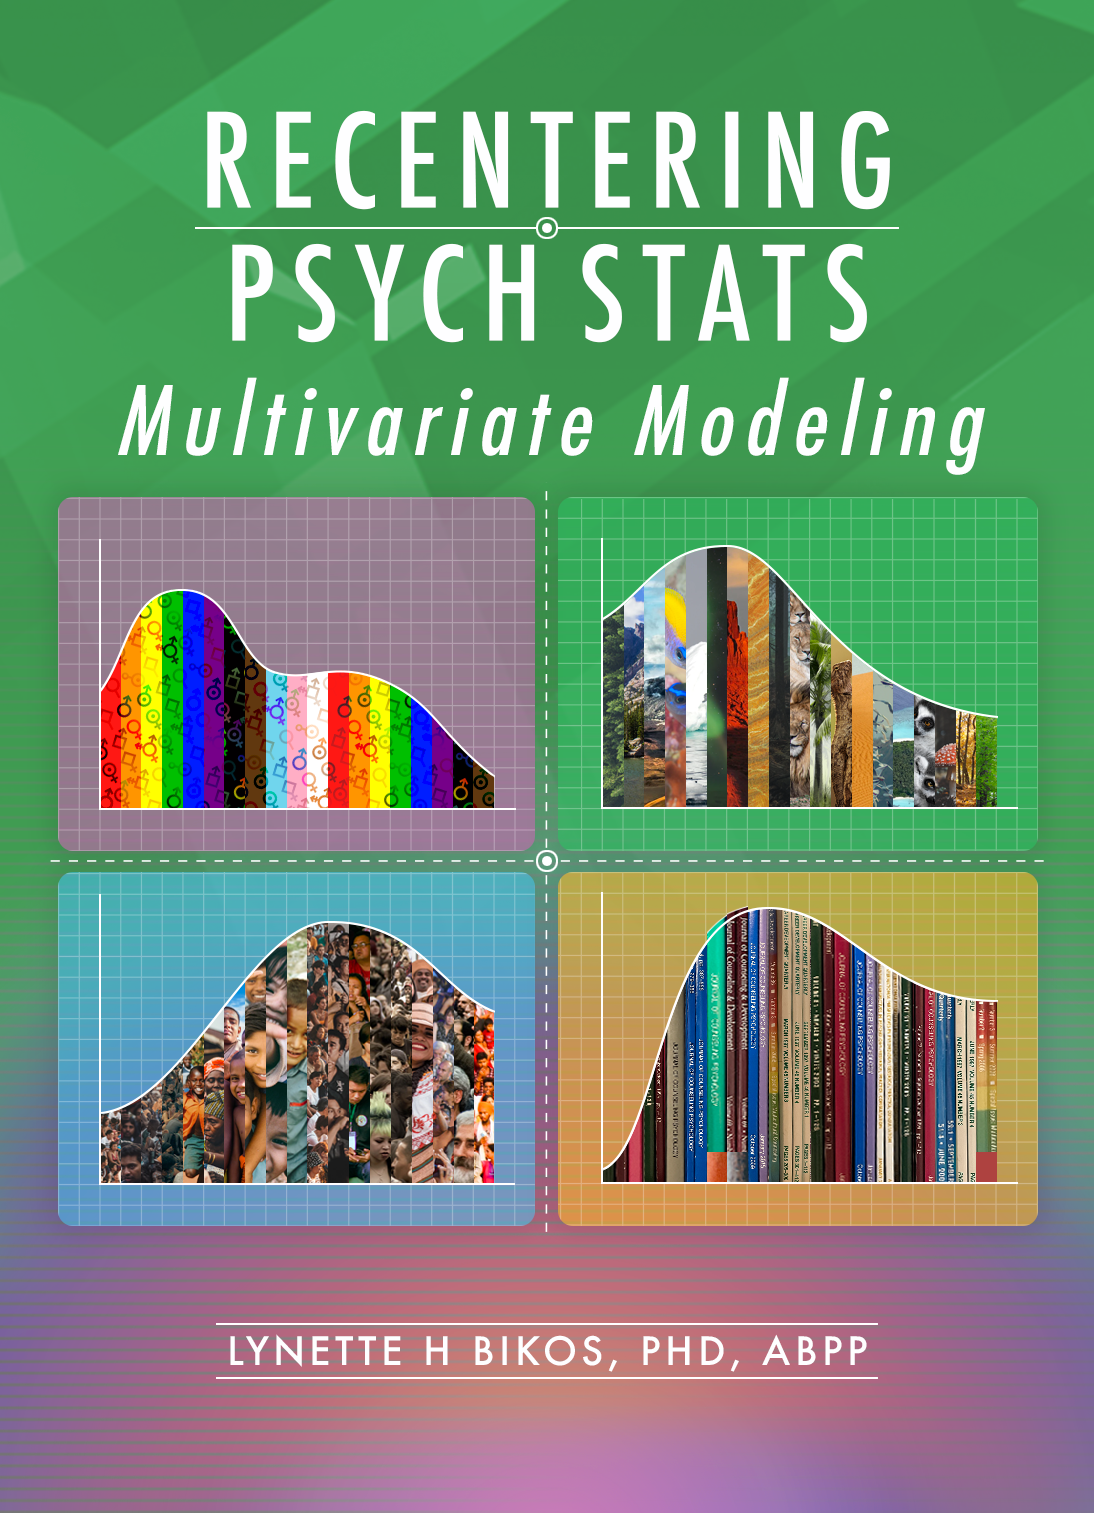
\includegraphics{images/ReC_multivariate_bkcvr.png} This open education resource is available in the following formats, all available in the \href{https://github.com/lhbikos/ReC_MultivModel/tree/main/docs}{docs} folder at the GitHub repository:

\begin{itemize}
\tightlist
\item
  Formatted as an \href{https://lhbikos.github.io/ReC_MultivModel/}{html book} via GitHub Pages available
\item
  As a \href{https://github.com/lhbikos/ReC_MultivModel/blob/main/docs/ReC_MultMod.pdf}{PDF}
\item
  As an \href{https://github.com/lhbikos/ReC_MultivModel/blob/main/docs/ReC_MultMod.epub}{ebook}
\item
  As a \href{https://github.com/lhbikos/ReC_MultivModel/blob/main/docs/ReC_MultMod.docx}{Word}
\end{itemize}

All materials used in creating this OER are available at its \href{https://github.com/lhbikos/ReC_MultivModel}{GitHub repo}.

\hypertarget{preface}{%
\chapter*{PREFACE}\label{preface}}


\textbf{If you are viewing this document, you should know that this is a book-in-progress. Early drafts are released for the purpose teaching my classes and gaining formative feedback from a host of stakeholders. The document was last updated on 04 Sep 2023}. Emerging volumes on other statistics are posted on the \href{https://lhbikos.github.io/BikosRVT/ReCenter.html}{ReCentering Psych Stats} page at my research team's website.

\href{https://spu.hosted.panopto.com/Panopto/Pages/Viewer.aspx?id=c932455e-ef06-444a-bdca-acf7012d759a}{Screencasted Lecture Link}

To \emph{center} a variable in regression means to set its value at zero and interpret all other values in relation to this reference point. Regarding race and gender, researchers often center male and White at zero. Further, it is typical that research vignettes in statistics textbooks are similarly seated in a White, Western (frequently U.S.), heteronormative, framework. The purpose of this project is to create a set of open educational resources (OER) appropriate for doctoral and post-doctoral training that contribute to a socially responsive pedagogy -- that is, it contributes to justice, equity, diversity, and inclusion.

Statistics training in doctoral programs are frequently taught with fee-for-use programs (e.g., SPSS/AMOS, SAS, MPlus) that may not be readily available to the post-doctoral professional. In recent years, there has been an increase and improvement in R packages (e.g., \emph{psych}, \emph{lavaan}) used for in analyses common to psychological research. Correspondingly, many graduate programs are transitioning to statistics training in R (free and open source). This is a challenge for post-doctoral psychologists who were trained with other software. This OER will offer statistics training with R and be freely available (specifically in a GitHub respository and posted through GitHub Pages) under a Creative Commons Attribution - Non Commercial - Share Alike license {[}CC BY-NC-SA 4.0{]}.

Training models for doctoral programs in HSP are commonly scholar-practitioner, scientist-practitioner, or clinical-scientist. An emerging model, the \emph{scientist-practitioner-advocacy} training model incorporates social justice advocacy so that graduates are equipped to recognize and address the sociocultural context of oppression and unjust distribution of resources and opportunities \citep{mallinckrodt_scientist-practitioner-advocate_2014}. In statistics textbooks, the use of research vignettes engages the learner around a tangible scenario for identifying independent variables, dependent variables, covariates, and potential mechanisms of change. Many students recall examples in Field's \citeyearpar{field_discovering_2012} popular statistics text: Viagra to teach one-way ANOVA, beer goggles for two-way ANOVA, and bushtucker for repeated measures. What if the research vignettes were more socially responsive?

In this OER, research vignettes will be from recently published articles where:

\begin{itemize}
\tightlist
\item
  the author's identity is from a group where scholarship is historically marginalized (e.g., BIPOC, LGBTQ+, LMIC{[}low-middle income countries{]}),
\item
  the research is responsive to issues of justice, equity, inclusion, diversity,
\item
  the lesson's statistic is used in the article, and
\item
  there is sufficient information in the article to simulate the data for the chapter example(s) and practice problem(s); or it is publicly available.
\end{itemize}

In training for multicultural competence, the saying, ``A fish doesn't know that it's wet'' is often used to convey the notion that we are often unaware of our own cultural characteristics. In recent months and years, there has been an increased awakening to the institutional and systemic racism that our systems are perpetuating. Queuing from the water metaphor, I am hopeful that a text that is recentered in the ways I have described can contribute to \emph{changing the water} in higher education and in the profession of psychology.

\hypertarget{copyright-with-open-access}{%
\section*{Copyright with Open Access}\label{copyright-with-open-access}}


This book is published under a a Creative Commons Attribution-NonCommercial-ShareAlike 4.0 International License. This means that this book can be reused, remixed, retained, revised and redistributed (including commercially) as long as appropriate credit is given to the authors. If you remix, or modify the original version of this open textbook, you must redistribute all versions of this open textbook under the same license - CC BY-SA.

A \href{https://github.com/lhbikos/ReC_MultivModel}{GitHub open-source repository} contains all of the text and source code for the book, including data and images.

\hypertarget{acknowledgements}{%
\chapter*{ACKNOWLEDGEMENTS}\label{acknowledgements}}


As a doctoral student at the University of Kansas (1992-2005), I learned that ``a foreign language'' was a graduation requirement. \emph{Please note that as one who studies the intersections of global, vocational, and sustainable psychology, I regret that I do not have language skills beyond English.} This could have been met with credit from high school my rural, mid-Missouri high school did not offer such classes. This requirement would have typically been met with courses taken during an undergraduate program -- but my non-teaching degree in the University of Missouri's School of Education was exempt from this. The requirement could have also been met with a computer language (fortran, C++) -- I did not have any of those either. There was a tiny footnote on my doctoral degree plan that indicated that a 2-credit course, ``SPSS for Windows'' would substitute for the language requirement. Given that it was taught by my one of my favorite professors, I readily signed up. As it turns out, Samuel B. Green, PhD, was using the course to draft chapters in the textbook \citep{green_using_2014} that has been so helpful for so many. Unfortunately, Drs. Green (1947 - 2018) and Salkind (2947 - 2017) are no longer with us. I have worn out numerous versions of their text. Another favorite text of mine was Dr.~Barbara Byrne's \citeyearpar{byrne_structural_2016}, ``Structural Equation Modeling with AMOS.'' I loved the way she worked through each problem and paired it with a published journal article, so that the user could see how the statistical evaluation fit within the larger project/article. I took my tea-stained text with me to a workshop she taught at APA and was proud of the signature she added to it (a little catfur might have fallen out). Dr.~Byrne created SEM texts for a number of statistical programs (e.g., LISREL, EQS, MPlus). As I was learning R, I wrote Dr.~Byrne, asking if she had an edition teaching SEM/CFA with R. She promptly wrote back, saying that she did not have the bandwidth to learn a new statistics package. We lost Dr.~Byrne in December 2020. I am so grateful to these role models for their contributions to my statistical training. I am also grateful for the doctoral students who have taken my courses and are continuing to provide input for how to improve the materials.

The inspiration for training materials that re*center statistics and research methods came from the \href{https://www.academics4blacklives.com/}{Academics for Black Survival and Wellness Initiative}. This project, co-founded by Della V. Mosley, Ph.D., and Pearis L. Bellamy, M.S., made clear the necessity and urgency for change in higher education and the profession of psychology.

At very practical levels, I am indebted to SPU's Library, and more specifically, SPU's Education, Technology, and Media Department. Assistant Dean for Instructional Design and Emerging Technologies, R. John Robertson, MSc, MCS, has offered unlimited consultation, support, and connection. Senior Instructional Designer in Graphics \& Illustrations, Dominic Wilkinson, designed the logo and bookcover. Psychology and Scholarly Communications Librarian, Kristin Hoffman, MLIS, has provided consultation on topics ranging from OERS to citations. I am alo indebted to Associate Vice President, Teaching and Learning at Kwantlen Polytechnic University, Rajiv Jhangiani, PhD. Dr.~Jhangiani's text \citeyearpar{jhangiani_research_2019} was the first OER I ever used and I was grateful for his encouraging conversation.

Financial support for this project has been provided the following:

\begin{itemize}
\tightlist
\item
  \emph{Call to Action on Equity, Inclusion, Diversity, Justice, and Social Responsivity Request for Proposals} grant from the Association of Psychology Postdoctoral and Internship Centers (2021-2022).
\item
  \emph{Diversity Seed Grant}, Office of Inclusive Excellence and Advisory Council for Diversity and Reconciliation (ACDR), Seattle Pacific University.
\item
  \emph{ETM Open Textbook \& OER Development Funding}, Office of Education, Technology, \& Media, Seattle Pacific University.
\end{itemize}

\hypertarget{dataprep}{%
\chapter*{DATA PREP}\label{dataprep}}


\hypertarget{scrub}{%
\chapter{Scrubbing}\label{scrub}}

\href{https://youtube.com/playlist?list=PLtz5cFLQl4KPwGvx4MHxA7C1StPkHnFH3\&si=VzB-HVlJTS07FuFw}{Screencasted Lecture Link}

The focus of this chapter is the process of starting with raw data and preparing it for multivariate analysis. To that end, we will address the conceptual considerations and practical steps in ``scrubbing and scoring.''

A twist in this lesson is that I am asking you to contribute to the dataset that serves as the basis for the chapter and the practice problems. In the spirit of \emph{open science}, this dataset is available to you and others for your own learning. Before continuing, please take 15-20 minutes to complete the survey titled, \href{https://spupsych.az1.qualtrics.com/jfe/form/SV_b2cClqAlLGQ6nLU}{Rate-a-Recent-Course: A ReCentering Psych Stats Exercise}. The study is approved by the Institutional Review Board at Seattle Pacific University (SPUIRB\# 202102011, no expiration). Details about the study, including an informed consent, are included at the link.

\hypertarget{navigating-this-lesson}{%
\section{Navigating this Lesson}\label{navigating-this-lesson}}

There is about 90 minutes of lecture. If you work through the materials with me it would be good to add another hour.

While the majority of R objects and data you will need are created within the R script that sources the chapter, there are a few that cannot be created from within the R framework. Additionally, sometimes links fail. All original materials are provided at the \href{https://github.com/lhbikos/ReC_MultivModel}{Github site} that hosts the book. More detailed guidelines for ways to access all these materials are provided in the OER's \protect\hyperlink{ReCintro}{introduction}

\hypertarget{learning-objectives}{%
\subsection{Learning Objectives}\label{learning-objectives}}

Learning objectives from this lecture include the following:

\begin{itemize}
\tightlist
\item
  Import data from Qualtrics into R.
\item
  Apply inclusion and exclusion criteria to a dataset.
\item
  Rename variables.
\item
  Create a smaller dataframe with variables appropriate for testing a specific statistical model.
\item
  Use critical data manipulation functions from the \emph{tidyverse} (and \emph{dplyr}) in particular such as \emph{filter()}, \emph{select()}, and \emph{mutate()} to prepare variables.
\item
  Articulate the initial steps in a workflow for scrubbing and scoring data.
\end{itemize}

\hypertarget{planning-for-practice}{%
\subsection{Planning for Practice}\label{planning-for-practice}}

The suggestions for practice will start with this chapter and continue in the next two chapters (Scoring, Data Dx). Using Parent's \citeyearpar{parent_handling_2013} AIA (available item analysis) approach to managing missing data, you will scrub-and-score a raw dataset. Options of graded complexity could incude:

\begin{itemize}
\tightlist
\item
  Repeating the steps in the chapter with the most recent data from the Rate-A-Recent-Course survey; differences will be in the number of people who have completed the survey since the chapter was written.
\item
  Use the dataset that is the source of the chapter, but score a different set of items that you choose.
\item
  Begin with raw data to which you have access.
\end{itemize}

\hypertarget{readings-resources}{%
\subsection{Readings \& Resources}\label{readings-resources}}

In preparing this chapter, I drew heavily from the following resource(s). Other resources are cited (when possible, linked) in the text with complete citations in the reference list.

\begin{itemize}
\tightlist
\item
  Parent, M. C. (2013). Handling item-level missing data: Simpler is just as good. The Counseling Psychologist, 41(4), 568--600. \url{https://doi.org/10.1177/0011000012445176}

  \begin{itemize}
  \tightlist
  \item
    The purpose of Parent's article was to argue that complex and resource-intensive procedurs like multiple imputation are unnecessary. Following a simulation that supports his claims, Parent provides some guidelines to follow for the AIA approach.
  \end{itemize}
\item
  Kline, R. B. (2015). Data preparation and psychometrics review. In Principles and Practice of Structural Equation Modeling, Fourth Edition. Guilford Publications. \url{http://ebookcentral.proquest.com/lib/spu/detail.action?docID=4000663}

  \begin{itemize}
  \tightlist
  \item
    Kline's chapter is my ``go-to'' for making decisions about preparing data for analysis.
  \end{itemize}
\end{itemize}

\hypertarget{packages}{%
\subsection{Packages}\label{packages}}

The script below will (a) check to see if the following packages are installed on your computer and, if not (b) install them.

\begin{Shaded}
\begin{Highlighting}[]
\CommentTok{\# will install the package if not already installed}
\CommentTok{\# if(!require(qualtRics))\{install.packages(\textquotesingle{}qualtRics\textquotesingle{})\}}
\CommentTok{\# if(!require(tidyverse))\{install.packages(\textquotesingle{}tidyverse\textquotesingle{})\}}
\end{Highlighting}
\end{Shaded}

\hypertarget{workflow-for-scrubbing}{%
\section{Workflow for Scrubbing}\label{workflow-for-scrubbing}}

The same workflow guides us through the Scrubbing, Scoring, and Data Dx chapters. In this lesson we focus on downloading data from Qualtrics and determining which cases can be retained for analysis based on inclusion and exclusion criteria.

\begin{figure}
\centering
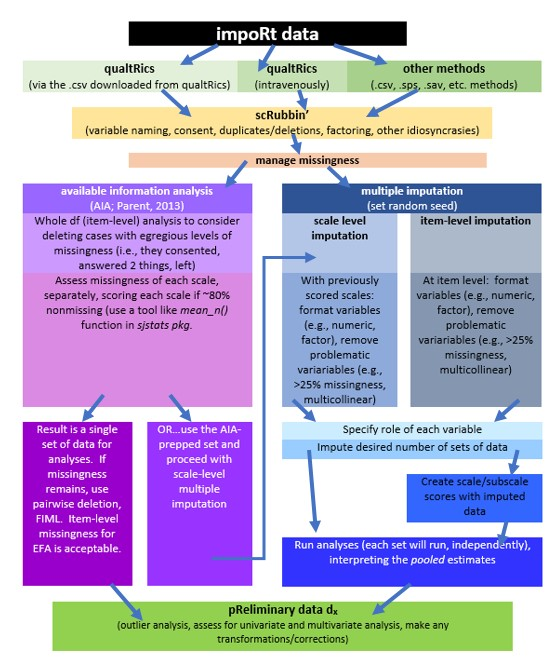
\includegraphics{images/Ch02/scrubscore_wrkflow.jpg}
\caption{An image of a workflow for scrubbing and scoring data.}
\end{figure}

Here is a narration of the figure:

\begin{enumerate}
\def\labelenumi{\arabic{enumi}.}
\tightlist
\item
  The workflow begins by importing data into R. Most lessons in this series involve simulated data that are created directly in R. Alternatively, data could be:

  \begin{itemize}
  \tightlist
  \item
    imported ``intRavenously'' through programs such as Qualtrics,
  \item
    exported from programs such as Qualtrics to another program (e.g., .xlxs, .csv),
  \item
    imported in other forms (e.g., .csv, .sps, .sav).
  \end{itemize}
\item
  Scrubbing data by

  \begin{itemize}
  \tightlist
  \item
    variable naming,
  \item
    specifying variable characteristics such as factoring,
  \item
    ensuring that included participants consented to participation,
  \item
    determining and executing the inclusion and exclusion criteria.
  \end{itemize}
\item
  Conduct preliminary data diagnostics such as

  \begin{itemize}
  \tightlist
  \item
    outlier analysis
  \item
    assessing for univariate and multivariate analysis
  \item
    making transformations and/or corrections
  \end{itemize}
\item
  Managing missingness by one of two routes

  \begin{itemize}
  \tightlist
  \item
    Available information analysis \citep{parent_handling_2013} at either the item-level or scale level. The result is a single set of data for analysis. If missingness remains, options include pairwise deletion, listwise deletion, or specifying FIML (when available). Another option is to use multiple imputation.
  \item
    Multiple imputation at either scale level or item-level
  \end{itemize}
\end{enumerate}

\hypertarget{research-vignette}{%
\section{Research Vignette}\label{research-vignette}}

To provide first-hand experience as both the respondent and analyst for the same set of data, you were asked to complete a survey titled, \href{https://spupsych.az1.qualtrics.com/jfe/form/SV_b2cClqAlLGQ6nLU}{Rate-a-Recent-Course: A ReCentering Psych Stats Exercise}. If you haven't yet completed it, please consider doing so, now. In order to reduce the potential threats to validity by providing background information about the survey, I will wait to describe it until later in the chapter.

The survey is administered in Qualtrics. In the chapter I teach two ways to import Qualtrics data into R. We will then use the data to work through the steps identified in the workflow.

\hypertarget{working-the-problem}{%
\section{Working the Problem}\label{working-the-problem}}

\hypertarget{intravenous-qualtrics}{%
\subsection{intRavenous Qualtrics}\label{intravenous-qualtrics}}

I will demonstrate using a Qualtrics account at my institution, Seattle Pacific University. The only surveys in this account are for the \emph{Recentering Psych Stats} chapters and lessons. The surveys were designed to not capture personally identifying information.

Access credentials for the institutional account, individual user's account, and survey are essential for getting the survey items and/or results to export into R. The Qualtrics website provides a tutorial for \href{https://www.qualtrics.com/support/integrations/api-integration/overview/\#GeneratingAnAPIToken}{generating an API token}.

We need two pieces of information: the \textbf{root\_url} and an \textbf{API token}. To retrieve these:

\begin{itemize}
\tightlist
\item
  Log into your respective qualtrics.com account
\item
  Select Account Settings
\item
  Choose ``Qualtrics IDs'' from the user name dropdown
\end{itemize}

The \textbf{root\_url} is the first part of the web address for the Qualtrics account. For our institution it is: \emph{spupsych.az1.qualtrics.com }.

The API token is in the box labeled, ``API.'' If it is empty, select, ``Generate Token.'' If you do not have this option, locate the \emph{brand administrator} for your Qualtrics account. They will need to set up your account so that you have API privileges.

\emph{BE CAREFUL WITH THE API TOKEN} This is the key to your Qualtrics accounts. If you leave it in an .rmd file that you forward to someone else or upload to a data repository, this key and the base URL gives access to every survey in your account. If you share it, you could be releasing survey data to others that would violate confidentiality promises in an IRB application.

If you mistakenly give out your API token you can generate a new one within your Qualtrics account and re-protect all its contents.

You do need to change the API key/token if you want to download data from a different Qualtrics account. If your list of surveys generates the wrong set of surveys, restart R, make sure you have the correct API token and try again.

\begin{Shaded}
\begin{Highlighting}[]
\CommentTok{\# You only need to run this ONCE to draw from the same Qualtrics}
\CommentTok{\# account. If you change Qualtrics accounts you will need to get a}
\CommentTok{\# different token.}

\CommentTok{\# qualtRics::qualtrics\_api\_credentials(api\_key =}
\CommentTok{\# \textquotesingle{}mUgPMySYkiWpMFkwHale1QE5HNmh5LRUaA8d9PDg\textquotesingle{}, base\_url =}
\CommentTok{\# \textquotesingle{}spupsych.az1.qualtrics.com\textquotesingle{}, overwrite = TRUE, install = TRUE)}

\CommentTok{\# readRenviron(\textquotesingle{}\textasciitilde{}/.Renviron\textquotesingle{})}
\end{Highlighting}
\end{Shaded}

\emph{all\_surveys()} generates a dataframe containing information about all the surveys stored on your Qualtrics account.

\begin{Shaded}
\begin{Highlighting}[]
\CommentTok{\# surveys \textless{}{-} qualtRics::all\_surveys()}

\CommentTok{\# View this as an object (found in the right: Environment).  Get}
\CommentTok{\# survey id \# for the next command If this is showing you the WRONG}
\CommentTok{\# list of surveys, you are pulling from the wrong Qualtrics account}
\CommentTok{\# (i.e., maybe this one instead of your own). Go back and change your}
\CommentTok{\# API token (it saves your old one). Changing the API likely requires}
\CommentTok{\# a restart of R.}
\end{Highlighting}
\end{Shaded}

To retrieve the survey, use the \emph{fetch\_survey()} function.

\begin{Shaded}
\begin{Highlighting}[]
\CommentTok{\# obtained with the survey ID}
\CommentTok{\#\textquotesingle{}surveyID\textquotesingle{} should be the ID from above}
\CommentTok{\#\textquotesingle{}verbose\textquotesingle{} prints messages to the R console}
\CommentTok{\#\textquotesingle{}label\textquotesingle{}, when TRUE, imports data as text responses; if FALSE prints the data as numerical responses}
\CommentTok{\#\textquotesingle{}convert\textquotesingle{}, when TRUE, attempts to convert certain question types to the \textquotesingle{}proper\textquotesingle{} data type in R; because I don\textquotesingle{}t like guessing, I want to set up my own factors.}
\CommentTok{\#\textquotesingle{}force\_request\textquotesingle{}, when TRUE, always downloads the survey from the API instead of from a temporary directory (i.e., it always goes to the primary source)}
\CommentTok{\# \textquotesingle{}import\_id\textquotesingle{}, when TRUE includes the unique Qualtrics{-}assigned ID;}
\CommentTok{\# since I have provided labels, I want false}

\NormalTok{QTRX\_df }\OtherTok{\textless{}{-}}\NormalTok{ qualtRics}\SpecialCharTok{::}\FunctionTok{fetch\_survey}\NormalTok{(}\AttributeTok{surveyID =} \StringTok{"SV\_b2cClqAlLGQ6nLU"}\NormalTok{, }\AttributeTok{time\_zone =} \ConstantTok{NULL}\NormalTok{,}
    \AttributeTok{verbose =} \ConstantTok{FALSE}\NormalTok{, }\AttributeTok{label =} \ConstantTok{FALSE}\NormalTok{, }\AttributeTok{convert =} \ConstantTok{FALSE}\NormalTok{, }\AttributeTok{force\_request =} \ConstantTok{TRUE}\NormalTok{,}
    \AttributeTok{import\_id =} \ConstantTok{FALSE}\NormalTok{)}

\CommentTok{\# useLocalTime = TRUE,}
\end{Highlighting}
\end{Shaded}

\emph{It is possible to import Qualtrics data that has been downloaded from Qualtrics as a .csv. I demo this in the Bonus Reel at the end of this lesson.}

In prior versions of this chapter I allowed the chapter to automatically update with ``all the new data'' each time the OER was re-rendered/built. Because I think this caused confusion, I have decided to save the data in both .csv and .rds versions, then clear my environment, upload the .rds (my personal favorite format) version, and demonstrate the scrubbing techniques with that data. If you continue with data you just downloaded from Qualtrics, you will get different answers than are in the lesson. While I think that continuing with the most current data set is a viable option for a practice problem, it could be confusing. Rather, follow one of the two options below to upload .csv or .rds versions of the data I used in the lesson.

\hypertarget{option-1.-upload-an-.rds-file}{%
\subsubsection{Option 1. Upload an .rds file}\label{option-1.-upload-an-.rds-file}}

Because .rds files will retain any formatting information we provide about variables, I like using them. The downside is that you cannot simply open and view them outside of the R environment. Here is the code I used to produce the .rds version of the file. If you want to obtain the same results as I report in the chapter, do NOT run it again.

\begin{Shaded}
\begin{Highlighting}[]
\CommentTok{\# to save the df as an .rds (think \textquotesingle{}R object\textquotesingle{}) file on your computer;}
\CommentTok{\# it should save in the same file as the .rmd file you are working}
\CommentTok{\# with saveRDS(QTRX\_df, \textquotesingle{}QTRX\_df230902.rds\textquotesingle{})}
\end{Highlighting}
\end{Shaded}

Rather, head to the \href{https://github.com/lhbikos/ReC_MultivModel}{MultivModel GitHub} site and download the \emph{QTRX\_df230902b.rds} file. Place it in the same folder as the .rmd you are using and run the code below. And actually, I further re-named the file that you will retrieve so that it won't be over-written.*

\begin{Shaded}
\begin{Highlighting}[]
\NormalTok{QTRX\_df }\OtherTok{\textless{}{-}} \FunctionTok{readRDS}\NormalTok{(}\StringTok{"QTRX\_df230902b.rds"}\NormalTok{)}
\end{Highlighting}
\end{Shaded}

Occasionally, I have had a student for whom the .rds files don't seem to work. Uploading a .csv file is an option.

\hypertarget{option-2.-upload-a-.csv-file}{%
\subsubsection{Option 2. Upload a .csv file}\label{option-2.-upload-a-.csv-file}}

Simply for your information, here is the code I used to produce the .csv version of the file. If you want to obtain the same results as I report in the chapter, do NOT run it again.

\begin{Shaded}
\begin{Highlighting}[]
\CommentTok{\# write the simulated data as a .csv write.table(QTRX\_df,}
\CommentTok{\# file=\textquotesingle{}QTRX\_df230902.csv\textquotesingle{}, sep=\textquotesingle{},\textquotesingle{}, col.names=TRUE, row.names=FALSE)}
\end{Highlighting}
\end{Shaded}

Rather, head to the \href{https://github.com/lhbikos/ReC_MultivModel}{MultivModel GitHub} site and download the \emph{QTRX\_df230902b.csv} file. Place it in the same folder as the .rmd you are using and run the code below. \emph{And actually, I further re-named the file that you will retrieve so that it won't be over-written.}

\begin{Shaded}
\begin{Highlighting}[]
\CommentTok{\# bring back the simulated dat from a .csv file QTRX\_df \textless{}{-}}
\CommentTok{\# read.csv(\textquotesingle{}QTRX\_df230902b.csv\textquotesingle{}, header = TRUE)}
\end{Highlighting}
\end{Shaded}

You need not do both. That is, either download-and-import either the .rds or .csv file.

\hypertarget{about-the-rate-a-recent-course-survey}{%
\subsection{\texorpdfstring{About the \emph{Rate-a-Recent-Course} Survey}{About the Rate-a-Recent-Course Survey}}\label{about-the-rate-a-recent-course-survey}}

As a teaching activity for the ReCentering Psych Stats OER, the topic of the survey was selected to be consistent with the overall theme of OER. Specifically, the purpose of this study is to understand the campus climate for students whose identities make them vulnerable to bias and discrimination. These include students who are Black, non-Black students of color, LGBTQ+ students, international students, and students with disabilities.

Although the dataset should provide the opportunity to test a number of statistical models, one working hypothesis that framed the study is that the there will be a greater sense of belonging and less bias and discrimination when there is similar representation (of identities that are often marginalized) in the instructional faculty and student body. Termed, ``structural diversity'' \citep{lewis_black_2019} this is likely an oversimplification. In fact, an increase in diverse representation without attention to interacting factors can increase hostility on campus \citep{hurtado_linking_2007}. Thus, we included the task of rating of a single course relates to the larger campus along the dimensions of belonging and bias/discrimination. For example, if a single class has higher ratings on issues of inclusivity, diversity, and respect, we would expect that sentiment to be echoed in the broader institution.

Our design has notable limitations You will likely notice that we ask about demographic characteristics of the instructional staff and classmates in the course rated, but we do not ask about the demographic characteristics of the respondent. In making this decision, we likely lose important information; Iacovino and James \citeyearpar{iacovino_retaining_2016} have noted that White students perceive campus more favorably than Black student counterparts. We made this decision to protect the identity of the respondent. As you will see when we download the data, if a faculty member asked an entire class to take the survey, the datestamp and a handful of demographic identifiers could very likely identify a student. In certain circumstances, this might be risky in that private information (i.e., gender nonconformity, disclosure of a disability) or course evaluation data could be related back to the student.

Further, the items that ask respondents to \emph{guess} the identities of the instructional staff and classmates are limited, and contrary to best practices in survey construction that recommend providing the option of a ``write-in'' a response. After consulting with a diverse group of stakeholders and subject matter experts (and revising the response options numerous times) I have attempted to center anti-Black racism in the U.S. \citep{mosley_critical_2021, mosley_radical_2020, singh_building_2020}. In fact, the display logic does not present the race items when the course is offered outside the U.S. There are only five options for race: \emph{biracial/multiracial}, \emph{Black}, \emph{non-Black person(s) of color}, \emph{White}, and \emph{I did not notice} (intended to capture a color-blind response). One unintended negative consequence of this design is that the response options could contribute to \emph{colorism} \citep{adames_fallacy_2021, capielo_rosario_acculturation_2019}. Another possibility is that the limited options may erase, or make invisible, other identities. At the time that I am writing the first draft of this chapter, the murder of six Asian American women in Atlanta has just occurred. The Center for the Study of Hate and Extremeism has documented that while overall hate crimes dropped by 7\% in 2020, anti-Asian hate crimes reported to the police in America's largest cities increasedby 149\% \citep{noauthor_fact_nodate}. These incidents have occurred not only in cities, but in our neighborhoods and on our campusus \citep{kim_guest_2021, kim_yes_2021, noauthor_stop_nodate}. While this survey is intended to assess campus climate as a function of race, it unfortunately does not distinguish between many identities that experience marginalization.

In parallel, the items asking respondents to identity characteristics of the instructional staff along dimensions of gender, international status, and disability are ``large buckets'' and do not include ``write-in'' options. Similarly, there was no intent to cause harm by erasing or making invisible individuals whose identities are better defined by different descriptors. Further, no write-in items were allowed. This was also intentional to prevent potential harm caused by people who could leave inappropriate or harmful comments.

\hypertarget{the-codebook}{%
\subsection{The Codebook}\label{the-codebook}}

In order to scrub-and-score a survey, it is critical to know about its content, scoring directions for scales/subscales, and its design. A more complete description of the survey design elements is (or will be) available in the \emph{Recentering Psych Stats: Psychometric} OER. The review in this chapter provides just-enough information to allow us to make decisions about which items to retain and how to score them. When they are well-written, information in the \href{./Bikos_ReCenteringPsychStats_ReCupload.pdf}{IRB application} and \href{https://osf.io/a8e5u}{pre-registration} can be helpful in the scrubbing and scoring process.

Let's look ``live'' at the survey. In Qualtrics it is possible to \emph{print} a PDF that looks very similar to its presentation when someone is taking it. You can access that static version \href{./Rate_a_CoursePDF.pdf}{here}.

We can export a \href{./Rate-a-Course_Codebook.pdf}{codebook}, that is, a Word (or PDF) version of the survey with all the coding. In Qualtrics the protocol is: Survey/Tools/ImportExport/Export Survey to Word. Then select all the options you want (especially ``Show Coded Values''). A tutorial provided by Qualtrics can be found \href{https://www.qualtrics.com/support/survey-platform/survey-module/survey-tools/import-and-export-surveys/}{here}. This same process can be used to print the PDF example I used above.

It is almost impossible to give this lecture without some reference to Qualtrics and the features used in Qualtrics. An import of raw data from Qualtrics into R can be nightmare in that the Qualtrics-assigned variable names are numbers (e.g., QID1, QID2) -- but often out of order because the number is assigned when the question is first created. If the survey is reordered, the numbers get out of sequence.

Similarly, values for Likert-type scales can also get out of order if the scale anchors are revised (which is common to do).

I recommend providing custom variable names and recode values directly in Qualtrics before exporting them into R. A Qualtrics tutorial for this is provided \href{https://www.qualtrics.com/support/survey-platform/survey-module/question-options/recode-values/}{here}. In general, consider these qualities when creating variable names:

\begin{itemize}
\tightlist
\item
  Brevity: historically, SPSS variable names could be a maximum of 8 characters.
\item
  Intuitive: although variables can be renamed in R (e.g., for use in charts and tables), it is helpful when the name imported from Qualtrics provides some indication of what the variable is.
\item
  Systematic: start items in a scale with the same stem, followed by the item number -- ITEM1, ITEM2, ITEM3.
\end{itemize}

The Rate-a-Recent-Course survey was written using some special features in Qualtrics. These include

\begin{itemize}
\tightlist
\item
  Display logic

  \begin{itemize}
  \tightlist
  \item
    Items that are U.S.-centric are only shown if the respondent is taking a course from an institution in the U.S. is a student in the U.S.
  \end{itemize}
\item
  Loop and merge

  \begin{itemize}
  \tightlist
  \item
    Because course may have multiple instructional staff, the information asking about demographic characteristics of the instructors is repeated according to the number input by the respondent
  \end{itemize}
\item
  Random presentation of the 30 items asking about campus climate for the five groups of students

  \begin{itemize}
  \tightlist
  \item
    Although this might increase the cognitive load of the survey, this helps ``spread out'' missingness for respondents who might tire of the survey and stop early
  \end{itemize}
\item
  Rank ordering of the institutional level (department, school/faculty, campus/university) to which the respondent feels most connected
\end{itemize}

Looking at the QTRX\_df, \emph{StartDate} thru \emph{UserLanguage} are metadata created by Qualtrics. The remaining variables and associated value labels are in the \href{./Rate-a-Course_Codebook.pdf}{codebook}.

\hypertarget{scrubbing}{%
\section{Scrubbing}\label{scrubbing}}

With a look at our survey, codebook, and imported data, we now get to the business of scRubbing (deleting those who did not give consent, deleting previews, etc.). This level of ``scrubbing'' precedes the more formal detection of outliers.

\hypertarget{tools-for-data-manipulation}{%
\subsection{Tools for Data Manipulation}\label{tools-for-data-manipulation}}

The next stages will provide some experience manipulating data with \textbf{dplyr} from the \textbf{tidyverse}.

The \textbf{tidyverse} is a system of packages (i.e,. when you download the tidyverse, you download all its packages/members) for data manipulation, exploration and visualization. The packages in the tidyverse share a common design philosophy. These were mostly developed by Hadley Wickham, but more recently, more designers are contributing to them. Tidyverse packages are intended to make statisticians and data scientists more productive by guiding them through workflows that facilitate communication and result in reproducible work products. Fundamentally, the tidyverse is about the connections between the tools that make the workflow possible. Critical packages in the tidyverse include:

\begin{itemize}
\tightlist
\item
  \textbf{dplyr}: data manipulation: mutate, select, filter, summarize, arrange
\item
  \textbf{ggplot2}: extravagant graphing
\item
  \textbf{tibble}: a \emph{tibble} is a dataframe that provides the user with more (and less) control over the data.
\item
  \textbf{readr}: gives access to ``rectangular data'' like .csv and tables
\item
  \textbf{tidyr}: tidy data is where each variable is a column, each observation is a row, each value is a cell (duh). \textbf{tidyr}'s contributions are gather(wide to long) and spread(long to wide) as well as separate, extract, unite.
\item
  \textbf{purrr}: facilitates working with functions and vectors. For example, if you write a function, using purrr may help you replace loops with code that is more efficient and intuitive.
\end{itemize}

The tidyverse is ever-evolving -- so check frequently for updates and troubleshooting.

A handy cheatsheet for data transformation is found \href{https://www.rstudio.com/wp-content/uploads/2015/02/data-wrangling-cheatsheet.pdf}{here}.

\hypertarget{inclusion-and-exclusion-criteria}{%
\subsection{Inclusion and Exclusion Criteria}\label{inclusion-and-exclusion-criteria}}

For me, the first pass at scrubbing is to eliminate the obvious. In our case this is includes \emph{previews} and respondents who did not consent to continue. Previews are the researcher-initiated responses usually designed to proofread or troubleshoot survey problems. There could be other first-pass-deletions, such as selecting response between certain dates.

I think these first-pass deletions, especially the ones around consent, are important to do as soon as possible. Otherwise, we might delete some of the variables (e.g., timestamps, consent documentation, preview status) and neglect to delete these cases later in the process.

We are here in the workflow:

\begin{figure}
\centering
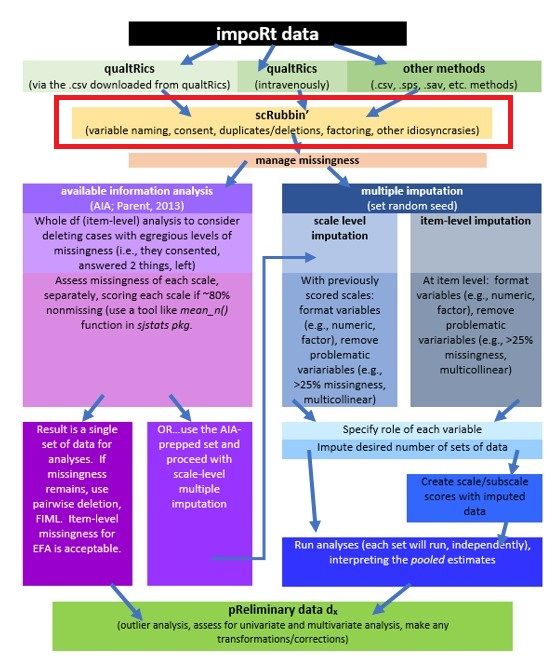
\includegraphics{images/Ch02/wrkflow_prelim.jpg}
\caption{An image of a workflow for scrubbing and scoring data.}
\end{figure}

We can either update the existing df (by using the same object), or creating a new df from the old. Either works. In my early years, I tended to create lots of new objects. As I have gained confidence in myself and in R, I'm inclined to update the existing df. Why? Because unless you write the object as an outfile (using the same name for the object as for the filename -- which I do not recommend), the object used in R does not change the source of the dat. Therefore, it is easy to correct early code and it keeps the global environment less cluttered.

In this particular survey, the majority of respondents will take the survey because they clicked an \emph{anonymous} link provided by Qualtrics. Another Qualtrics distribution method is e-mail. At the time of this writing, we have not recruited by e-mail, but it is is possible we could do so in the future. What we should not include, though, are \emph{previews}. These are the times when the researcher is self-piloting the survey to look for errors and to troubleshoot.

\begin{Shaded}
\begin{Highlighting}[]
\CommentTok{\# the filter command is used when we are making inclusion/exclusion}
\CommentTok{\# decisions about rows != means do not include cases with \textquotesingle{}preview\textquotesingle{}}

\NormalTok{QTRX\_df }\OtherTok{\textless{}{-}}\NormalTok{ dplyr}\SpecialCharTok{::}\FunctionTok{filter}\NormalTok{(QTRX\_df, DistributionChannel }\SpecialCharTok{!=} \StringTok{"preview"}\NormalTok{)}

\CommentTok{\# FYI, another way that doesn\textquotesingle{}t use tidyverse, but gets the same}
\CommentTok{\# result QTRX\_df \textless{}{-} QTRX\_df[!QTRX\_df$DistributionChannel ==}
\CommentTok{\# \textquotesingle{}preview\textquotesingle{},]}
\end{Highlighting}
\end{Shaded}

APA Style, and in particular the Journal Article Reporting Standards (JARS) for quantitative research specify that we should report the frequency or percentages of missing data. We would start our counting \emph{after} eliminating the previews.

\begin{Shaded}
\begin{Highlighting}[]
\CommentTok{\# I created an object that lists how many rows/cases remain.  I used}
\CommentTok{\# inline text below to update the text with the new number}
\FunctionTok{nrow}\NormalTok{(QTRX\_df)}
\end{Highlighting}
\end{Shaded}

\begin{verbatim}
[1] 107
\end{verbatim}

CAPTURING RESULTS FOR WRITING IT UP:

\begin{quote}
\begin{quote}
Data screening suggested that 107 individuals opened the survey link.
\end{quote}
\end{quote}

Next let's filter in only those who consented to take the survey. Because Qualtrics discontinued the survey for everyone who did not consent, we do not have to worry that their data is unintentionally included, but it can be useful to mention the number of non-consenters in the summary of missing data.

\begin{Shaded}
\begin{Highlighting}[]
\CommentTok{\# == are used}
\NormalTok{QTRX\_df }\OtherTok{\textless{}{-}}\NormalTok{ dplyr}\SpecialCharTok{::}\FunctionTok{filter}\NormalTok{(QTRX\_df, Consent }\SpecialCharTok{==} \DecValTok{1}\NormalTok{)}
\FunctionTok{nrow}\NormalTok{(QTRX\_df)}
\end{Highlighting}
\end{Shaded}

\begin{verbatim}
[1] 83
\end{verbatim}

CAPTURING RESULTS FOR WRITING IT UP:

\begin{quote}
\begin{quote}
Data screening suggested that 107 individuals opened the survey link. Of those, 83 granted consent and proceeded into the survey items.
\end{quote}
\end{quote}

In this particular study, the categories used to collect informtaion about race/ethnicity were U.S.-centric. Thus, they were only shown if the respondent indicated that the course being rated was taught by an institution in the U.S. Therefore, an an additional inclusion criteria for this specific research model should be that the course was taught in the U.S.

\begin{Shaded}
\begin{Highlighting}[]
\NormalTok{QTRX\_df }\OtherTok{\textless{}{-}}\NormalTok{dplyr}\SpecialCharTok{::}\FunctionTok{filter}\NormalTok{(QTRX\_df, USinst }\SpecialCharTok{==} \DecValTok{0}\NormalTok{)}
\FunctionTok{nrow}\NormalTok{(QTRX\_df)}
\end{Highlighting}
\end{Shaded}

\begin{verbatim}
[1] 69
\end{verbatim}

CAPTURING RESULTS FOR WRITING IT UP:

\begin{quote}
\begin{quote}
Data screening suggested that 107 individuals opened the survey link. Of those, 83 granted consent and proceeded into the survey items. A further inclusion criteria was that the course was taught in the U.S; 69 met this criteria.
\end{quote}
\end{quote}

\hypertarget{renaming-variables}{%
\subsection{Renaming Variables}\label{renaming-variables}}

Even though we renamed the variables in Qualtrics, the loop-and-merge variables were auto-renamed such that they each started with a number. I cannot see how to rename these from inside Qualtrics. A potential problem is that, in R, when variable names start with numbers, they need to be surrounded with single quotation marks. I find it easier to rename them now. I used ``i'' to start the variable name to represent ``instructor.''

The form of the \emph{rename()} function is this: df\_named \textless- rename(df\_raw, NewName1 = OldName1)

\begin{Shaded}
\begin{Highlighting}[]
\NormalTok{QTRX\_df }\OtherTok{\textless{}{-}}\NormalTok{ dplyr}\SpecialCharTok{::}\FunctionTok{rename}\NormalTok{(QTRX\_df, }\AttributeTok{iRace1 =} \StringTok{"1\_iRace"}\NormalTok{, }\AttributeTok{iRace2 =} \StringTok{"2\_iRace"}\NormalTok{,}
    \AttributeTok{iRace3 =} \StringTok{"3\_iRace"}\NormalTok{, }\AttributeTok{iRace4 =} \StringTok{"4\_iRace"}\NormalTok{, }\AttributeTok{iRace5 =} \StringTok{"5\_iRace"}\NormalTok{, }\AttributeTok{iRace6 =} \StringTok{"6\_iRace"}\NormalTok{,}
    \AttributeTok{iRace7 =} \StringTok{"7\_iRace"}\NormalTok{, }\AttributeTok{iRace8 =} \StringTok{"8\_iRace"}\NormalTok{, }\AttributeTok{iRace9 =} \StringTok{"9\_iRace"}\NormalTok{, }\AttributeTok{iRace10 =} \StringTok{"10\_iRace"}\NormalTok{)}
\end{Highlighting}
\end{Shaded}

Also in Qualtrics, it was not possible to rename the variable (formatted with sliders) that asked respondents to estimate the proportion of classmates in each race-based category. Using the codebook, we can do this now. I will use ``cm'' to precede each variable name to represent ``classmates.''

\begin{Shaded}
\begin{Highlighting}[]
\NormalTok{QTRX\_df }\OtherTok{\textless{}{-}}\NormalTok{ dplyr}\SpecialCharTok{::}\FunctionTok{rename}\NormalTok{(QTRX\_df, }\AttributeTok{cmBiMulti =}\NormalTok{ Race\_10, }\AttributeTok{cmBlack =}\NormalTok{ Race\_1,}
    \AttributeTok{cmNBPoC =}\NormalTok{ Race\_7, }\AttributeTok{cmWhite =}\NormalTok{ Race\_8, }\AttributeTok{cmUnsure =}\NormalTok{ Race\_2)}
\end{Highlighting}
\end{Shaded}

Let's also create an ID variable (different from the lengthy Qualtrics-issued ID) and then move it to the front of the distribution.

\begin{Shaded}
\begin{Highlighting}[]
\CommentTok{\# Opening the tidyverse so that I can use pipes}
\FunctionTok{library}\NormalTok{(tidyverse)}
\end{Highlighting}
\end{Shaded}

\begin{verbatim}
-- Attaching core tidyverse packages ------------------------ tidyverse 2.0.0 --
v dplyr     1.1.2     v readr     2.1.4
v forcats   1.0.0     v stringr   1.5.0
v ggplot2   3.4.3     v tibble    3.2.1
v lubridate 1.9.2     v tidyr     1.3.0
v purrr     1.0.1     
-- Conflicts ------------------------------------------ tidyverse_conflicts() --
x dplyr::filter() masks stats::filter()
x dplyr::lag()    masks stats::lag()
i Use the conflicted package (<http://conflicted.r-lib.org/>) to force all conflicts to become errors
\end{verbatim}

\begin{Shaded}
\begin{Highlighting}[]
\NormalTok{QTRX\_df }\OtherTok{\textless{}{-}}\NormalTok{ QTRX\_df }\SpecialCharTok{\%\textgreater{}\%}
\NormalTok{    dplyr}\SpecialCharTok{::}\FunctionTok{mutate}\NormalTok{(}\AttributeTok{ID =} \FunctionTok{row\_number}\NormalTok{())}

\CommentTok{\# moving the ID number to the first column; requires}
\NormalTok{QTRX\_df }\OtherTok{\textless{}{-}}\NormalTok{ QTRX\_df }\SpecialCharTok{\%\textgreater{}\%}
\NormalTok{    dplyr}\SpecialCharTok{::}\FunctionTok{select}\NormalTok{(ID, }\FunctionTok{everything}\NormalTok{())}
\end{Highlighting}
\end{Shaded}

\hypertarget{downsizing-the-dataframe}{%
\subsection{Downsizing the Dataframe}\label{downsizing-the-dataframe}}

Although researchers may differ in their approach, my tendency is to downsize the df to the variables I will be using in my study. These could include variables in the model, demographic variables, and potentially auxiliary variables (i.e,. variables not in the model, but that might be used in the case of multiple imputation).

This particular survey did not collect demographic information, so that will not be used. The model that I will demonstrate in this research vignette examines the the respondent's perceived campus climate for students who are Black, predicted by the the respondent's own campus belonging, and also the \emph{structural diversity} \citep{lewis_black_2019} proportions of Black students in the classroom and BIPOC (Black, Indigenous, and people of color) instructional staff.

\emph{I would like to assess the model by having the instructional staff variable to be the \%Black instructional staff. At the time that this lecture is being prepared, there is not sufficient Black representation in the staff to model this.}

The \emph{select()} function can let us list the variables we want to retain.

\begin{Shaded}
\begin{Highlighting}[]
\CommentTok{\# You can use the \textquotesingle{}:\textquotesingle{} to include all variables from the first to last}
\CommentTok{\# variable in any sequence; I could have written this more}
\CommentTok{\# efficiently.  I just like to \textquotesingle{}see\textquotesingle{} my scales and clusters of}
\CommentTok{\# variables.}

\NormalTok{Model\_df }\OtherTok{\textless{}{-}}\NormalTok{ (dplyr}\SpecialCharTok{::}\FunctionTok{select}\NormalTok{(QTRX\_df, ID, iRace1, iRace2, iRace3, iRace4,}
\NormalTok{    iRace5, iRace6, iRace7, iRace8, iRace9, iRace10, cmBiMulti, cmBlack,}
\NormalTok{    cmNBPoC, cmWhite, cmUnsure, Belong\_1}\SpecialCharTok{:}\NormalTok{Belong\_3, Blst\_1}\SpecialCharTok{:}\NormalTok{Blst\_6))}
\end{Highlighting}
\end{Shaded}

It can be helpful to save outfile of progress as we go along. Here I save this raw file. I will demonstrate how to save both .rds and .csv files.

\begin{Shaded}
\begin{Highlighting}[]
\CommentTok{\# to save the df as an .rds (think \textquotesingle{}R object\textquotesingle{}) file on your computer;}
\CommentTok{\# it should save in the same file as the .rmd file you are working}
\CommentTok{\# with saveRDS(Model\_df, \textquotesingle{}BlackStntsModel230902.rds\textquotesingle{}) code to import}
\CommentTok{\# that model we just saved Model\_df \textless{}{-}}
\CommentTok{\# readRDS(\textquotesingle{}BlackStntsModel230902.rds\textquotesingle{})}
\end{Highlighting}
\end{Shaded}

\begin{Shaded}
\begin{Highlighting}[]
\CommentTok{\# write the simulated data as a .csv write.table(Model\_df,}
\CommentTok{\# file=\textquotesingle{}BlackStntsModel230902.csv\textquotesingle{}, sep=\textquotesingle{},\textquotesingle{}, col.names=TRUE,}
\CommentTok{\# row.names=FALSE) bring back the simulated data from a .csv file}
\CommentTok{\# Model\_df \textless{}{-} read.csv(\textquotesingle{}BlackStntsModel230902.csv\textquotesingle{}, header = TRUE)}
\end{Highlighting}
\end{Shaded}

\hypertarget{toward-the-apa-style-write-up}{%
\section{Toward the APA Style Write-up}\label{toward-the-apa-style-write-up}}

Because we have been capturing the results as we have worked the problem, our results section is easy to assemble.

\hypertarget{methodprocedure}{%
\subsection{Method/Procedure}\label{methodprocedure}}

\begin{quote}
\begin{quote}
Data screening suggested that 107 individuals opened the survey link. Of those, 83 granted consent and proceeded into the survey items. A further inclusion criteria was that the course was taught in the U.S; 69 met this criteria.
\end{quote}
\end{quote}

\hypertarget{practice-problems}{%
\section{Practice Problems}\label{practice-problems}}

Starting with this chapter, the practice problems for this and the next two chapters (i.e., Scoring, Data Dx) are intended to be completed in a sequence. Whatever practice option(s) you choose, please

\begin{itemize}
\tightlist
\item
  Use raw data that has some missingness (as a last resort you could manually delete some cells),
\item
  Includes at least 3 independent/predictor variables

  \begin{itemize}
  \tightlist
  \item
    these could be categorically or continuously scaled
  \item
    at least one variable should require scoring.
  \end{itemize}
\item
  Include at least 1 dependent variable

  \begin{itemize}
  \tightlist
  \item
    at this point in your learning it should be continuously scaled
  \end{itemize}
\end{itemize}

The three problems below are listed in the order of graded complexity. If you are just getting started, you may wish to start with the first problem. If you are more confident, choose the second or third option. You will likely encounter challenges that were not covered in this chapter. Search for and try out solutions, knowing that there are multiple paths through the analysis.

\hypertarget{problem-1-rework-the-chapter-problem}{%
\subsection{Problem \#1: Rework the Chapter Problem}\label{problem-1-rework-the-chapter-problem}}

Because the \emph{Rate-a-Recent-Course} survey remains open, it is quite likely that there will be more participants who have taken the survey since this chapter was last updated. If not -- please encourage a peer to take it. Even one additional response will change the results. This practice problem encourages you to rework the chapter, as written, with the updated data from the survey.

\hypertarget{problem-2-use-the-rate-a-recent-course-survey-choosing-different-variables}{%
\subsection{\texorpdfstring{Problem \#2: Use the \emph{Rate-a-Recent-Course} Survey, Choosing Different Variables}{Problem \#2: Use the Rate-a-Recent-Course Survey, Choosing Different Variables}}\label{problem-2-use-the-rate-a-recent-course-survey-choosing-different-variables}}

Before starting this option, choose a minimum of three variables from the \emph{Rate-a-Recent-Course} survey to include in a simple statistical model. Work through the chapter making decisions that are consistent with the research model you have proposed. There will likely be differences at several points in the process. For example, you may wish to include (not exclude) data where the rated-course was offered by an institution outside the U.S. Different decisions may involve an internet search for the R script you will need as you decide on inclusion and exclusion criteria.

\hypertarget{problem-3-other-data}{%
\subsection{Problem \#3: Other data}\label{problem-3-other-data}}

Using raw data for which you have access, use the chapter as a rough guide. Your data will likely have unique characteristics that may involved searching for solutions beyond this chapter/OER.

\hypertarget{grading-rubric}{%
\subsection{Grading Rubric}\label{grading-rubric}}

Regardless which option(s) you chose, use the elements in the grading rubric to guide you through the practice.

\begin{longtable}[]{@{}
  >{\raggedright\arraybackslash}p{(\columnwidth - 4\tabcolsep) * \real{0.6548}}
  >{\centering\arraybackslash}p{(\columnwidth - 4\tabcolsep) * \real{0.1786}}
  >{\centering\arraybackslash}p{(\columnwidth - 4\tabcolsep) * \real{0.1667}}@{}}
\toprule\noalign{}
\begin{minipage}[b]{\linewidth}\raggedright
Assignment Component
\end{minipage} & \begin{minipage}[b]{\linewidth}\centering
Points Possible
\end{minipage} & \begin{minipage}[b]{\linewidth}\centering
Points Earned
\end{minipage} \\
\midrule\noalign{}
\endhead
\bottomrule\noalign{}
\endlastfoot
1. Specify a research model that includes three predictor variables (continuously or categorically scaled) and one dependent (continuously scaled) variable & 5 & \_\_\_\_\_ \\
2. Import data & 5 & \_\_\_\_\_ \\
3. Include only those who consented\(^*\) & 5 & \_\_\_\_\_ \\
4. Apply exclusionary criteria \(^*\) & 5 & \_\_\_\_\_ \\
5. Rename variables to be sensible and systematic \(^*\) & 5 & \_\_\_\_\_ \\
6. Downsize the dataframe to the variables of interest & 5 & \_\_\_\_\_ \\
7. Provide an APA style write-up of these preliminary steps & 5 & \_\_\_\_\_ \\
8. Explanation to grader & 5 & \_\_\_\_\_ \\
\textbf{Totals} & 40 & \_\_\_\_\_ \\
\end{longtable}

\(^*\) If your dataset does not require these steps, please provide example code that uses variables in your dataset. For example, for the inclusion or exclusion criteria, provide an example of how to filter in (or out) any variable on the basis of one of the response options. Once demonstrated, hashtag it out and rerun your script with those commands excluded.

A \emph{homeworked example} for the Scrubbing, Scoring, and DataDx lessons (combined) follows the \protect\hyperlink{DataDx}{Data Dx} lesson.

\hypertarget{bonus-track}{%
\section{Bonus Track:}\label{bonus-track}}

\begin{figure}
\hypertarget{id}{%
\centering

\includegraphics[width=6.45833in,height=2.19792in]{images/film-strip-1.jpg}
\caption{Image of a filmstrip}\label{id}
}
\end{figure}

\hypertarget{importing-data-from-an-exported-qualtrics-.csv-file}{%
\subsection{Importing data from an exported Qualtrics .csv file}\label{importing-data-from-an-exported-qualtrics-.csv-file}}

The lecture focused on the ``intRavenous'' import. It is is also possible to download the Qualtrics data in a variety of formats (e.g., CSV, Excel, SPSS). Since I got started using files with the CSV extension (think ``Excel'' lite), that is my preference.

In Qualtrics, these are the steps to download the data: Projects/YOURsurvey/Data \& Analysis/Export \& Import/Export data/CSV/Use numeric values

I think that it is critical that to save this file in the same folder as the .rmd file that you will use with the data.

R is sensitive to characters used filenames As downloaded, my Qualtrics .csv file had a long name with spaces and symbols that are not allowed. Therore, I gave it a simple, sensible, filename, ``ReC\_Download210319.csv''. An idiosyncracy of mine is to datestamp filenames. I use two-digit representations of the year, month, and date so that if the letters preceding the date are the same, the files would alphabetize automatically.

\begin{Shaded}
\begin{Highlighting}[]
\FunctionTok{library}\NormalTok{(qualtRics)}
\NormalTok{QTRX\_csv }\OtherTok{\textless{}{-}} \FunctionTok{read\_survey}\NormalTok{(}\StringTok{"ReC\_Download210319.csv"}\NormalTok{, }\AttributeTok{strip\_html =} \ConstantTok{TRUE}\NormalTok{, }\AttributeTok{import\_id =} \ConstantTok{FALSE}\NormalTok{,}
    \AttributeTok{time\_zone =} \ConstantTok{NULL}\NormalTok{, }\AttributeTok{legacy =} \ConstantTok{FALSE}\NormalTok{)}
\end{Highlighting}
\end{Shaded}

\begin{verbatim}

-- Column specification --------------------------------------------------------
cols(
  .default = col_double(),
  StartDate = col_datetime(format = ""),
  EndDate = col_datetime(format = ""),
  RecordedDate = col_datetime(format = ""),
  ResponseId = col_character(),
  DistributionChannel = col_character(),
  UserLanguage = col_character(),
  Virtual = col_number(),
  `5_iPronouns` = col_logical(),
  `5_iGenderConf` = col_logical(),
  `5_iRace` = col_logical(),
  `5_iUS` = col_logical(),
  `5_iDis` = col_logical(),
  `6_iPronouns` = col_logical(),
  `6_iGenderConf` = col_logical(),
  `6_iRace` = col_logical(),
  `6_iUS` = col_logical(),
  `6_iDis` = col_logical(),
  `7_iPronouns` = col_logical(),
  `7_iGenderConf` = col_logical(),
  `7_iRace` = col_logical()
  # ... with 17 more columns
)
i Use `spec()` for the full column specifications.
\end{verbatim}

Although minor tweaking may be required, the same script above should be applicable to this version of the data.

\hypertarget{score}{%
\chapter{Scoring}\label{score}}

\href{https://youtube.com/playlist?list=PLtz5cFLQl4KNJXbHg2vDU-sbCH-QwXMlr\&si=7i1LFdRqxEJMLVZ6}{Screencasted Lecture Link}

The focus of this chapter is to continue the process of scrubbing-and-scoring. We continue with the raw data we downloaded and prepared in the prior chapter. In this chapter we analyze and manage missingness, score scales/subscales, and represent our work with an APA-style write-up. To that end, we will address the conceptual considerations and practical steps in this process.

\hypertarget{navigating-this-lesson-1}{%
\section{Navigating this Lesson}\label{navigating-this-lesson-1}}

There is about 1 hour and 20 minutes of lecture. If you work through the materials with me it would be good to add another hour.

While the majority of R objects and data you will need are created within the R script that sources the chapter, there are a few that cannot be created from within the R framework. Additionally, sometimes links fail. All original materials are provided at the \href{https://github.com/lhbikos/ReC_MultivModel}{Github site} that hosts the book. More detailed guidelines for ways to access all these materials are provided in the OER's \protect\hyperlink{ReCintro}{introduction}

\hypertarget{learning-objectives-1}{%
\subsection{Learning Objectives}\label{learning-objectives-1}}

Learning objectives from this lecture include the following:

\begin{itemize}
\tightlist
\item
  Recognize the key components of data loss mechanisms (MCAR, MAR, MNAR), including how to diagnose MCAR.
\item
  Interpret missingness figures produced by packages such as \emph{mice}.
\item
  Articulate a workflow for scrubbing and scoring data.
\item
  Use critical data manipulation functions from \emph{dplyr} including \emph{filter()}, \emph{select()}, and \emph{mutate()} to prepare variables.
\item
  Interpret code related to missingness (i.e., ``is.na'', ``!is.na'') and the pipe (\%\textgreater\%)
\end{itemize}

\hypertarget{planning-for-practice-1}{%
\subsection{Planning for Practice}\label{planning-for-practice-1}}

The suggestions for practice continue from the prior chapter. The assignment in the prior chapter involved downloading a dataset from Qualtrics and the ``scrubbing'' it on the basis of inclusion and exclusion criteria. Using that same data, the practice suggestions in this chapter will continue to use Parent's \citeyearpar{parent_handling_2013} AIA approach to managing missing data, to score the variables of interest. Options of graded complexity could incude:

\begin{itemize}
\tightlist
\item
  Repeating the steps in the chapter with the most recent data from the Rate-A-Recent-Course survey; differences will be in the number of people who have completed the survey since the chapter was written.
\item
  Use the dataset that is the source of the chapter, but score a different set of items that you choose.
\item
  Begin with raw data to which you have access.
\end{itemize}

\hypertarget{readings-resources-1}{%
\subsection{Readings \& Resources}\label{readings-resources-1}}

In preparing this chapter, I drew heavily from the following resource(s). Other resources are cited (when possible, linked) in the text with complete citations in the reference list.

\begin{itemize}
\tightlist
\item
  Enders, C. K. (2010). Applied missing data analysis (2010-13190-000). Guilford Press.

  \begin{itemize}
  \tightlist
  \item
    Enders' text continues to be the comprehensive ``go-to'' source for examining and managing missing data.
  \end{itemize}
\item
  Kline, R. B. (2015). Data preparation and psychometrics review. In Principles and Practice of Structural Equation Modeling, Fourth Edition. Guilford Publications. \url{http://ebookcentral.proquest.com/lib/spu/detail.action?docID=4000663}

  \begin{itemize}
  \tightlist
  \item
    Kline's chapter is my ``go-to'' for making decisions about preparing data for analysis.
  \end{itemize}
\item
  Parent, M. C. (2013). Handling item-level missing data: Simpler is just as good. The Counseling Psychologist, 41(4), 568--600. \url{https://doi.org/10.1177/0011000012445176}

  \begin{itemize}
  \tightlist
  \item
    The purpose of Parent's article was to argue that complex and resource-intensive procedurs like multiple imputation are unnecessary. Following a simulation that supports his claims, Parent provides some guidelines to follow for the AIA approach.
  \end{itemize}
\end{itemize}

\hypertarget{packages-1}{%
\subsection{Packages}\label{packages-1}}

The packages used in this lesson are embedded in this code. When the hashtags are removed, the script below will (a) check to see if the following packages are installed on your computer and, if not (b) install them.

\begin{Shaded}
\begin{Highlighting}[]
\CommentTok{\# if(!require(tidyverse))\{install.packages(\textquotesingle{}tidyverse\textquotesingle{})\}}
\CommentTok{\# if(!require(psych))\{install.packages(\textquotesingle{}psych\textquotesingle{})\}}
\CommentTok{\# if(!require(mice))\{install.packages(\textquotesingle{}mice\textquotesingle{})\}}
\CommentTok{\# if(!require(sjstats))\{install.packages(\textquotesingle{}sjstats\textquotesingle{})\}}
\CommentTok{\# if(!require(formattable))\{install.packages(\textquotesingle{}formattable\textquotesingle{})\}}
\end{Highlighting}
\end{Shaded}

\hypertarget{workflow-for-scoring}{%
\section{Workflow for Scoring}\label{workflow-for-scoring}}

The following is a proposed workflow for preparing data for analysis.

The same workflow guides us through the Scrubbing, Scoring, and Data Dx chapters. At this stage in the chapter we are still scrubbing as we work through the item-level and whole-level portions of the AIA (left side) of the chart.

\begin{figure}
\centering
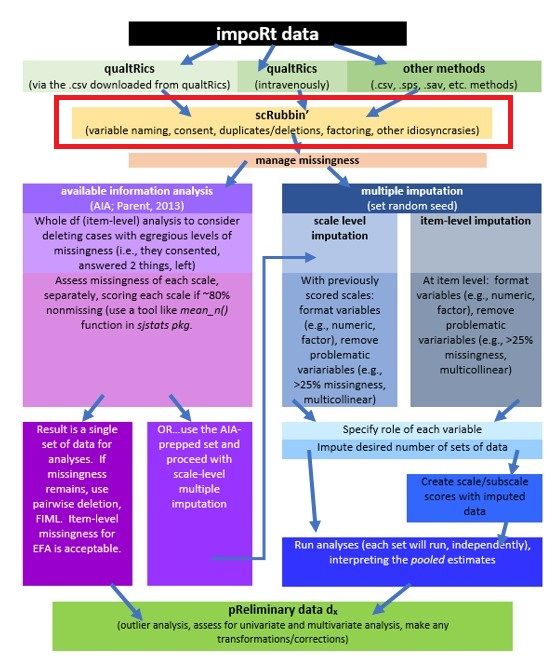
\includegraphics{images/Ch02/wrkflow_prelim.jpg}
\caption{An image of our stage in the workflow for scrubbing and scoring data.}
\end{figure}

\hypertarget{research-vignette-1}{%
\section{Research Vignette}\label{research-vignette-1}}

The research vignette comes from the survey titled, \href{https://spupsych.az1.qualtrics.com/jfe/form/SV_b2cClqAlLGQ6nLU}{Rate-a-Recent-Course: A ReCentering Psych Stats Exercise} and is explained in the prior chapter. In the prior chapter we conducted super-preliminary scrubbing of variables that will allow us to examine the respondent's perceived campus climate for students who are Black, predicted by the the respondent's own campus belonging, and also the \emph{structural diversity} proportions of Black students in the classroom and the BIPOC instructional staff. At present, I see this as a parallel mediation. That is, the perceived campus climate for Black students will be predicted by the respondent's sense of belonging, through the proportion of Black classmates and BIPOC (Black, Indigenous, and people of color)instructional staff.

\emph{I would like to assess the model by having the instructional staff variable to be the percent of Black instructional staff. At the time that this lecture is being prepared, there is insufficient representation of Black faculty to model this.}

\begin{figure}
\centering
\includegraphics{images/Ch03/BlStuMed.jpg}
\caption{An image of the statistical model for which we are preparing data.}
\end{figure}

First, though, let's take a more conceptual look at issues regarding missing data. We'll come back to details of the survey as we work with it.

\hypertarget{on-missing-data}{%
\section{On Missing Data}\label{on-missing-data}}

On the topic of missing data, we follow the traditions in most textbooks. We start by considering \emph{data loss mechanisms} and options for \emph{managing missingness.}

Although the workflow I recommend is fairly straightforward, the topic is not. Quantitative psychologist have produced volumes of research that supports and refutes all of these issues in detail. An in-deth review of this is found in Enders' \citeyearpar{enders_applied_2010} text.

\hypertarget{data-loss-mechanisms}{%
\subsection{Data Loss Mechanisms}\label{data-loss-mechanisms}}

We generally classify missingess in data in three different ways \citep{kline_principles_2016, parent_handling_2013}:

\textbf{Missing completely at random (MCAR)} is the ideal case (and often unrealistic in actual data). For variable \emph{Y} this mean that

\begin{itemize}
\tightlist
\item
  Missingness is due to a factor(s) completely unrelated to the missing data. Stated another way:

  \begin{itemize}
  \tightlist
  \item
    Missing observations differ from the observed scores only by chance; that is, whether scores on Y are missing or not missing is unrelated to \emph{Y} itself
  \end{itemize}
\item
  The presence versus absence of data on \emph{Y} is unrelated to all other variables in the dataset. That is, the nonmissing data are just a random sample of scores that the researcher would have analyzed had the data been complete. We might think of it as \emph{haphazard} missing.

  \begin{itemize}
  \tightlist
  \item
    A respondent is interrupted, looks up, looks down, and skips an item.
  \item
    A computer glitch causes spotty missingness -- unrelated to any particular variable.
  \end{itemize}
\end{itemize}

MCAR is the ideal state because results from it should not be biased as a function of the missingness.

\textbf{Missing at random (MAR)} missing data arise from a process that is both measured and predictable in a particular sample. \emph{Admittedly the use of ``random'' in this term is odd, because, by definition, the missingness is not random.}

Restated:

\begin{enumerate}
\def\labelenumi{\arabic{enumi}.}
\tightlist
\item
  Missingness on Y is unrelated to Y itself, but
\item
  Missingness is on Y is correlated with other variables in the data set.
\end{enumerate}

Example: Men are less likely to respond to questions about mental health than women, but among men, the probability of responding is unrelated to their true mental health status.

Kline \citeyearpar{kline_principles_2016} indicated that information loss due to MAR is potentially recoverable through imputation where missing scores are replaced by predicted scores. The predicted scores are generated from other variables in the data set that predict missingness on Y. If the strength of that prediction is reasonably strong, then results on Y after imputation may be relatively unbiased. In this sense, the MAR pattern is described as \emph{ignorable} with regard to potential bias. Two types of variables can be used to predict the missing data

\begin{enumerate}
\def\labelenumi{\arabic{enumi}.}
\tightlist
\item
  variables that are in the prediction equation, and
\item
  \emph{auxiliary} variables (i.e., variables in the dataset that are not in the prediction equation).
\end{enumerate}

Parent \citeyearpar{parent_handling_2013} noted that multiple imputation and expectation maximization have frequently been used to manage missingness in MAR circumstances.

\textbf{Missing not at random (MNAR)} is when the presence versus absence of scores on \emph{Y} depend on \emph{Y} itself. This is \emph{non-ignorable}.

For example, if a patient drops out of a medical RCT because there are unpleasant side effects from the treatment, this discomfort is not measured, but the data is missing due to a process that is unknown in a particular data set. Results based on \emph{complete cases only} can be severely biased when the data loss pattern is MNAR. That is, a treatment may look more beneficial than it really is if data from patients who were unable to tolerate the treatment are lost.

Parent \citeyearpar{parent_handling_2013} described MNAR a little differently -- but emphasized that the systematic missingness would be related to a variable outside the datset. Parent provided the example of items written in a manner that may be inappropriate for some participants (e.g., asking women about a relationship with their boyfriend/husband, when the woman might be in same gender relationship). If there were not demographic items that could identify the bias, this would be MNAR. Parent strongly advises researchers to carefully proofread and pilot surveys to avoid MNAR circumstances.

Kline \citeyearpar{kline_principles_2016} noted that the choice of the method to deal with the incomplete records can make a difference in the results, and should be made carefully.

\hypertarget{diagnosing-missing-data-mechanisms}{%
\subsection{Diagnosing Missing Data Mechanisms}\label{diagnosing-missing-data-mechanisms}}

The bad news is that we never really know (with certainty) the type of missing data mechanism in our data. The following tools can help understand the mechanisms that contribute to missingness.

\begin{itemize}
\tightlist
\item
  Missing data analyses often includes correlations that could predict missingness.
\item
  Little and Rubin \citeyearpar{little_statistical_2002} proposed a multivariate statistical test of the MCAR assumption that simultaneously compares complete versus incomplete cases on \emph{Y} across all other variables. If this comparison is significant, then the MCAR hypothesis is rejected.

  \begin{itemize}
  \tightlist
  \item
    To restate: we want a non-significant result; and we use the sometimes-backwards-sounding NHST (null hypothesis significance testing) language, ``MCAR cannot be rejected.''
  \end{itemize}
\item
  MCAR can also be examined through a series of \emph{t} tests of the cases that have missing scores on Y with cases that have complete records on other variables. Unfortunately, sample sizes contribute to problems with interpretation. With low samples, they are underpowered; in large samples they can flag trivial differences.
\end{itemize}

If MCAR is rejected, we are never sure whether the data loss mechanism is MAR or MNAR. There is no magical statistical ``fix.'' Kline \citeyearpar{kline_principles_2016} wrote, ``About the best that can be done is to understand the nature of the underlying data loss pattern and accordingly modify your interpretation of the results'' (p.~85).

\hypertarget{managing-missing-data}{%
\subsection{Managing Missing Data}\label{managing-missing-data}}

There are a number of approaches to managing missing data. Here is a summary of the ones most commonly used.

\begin{itemize}
\item
  \textbf{Listwise deletion} (aka, Complete Case Analysis) If there is a missing score on any variable, that case is excluded from \textbf{all} analyses.
\item
  \textbf{Pairwise deletion} Cases are excluded only if they have missing data on variables involved in a particular analysis. AIA is a variant of pair-wise deletion, but it preserves as much data as possible with person-mean imputation at the scale level.
\item
  \textbf{Mean/median substitution} Mean/median substitution replaces missing values with the mean/median of that particular variable. While this preserves the mean of the dataset, it can cause bias by decreasing variance. For example, if you have a column that has substantial of missingness and you replace each value with the same, fixed, mean, the variability of that variable has just been reduced. A variation on this is a \textbf{group-mean substitution} where the missing score in a particular group (e.g., women) is replaced by the group mean.
\item
  \textbf{Full information maximum likelihood (FIML)} A \emph{model-based method} that takes the researcher's model as the starting point. The procedure partitions the cases in a raw data file into subsets, each with the same pattern of missing observations, including none (complete cases). Statistical information (e.g., means, variances) is extracted from each subset so all case are retained in the analysis. Parameters for the researcher's model are estimated after combining all available information over the subsets of cases.
\item
  \textbf{Multiple imputation} A \emph{data based method} that works with the whole raw data file (not just with the observed variables that comprise the researcher's model). Multiple imputation assumes that data are MAR (remember, MCAR is the more prestigious one). This means that researchers assume that missing values can be replaced by predictions derived from the observable portion fo the dataset.

  \begin{itemize}
  \tightlist
  \item
    Multiple datasets (often 5 to 20) are created where missing values are replaced via a randomized process (so the same missing value {[}item 4 for person A{]} will likely have different values for each dataset).
  \item
    The desired anlayis(es) is conducted simultaneously/separately for each of the imputed sets (so if you imputed 5 sets and wanted a linear regression, you get 5 linear regressions).
  \item
    A \emph{pooled analysis} uses the point estimates and the standard errors to provide a single result that represents the analysis.
  \end{itemize}
\end{itemize}

\hypertarget{available-information-analysis-aia}{%
\subsection{Available Information Analysis (AIA)}\label{available-information-analysis-aia}}

Parent \citeyearpar{parent_handling_2013} has created a set of recommendations that help us create a streamlined workflow for managing missing data. After evaluating three approaches to managing missingness (AIA, mean substitution, and multiple imputation) Parent concluded that in datasets with (a) low levels of missingness, (b) a reasonable sample size, and (c) adequate internal reliability of measures, these approaches had similar results.

Further, in simulation studies where there was (a) low sample size (\emph{n} = 50), (b) weak associations among items, and (c) a small number of missing items, AIA was equivalent to multiple imputation. Even in cases where the data conditions were the ``best'' (i.e., \emph{N} = 200, moderate correlations, at least 10 items), even 10\% missingness (overall) did not produce notable difference among the methods. That is, means, standard errors, and alphas were similar across the methods (AIA, mean substitution, multiple imputation).

AIA is an older method of handling missing data that, as its name suggests, uses the \emph{available data} for analysis and excludes missing data points only for analyses in which the missing data point would be directly involved. This means

\begin{itemize}
\tightlist
\item
  In the case of research that uses multiple item scales, and analysis takes place at the scale level

  \begin{itemize}
  \tightlist
  \item
    AIA is used to generate \textbf{mean} scores for the scale using the available data without substituting or imputing values;
  \item
    This method generally produces a fairly complete set of scale-level data where

    \begin{itemize}
    \tightlist
    \item
      pairwise deletion (the whole row/case/person is skipped) can be used where there will be multiple analyses using statistics (e.g., correlations, t-tests, ANOVA) were missingness is not permitted
    \item
      FIML can be specified in path analysis and CFA/SEM (where item-level data is required), and
    \item
      some statistics, such as principal components analysis and principal axis factoring (item-level analyses) permit missing data,
    \end{itemize}
  \item
    Of course, the researcher could still impute data, but why\ldots{}
  \end{itemize}
\end{itemize}

Parent's \citeyearpar{parent_handling_2013} recommendations:

\begin{itemize}
\tightlist
\item
  Scale scores should be first calculated as a \emph{mean} (average) not a sum. Why?

  \begin{itemize}
  \tightlist
  \item
    Calculating a ``sum'' from available data will result in automatically lower scores in cases where there is missingness.
  \item
    If a sum is required (i.e., because you want to interpret some clinical level of something), calculate the mean first, do the analyses, then transform the results back into the whole-scale equivalent (multiply the mean by the number of items) for any interpretation.
  \item
    For R script, do not write the script ({[}item1 + item2 + item3{]}/3) because this will return an empty entry for participants missing data (same problem as if you were to use sum). There are several functions for properly computing a mean; I will demo the \emph{mean\_n()} function from \emph{sjstats} package because it allows us to simultaneously specify the tolerance level (next item).
  \end{itemize}
\item
  Determine your \emph{tolerance} for missingness (20\% seems to be common, although you could also look for guidance in the test manual/article). Then

  \begin{itemize}
  \tightlist
  \item
    Run a ``percent missingness'' check on the level of analysis (i.e., total score, scale, or subscale) you are using. If you are using a total scale score, then check to see what percent is missing across all the items in the whole scale. In contrast, if you are looking at subscales, run the percent missing at that level.
  \item
    Parent \citeyearpar{parent_handling_2013} advised that the tolerance levels should be made mindfully. A four-item scale with one item missing, won't meet the 80\% threshold, so it may make sense to set a 75\% threshold for this scale.
  \end{itemize}
\item
  ``Clearly and concisely detail the level of missingness'' in papers \citep[p.~595]{parent_handling_2013}. This includes

  \begin{itemize}
  \tightlist
  \item
    tolerance level for missing data by scale or subscale (e.g., 80\% or 75\%)
  \item
    the number of missing values out of all data points on that scale for all participants and the maximum by participant (e.g., ``For Scale X, a total of \# missing data points out of \#\#\# were observed with no participant missing more than a single point.'')
  \item
    verify a manual inspection of missing data for obvious patterns (e.g., abnormally high missing rates for only one or two items). This can be accomplished by requesting frequency output for the items and checking the nonmissing data points for each scale, ensuring there are no abnormal spikes in missingness (looking for MNAR).
  \end{itemize}
\item
  Curiously, Parent \citeyearpar{parent_handling_2013} does not recommend that we run all the diagnostic tests. However, because recent reviewers have required them of me, I will demonstrate a series of them.
\item
  Reducing missingness starts at the survey design -- make sure that all people can answer all items (i.e,. relationship-related items may contain heterosexist assumptions\ldots which would result in an MNAR circumstance)
\end{itemize}

Very practically speaking, Parent's \citeyearpar{parent_handling_2013} recommendations follow us through the entire data analysis process.

\hypertarget{working-the-problem-1}{%
\section{Working the Problem}\label{working-the-problem-1}}

\hypertarget{variable-planning-and-preparation}{%
\subsection{Variable Planning and Preparation}\label{variable-planning-and-preparation}}

In the \protect\hyperlink{scrub}{Scrubbing lesson} we imported the data from Qualtrics and applied the broadest levels of inclusion (e.g., the course rated was offered from an institution in the U.S., the respondent consented to participation) and exclusion (e.g., the survey was not a preview). We then downsized the survey to include the variables we will use in our statistical model. We then saved the data in .csv and .rds file.

Presuming that you are working along with me in an .rmd file and have placed that file in the same folder as this .rmd file, the following code should read the data into your environment.

I use \emph{different} names for the object/df in my R environment than I use for the filename that holds the data on my computer. Why? I don't want to accidentally overwrite this precious ``source'' of data.

\begin{Shaded}
\begin{Highlighting}[]
\CommentTok{\# scrub\_df \textless{}{-} read.csv (\textquotesingle{}BlackStntsModel230902.csv\textquotesingle{}, head = TRUE, sep}
\CommentTok{\# = \textquotesingle{},\textquotesingle{})}
\NormalTok{scrub\_df }\OtherTok{\textless{}{-}} \FunctionTok{readRDS}\NormalTok{(}\StringTok{"BlackStntsModel230902.rds"}\NormalTok{)}
\FunctionTok{str}\NormalTok{(scrub\_df)}
\end{Highlighting}
\end{Shaded}

\begin{verbatim}
## Classes 'tbl_df', 'tbl' and 'data.frame':    69 obs. of  25 variables:
##  $ ID       : int  1 2 3 4 5 6 7 8 9 10 ...
##  $ iRace1   : num  3 3 3 3 1 3 3 3 1 0 ...
##   ..- attr(*, "label")= Named chr "1 - From your perspective as a student, which of the following best describes the [Field-2] instructor."
##   .. ..- attr(*, "names")= chr "1_iRace"
##  $ iRace2   : num  1 NA 1 1 NA NA 3 NA NA 0 ...
##   ..- attr(*, "label")= Named chr "2 - From your perspective as a student, which of the following best describes the [Field-2] instructor."
##   .. ..- attr(*, "names")= chr "2_iRace"
##  $ iRace3   : num  3 NA NA 3 NA NA NA NA NA 3 ...
##   ..- attr(*, "label")= Named chr "3 - From your perspective as a student, which of the following best describes the [Field-2] instructor."
##   .. ..- attr(*, "names")= chr "3_iRace"
##  $ iRace4   : num  NA NA NA NA NA NA NA NA NA 3 ...
##   ..- attr(*, "label")= Named chr "4 - From your perspective as a student, which of the following best describes the [Field-2] instructor."
##   .. ..- attr(*, "names")= chr "4_iRace"
##  $ iRace5   : logi  NA NA NA NA NA NA ...
##   ..- attr(*, "label")= Named chr "5 - From your perspective as a student, which of the following best describes the [Field-2] instructor."
##   .. ..- attr(*, "names")= chr "5_iRace"
##  $ iRace6   : logi  NA NA NA NA NA NA ...
##   ..- attr(*, "label")= Named chr "6 - From your perspective as a student, which of the following best describes the [Field-2] instructor."
##   .. ..- attr(*, "names")= chr "6_iRace"
##  $ iRace7   : logi  NA NA NA NA NA NA ...
##   ..- attr(*, "label")= Named chr "7 - From your perspective as a student, which of the following best describes the [Field-2] instructor."
##   .. ..- attr(*, "names")= chr "7_iRace"
##  $ iRace8   : logi  NA NA NA NA NA NA ...
##   ..- attr(*, "label")= Named chr "8 - From your perspective as a student, which of the following best describes the [Field-2] instructor."
##   .. ..- attr(*, "names")= chr "8_iRace"
##  $ iRace9   : logi  NA NA NA NA NA NA ...
##   ..- attr(*, "label")= Named chr "9 - From your perspective as a student, which of the following best describes the [Field-2] instructor."
##   .. ..- attr(*, "names")= chr "9_iRace"
##  $ iRace10  : logi  NA NA NA NA NA NA ...
##   ..- attr(*, "label")= Named chr "10 - From your perspective as a student, which of the following best describes the [Field-2] instructor."
##   .. ..- attr(*, "names")= chr "10_iRace"
##  $ cmBiMulti: num  0 0 0 2 5 15 0 0 0 7 ...
##   ..- attr(*, "label")= Named chr "Regarding race, what proportion of students were from each broad classification.  Your responses should add to "| __truncated__
##   .. ..- attr(*, "names")= chr "Race_10"
##  $ cmBlack  : num  0 5 10 6 5 20 0 0 0 4 ...
##   ..- attr(*, "label")= Named chr "Regarding race, what proportion of students were from each broad classification.  Your responses should add to 100%. - Black"
##   .. ..- attr(*, "names")= chr "Race_1"
##  $ cmNBPoC  : num  39 10 30 19 10 30 40 5 30 13 ...
##   ..- attr(*, "label")= Named chr "Regarding race, what proportion of students were from each broad classification.  Your responses should add to "| __truncated__
##   .. ..- attr(*, "names")= chr "Race_7"
##  $ cmWhite  : num  61 85 60 73 80 35 60 90 70 73 ...
##   ..- attr(*, "label")= Named chr "Regarding race, what proportion of students were from each broad classification.  Your responses should add to 100%. - White"
##   .. ..- attr(*, "names")= chr "Race_8"
##  $ cmUnsure : num  0 0 0 0 0 0 0 5 0 3 ...
##   ..- attr(*, "label")= Named chr "Regarding race, what proportion of students were from each broad classification.  Your responses should add to 100%. - Unsure"
##   .. ..- attr(*, "names")= chr "Race_2"
##  $ Belong_1 : num  6 4 NA 5 4 5 6 7 6 3 ...
##   ..- attr(*, "label")= Named chr "Please indicate the degree to which you agree with the following questions about the course. Please skip the it"| __truncated__
##   .. ..- attr(*, "names")= chr "Belong_1"
##  $ Belong_2 : num  6 4 3 3 4 6 6 7 6 3 ...
##   ..- attr(*, "label")= Named chr "Please indicate the degree to which you agree with the following questions about the course. Please skip the it"| __truncated__
##   .. ..- attr(*, "names")= chr "Belong_2"
##  $ Belong_3 : num  7 6 NA 2 4 5 5 7 6 3 ...
##   ..- attr(*, "label")= Named chr "Please indicate the degree to which you agree with the following questions about the course. Please skip the it"| __truncated__
##   .. ..- attr(*, "names")= chr "Belong_3"
##  $ Blst_1   : num  5 6 NA 2 6 5 5 5 5 3 ...
##   ..- attr(*, "label")= Named chr "Each item below asks you to rate elements of campus climate for your \"academic department/program.\"  If you d"| __truncated__
##   .. ..- attr(*, "names")= chr "Blst_1"
##  $ Blst_2   : num  3 6 5 2 1 1 4 4 3 5 ...
##   ..- attr(*, "label")= Named chr "Each item below asks you to rate elements of campus climate for your \"academic department/program.\"  If you d"| __truncated__
##   .. ..- attr(*, "names")= chr "Blst_2"
##  $ Blst_3   : num  5 2 2 2 1 1 4 3 1 2 ...
##   ..- attr(*, "label")= Named chr "Each item below asks you to rate elements of campus climate for your \"academic department/program.\"  If you d"| __truncated__
##   .. ..- attr(*, "names")= chr "Blst_3"
##  $ Blst_4   : num  2 2 2 2 1 2 4 3 2 3 ...
##   ..- attr(*, "label")= Named chr "Each item below asks you to rate elements of campus climate for your \"academic department/program.\"  If you d"| __truncated__
##   .. ..- attr(*, "names")= chr "Blst_4"
##  $ Blst_5   : num  2 4 NA 2 1 1 4 4 1 3 ...
##   ..- attr(*, "label")= Named chr "Each item below asks you to rate elements of campus climate for your \"academic department/program.\"  If you d"| __truncated__
##   .. ..- attr(*, "names")= chr "Blst_5"
##  $ Blst_6   : num  2 1 2 2 1 2 4 3 2 3 ...
##   ..- attr(*, "label")= Named chr "Each item below asks you to rate elements of campus climate for your \"academic department/program.\"  If you d"| __truncated__
##   .. ..- attr(*, "names")= chr "Blst_6"
##  - attr(*, "column_map")=Classes 'tbl_df', 'tbl' and 'data.frame':   182 obs. of  7 variables:
##   ..$ qname      : chr [1:182] "StartDate" "EndDate" "Status" "Progress" ...
##   ..$ description: chr [1:182] "Start Date" "End Date" "Response Type" "Progress" ...
##   ..$ main       : chr [1:182] "Start Date" "End Date" "Response Type" "Progress" ...
##   ..$ sub        : chr [1:182] "" "" "" "" ...
##   ..$ ImportId   : chr [1:182] "startDate" "endDate" "status" "progress" ...
##   ..$ timeZone   : chr [1:182] "America/Los_Angeles" "America/Los_Angeles" NA NA ...
##   ..$ choiceId   : chr [1:182] NA NA NA NA ...
\end{verbatim}

Let's think about how the variables in our model should be measured:

\begin{itemize}
\tightlist
\item
  DV: Campus Climate for Black Students (as perceived by the respondent)

  \begin{itemize}
  \tightlist
  \item
    mean score of the 6 items on that scale (higher scores indicate a climate characterized by hostility, nonresponsiveness, and stigma)
  \item
    1 item needs to be reverse-coded
  \item
    this scale was adapted from the LGBT Campus Climate Scale \citep{szymanski_perceptions_2020}
  \end{itemize}
\item
  IV: Belonging

  \begin{itemize}
  \tightlist
  \item
    mean score for the 3 items on that scale (higher scores indicate a greater sense of belonging)
  \item
    this scale is taken from the Sense of Belonging subscale from the Perceived Cohesion Scale \citep{bollen_perceived_1990}
  \end{itemize}
\item
  Proportion of classmates who are Black

  \begin{itemize}
  \tightlist
  \item
    a single item
  \end{itemize}
\item
  Proportion of instructional staff who are BIPOC

  \begin{itemize}
  \tightlist
  \item
    must be calculated from each of the single items for each instructor
  \end{itemize}
\end{itemize}

To summarize, the Campus Climate and Belonging scales are traditional in the sense that they have items that we sum. The variable representing proportion of classmates who are Black is a single item. The variable representing the proportion of instructional staff who are BIPOC must be calculated in a manner that takes into consideration the there may be multiple instructors. The survey allowed a respondent to name up to 10 instructors.

\begin{Shaded}
\begin{Highlighting}[]
\FunctionTok{str}\NormalTok{(scrub\_df}\SpecialCharTok{$}\NormalTok{iRace1)}
\end{Highlighting}
\end{Shaded}

\begin{verbatim}
##  num [1:69] 3 3 3 3 1 3 3 3 1 0 ...
##  - attr(*, "label")= Named chr "1 - From your perspective as a student, which of the following best describes the [Field-2] instructor."
##   ..- attr(*, "names")= chr "1_iRace"
\end{verbatim}

Looking at the structure of our data, the iRace(1 thru 10) variables are in ``int'' or integer format. This means that they are represented as whole numbers. We need them to be represented as factors. R handles factors represented as words well. Therefore, let's use our codebook to reformat this variable as a an ordered factor, with words instead of numbers.

Qualtrics imports many of the categorical variables as numbers. R often reads them numerically (integers or numbers). If they are directly converted to factors, R will sometimes collapse across missing numbers. In this example, if there is a race that is not represented (e.g., 2 for BiMulti), when the numbers are changed to factors, R will assume they are ordered and there is a consecutive series of numbers (0,1,2,3,4). If a number in the sequence is missing (0,1,3,4) and labels are applied, it will collapse across the numbers and the labels you think are attached to each number are not. Therefore, it is ESSENTIAL to check (again and again ad nauseum) to ensure that your variables are recoding in a manner you understand.

One way to avoid this is to use the code below to identify the levels and the labels. When they are in order, they align and don't ``skip'' numbers. To quadruple check our work, we will recode into a new variable ``tRace\#'' for ``teacher'' Race.

\begin{Shaded}
\begin{Highlighting}[]
\NormalTok{scrub\_df}\SpecialCharTok{$}\NormalTok{tRace1 }\OtherTok{=} \FunctionTok{factor}\NormalTok{(scrub\_df}\SpecialCharTok{$}\NormalTok{iRace1, }\AttributeTok{levels =} \FunctionTok{c}\NormalTok{(}\DecValTok{0}\NormalTok{, }\DecValTok{1}\NormalTok{, }\DecValTok{2}\NormalTok{, }\DecValTok{3}\NormalTok{, }\DecValTok{4}\NormalTok{), }\AttributeTok{labels =} \FunctionTok{c}\NormalTok{(}\StringTok{"Black"}\NormalTok{,}
    \StringTok{"nBpoc"}\NormalTok{, }\StringTok{"BiMulti"}\NormalTok{, }\StringTok{"White"}\NormalTok{, }\StringTok{"NotNotice"}\NormalTok{))}
\NormalTok{scrub\_df}\SpecialCharTok{$}\NormalTok{tRace2 }\OtherTok{=} \FunctionTok{factor}\NormalTok{(scrub\_df}\SpecialCharTok{$}\NormalTok{iRace2, }\AttributeTok{levels =} \FunctionTok{c}\NormalTok{(}\DecValTok{0}\NormalTok{, }\DecValTok{1}\NormalTok{, }\DecValTok{2}\NormalTok{, }\DecValTok{3}\NormalTok{, }\DecValTok{4}\NormalTok{), }\AttributeTok{labels =} \FunctionTok{c}\NormalTok{(}\StringTok{"Black"}\NormalTok{,}
    \StringTok{"nBpoc"}\NormalTok{, }\StringTok{"BiMulti"}\NormalTok{, }\StringTok{"White"}\NormalTok{, }\StringTok{"NotNotice"}\NormalTok{))}
\NormalTok{scrub\_df}\SpecialCharTok{$}\NormalTok{tRace3 }\OtherTok{=} \FunctionTok{factor}\NormalTok{(scrub\_df}\SpecialCharTok{$}\NormalTok{iRace3, }\AttributeTok{levels =} \FunctionTok{c}\NormalTok{(}\DecValTok{0}\NormalTok{, }\DecValTok{1}\NormalTok{, }\DecValTok{2}\NormalTok{, }\DecValTok{3}\NormalTok{, }\DecValTok{4}\NormalTok{), }\AttributeTok{labels =} \FunctionTok{c}\NormalTok{(}\StringTok{"Black"}\NormalTok{,}
    \StringTok{"nBpoc"}\NormalTok{, }\StringTok{"BiMulti"}\NormalTok{, }\StringTok{"White"}\NormalTok{, }\StringTok{"NotNotice"}\NormalTok{))}
\NormalTok{scrub\_df}\SpecialCharTok{$}\NormalTok{tRace4 }\OtherTok{=} \FunctionTok{factor}\NormalTok{(scrub\_df}\SpecialCharTok{$}\NormalTok{iRace4, }\AttributeTok{levels =} \FunctionTok{c}\NormalTok{(}\DecValTok{0}\NormalTok{, }\DecValTok{1}\NormalTok{, }\DecValTok{2}\NormalTok{, }\DecValTok{3}\NormalTok{, }\DecValTok{4}\NormalTok{), }\AttributeTok{labels =} \FunctionTok{c}\NormalTok{(}\StringTok{"Black"}\NormalTok{,}
    \StringTok{"nBpoc"}\NormalTok{, }\StringTok{"BiMulti"}\NormalTok{, }\StringTok{"White"}\NormalTok{, }\StringTok{"NotNotice"}\NormalTok{))}
\NormalTok{scrub\_df}\SpecialCharTok{$}\NormalTok{tRace5 }\OtherTok{=} \FunctionTok{factor}\NormalTok{(scrub\_df}\SpecialCharTok{$}\NormalTok{iRace5, }\AttributeTok{levels =} \FunctionTok{c}\NormalTok{(}\DecValTok{0}\NormalTok{, }\DecValTok{1}\NormalTok{, }\DecValTok{2}\NormalTok{, }\DecValTok{3}\NormalTok{, }\DecValTok{4}\NormalTok{), }\AttributeTok{labels =} \FunctionTok{c}\NormalTok{(}\StringTok{"Black"}\NormalTok{,}
    \StringTok{"nBpoc"}\NormalTok{, }\StringTok{"BiMulti"}\NormalTok{, }\StringTok{"White"}\NormalTok{, }\StringTok{"NotNotice"}\NormalTok{))}
\NormalTok{scrub\_df}\SpecialCharTok{$}\NormalTok{tRace6 }\OtherTok{=} \FunctionTok{factor}\NormalTok{(scrub\_df}\SpecialCharTok{$}\NormalTok{iRace6, }\AttributeTok{levels =} \FunctionTok{c}\NormalTok{(}\DecValTok{0}\NormalTok{, }\DecValTok{1}\NormalTok{, }\DecValTok{2}\NormalTok{, }\DecValTok{3}\NormalTok{, }\DecValTok{4}\NormalTok{), }\AttributeTok{labels =} \FunctionTok{c}\NormalTok{(}\StringTok{"Black"}\NormalTok{,}
    \StringTok{"nBpoc"}\NormalTok{, }\StringTok{"BiMulti"}\NormalTok{, }\StringTok{"White"}\NormalTok{, }\StringTok{"NotNotice"}\NormalTok{))}
\NormalTok{scrub\_df}\SpecialCharTok{$}\NormalTok{tRace7 }\OtherTok{=} \FunctionTok{factor}\NormalTok{(scrub\_df}\SpecialCharTok{$}\NormalTok{iRace7, }\AttributeTok{levels =} \FunctionTok{c}\NormalTok{(}\DecValTok{0}\NormalTok{, }\DecValTok{1}\NormalTok{, }\DecValTok{2}\NormalTok{, }\DecValTok{3}\NormalTok{, }\DecValTok{4}\NormalTok{), }\AttributeTok{labels =} \FunctionTok{c}\NormalTok{(}\StringTok{"Black"}\NormalTok{,}
    \StringTok{"nBpoc"}\NormalTok{, }\StringTok{"BiMulti"}\NormalTok{, }\StringTok{"White"}\NormalTok{, }\StringTok{"NotNotice"}\NormalTok{))}
\NormalTok{scrub\_df}\SpecialCharTok{$}\NormalTok{tRace8 }\OtherTok{=} \FunctionTok{factor}\NormalTok{(scrub\_df}\SpecialCharTok{$}\NormalTok{iRace8, }\AttributeTok{levels =} \FunctionTok{c}\NormalTok{(}\DecValTok{0}\NormalTok{, }\DecValTok{1}\NormalTok{, }\DecValTok{2}\NormalTok{, }\DecValTok{3}\NormalTok{, }\DecValTok{4}\NormalTok{), }\AttributeTok{labels =} \FunctionTok{c}\NormalTok{(}\StringTok{"Black"}\NormalTok{,}
    \StringTok{"nBpoc"}\NormalTok{, }\StringTok{"BiMulti"}\NormalTok{, }\StringTok{"White"}\NormalTok{, }\StringTok{"NotNotice"}\NormalTok{))}
\NormalTok{scrub\_df}\SpecialCharTok{$}\NormalTok{tRace9 }\OtherTok{=} \FunctionTok{factor}\NormalTok{(scrub\_df}\SpecialCharTok{$}\NormalTok{iRace9, }\AttributeTok{levels =} \FunctionTok{c}\NormalTok{(}\DecValTok{0}\NormalTok{, }\DecValTok{1}\NormalTok{, }\DecValTok{2}\NormalTok{, }\DecValTok{3}\NormalTok{, }\DecValTok{4}\NormalTok{), }\AttributeTok{labels =} \FunctionTok{c}\NormalTok{(}\StringTok{"Black"}\NormalTok{,}
    \StringTok{"nBpoc"}\NormalTok{, }\StringTok{"BiMulti"}\NormalTok{, }\StringTok{"White"}\NormalTok{, }\StringTok{"NotNotice"}\NormalTok{))}
\NormalTok{scrub\_df}\SpecialCharTok{$}\NormalTok{tRace10 }\OtherTok{=} \FunctionTok{factor}\NormalTok{(scrub\_df}\SpecialCharTok{$}\NormalTok{iRace10, }\AttributeTok{levels =} \FunctionTok{c}\NormalTok{(}\DecValTok{0}\NormalTok{, }\DecValTok{1}\NormalTok{, }\DecValTok{2}\NormalTok{, }\DecValTok{3}\NormalTok{, }\DecValTok{4}\NormalTok{),}
    \AttributeTok{labels =} \FunctionTok{c}\NormalTok{(}\StringTok{"Black"}\NormalTok{, }\StringTok{"nBpoc"}\NormalTok{, }\StringTok{"BiMulti"}\NormalTok{, }\StringTok{"White"}\NormalTok{, }\StringTok{"NotNotice"}\NormalTok{))}
\end{Highlighting}
\end{Shaded}

Let's check the structure to see if they are factors.

\begin{Shaded}
\begin{Highlighting}[]
\FunctionTok{library}\NormalTok{(tidyverse)}
\end{Highlighting}
\end{Shaded}

\begin{verbatim}
## -- Attaching core tidyverse packages ------------------------ tidyverse 2.0.0 --
## v dplyr     1.1.2     v readr     2.1.4
## v forcats   1.0.0     v stringr   1.5.0
## v ggplot2   3.4.3     v tibble    3.2.1
## v lubridate 1.9.2     v tidyr     1.3.0
## v purrr     1.0.1     
## -- Conflicts ------------------------------------------ tidyverse_conflicts() --
## x dplyr::filter() masks stats::filter()
## x dplyr::lag()    masks stats::lag()
## i Use the conflicted package (<http://conflicted.r-lib.org/>) to force all conflicts to become errors
\end{verbatim}

\begin{Shaded}
\begin{Highlighting}[]
\FunctionTok{glimpse}\NormalTok{(scrub\_df)}
\end{Highlighting}
\end{Shaded}

\begin{verbatim}
## Rows: 69
## Columns: 35
## $ ID        <int> 1, 2, 3, 4, 5, 6, 7, 8, 9, 10, 11, 12, 13, 14, 15, 16, 17, 1~
## $ iRace1    <dbl> 3, 3, 3, 3, 1, 3, 3, 3, 1, 0, 2, 1, 1, 1, 3, 3, 3, 1, 3, 3, ~
## $ iRace2    <dbl> 1, NA, 1, 1, NA, NA, 3, NA, NA, 0, NA, NA, 3, NA, 3, 3, NA, ~
## $ iRace3    <dbl> 3, NA, NA, 3, NA, NA, NA, NA, NA, 3, NA, NA, NA, NA, 3, 1, N~
## $ iRace4    <dbl> NA, NA, NA, NA, NA, NA, NA, NA, NA, 3, NA, NA, NA, NA, NA, 3~
## $ iRace5    <lgl> NA, NA, NA, NA, NA, NA, NA, NA, NA, NA, NA, NA, NA, NA, NA, ~
## $ iRace6    <lgl> NA, NA, NA, NA, NA, NA, NA, NA, NA, NA, NA, NA, NA, NA, NA, ~
## $ iRace7    <lgl> NA, NA, NA, NA, NA, NA, NA, NA, NA, NA, NA, NA, NA, NA, NA, ~
## $ iRace8    <lgl> NA, NA, NA, NA, NA, NA, NA, NA, NA, NA, NA, NA, NA, NA, NA, ~
## $ iRace9    <lgl> NA, NA, NA, NA, NA, NA, NA, NA, NA, NA, NA, NA, NA, NA, NA, ~
## $ iRace10   <lgl> NA, NA, NA, NA, NA, NA, NA, NA, NA, NA, NA, NA, NA, NA, NA, ~
## $ cmBiMulti <dbl> 0, 0, 0, 2, 5, 15, 0, 0, 0, 7, 0, 0, 20, 0, 9, 12, 0, 6, 6, ~
## $ cmBlack   <dbl> 0, 5, 10, 6, 5, 20, 0, 0, 0, 4, 0, 7, 0, 6, 9, 1, 21, 5, 6, ~
## $ cmNBPoC   <dbl> 39, 10, 30, 19, 10, 30, 40, 5, 30, 13, 80, 19, 0, 19, 15, 22~
## $ cmWhite   <dbl> 61, 85, 60, 73, 80, 35, 60, 90, 70, 73, 10, 74, 80, 0, 67, 5~
## $ cmUnsure  <dbl> 0, 0, 0, 0, 0, 0, 0, 5, 0, 3, 10, 0, 0, 75, 0, 14, 0, 5, 0, ~
## $ Belong_1  <dbl> 6, 4, NA, 5, 4, 5, 6, 7, 6, 3, 6, 6, 3, 4, 3, 3, 4, 5, 1, 2,~
## $ Belong_2  <dbl> 6, 4, 3, 3, 4, 6, 6, 7, 6, 3, 6, 6, 5, 4, 3, 3, 4, 6, 1, 2, ~
## $ Belong_3  <dbl> 7, 6, NA, 2, 4, 5, 5, 7, 6, 3, 5, 6, 4, 4, 3, 2, 4, 5, 1, 1,~
## $ Blst_1    <dbl> 5, 6, NA, 2, 6, 5, 5, 5, 5, 3, NA, 4, 5, 6, 3, 4, 6, 4, 4, 4~
## $ Blst_2    <dbl> 3, 6, 5, 2, 1, 1, 4, 4, 3, 5, NA, 5, 1, 1, 3, 2, 1, 2, 5, 3,~
## $ Blst_3    <dbl> 5, 2, 2, 2, 1, 1, 4, 3, 1, 2, 2, 1, 1, 1, 3, 2, 6, 2, 2, 2, ~
## $ Blst_4    <dbl> 2, 2, 2, 2, 1, 2, 4, 3, 2, 3, NA, 4, 3, 1, 3, 2, 1, 3, 2, 1,~
## $ Blst_5    <dbl> 2, 4, NA, 2, 1, 1, 4, 4, 1, 3, 2, 2, 1, 1, 3, 2, 1, 2, 2, 1,~
## $ Blst_6    <dbl> 2, 1, 2, 2, 1, 2, 4, 3, 2, 3, NA, 2, 1, 1, 3, 2, 2, 3, 2, 1,~
## $ tRace1    <fct> White, White, White, White, nBpoc, White, White, White, nBpo~
## $ tRace2    <fct> nBpoc, NA, nBpoc, nBpoc, NA, NA, White, NA, NA, Black, NA, N~
## $ tRace3    <fct> White, NA, NA, White, NA, NA, NA, NA, NA, White, NA, NA, NA,~
## $ tRace4    <fct> NA, NA, NA, NA, NA, NA, NA, NA, NA, White, NA, NA, NA, NA, N~
## $ tRace5    <fct> NA, NA, NA, NA, NA, NA, NA, NA, NA, NA, NA, NA, NA, NA, NA, ~
## $ tRace6    <fct> NA, NA, NA, NA, NA, NA, NA, NA, NA, NA, NA, NA, NA, NA, NA, ~
## $ tRace7    <fct> NA, NA, NA, NA, NA, NA, NA, NA, NA, NA, NA, NA, NA, NA, NA, ~
## $ tRace8    <fct> NA, NA, NA, NA, NA, NA, NA, NA, NA, NA, NA, NA, NA, NA, NA, ~
## $ tRace9    <fct> NA, NA, NA, NA, NA, NA, NA, NA, NA, NA, NA, NA, NA, NA, NA, ~
## $ tRace10   <fct> NA, NA, NA, NA, NA, NA, NA, NA, NA, NA, NA, NA, NA, NA, NA, ~
\end{verbatim}

Calculating the proportion of the BIPOC instructional staff could likely be accomplished a number of ways. My searching for solutions resulted in this. Hopefully it's a fair balance between intuitive and elegant coding. First, I created code that

\begin{itemize}
\tightlist
\item
  created a new variable (count.BIPOC) by

  \begin{itemize}
  \tightlist
  \item
    summing across the tRace1 through tRace10 variables,
  \item
    assigning a count of ``1'' each time the factor value was Black, nBpoc, or BiMulti
  \end{itemize}
\end{itemize}

\begin{Shaded}
\begin{Highlighting}[]
\NormalTok{scrub\_df}\SpecialCharTok{$}\NormalTok{count.BIPOC }\OtherTok{\textless{}{-}} \FunctionTok{apply}\NormalTok{(scrub\_df[}\FunctionTok{c}\NormalTok{(}\StringTok{"tRace1"}\NormalTok{, }\StringTok{"tRace2"}\NormalTok{, }\StringTok{"tRace3"}\NormalTok{,}
    \StringTok{"tRace4"}\NormalTok{, }\StringTok{"tRace5"}\NormalTok{, }\StringTok{"tRace6"}\NormalTok{, }\StringTok{"tRace7"}\NormalTok{, }\StringTok{"tRace8"}\NormalTok{, }\StringTok{"tRace9"}\NormalTok{, }\StringTok{"tRace10"}\NormalTok{)],}
    \DecValTok{1}\NormalTok{, }\ControlFlowTok{function}\NormalTok{(x) }\FunctionTok{sum}\NormalTok{(x }\SpecialCharTok{\%in\%} \FunctionTok{c}\NormalTok{(}\StringTok{"Black"}\NormalTok{, }\StringTok{"nBpoc"}\NormalTok{, }\StringTok{"BiMulti"}\NormalTok{)))}
\end{Highlighting}
\end{Shaded}

Next, I created a variable that counted the number of non-missing values across the tRace1 through tRace10 variables.

\begin{Shaded}
\begin{Highlighting}[]
\NormalTok{scrub\_df}\SpecialCharTok{$}\NormalTok{count.nMiss }\OtherTok{\textless{}{-}} \FunctionTok{apply}\NormalTok{(scrub\_df[}\FunctionTok{c}\NormalTok{(}\StringTok{"tRace1"}\NormalTok{, }\StringTok{"tRace2"}\NormalTok{, }\StringTok{"tRace3"}\NormalTok{,}
    \StringTok{"tRace4"}\NormalTok{, }\StringTok{"tRace5"}\NormalTok{, }\StringTok{"tRace6"}\NormalTok{, }\StringTok{"tRace7"}\NormalTok{, }\StringTok{"tRace8"}\NormalTok{, }\StringTok{"tRace9"}\NormalTok{, }\StringTok{"tRace10"}\NormalTok{)],}
    \DecValTok{1}\NormalTok{, }\ControlFlowTok{function}\NormalTok{(x) }\FunctionTok{sum}\NormalTok{(}\SpecialCharTok{!}\FunctionTok{is.na}\NormalTok{(x)))}
\end{Highlighting}
\end{Shaded}

Now to calculate the proportion of BIPOC instructional faculty for each case.

\begin{Shaded}
\begin{Highlighting}[]
\NormalTok{scrub\_df}\SpecialCharTok{$}\NormalTok{iBIPOC\_pr }\OtherTok{=}\NormalTok{ scrub\_df}\SpecialCharTok{$}\NormalTok{count.BIPOC}\SpecialCharTok{/}\NormalTok{scrub\_df}\SpecialCharTok{$}\NormalTok{count.nMiss}
\end{Highlighting}
\end{Shaded}

\hypertarget{missing-data-analysis-whole-df-and-item-level}{%
\subsection{Missing Data Analysis: Whole df and Item level}\label{missing-data-analysis-whole-df-and-item-level}}

In understanding missingness across the dataset, I think it is important to analyze and manage it, iteratively. We will start with a view of the whole df-level missingness. Subsequently, and consistent with the available information analysis {[}AIA; \citet{parent_handling_2013}{]} approach, we will score the scales and then look again at missingness, using the new information to update our decisions about how to manage it.

\begin{figure}
\centering
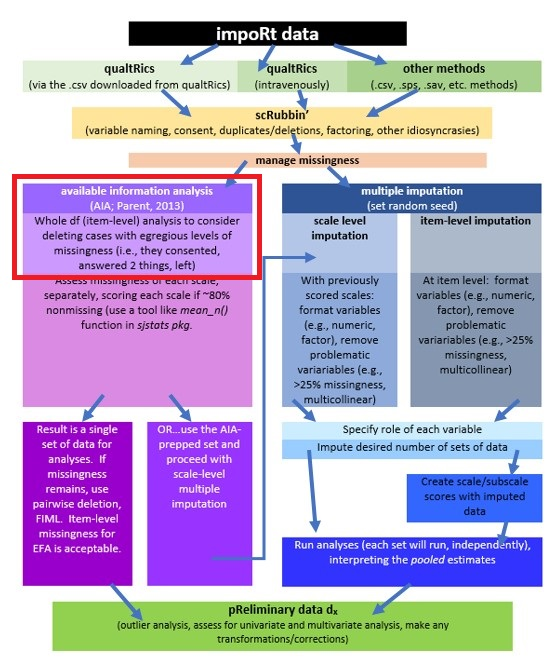
\includegraphics{images/Ch02/wrkflow_item_lvl.jpg}
\caption{An image of our stage in the workflow for scrubbing and scoring data.}
\end{figure}

Because we just created a host of new variables in creating the \emph{prop\_BIPOC} variable, let's downsize the df so that the calculations are sensible.

\begin{Shaded}
\begin{Highlighting}[]
\NormalTok{scrub\_df }\OtherTok{\textless{}{-}}\NormalTok{ (}\FunctionTok{select}\NormalTok{(scrub\_df, ID, iBIPOC\_pr, cmBlack, Belong\_1}\SpecialCharTok{:}\NormalTok{Belong\_3,}
\NormalTok{    Blst\_1}\SpecialCharTok{:}\NormalTok{Blst\_6))}
\end{Highlighting}
\end{Shaded}

With a couple of calculations, we create a proportion of item-level missingness.

In this chunk I first calculate the number of missing (nmiss)

\begin{Shaded}
\begin{Highlighting}[]
\FunctionTok{library}\NormalTok{(tidyverse)}
\CommentTok{\#Calculating number and proportion of item{-}level missingness}
\NormalTok{scrub\_df}\SpecialCharTok{$}\NormalTok{nmiss }\OtherTok{\textless{}{-}}\NormalTok{ scrub\_df}\SpecialCharTok{\%\textgreater{}\%}
    \FunctionTok{select}\NormalTok{(iBIPOC\_pr}\SpecialCharTok{:}\NormalTok{Blst\_6) }\SpecialCharTok{\%\textgreater{}\%} \CommentTok{\#the colon allows us to include all variables between the two listed (the variables need to be in order)}
\NormalTok{    is.na }\SpecialCharTok{\%\textgreater{}\%} 
\NormalTok{    rowSums}

\NormalTok{scrub\_df}\OtherTok{\textless{}{-}}\NormalTok{ scrub\_df}\SpecialCharTok{\%\textgreater{}\%}
\NormalTok{  dplyr}\SpecialCharTok{::}\FunctionTok{mutate}\NormalTok{(}\AttributeTok{prop\_miss =}\NormalTok{ (nmiss}\SpecialCharTok{/}\DecValTok{11}\NormalTok{)}\SpecialCharTok{*}\DecValTok{100}\NormalTok{) }\CommentTok{\#11 is the number of variables included in calculating the proportion}
\end{Highlighting}
\end{Shaded}

We can grab the descriptives for the \emph{prop\_miss} variable to begin to understand our data. I will create an object from it so I can use it with inline

\begin{Shaded}
\begin{Highlighting}[]
\NormalTok{psych}\SpecialCharTok{::}\FunctionTok{describe}\NormalTok{(scrub\_df}\SpecialCharTok{$}\NormalTok{prop\_miss)}
\end{Highlighting}
\end{Shaded}

\begin{verbatim}
##    vars  n mean    sd median trimmed mad min max range skew kurtosis   se
## X1    1 69 7.77 22.61      0    1.59   0   0 100   100 3.04     8.19 2.72
\end{verbatim}

CUMULATIVE CAPTURE FOR WRITING IT UP:

\begin{quote}
\begin{quote}
Across cases that were deemed eligible on the basis of the inclusion/exclusion criteria, missingness ranged from 0 to 100\%.
\end{quote}
\end{quote}

At the time that I am lecturing this, we do have some rather egregious missingness. At this point I will write code to eliminate cases with \(\geq\) 90\%.

\begin{Shaded}
\begin{Highlighting}[]
\NormalTok{scrub\_df }\OtherTok{\textless{}{-}}\NormalTok{ dplyr}\SpecialCharTok{::}\FunctionTok{filter}\NormalTok{(scrub\_df, prop\_miss }\SpecialCharTok{\textless{}=} \DecValTok{90}\NormalTok{)  }\CommentTok{\#update df to have only those with at least 90\% of complete data}
\end{Highlighting}
\end{Shaded}

To analyze missingness at this level, we need a df that has only the variables of interest. That is, variables like \emph{ID} and the \emph{prop\_miss} and \emph{nmiss} variables we created will interfere with an accurate assessment of missingness. I will update our df to eliminate these.

\begin{Shaded}
\begin{Highlighting}[]
\CommentTok{\# further update to exclude the n\_miss and prop\_miss variables}
\NormalTok{scrub\_df }\OtherTok{\textless{}{-}}\NormalTok{ scrub\_df }\SpecialCharTok{\%\textgreater{}\%}
\NormalTok{    dplyr}\SpecialCharTok{::}\FunctionTok{select}\NormalTok{(}\SpecialCharTok{{-}}\FunctionTok{c}\NormalTok{(ID, nmiss, prop\_miss))}
\end{Highlighting}
\end{Shaded}

Missing data analysis commonly looks at proportions by:

\begin{itemize}
\tightlist
\item
  the entire df
\item
  rows/cases/people
\end{itemize}

\begin{Shaded}
\begin{Highlighting}[]
\CommentTok{\# what proportion of cells missing across entire dataset}
\NormalTok{formattable}\SpecialCharTok{::}\FunctionTok{percent}\NormalTok{(}\FunctionTok{mean}\NormalTok{(}\FunctionTok{is.na}\NormalTok{(scrub\_df)))}
\end{Highlighting}
\end{Shaded}

\begin{verbatim}
## [1] 3.86%
\end{verbatim}

\begin{Shaded}
\begin{Highlighting}[]
\CommentTok{\# what proportion of cases (rows) are complete (nonmissing)}
\NormalTok{formattable}\SpecialCharTok{::}\FunctionTok{percent}\NormalTok{(}\FunctionTok{mean}\NormalTok{(}\FunctionTok{complete.cases}\NormalTok{(scrub\_df)))}
\end{Highlighting}
\end{Shaded}

\begin{verbatim}
## [1] 87.88%
\end{verbatim}

CUMULATIVE CAPTURE FOR WRITING IT UP:

\begin{quote}
\begin{quote}
Across cases that were deemed eligible on the basis of the inclusion/exclusion criteria, missingness ranged from 0 to 100\%. Across the dataset, 3.86\% of cells had missing data and 87.88\% of cases had nonmissing data.
\end{quote}
\end{quote}

\hypertarget{analyzing-missing-data-patterns}{%
\subsection{Analyzing Missing Data Patterns}\label{analyzing-missing-data-patterns}}

One approach to analyzing missing data is to assess patterns of missingness.

Several R packages are popularly used for conducting such analyses. In the \emph{mice} package, \emph{md.pattern()} function provides a matrix with the number of columns + 1, in which each row corresponds to a missing data pattern (1 = observed, 0 = missing).

Rows and columns are sorted in increasing amounts of missing information.

The last column and row contain row and column counts, respectively.

\begin{Shaded}
\begin{Highlighting}[]
\NormalTok{mice\_out }\OtherTok{\textless{}{-}}\NormalTok{ mice}\SpecialCharTok{::}\FunctionTok{md.pattern}\NormalTok{(scrub\_df, }\AttributeTok{plot =} \ConstantTok{TRUE}\NormalTok{, }\AttributeTok{rotate.names =} \ConstantTok{TRUE}\NormalTok{)}
\NormalTok{mice\_out}
\FunctionTok{write.csv}\NormalTok{(mice\_out, }\AttributeTok{file =} \StringTok{"mice\_out.csv"}\NormalTok{)  }\CommentTok{\#optional to write it to a .csv file}
\end{Highlighting}
\end{Shaded}

The table lets us examine each missing pattern and see which variable(s) is/are missing. The output is in the form of a table that indicates the frequency of each pattern of missingness. Because I haven't (yet) figured out how to pipe objects from this table into the chapter, this text may differ from the patterns in the current data frame.

Each row in the table represents a different pattern of missingness. At the time of writing, there are \emph{8} patterns of missing data. The patterns are listed in descending order of the least amount of missingness. The most common pattern (\emph{58} cases, top row) is one with no missing data. One case is missing one cell -- one item assessing the campus climate for Black students, and so forth.

\hypertarget{can-we-identify-the-missing-mechanisms}{%
\subsection{Can we identify the missing mechanisms?}\label{can-we-identify-the-missing-mechanisms}}

To date, we do not have statistical tools that can accurately diagnose our patterns of missingness. You may have heard that ``Little's MCAR'' is a helpful tool. Unfortunately, as Enders \citeyearpar{enders_applied_2010} has noted, the tool is problematic. Perhaps the most significant one is that under the null hypothesis, a statistically significant test indicates that the missing data are MAR (missing at random) or MNAR (missing not at random); a non-significant test indicates the data are MCAR (missing completely at random) or MNAR. Consequently, regardless of the result, an MNAR circumstance cannot be ruled out. Correspondingly, the Little's MCAR test has disappeared from the more reliable R packages that assess missingness.

Enders \citeyearpar{enders_applied_2010} \emph{Applied Missing Data Analysis} text does provide a set of \href{https://www.google.com/books/edition/Applied_Missing_Data_Analysis/uHt4EAAAQBAJ?hl=en\&gbpv=1\&dq=enders+missing+data\&pg=PP1\&printsec=frontcover}{figures} (page 3) that illustrate common missing data patterns. Comparing these to the figure produced with \emph{mice::mdpattern} our data looks somewhat monotonic -- that is, as individuals completed the survey, they began to experience test fatigue and simply stopped responding. Diagnosisng monotonicity requires that the variables in the dataset must be in the order in which the students completed them. If the variables have been re-ordered or if the surveys were presented to students in a randomized order, then more data manipulation would be required before attributing missingness to test fatigue.

Survey programs like Qualtrics offer the randomization of items within blocks (or blocks themselves). This can help distribute missingness caused by test fatigue so that more cases can be retained.

\hypertarget{scoring}{%
\section{Scoring}\label{scoring}}

So let's get to work to score up the measures for our analysis. Each step of this should involve careful cross-checking with the \href{https://github.com/lhbikos/ReC_MultivModel/blob/main/Rate_a_Course_Codebook.pdf}{codebook}.

\hypertarget{reverse-scoring}{%
\subsection{Reverse scoring}\label{reverse-scoring}}

As we discovered previously, in the scale that assesses campus climate (higher scores reflect a more negative climate) one of our items (Blst\_1, ``My \emph{institution} provides a supportive environment for Black students.'') requires reverse-coding.

To rescore:

\begin{itemize}
\tightlist
\item
  Create a \emph{new} variable (this is essential) that is designated as the reversed item. We might put a the letter ``r'' (for reverse scoring) at the beginning or end: rBlst\_1 or Blst\_1r. It does not matter; just be consistent.

  \begin{itemize}
  \tightlist
  \item
    We don't reverse score into the same variable because when you rerun the script, it just re-reverses the reversed score\ldots into infinity. It's very easy to lose your place.
  \end{itemize}
\item
  The reversal is an \emph{equation} where you subtract the value in the item from the range/scaling + 1. For the our three items we subtract each item's value from 8.
\end{itemize}

\begin{Shaded}
\begin{Highlighting}[]
\NormalTok{scrub\_df }\OtherTok{\textless{}{-}}\NormalTok{ scrub\_df }\SpecialCharTok{\%\textgreater{}\%}
\NormalTok{    dplyr}\SpecialCharTok{::}\FunctionTok{mutate}\NormalTok{(}\AttributeTok{rBlst\_1 =} \DecValTok{8} \SpecialCharTok{{-}}\NormalTok{ Blst\_1)  }\CommentTok{\#if you had multiple items, you could add a pipe (\%\textgreater{}\%) at the end of the line and add more until the last one}
\end{Highlighting}
\end{Shaded}

Per Parent \citeyearpar{parent_handling_2013} we will analyze missingness for each scale, separately.

\begin{itemize}
\tightlist
\item
  We will calculate scale scores on each scale separately when 80\% (roughly) of the data is present.

  \begin{itemize}
  \tightlist
  \item
    this is somewhat arbitrary, on 4 item scales, I would choose 75\% (to allow one to be missing)
  \item
    on the 3 item scale, I will allow one item to be missing (65\%)
  \end{itemize}
\item
  After calculating the scale scores, we will return to analyzing the missingness, looking at the whole df
\end{itemize}

The \emph{mean\_n()} function of \emph{sjstats} package has allows you to specify how many items (whole number) or what percentage of items should be present in order to get the mean. First, though, we should identify the variables (properly formatted, if rescoring was needed) that should be included in the calculation of each scale and subscale.

In our case, the scale assessing belonging \citep{bollen_perceived_1990, hurtado_effects_1997} involves three items with no reversals. Our campus climate scale was adapted from Szymanski et al.'s LGBTQ College Campus Climate Scale \citep{szymanski_perceptions_2020}. While it has not been psychometrically evaluated for the purpose for which I am using it, I will follow the scoring structure in the journal article that introduces the measure. Specifically, the factor structure permits a total scale score and two subscales representing the college response and stigma.

\begin{Shaded}
\begin{Highlighting}[]
\CommentTok{\# Making the list of variables}
\NormalTok{Belonging\_vars }\OtherTok{\textless{}{-}} \FunctionTok{c}\NormalTok{(}\StringTok{"Belong\_1"}\NormalTok{, }\StringTok{"Belong\_2"}\NormalTok{, }\StringTok{"Belong\_3"}\NormalTok{)}
\NormalTok{ResponseBL\_vars }\OtherTok{\textless{}{-}} \FunctionTok{c}\NormalTok{(}\StringTok{"rBlst\_1"}\NormalTok{, }\StringTok{"Blst\_4"}\NormalTok{, }\StringTok{"Blst\_6"}\NormalTok{)}
\NormalTok{StigmaBL\_vars }\OtherTok{\textless{}{-}} \FunctionTok{c}\NormalTok{(}\StringTok{"Blst\_2"}\NormalTok{, }\StringTok{"Blst\_3"}\NormalTok{, }\StringTok{"Blst\_5"}\NormalTok{)}
\NormalTok{ClimateBL\_vars }\OtherTok{\textless{}{-}} \FunctionTok{c}\NormalTok{(}\StringTok{"rBlst\_1"}\NormalTok{, }\StringTok{"Blst\_4"}\NormalTok{, }\StringTok{"Blst\_6"}\NormalTok{, }\StringTok{"Blst\_2"}\NormalTok{, }\StringTok{"Blst\_3"}\NormalTok{,}
    \StringTok{"Blst\_5"}\NormalTok{)}

\CommentTok{\# Creating the new variables}
\NormalTok{scrub\_df}\SpecialCharTok{$}\NormalTok{Belonging }\OtherTok{\textless{}{-}}\NormalTok{ sjstats}\SpecialCharTok{::}\FunctionTok{mean\_n}\NormalTok{(scrub\_df[, Belonging\_vars], }\FloatTok{0.65}\NormalTok{)}
\NormalTok{scrub\_df}\SpecialCharTok{$}\NormalTok{ResponseBL }\OtherTok{\textless{}{-}}\NormalTok{ sjstats}\SpecialCharTok{::}\FunctionTok{mean\_n}\NormalTok{(scrub\_df[, ResponseBL\_vars], }\FloatTok{0.8}\NormalTok{)}
\NormalTok{scrub\_df}\SpecialCharTok{$}\NormalTok{StigmaBL }\OtherTok{\textless{}{-}}\NormalTok{ sjstats}\SpecialCharTok{::}\FunctionTok{mean\_n}\NormalTok{(scrub\_df[, StigmaBL\_vars], }\FloatTok{0.8}\NormalTok{)}
\NormalTok{scrub\_df}\SpecialCharTok{$}\NormalTok{ClimateBL }\OtherTok{\textless{}{-}}\NormalTok{ sjstats}\SpecialCharTok{::}\FunctionTok{mean\_n}\NormalTok{(scrub\_df[, ClimateBL\_vars], }\FloatTok{0.8}\NormalTok{)}
\end{Highlighting}
\end{Shaded}

Later it will be helpful to have a df with the item and scale-level variables. It will also be helpful if there is an ID for each case.

\begin{Shaded}
\begin{Highlighting}[]
\NormalTok{scrub\_df }\OtherTok{\textless{}{-}}\NormalTok{ scrub\_df }\SpecialCharTok{\%\textgreater{}\%}
\NormalTok{    dplyr}\SpecialCharTok{::}\FunctionTok{mutate}\NormalTok{(}\AttributeTok{ID =} \FunctionTok{row\_number}\NormalTok{())}

\CommentTok{\# moving the ID number to the first column; requires}
\NormalTok{scrub\_df }\OtherTok{\textless{}{-}}\NormalTok{ scrub\_df }\SpecialCharTok{\%\textgreater{}\%}
\NormalTok{    dplyr}\SpecialCharTok{::}\FunctionTok{select}\NormalTok{(ID, }\FunctionTok{everything}\NormalTok{())}
\end{Highlighting}
\end{Shaded}

Let's save our \emph{scrub\_df} data for this and write it as an outfile. I will save it in both .rds and .csv formats so that you can use either one.

\begin{Shaded}
\begin{Highlighting}[]
\FunctionTok{write.table}\NormalTok{(scrub\_df, }\AttributeTok{file =} \StringTok{"BlStItmsScrs230902.csv"}\NormalTok{, }\AttributeTok{sep =} \StringTok{","}\NormalTok{, }\AttributeTok{col.names =} \ConstantTok{TRUE}\NormalTok{,}
    \AttributeTok{row.names =} \ConstantTok{FALSE}\NormalTok{)}
\FunctionTok{saveRDS}\NormalTok{(scrub\_df, }\StringTok{"BlStItmsScrs230902.rds"}\NormalTok{)}
\end{Highlighting}
\end{Shaded}

\hypertarget{missing-analysis-scale-level}{%
\section{Missing Analysis: Scale level}\label{missing-analysis-scale-level}}

Let's return to analyzing the missingness, this time including the \emph{scale level} variables (without the individual items) that will be in our statistical model(s).

\begin{figure}
\centering
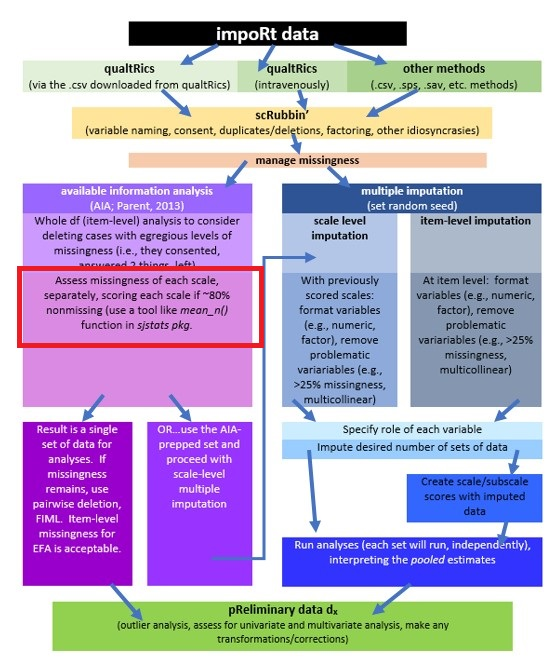
\includegraphics{images/Ch02/wrkflow_scale_lvl.jpg}
\caption{An image of our stage in the workflow for scrubbing and scoring data.}
\end{figure}

First let's get the df down to the variables we want to retain:

\begin{Shaded}
\begin{Highlighting}[]
\NormalTok{scored }\OtherTok{\textless{}{-}}\NormalTok{ dplyr}\SpecialCharTok{::}\FunctionTok{select}\NormalTok{(scrub\_df, iBIPOC\_pr, cmBlack, Belonging, ResponseBL,}
\NormalTok{    StigmaBL, ClimateBL)}
\NormalTok{ScoredCaseMiss }\OtherTok{\textless{}{-}} \FunctionTok{nrow}\NormalTok{(scored)  }\CommentTok{\#I produced this object for the sole purpose of feeding the number of cases into the inline text, below}
\NormalTok{ScoredCaseMiss}
\end{Highlighting}
\end{Shaded}

\begin{verbatim}
## [1] 66
\end{verbatim}

Before we start our formal analysis of missingness at the scale level, let's continue to scrub by eliminating cases that will have too much missingness. In the script below we create a variable that counts the number of missing variables and then creates a proportion by dividing it by the number of total variables.

Using the \emph{describe()} function from the \emph{psych} package, we can investigate this variable.

\begin{Shaded}
\begin{Highlighting}[]
\CommentTok{\# Create a variable (n\_miss) that counts the number missing}
\NormalTok{scored}\SpecialCharTok{$}\NormalTok{n\_miss }\OtherTok{\textless{}{-}}\NormalTok{ scored }\SpecialCharTok{\%\textgreater{}\%}
\NormalTok{    dplyr}\SpecialCharTok{::}\FunctionTok{select}\NormalTok{(iBIPOC\_pr}\SpecialCharTok{:}\NormalTok{ClimateBL) }\SpecialCharTok{\%\textgreater{}\%}
\NormalTok{    is.na }\SpecialCharTok{\%\textgreater{}\%}
\NormalTok{    rowSums}

\CommentTok{\# Create a proportion missing by dividing n\_miss by the total number}
\CommentTok{\# of variables (6) Pipe to sort in order of descending frequency to}
\CommentTok{\# get a sense of the missingness}
\NormalTok{scored }\OtherTok{\textless{}{-}}\NormalTok{ scored }\SpecialCharTok{\%\textgreater{}\%}
\NormalTok{    dplyr}\SpecialCharTok{::}\FunctionTok{mutate}\NormalTok{(}\AttributeTok{prop\_miss =}\NormalTok{ (n\_miss}\SpecialCharTok{/}\DecValTok{6}\NormalTok{) }\SpecialCharTok{*} \DecValTok{100}\NormalTok{) }\SpecialCharTok{\%\textgreater{}\%}
    \FunctionTok{arrange}\NormalTok{(}\FunctionTok{desc}\NormalTok{(n\_miss))}

\NormalTok{psych}\SpecialCharTok{::}\FunctionTok{describe}\NormalTok{(scored}\SpecialCharTok{$}\NormalTok{prop\_miss)}
\end{Highlighting}
\end{Shaded}

\begin{verbatim}
##    vars  n mean    sd median trimmed mad min   max range skew kurtosis   se
## X1    1 66 3.79 12.33      0    0.31   0   0 66.67 66.67 3.44    11.77 1.52
\end{verbatim}

CUMULATIVE CAPTURE FOR WRITING IT UP:

\begin{quote}
\begin{quote}
Across cases that were deemed eligible on the basis of the inclusion/exclusion criteria, missingness ranged from 0 to 100\%. Across the dataset, 3.86\% of cells had missing data and 87.88\% of cases had nonmissing data.
\end{quote}
\end{quote}

\begin{quote}
\begin{quote}
Across the 66 cases for which the scoring protocol was applied, missingness ranged from 0 to 67\%.
\end{quote}
\end{quote}

We need to decide what is our retention threshhold. Twenty percent seems to be a general rule of thumb. Let's delete all cases with missingness at 20\% or greater.

\begin{Shaded}
\begin{Highlighting}[]
\CommentTok{\# update df to have only those with at least 20\% of complete data}
\CommentTok{\# (this is an arbitrary decision)}
\NormalTok{scored }\OtherTok{\textless{}{-}}\NormalTok{ dplyr}\SpecialCharTok{::}\FunctionTok{filter}\NormalTok{(scored, prop\_miss }\SpecialCharTok{\textless{}=} \DecValTok{20}\NormalTok{)}

\CommentTok{\# the variable selection just lops off the proportion missing}
\NormalTok{scored }\OtherTok{\textless{}{-}}\NormalTok{ (}\FunctionTok{select}\NormalTok{(scored, iBIPOC\_pr}\SpecialCharTok{:}\NormalTok{ClimateBL))}

\CommentTok{\# this produces the number of cases retained}
\FunctionTok{nrow}\NormalTok{(scored)}
\end{Highlighting}
\end{Shaded}

\begin{verbatim}
## [1] 61
\end{verbatim}

CUMULATIVE CAPTURE FOR WRITING IT UP:

\begin{quote}
\begin{quote}
Across cases that were deemed eligible on the basis of the inclusion/exclusion criteria, missingness ranged from 0 to 100\%. Across the dataset, 3.86\% of cells had missing data and 87.88\% of cases had nonmissing data.
\end{quote}
\end{quote}

\begin{quote}
\begin{quote}
Across the 66 cases for which the scoring protocol was applied, missingness ranged from 0 to 67\%. After eliminating cases with greater than 20\% missing, the dataset analyzed included 61 cases.
\end{quote}
\end{quote}

With a decision about the number of cases we are going to include, we can continue to analyze missingness.

\hypertarget{revisiting-missing-analysis-at-the-scale-level}{%
\section{Revisiting Missing Analysis at the Scale Level}\label{revisiting-missing-analysis-at-the-scale-level}}

We work with a df that includes only the variables in our model. In our case this is easy. In other cases (i.e., maybe there is an ID number) it might be good to create a subset just for this analysis.

Again, we look at missingness as the proportion of

\begin{itemize}
\tightlist
\item
  individual cells across the scored dataset, and
\item
  rows/cases with nonmissing data
\end{itemize}

\begin{Shaded}
\begin{Highlighting}[]
\CommentTok{\# percent missing across df}
\NormalTok{formattable}\SpecialCharTok{::}\FunctionTok{percent}\NormalTok{(}\FunctionTok{mean}\NormalTok{(}\FunctionTok{is.na}\NormalTok{(scored)))}
\end{Highlighting}
\end{Shaded}

\begin{verbatim}
## [1] 0.55%
\end{verbatim}

\begin{Shaded}
\begin{Highlighting}[]
\CommentTok{\# percent of rows with nonmissing data}
\NormalTok{formattable}\SpecialCharTok{::}\FunctionTok{percent}\NormalTok{(}\FunctionTok{mean}\NormalTok{(}\FunctionTok{complete.cases}\NormalTok{(scored)))}
\end{Highlighting}
\end{Shaded}

\begin{verbatim}
## [1] 96.72%
\end{verbatim}

CUMULATIVE CAPTURE FOR WRITING IT UP:

\begin{quote}
\begin{quote}
Across cases that were deemed eligible on the basis of the inclusion/exclusion criteria, missingness ranged from 0 to 100\%. Across the dataset, 3.86\% of cells had missing data and 87.88\% of cases had nonmissing data.
\end{quote}
\end{quote}

\begin{quote}
\begin{quote}
Across the 66 cases for which the scoring protocol was applied, missingness ranged from 0 to 67\%. After eliminating cases with greater than 20\% missing, the dataset analyzed included 61 cases. In this dataset we had less than 1\% (0.55\%) missing across the df; 97\% of the rows had nonmissing data.
\end{quote}
\end{quote}

Let's look again at missing patterns and mechanisms.

\hypertarget{scale-level-patterns-of-missing-data}{%
\subsection{Scale Level: Patterns of Missing Data}\label{scale-level-patterns-of-missing-data}}

Returning to the \emph{mice} package, we can use the \emph{md.pattern()} function to examine a matrix with the number of columns + 1 in which each row corresponds to a missing data pattern (1 = observed, 0 = missing). The rows and columns are sorted in increasing amounts of missing information. The last column and row contain row and column counts, respectively.

\begin{Shaded}
\begin{Highlighting}[]
\NormalTok{mice\_ScaleLvl }\OtherTok{\textless{}{-}}\NormalTok{ mice}\SpecialCharTok{::}\FunctionTok{md.pattern}\NormalTok{(scored, }\AttributeTok{plot =} \ConstantTok{TRUE}\NormalTok{, }\AttributeTok{rotate.names =} \ConstantTok{TRUE}\NormalTok{)}
\end{Highlighting}
\end{Shaded}

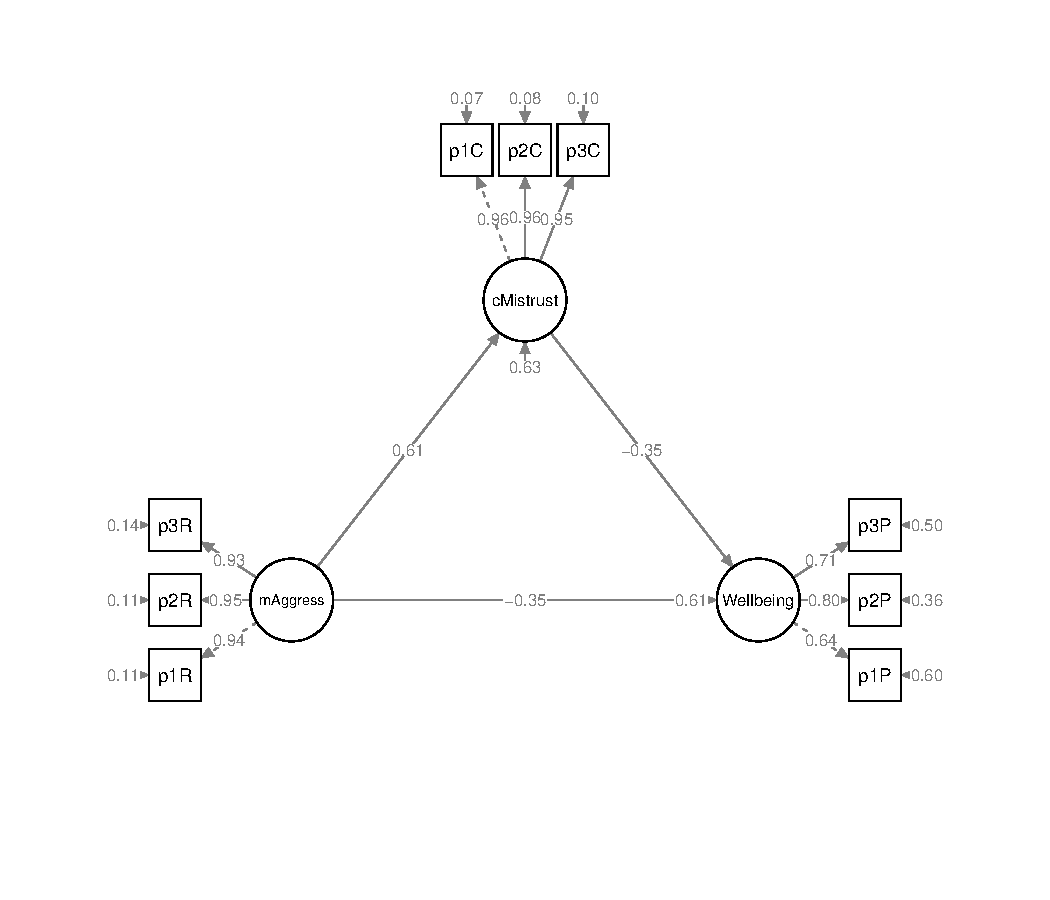
\includegraphics{02-Scoring_files/figure-latex/unnamed-chunk-26-1.pdf}

\begin{Shaded}
\begin{Highlighting}[]
\NormalTok{mice\_ScaleLvl}
\end{Highlighting}
\end{Shaded}

\begin{verbatim}
##    cmBlack Belonging ResponseBL StigmaBL ClimateBL iBIPOC_pr  
## 59       1         1          1        1         1         1 0
## 2        1         1          1        1         1         0 1
##          0         0          0        0         0         2 2
\end{verbatim}

At the scale-level, this is much easier to interpret. There are \emph{2} rows of data because there are only \emph{2} patterns of missingness. The most common pattern is non-missing data (\emph{n} = 59).

If our statistical choice uses listwise deletion (i.e., the case is eliminated if one or more variables in the model has missing data), our sample size will be 59. As we will earn in later chapters, there are alternatives (i.e., specifying a FIML option in analyses that use maximum likelihood estimators) that can use all of the cases -- even those with missing data.

\hypertarget{r-eady-for-analysis}{%
\subsection{R-eady for Analysis}\label{r-eady-for-analysis}}

At this stage the data is ready for analysis (data diagnostics). With the AIA approach \citep{parent_handling_2013} the following preliminary analyses would involve pairwise deletion (i.e., the row/case is dropped for that analysis, but included for all others):

\begin{figure}
\centering
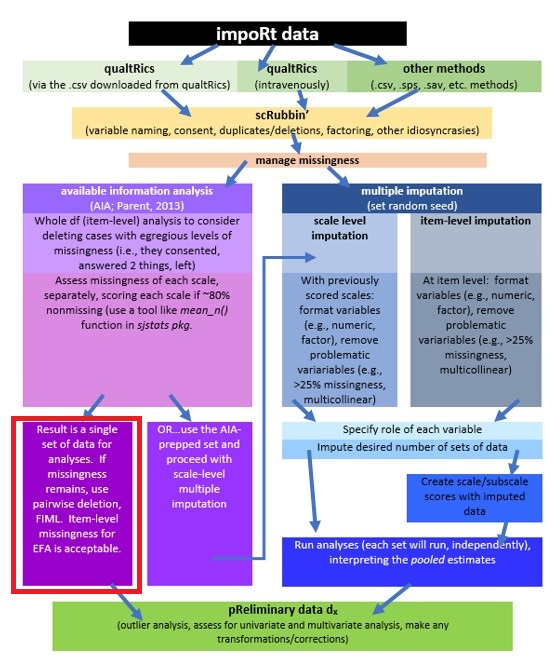
\includegraphics{images/Ch02/wrkflow_AIAready.jpg}
\caption{An image of our stage in the workflow for scrubbing and scoring data.}
\end{figure}

\begin{itemize}
\tightlist
\item
  data diagnostics

  \begin{itemize}
  \tightlist
  \item
    psychometric properties of scales, such as alpha coefficients
  \item
    assessing assumptions such as univariate and multivariate normality, outliers, etc.
  \end{itemize}
\item
  preliminary analyses

  \begin{itemize}
  \tightlist
  \item
    descriptives (means/standard deviations, frequencies)
  \item
    correlation matrices
  \end{itemize}
\end{itemize}

AIA can also be used with primary analyses. Examples of how to manage missingness include:

\begin{itemize}
\tightlist
\item
  ANOVA/regression models

  \begin{itemize}
  \tightlist
  \item
    if completed with ordinary least squares, pairwise deletion would be utilized
  \end{itemize}
\item
  SEM/CFA models with observed, latent, or hybrid models

  \begin{itemize}
  \tightlist
  \item
    if FIML (we'll discuss later) is specified, all cases are used, even when there is missingness
  \end{itemize}
\item
  EFA models

  \begin{itemize}
  \tightlist
  \item
    these can handle item-level missingness
  \end{itemize}
\item
  Hierarchical linear modeling/multilevel modeling/mixed effects modeling

  \begin{itemize}
  \tightlist
  \item
    While all data needs to be present for a given cluster/wave, it is permissible to have varying numbers of clusters/waves per case
  \end{itemize}
\end{itemize}

\hypertarget{the-apa-style-write-up}{%
\section{The APA Style Write-Up}\label{the-apa-style-write-up}}

\hypertarget{results}{%
\section{Results}\label{results}}

\begin{quote}
\begin{quote}
All analyses were completed in R Studio (v. RStudio 2023.06.1+524 ``Mountain Hydrangea'') with R (v. 4.3.1).
\end{quote}
\end{quote}

\begin{quote}
\begin{quote}
\textbf{Missing Data Analysis and Treatment of Missing Data}
\end{quote}
\end{quote}

\begin{quote}
\begin{quote}
Available item analysis (AIA; \citep{parent_handling_2013}) is a strategy for managing missing data that uses available data for analysis and excludes cases with missing data points only for analyses in which the data points would be directly involved. Parent (2013) suggested that AIA is equivalent to more complex methods (e.g., multiple imputation) across a number of variations of sample size, magnitude of associations among items, and degree of missingness. Thus, we utilized Parent's recommendations to guide our approach to managing missing data. Missing data analyses were conducted with tools in base R as well as the R packages, \emph{psych} (v. 2.3.6) and \emph{mice} (v. 3.16.0).
\end{quote}
\end{quote}

\begin{quote}
\begin{quote}
Across cases that were deemed eligible on the basis of the inclusion/exclusion criteria, missingness ranged from 0 to 67\%. Across the dataset, 3.86\% of cells had missing data and 87.88\% of cases had nonmissing data. At this stage in the analysis, we allowed all cases with less than 90\% missing to continue to the scoring stage. Guided by Parent's \citeyearpar{parent_handling_2013} AIA approach, scales with three items were scored if at least two items were non-missing; the scale with four items was scored if it at least three non-missing items; and the scale with six items was scored if it had at least five non-missing items.
\end{quote}
\end{quote}

\begin{quote}
\begin{quote}
Across the 66 cases for which the scoring protocol was applied, missingness ranged from 0 to 67\%. After eliminating cases with greater than 20\% missing, the dataset analyzed included 61 cases. In this dataset we had less than 1\% (0.55\%) missing across the data set; 97\% of the rows had nonmissing data.
\end{quote}
\end{quote}

\hypertarget{practice-problems-1}{%
\section{Practice Problems}\label{practice-problems-1}}

The three problems described below are designed to be continuations from the previous chapter (Scrubbing). You will likely encounter challenges that were not covered in this chapter. Search for and try out solutions, knowing that there are multiple paths through the analysis. The overall notion of the suggestions for practice are to (a) properly format three variables, (b) evaluate item-level missingness, (c) score any scales, (c) evaluate scale-level missingness, (d) provide an APA-style write-up, and (e) explain it to someone.

\hypertarget{problem-1-reworking-the-chapter-problem}{%
\subsection{Problem \#1: Reworking the Chapter Problem}\label{problem-1-reworking-the-chapter-problem}}

If you chose this option in the prior chapter, you imported the data from Qualtrics, applied inclusion/exclusion criteria, renamed variables, downsized the df to the variables of interest, and wrote up the preliminary results.

\hypertarget{problem-2-use-the-rate-a-recent-course-survey-choosing-different-variables-1}{%
\subsection{\texorpdfstring{Problem \#2: Use the \emph{Rate-a-Recent-Course} Survey, Choosing Different Variables}{Problem \#2: Use the Rate-a-Recent-Course Survey, Choosing Different Variables}}\label{problem-2-use-the-rate-a-recent-course-survey-choosing-different-variables-1}}

If you chose this option in the prior chapter, you chose a minimum of three variables from the \emph{Rate-a-Recent-Course} survey to include in a simple statistical model. You imported the dat from Qualtrics, applied inclusion/exclusion criteria, renamed variables, downsized the df to the variables of interest and wrote up the preliminary results.

\hypertarget{problem-3-other-data-1}{%
\subsection{Problem \#3: Other data}\label{problem-3-other-data-1}}

If you chose this option in the prior chapter, you used raw data that was available to you. You imported it into R, applied inclusion/exclusion criteria, renamed variables, downsized the df to the variables of interest, and wrote up the preliminary results.

\hypertarget{grading-rubric-1}{%
\subsection{Grading Rubric}\label{grading-rubric-1}}

\begin{longtable}[]{@{}
  >{\raggedright\arraybackslash}p{(\columnwidth - 4\tabcolsep) * \real{0.7521}}
  >{\centering\arraybackslash}p{(\columnwidth - 4\tabcolsep) * \real{0.1282}}
  >{\centering\arraybackslash}p{(\columnwidth - 4\tabcolsep) * \real{0.1197}}@{}}
\toprule\noalign{}
\begin{minipage}[b]{\linewidth}\raggedright
Assignment Component
\end{minipage} & \begin{minipage}[b]{\linewidth}\centering
Points Possible
\end{minipage} & \begin{minipage}[b]{\linewidth}\centering
Points Earned
\end{minipage} \\
\midrule\noalign{}
\endhead
\bottomrule\noalign{}
\endlastfoot
1. Proper formatting of the items(s) in your first predictor variable & 5 & \_\_\_\_\_ \\
2. Proper formatting of the items(s) in your second predictor variable & 5 & \_\_\_\_\_ \\
3. Proper formatting of the items(s) your third predictor variable & 5 & \_\_\_\_\_ \\
4. Proper formatting of your dependent variable & 5 & \_\_\_\_\_ \\
4. Evaluate and interpret item-level missingness & 5 & \_\_\_\_\_ \\
5. Score any scales/subscales & 5 & \_\_\_\_\_ \\
7. Represent your work in an APA-style write-up (added to the writeup in the previous chapter) & 5 & \_\_\_\_\_ \\
8. Explanation to grader & 5 & \_\_\_\_\_ \\
\textbf{Totals} & 45 & \_\_\_\_\_ \\
\end{longtable}

A \emph{homeworked example} for the Scrubbing, Scoring, and DataDx lessons (combined) follows the \protect\hyperlink{DataDx}{Data Dx} lesson.

\hypertarget{DataDx}{%
\chapter{Data Dx}\label{DataDx}}

\href{https://spu.hosted.panopto.com/Panopto/Pages/Viewer.aspx?pid=43dbe818-8186-498d-8e84-acf7000acb5b}{Screencasted Lecture Link}

The focus of this chapter is \emph{data diagnostics}. We are asking the question, ``Does the data have the appropriate characteristics for the analysis we want to perform?'' Some statistics are more robust than others to violations of the assumptions about the characteristics of the data. None-the-less, we must report these characteristics when we disseminate the results.

\hypertarget{navigating-this-lesson-2}{%
\section{Navigating this Lesson}\label{navigating-this-lesson-2}}

There is about 45 minutes of lecture. If you work through the materials with me it would be plan for an additional hour.

While the majority of R objects and data you will need are created within the R script that sources the chapter, there are a few that cannot be created from within the R framework. Additionally, sometimes links fail. All original materials are provided at the \href{https://github.com/lhbikos/ReC_MultivModel}{Github site} that hosts the book. More detailed guidelines for ways to access all these materials are provided in the OER's \protect\hyperlink{ReCintro}{introduction}

\hypertarget{learning-objectives-2}{%
\subsection{Learning Objectives}\label{learning-objectives-2}}

Learning objectives from this lecture include the following:

\begin{itemize}
\tightlist
\item
  Conduct and interpret critical data diagnostics, including

  \begin{itemize}
  \tightlist
  \item
    alpha coefficients
  \item
    skew
  \item
    kurtosis
  \end{itemize}
\item
  Assess univariate and multivariate normality
\item
  Identify options for managing outliers and skewed data
\item
  Articulate a workflow for data preparation, including scrubbing, scoring, and data diagnostics
\end{itemize}

\hypertarget{planning-for-practice-2}{%
\subsection{Planning for Practice}\label{planning-for-practice-2}}

The suggestions from practice are a continuation from the two prior chapters. If you have completed one or more of those assignments, you should have started with a raw dataset and then scrubbed and scored it. This chapter will involve running basic data diagnostics. Options of graded complexity could incude:

\begin{itemize}
\tightlist
\item
  Repeating the steps in the chapter with the most recent data from the Rate-A-Recent-Course survey; differences will be in the number of people who have completed the survey since the chapter was written.
\item
  Use the dataset that is the source of the chapter, but score a different set of items that you choose.
\item
  Begin with raw data to which you have access.
\end{itemize}

\hypertarget{readings-resources-2}{%
\subsection{Readings \& Resources}\label{readings-resources-2}}

In preparing this chapter, I drew heavily from the following resource(s). Other resources are cited (when possible, linked) in the text with complete citations in the reference list.

\begin{itemize}
\tightlist
\item
  Parent, M. C. (2013). Handling item-level missing data: Simpler is just as good. The Counseling Psychologist, 41(4), 568--600. \url{https://doi.org/10.1177/0011000012445176}

  \begin{itemize}
  \tightlist
  \item
    The purpose of Parent's article was to argue that complex and resource-intensive procedurs like multiple imputation are unnecessary. Following a simulation that supports his claims, Parent provides some guidelines to follow for the AIA approach.
  \end{itemize}
\item
  Kline, R. B. (2015). Data preparation and psychometrics review. In Principles and Practice of Structural Equation Modeling, Fourth Edition. Guilford Publications. \url{http://ebookcentral.proquest.com/lib/spu/detail.action?docID=4000663}

  \begin{itemize}
  \tightlist
  \item
    Kline's chapter is my ``go-to'' for making decisions about preparing data for analysis.
  \end{itemize}
\end{itemize}

\hypertarget{packages-2}{%
\subsection{Packages}\label{packages-2}}

The packages used in this lesson are embedded in this code. When the hashtags are removed, the script below will (a) check to see if the following packages are installed on your computer and, if not (b) install them.

\begin{Shaded}
\begin{Highlighting}[]
\CommentTok{\# if(!require(tidyverse))\{install.packages(\textquotesingle{}tidyverse\textquotesingle{})\} \#this}
\CommentTok{\# includes dplyr if(!require(psych))\{install.packages(\textquotesingle{}psych\textquotesingle{})\}}
\CommentTok{\# if(!require(apaTables))\{install.packages(\textquotesingle{}apaTables\textquotesingle{})\}}
\end{Highlighting}
\end{Shaded}

\hypertarget{workflow-for-preliminary-data-diagnostics}{%
\section{Workflow for Preliminary Data Diagnostics}\label{workflow-for-preliminary-data-diagnostics}}

The same workflow guides us through the Scrubbing, Scoring, and Data Dx chapters. At this stage we have

\begin{itemize}
\tightlist
\item
  imported our raw data from Qualtrics,
\item
  scrubbed the data by applying our inclusion and exclusion criteria, and
\item
  used Parent's available information approach {[}AIA; -\citet{parent_handling_2013}{]} for determining the acceptable amount of missingness for each scale, and
\item
  prepared variables and scored them.
\end{itemize}

We are now ready to engage in data diagnostics for the statistical model we will test.

\begin{figure}
\centering
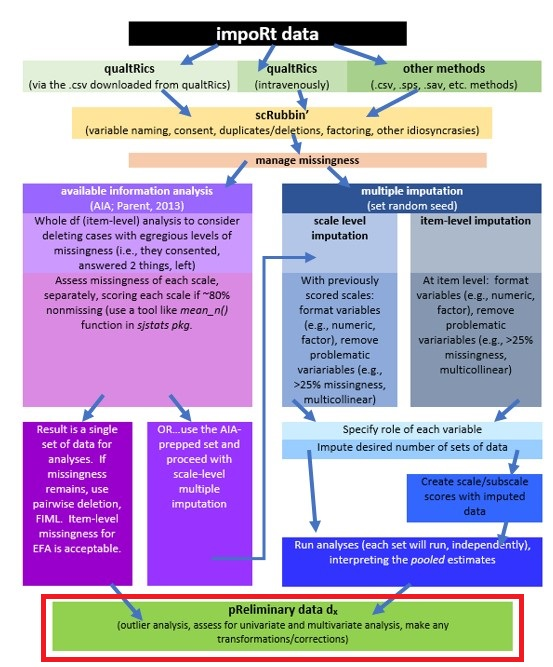
\includegraphics{images/Ch04/wrkflow_dx.jpg}
\caption{An image of our stage in the workflow for scrubbing and scoring data.}
\end{figure}

\hypertarget{research-vignette-2}{%
\section{Research Vignette}\label{research-vignette-2}}

The research vignette comes from the survey titled, \href{https://spupsych.az1.qualtrics.com/jfe/form/SV_b2cClqAlLGQ6nLU}{Rate-a-Recent-Course: A ReCentering Psych Stats Exercise} and is explained in the \protect\hyperlink{scrub}{scrubbing chapter}. In the \protect\hyperlink{score}{scoring chapter} we prepared four variables for analysis. Details for these are in our \href{./Rate-a-Course_Codebook.pdf}{codebook}.

Variable recap:

\begin{itemize}
\tightlist
\item
  Perceived Campus Climate for Black Students includes 6 items, one of which was reverse scored. This scale was adapted from Szymanski et al.'s \citeyearpar{szymanski_perceptions_2020} Campus Climate for LGBTQ students. It has not been evaluated for use with other groups. The Szymanski et al.~analysis suggested that it could be used as a total scale score, or divided into three items each that assess

  \begin{itemize}
  \tightlist
  \item
    College response to LGBTQ students (items 6, 4, 1)
  \item
    LGBTQ stigma (items 3, 2, 5)
  \end{itemize}
\item
  Sense of Belonging includes 3 items. This is a subscale from Bollen and Hoyle's \citeyearpar{bollen_perceived_1990} Perceived Cohesion Scale. There are no items on this scale that require reversing.
\item
  Percent of Black classmates is a single item that asked respondents to estimate the proportion of students in various racial categories
\item
  Percent of BIPOC instructional staff, similarly, asked respondents to identify the racial category of each member of their instructional staff
\end{itemize}

As we noted in the \protect\hyperlink{scrub}{scrubbing chapter}, our design has notable limitations. Briefly, (a) owing to the open source aspect of the data we do not ask about the demographic characteristics of the respondent; (b) the items that ask respondents to \emph{guess} the identities of the instructional staff and to place them in broad categories, (c) we do not provide a ``write-in'' a response. We made these decisions after extensive conversation with stakeholders. The primary reason for these decisions was to prevent potential harm (a) to respondents who could be identified if/when the revealed private information in this open-source survey, and (b) trolls who would write inappropriate or harmful comments.

As I think about ``how these variables go together'' (which is often where I start in planning a study), imagine a parallel mediation. That is the perception of campus climate for Black students would be predicted by the respondent's sense of belonging, mediated in separate paths through the proportion of classmates who are Black and the proportion of BIPOC instructional staff.

\emph{I would like to assess the model by having the instructional staff variable to be the \%Black instructional staff. At the time that this lecture is being prepared, there is not sufficient Black representation in the staff to model this.}

\begin{figure}
\centering
\includegraphics{images/Ch04/BlStuMed.jpg}
\caption{An image of the statistical model for which we are preparing data.}
\end{figure}

I will finish up this chapter by conducting a regression. Because parallel mediation can be complicated (I teach it in a later chapter), I will demonstrate use of our prepared variables with a simple multiple regression.

\begin{figure}
\centering
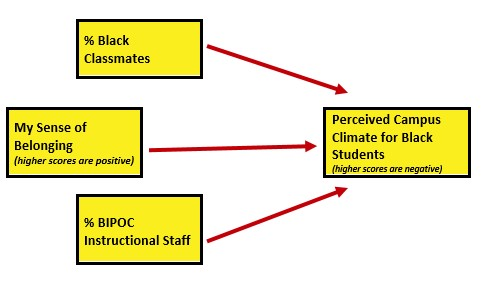
\includegraphics{images/Ch04/BlStuRegression.jpg}
\caption{An image of the statistical model for which we are preparing data.}
\end{figure}

First, though, let's take a more conceptual look at issues regarding missing data. We'll come back to details of the survey as we work with it.

\hypertarget{internal-consistency-of-scalessubscales}{%
\section{Internal Consistency of Scales/Subscales}\label{internal-consistency-of-scalessubscales}}

Alpha coefficients are \emph{reliability coefficients} that assess the \emph{internal consistency} of an instrument. It asks, ``For each person, are responses \emph{consistently} high, or medium, or low?'' To the degree that they are (meaning there are high inter-item correlations), the internal consistency coefficient will be high. We want values \textgreater.80. There are numerous problems with alpha coefficients. The biggest one is that they are influenced by sample size -- longer scales have higher alpha coefficients \citep{cortina_what_1993}. Fourteen seems to be a magic number where we begin to not trust the high alpha coefficient. I address this more thoroughly -- offering an alternative -- in psychometrics. While there is much criticism about the usefulness of the alpha coefficient \citep{sijtsma_use_2009}, researchers continue to use the alpha coefficient as an indicator of the internal consistency of scales that consist of multiple items and contain several variables.

We need item level data to compute an alpha coefficient. The easiest way to get an alpha coefficient is to feed the \emph{alpha()} function (\emph{psych} package) a concatonated list of items (with any items already reverse-scored). There should be no extra items. In the \protect\hyperlink{score}{scoring chapter} we already reverse-coded the single item in the campus climate scale, so we are ready to calculate alphas.

The df from which I am pulling data was created and written as an outfile in the \protect\hyperlink{score}{scoring chapter}. You may also download the file from the \href{https://github.com/lhbikos/ReC_MultivModel}{Github site} that hosts the chapter. Be sure to place the file in the same folder as the .rmd file. This particular df has item-level data. I am working with the .rds file. In case this is problematic for you, I have also provided code to import a .csv version of the file.

\begin{Shaded}
\begin{Highlighting}[]
\NormalTok{item\_scores\_df }\OtherTok{\textless{}{-}} \FunctionTok{readRDS}\NormalTok{(}\StringTok{"BlStItmsScrs230902.rds"}\NormalTok{)}
\CommentTok{\# item\_scores\_df \textless{}{-} read.csv(\textquotesingle{}BlStItmsScrs230902.csv\textquotesingle{}, header = TRUE)}
\end{Highlighting}
\end{Shaded}

Within the \emph{psych::alpha} function we can retrieve alpha coefficients for the specific variables of interest by imbedding a concatonated list. A priori, we are planning to use the campus climate scale as a total score. However, we'll go ahead and also calculate alpha coefficients for the subscales because (a) it's good practice and (b) if the alpha is low, a \emph{reason} might show up in one of the subscales.

\begin{Shaded}
\begin{Highlighting}[]
\CommentTok{\# alpha for the belonging scale}
\NormalTok{psych}\SpecialCharTok{::}\FunctionTok{alpha}\NormalTok{(item\_scores\_df[}\FunctionTok{c}\NormalTok{(}\StringTok{"Belong\_1"}\NormalTok{, }\StringTok{"Belong\_2"}\NormalTok{, }\StringTok{"Belong\_3"}\NormalTok{)])}
\end{Highlighting}
\end{Shaded}

\begin{verbatim}

Reliability analysis   
Call: psych::alpha(x = item_scores_df[c("Belong_1", "Belong_2", "Belong_3")])

  raw_alpha std.alpha G6(smc) average_r S/N    ase mean  sd median_r
      0.95      0.95    0.93      0.87  21 0.0099    4 1.5     0.88

    95% confidence boundaries 
         lower alpha upper
Feldt     0.93  0.95  0.97
Duhachek  0.93  0.95  0.97

 Reliability if an item is dropped:
         raw_alpha std.alpha G6(smc) average_r S/N alpha se var.r med.r
Belong_1      0.94      0.94    0.88      0.88  15    0.016    NA  0.88
Belong_2      0.92      0.92    0.85      0.85  11    0.020    NA  0.85
Belong_3      0.94      0.94    0.89      0.89  16    0.015    NA  0.89

 Item statistics 
          n raw.r std.r r.cor r.drop mean  sd
Belong_1 64  0.95  0.95  0.92   0.90  4.1 1.5
Belong_2 65  0.96  0.96  0.94   0.92  4.1 1.6
Belong_3 64  0.95  0.95  0.91   0.89  3.8 1.5

Non missing response frequency for each item
            1    2    3    4    5    6    7 miss
Belong_1 0.02 0.14 0.23 0.17 0.22 0.17 0.05 0.03
Belong_2 0.03 0.14 0.22 0.22 0.15 0.20 0.05 0.02
Belong_3 0.05 0.19 0.19 0.23 0.20 0.09 0.05 0.03
\end{verbatim}

For each scale I will capture a statement for the APA style write-up. Because these values are typically reported with each measure (and not in the prliminary results), I won't create a cumulative write-up.

\begin{quote}
\begin{quote}
Cronbach's alpha for the belonging scale was 0.95.
\end{quote}
\end{quote}

\begin{Shaded}
\begin{Highlighting}[]
\CommentTok{\# alpha for the campus climate for Black students scale}
\NormalTok{psych}\SpecialCharTok{::}\FunctionTok{alpha}\NormalTok{(item\_scores\_df[}\FunctionTok{c}\NormalTok{(}\StringTok{"rBlst\_1"}\NormalTok{, }\StringTok{"Blst\_2"}\NormalTok{, }\StringTok{"Blst\_3"}\NormalTok{, }\StringTok{"Blst\_4"}\NormalTok{,}
    \StringTok{"Blst\_5"}\NormalTok{, }\StringTok{"Blst\_6"}\NormalTok{)])}
\end{Highlighting}
\end{Shaded}

\begin{verbatim}

Reliability analysis   
Call: psych::alpha(x = item_scores_df[c("rBlst_1", "Blst_2", "Blst_3", 
    "Blst_4", "Blst_5", "Blst_6")])

  raw_alpha std.alpha G6(smc) average_r S/N  ase mean  sd median_r
      0.85      0.87    0.87      0.52 6.5 0.03  2.5 1.1     0.52

    95% confidence boundaries 
         lower alpha upper
Feldt     0.78  0.85  0.90
Duhachek  0.79  0.85  0.91

 Reliability if an item is dropped:
        raw_alpha std.alpha G6(smc) average_r S/N alpha se var.r med.r
rBlst_1      0.85      0.87    0.87      0.57 6.5    0.031 0.029  0.57
Blst_2       0.87      0.88    0.87      0.59 7.1    0.026 0.019  0.56
Blst_3       0.83      0.85    0.85      0.54 5.8    0.034 0.029  0.50
Blst_4       0.80      0.82    0.82      0.48 4.6    0.041 0.027  0.48
Blst_5       0.79      0.81    0.81      0.46 4.3    0.042 0.024  0.47
Blst_6       0.80      0.82    0.81      0.48 4.6    0.040 0.021  0.50

 Item statistics 
         n raw.r std.r r.cor r.drop mean  sd
rBlst_1 60  0.69  0.67  0.56   0.52  3.4 1.6
Blst_2  64  0.68  0.62  0.51   0.46  3.0 1.8
Blst_3  63  0.71  0.74  0.66   0.59  2.0 1.2
Blst_4  62  0.85  0.86  0.84   0.77  2.5 1.3
Blst_5  63  0.89  0.89  0.89   0.82  2.0 1.2
Blst_6  63  0.83  0.86  0.86   0.77  2.1 1.3

Non missing response frequency for each item
           1    2    3    4    5    6    7 miss
rBlst_1 0.10 0.23 0.20 0.25 0.08 0.10 0.03 0.09
Blst_2  0.33 0.16 0.09 0.17 0.16 0.06 0.03 0.03
Blst_3  0.44 0.33 0.06 0.11 0.03 0.02 0.00 0.05
Blst_4  0.27 0.34 0.15 0.18 0.05 0.00 0.02 0.06
Blst_5  0.46 0.30 0.05 0.14 0.05 0.00 0.00 0.05
Blst_6  0.38 0.35 0.11 0.08 0.06 0.02 0.00 0.05
\end{verbatim}

\begin{quote}
\begin{quote}
Cronbach's alpha for the campus climate scale was 0.87.
\end{quote}
\end{quote}

Since this value is \(\geq\) .80, it is within the realm of acceptability. Let's go ahead, though, and examine its subscales.

\begin{Shaded}
\begin{Highlighting}[]
\CommentTok{\# alpha for the stigma scale of the campus climate for Black students}
\CommentTok{\# scale}
\NormalTok{psych}\SpecialCharTok{::}\FunctionTok{alpha}\NormalTok{(item\_scores\_df[}\FunctionTok{c}\NormalTok{(}\StringTok{"Blst\_3"}\NormalTok{, }\StringTok{"Blst\_2"}\NormalTok{, }\StringTok{"Blst\_5"}\NormalTok{)])}
\end{Highlighting}
\end{Shaded}

\begin{verbatim}

Reliability analysis   
Call: psych::alpha(x = item_scores_df[c("Blst_3", "Blst_2", "Blst_5")])

  raw_alpha std.alpha G6(smc) average_r S/N   ase mean  sd median_r
      0.69      0.73    0.69      0.47 2.7 0.065  2.3 1.2     0.54

    95% confidence boundaries 
         lower alpha upper
Feldt     0.54  0.69  0.80
Duhachek  0.57  0.69  0.82

 Reliability if an item is dropped:
       raw_alpha std.alpha G6(smc) average_r  S/N alpha se var.r med.r
Blst_3      0.67      0.70    0.54      0.54 2.35    0.074    NA  0.54
Blst_2      0.75      0.75    0.60      0.60 3.03    0.061    NA  0.60
Blst_5      0.41      0.43    0.28      0.28 0.76    0.135    NA  0.28

 Item statistics 
        n raw.r std.r r.cor r.drop mean  sd
Blst_3 63  0.72  0.78  0.62   0.46    2 1.2
Blst_2 64  0.82  0.75  0.55   0.46    3 1.8
Blst_5 63  0.87  0.89  0.83   0.70    2 1.2

Non missing response frequency for each item
          1    2    3    4    5    6    7 miss
Blst_3 0.44 0.33 0.06 0.11 0.03 0.02 0.00 0.05
Blst_2 0.33 0.16 0.09 0.17 0.16 0.06 0.03 0.03
Blst_5 0.46 0.30 0.05 0.14 0.05 0.00 0.00 0.05
\end{verbatim}

\begin{quote}
\begin{quote}
Cronbach's alpha for the campus climate stigma subscale was 0.73.
\end{quote}
\end{quote}

\begin{Shaded}
\begin{Highlighting}[]
\CommentTok{\# alpha for the campus responsiveness scale of the campus climate for}
\CommentTok{\# Black students scale}
\NormalTok{psych}\SpecialCharTok{::}\FunctionTok{alpha}\NormalTok{(item\_scores\_df[}\FunctionTok{c}\NormalTok{(}\StringTok{"rBlst\_1"}\NormalTok{, }\StringTok{"Blst\_4"}\NormalTok{, }\StringTok{"Blst\_6"}\NormalTok{)])}
\end{Highlighting}
\end{Shaded}

\begin{verbatim}

Reliability analysis   
Call: psych::alpha(x = item_scores_df[c("rBlst_1", "Blst_4", "Blst_6")])

  raw_alpha std.alpha G6(smc) average_r S/N   ase mean  sd median_r
      0.79      0.81    0.76      0.58 4.2 0.045  2.7 1.2     0.52

    95% confidence boundaries 
         lower alpha upper
Feldt     0.69  0.79  0.87
Duhachek  0.71  0.79  0.88

 Reliability if an item is dropped:
        raw_alpha std.alpha G6(smc) average_r S/N alpha se var.r med.r
rBlst_1      0.86      0.86    0.75      0.75 6.0    0.035    NA  0.75
Blst_4       0.64      0.65    0.48      0.48 1.8    0.087    NA  0.48
Blst_6       0.68      0.68    0.52      0.52 2.1    0.078    NA  0.52

 Item statistics 
         n raw.r std.r r.cor r.drop mean  sd
rBlst_1 60  0.81  0.78  0.58   0.53  3.4 1.6
Blst_4  62  0.88  0.89  0.84   0.72  2.5 1.3
Blst_6  63  0.85  0.87  0.81   0.69  2.1 1.3

Non missing response frequency for each item
           1    2    3    4    5    6    7 miss
rBlst_1 0.10 0.23 0.20 0.25 0.08 0.10 0.03 0.09
Blst_4  0.27 0.34 0.15 0.18 0.05 0.00 0.02 0.06
Blst_6  0.38 0.35 0.11 0.08 0.06 0.02 0.00 0.05
\end{verbatim}

\begin{quote}
\begin{quote}
Cronbach's alpha for the campus climate responsiveness subscale was 0.80. Between the two subscales, it looks as if the responsivenes subscale is more internally consistent.
\end{quote}
\end{quote}

\hypertarget{distributional-characteristics-of-the-variables}{%
\section{Distributional Characteristics of the Variables}\label{distributional-characteristics-of-the-variables}}

\hypertarget{evaluating-univariate-normality}{%
\subsection{Evaluating Univariate Normality}\label{evaluating-univariate-normality}}

Statistics like ANOVA and regression each have a set of assumptions about the distributional characteristics of the data. In most of the chapters in this OER we review those assumptions and how to evaluate them. Common across many statistics is the requirement of univariate and multivariate normality. Let's take a look at the variables we will use in our analysis and assess those.

We can continue to work from the df we uploaded at the beginning of the chapter to do this work. Let's take a quick peek. This df has the item-level data (we used it for the alpha coefficients); the scale and subscale scores; and the two items that assess proportion of instructional staff that are BIPOC and proportion of classmates that are BIPOC.

The \emph{str()} function let's us look at the variable format/measurement level of each variable.

\begin{Shaded}
\begin{Highlighting}[]
\FunctionTok{str}\NormalTok{(item\_scores\_df)}
\end{Highlighting}
\end{Shaded}

\begin{verbatim}
Classes 'tbl_df', 'tbl' and 'data.frame':   66 obs. of  17 variables:
 $ ID        : int  1 2 3 4 5 6 7 8 9 10 ...
 $ iBIPOC_pr : num  0.333 0 0.5 0.333 1 ...
 $ cmBlack   : num  0 5 10 6 5 20 0 0 0 4 ...
  ..- attr(*, "label")= Named chr "Regarding race, what proportion of students were from each broad classification.  Your responses should add to 100%. - Black"
  .. ..- attr(*, "names")= chr "Race_1"
 $ Belong_1  : num  6 4 NA 5 4 5 6 7 6 3 ...
  ..- attr(*, "label")= Named chr "Please indicate the degree to which you agree with the following questions about the course. Please skip the it"| __truncated__
  .. ..- attr(*, "names")= chr "Belong_1"
 $ Belong_2  : num  6 4 3 3 4 6 6 7 6 3 ...
  ..- attr(*, "label")= Named chr "Please indicate the degree to which you agree with the following questions about the course. Please skip the it"| __truncated__
  .. ..- attr(*, "names")= chr "Belong_2"
 $ Belong_3  : num  7 6 NA 2 4 5 5 7 6 3 ...
  ..- attr(*, "label")= Named chr "Please indicate the degree to which you agree with the following questions about the course. Please skip the it"| __truncated__
  .. ..- attr(*, "names")= chr "Belong_3"
 $ Blst_1    : num  5 6 NA 2 6 5 5 5 5 3 ...
  ..- attr(*, "label")= Named chr "Each item below asks you to rate elements of campus climate for your \"academic department/program.\"  If you d"| __truncated__
  .. ..- attr(*, "names")= chr "Blst_1"
 $ Blst_2    : num  3 6 5 2 1 1 4 4 3 5 ...
  ..- attr(*, "label")= Named chr "Each item below asks you to rate elements of campus climate for your \"academic department/program.\"  If you d"| __truncated__
  .. ..- attr(*, "names")= chr "Blst_2"
 $ Blst_3    : num  5 2 2 2 1 1 4 3 1 2 ...
  ..- attr(*, "label")= Named chr "Each item below asks you to rate elements of campus climate for your \"academic department/program.\"  If you d"| __truncated__
  .. ..- attr(*, "names")= chr "Blst_3"
 $ Blst_4    : num  2 2 2 2 1 2 4 3 2 3 ...
  ..- attr(*, "label")= Named chr "Each item below asks you to rate elements of campus climate for your \"academic department/program.\"  If you d"| __truncated__
  .. ..- attr(*, "names")= chr "Blst_4"
 $ Blst_5    : num  2 4 NA 2 1 1 4 4 1 3 ...
  ..- attr(*, "label")= Named chr "Each item below asks you to rate elements of campus climate for your \"academic department/program.\"  If you d"| __truncated__
  .. ..- attr(*, "names")= chr "Blst_5"
 $ Blst_6    : num  2 1 2 2 1 2 4 3 2 3 ...
  ..- attr(*, "label")= Named chr "Each item below asks you to rate elements of campus climate for your \"academic department/program.\"  If you d"| __truncated__
  .. ..- attr(*, "names")= chr "Blst_6"
 $ rBlst_1   : num  3 2 NA 6 2 3 3 3 3 5 ...
  ..- attr(*, "label")= Named chr "Each item below asks you to rate elements of campus climate for your \"academic department/program.\"  If you d"| __truncated__
  .. ..- attr(*, "names")= chr "Blst_1"
 $ Belonging : num  6.33 4.67 NA 3.33 4 5.33 5.67 7 6 3 ...
 $ ResponseBL: num  2.33 1.67 2 3.33 1.33 2.33 3.67 3 2.33 3.67 ...
 $ StigmaBL  : num  3.33 4 3.5 2 1 1 4 3.67 1.67 3.33 ...
 $ ClimateBL : num  2.83 2.83 NA 2.67 1.17 1.67 3.83 3.33 2 3.5 ...
 - attr(*, "column_map")=Classes 'tbl_df', 'tbl' and 'data.frame':  182 obs. of  7 variables:
  ..$ qname      : chr [1:182] "StartDate" "EndDate" "Status" "Progress" ...
  ..$ description: chr [1:182] "Start Date" "End Date" "Response Type" "Progress" ...
  ..$ main       : chr [1:182] "Start Date" "End Date" "Response Type" "Progress" ...
  ..$ sub        : chr [1:182] "" "" "" "" ...
  ..$ ImportId   : chr [1:182] "startDate" "endDate" "status" "progress" ...
  ..$ timeZone   : chr [1:182] "America/Los_Angeles" "America/Los_Angeles" NA NA ...
  ..$ choiceId   : chr [1:182] NA NA NA NA ...
\end{verbatim}

The difference between ``int'' (integer) and ``num'' (numerical) is that integers are limited to whole numbers. For the statistics used in this lesson, both are acceptable formats for the variables.

\begin{Shaded}
\begin{Highlighting}[]
\CommentTok{\# the script may look a little complicated; I could have simply}
\CommentTok{\# written: describe(item\_scores\_df) because I only wanted only a few}
\CommentTok{\# variables, I provided them in a concatenated: list [c(\textquotesingle{}iBIPOC\_pr\textquotesingle{},}
\CommentTok{\# \textquotesingle{}cmBlack\textquotesingle{}, \textquotesingle{}Belonging\textquotesingle{}, \textquotesingle{}ClimateBL\textquotesingle{})] I used type =1 so that we can}
\CommentTok{\# interpret skew and kurtosis along Kline\textquotesingle{}s recommendations I created}
\CommentTok{\# an object from the descriptive results, this can be used to export}
\CommentTok{\# the results for easier table making or manipulation outside of R}

\NormalTok{descriptives }\OtherTok{\textless{}{-}}\NormalTok{ psych}\SpecialCharTok{::}\FunctionTok{describe}\NormalTok{(item\_scores\_df[}\FunctionTok{c}\NormalTok{(}\StringTok{"iBIPOC\_pr"}\NormalTok{, }\StringTok{"cmBlack"}\NormalTok{,}
    \StringTok{"Belonging"}\NormalTok{, }\StringTok{"ClimateBL"}\NormalTok{)], }\AttributeTok{type =} \DecValTok{1}\NormalTok{)}
\CommentTok{\# When we capture results in an object, we need to write it below so}
\CommentTok{\# the results will display}
\NormalTok{descriptives}
\end{Highlighting}
\end{Shaded}

\begin{verbatim}
          vars  n mean   sd median trimmed  mad min   max range skew kurtosis
iBIPOC_pr    1 64 0.35 0.39   0.25    0.32 0.37   0  1.00  1.00 0.64    -1.05
cmBlack      2 66 8.20 8.02   5.50    7.24 8.15   0 30.00 30.00 0.95     0.05
Belonging    3 64 4.03 1.47   4.00    4.03 1.48   1  7.00  6.00 0.03    -0.76
ClimateBL    4 61 2.48 1.09   2.33    2.41 0.99   1  5.67  4.67 0.56     0.04
            se
iBIPOC_pr 0.05
cmBlack   0.99
Belonging 0.18
ClimateBL 0.14
\end{verbatim}

\begin{Shaded}
\begin{Highlighting}[]
\CommentTok{\# this can be useful if you wish to manually format the data for an}
\CommentTok{\# APA style table}
\FunctionTok{write.csv}\NormalTok{(descriptives, }\AttributeTok{file =} \StringTok{"DataDx\_descripts.csv"}\NormalTok{)}
\end{Highlighting}
\end{Shaded}

Skew and kurtosis are one way to evaluate whether or not data are normally distributed. When we use the ``type=1'' argument, the skew and kurtosis indices in the \emph{psych} package can be interpreted according to Kline's \citeyearpar{kline_data_2016} guidelines. Regarding skew, values greater than the absolute value of 3.0 are generally considered ``severely skewed.'' Regarding kurtosis, ``severely kurtotic'' is argued to be anywhere greater 8 to 20. Kline recommended using a conservative threshold of the absolute value of 10. The skew and kurtosis values for our variables fall well below these thesholds.

We can also apply the Shapiro-Wilk test of normality to each of our variables. When the \(p\) value is \textless{} .05, the variable's distribution is deviates from a normal distribution to a degree that is statistically significant. Below, the plotting of the histogram with a normal curve superimposed shows how the distribution approximates one that is normal.

\begin{Shaded}
\begin{Highlighting}[]
\CommentTok{\# The shapiro{-}test is in base R; it\textquotesingle{}s specification is simple:}
\CommentTok{\# shapiro.test(df$variable) I added the object (and had to list it}
\CommentTok{\# below) so I can use the inline text function}
\FunctionTok{shapiro.test}\NormalTok{(item\_scores\_df}\SpecialCharTok{$}\NormalTok{cmBlack)}
\end{Highlighting}
\end{Shaded}

\begin{verbatim}

    Shapiro-Wilk normality test

data:  item_scores_df$cmBlack
W = 0.87796, p-value = 0.000009899
\end{verbatim}

\begin{Shaded}
\begin{Highlighting}[]
\FunctionTok{shapiro.test}\NormalTok{(item\_scores\_df}\SpecialCharTok{$}\NormalTok{iBIPOC\_pr)}
\end{Highlighting}
\end{Shaded}

\begin{verbatim}

    Shapiro-Wilk normality test

data:  item_scores_df$iBIPOC_pr
W = 0.78725, p-value = 0.00000003181
\end{verbatim}

\begin{Shaded}
\begin{Highlighting}[]
\FunctionTok{shapiro.test}\NormalTok{(item\_scores\_df}\SpecialCharTok{$}\NormalTok{Belonging)}
\end{Highlighting}
\end{Shaded}

\begin{verbatim}

    Shapiro-Wilk normality test

data:  item_scores_df$Belonging
W = 0.97262, p-value = 0.1654
\end{verbatim}

\begin{Shaded}
\begin{Highlighting}[]
\FunctionTok{shapiro.test}\NormalTok{(item\_scores\_df}\SpecialCharTok{$}\NormalTok{ClimateBL)}
\end{Highlighting}
\end{Shaded}

\begin{verbatim}

    Shapiro-Wilk normality test

data:  item_scores_df$ClimateBL
W = 0.95102, p-value = 0.01613
\end{verbatim}

\hypertarget{pairs-panels}{%
\subsection{Pairs Panels}\label{pairs-panels}}

As we work our way from univariate to multivariate inspection of our data, let's take a look at the bivariate relations.

The \emph{pairs.panels()} function from the \emph{psych} package is useful for showing the relationship between variables (probably no more than 10) in a model.

\begin{itemize}
\tightlist
\item
  The lower half is a scatterplot between the two variables with a regression line (red) and mean (dot).\\
\item
  The diagonal is a histogram of each variable.\\
\item
  The upper half of is the correlation coefficient between the two variables.
\end{itemize}

\begin{Shaded}
\begin{Highlighting}[]
\NormalTok{psych}\SpecialCharTok{::}\FunctionTok{pairs.panels}\NormalTok{(item\_scores\_df[}\FunctionTok{c}\NormalTok{(}\StringTok{"iBIPOC\_pr"}\NormalTok{, }\StringTok{"cmBlack"}\NormalTok{, }\StringTok{"Belonging"}\NormalTok{,}
    \StringTok{"ClimateBL"}\NormalTok{)], }\AttributeTok{stars =} \ConstantTok{TRUE}\NormalTok{, }\AttributeTok{lm =} \ConstantTok{TRUE}\NormalTok{)}
\end{Highlighting}
\end{Shaded}

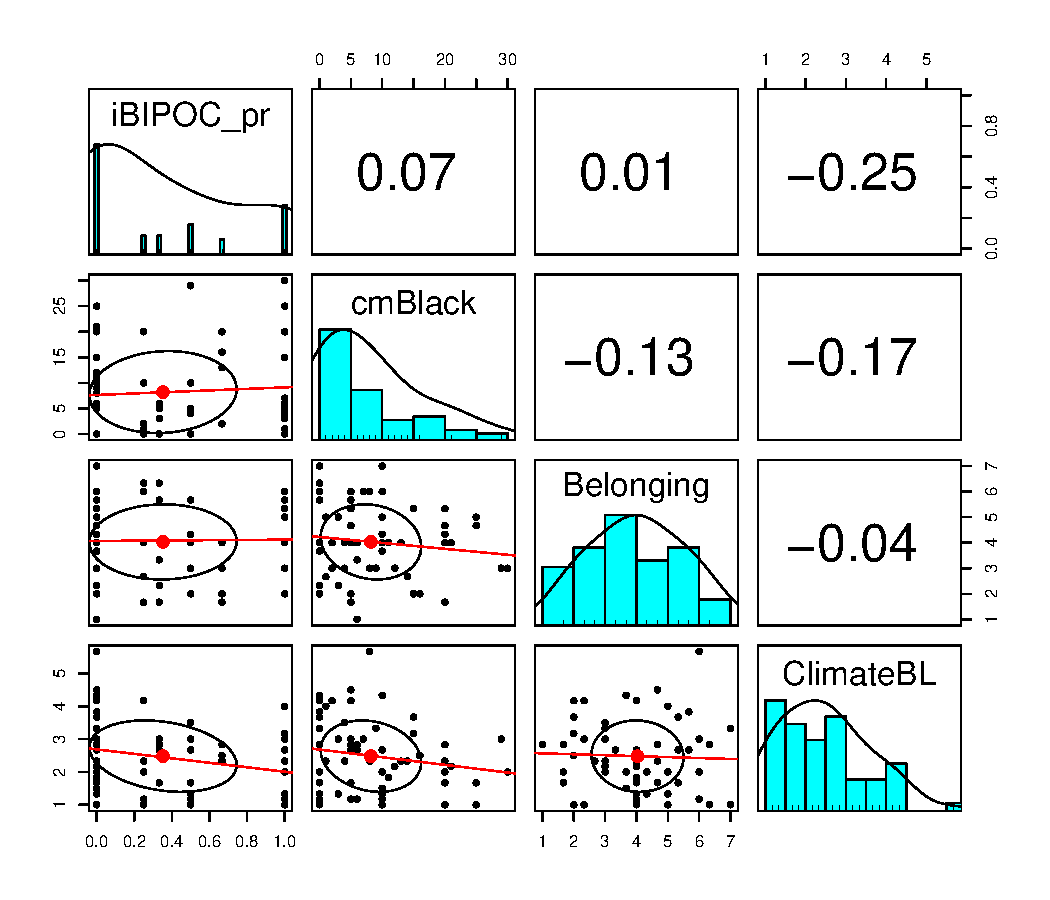
\includegraphics{03-DataDx_files/figure-latex/unnamed-chunk-11-1.pdf}

The histograms displayed in the diagonal graph for us what we learned from the Shapiro Wilk's test of normality. We can clearly see the non-normal distribution in the iBIPOC\_pr and cmBlack variables.

CUMULATIVE CAPTURE FOR THE APA STYLE WRITE-UP:

\begin{quote}
\begin{quote}
Regarding the distributional characteristics of the data, skew and kurtosis values of the variables fell below the values of 3 (skew) and 10 (kurtosis) that Kline suggests are concerning \citeyearpar{kline_principles_2016}. Results of the Shapiro-Wilk test of normality indicate that our variables assessing the proportion of classmates who are Black (\(W = 0.878, p < 0.001\)) and the proportion of BIPOC instructional staff(\(W = 0.787, p < 0.001\)) are statistically significantly different than a normal distribution. Similarly the scale assessing the respondent's perception of campus climate for Black students (\(W = 0.951, p = 0.016\)) differed significantly from a normal distribution. In all three cases the skew values and histograms suggested a somewhat positive skew. That is, there were predominantly low proportions of instructional staff who are BIPOC and classmates who are Black, and the perceptions of campus climate for Black students was evaluated somewhat favorably. The scales assessing the respondent's belonging (\(0.973, p = 0.165\)) did not differ significantly from a normal distribution.
\end{quote}
\end{quote}

What would we do in the case of a univariate outlier? I find Kline's \citeyearpar{kline_principles_2016} chapter on data preparation and management to be extremely useful. He provides ideas for more complex analysis of both univariate and multivariate normality and provides suggestions that range from recoding an extreme value to the next most extreme that is within three standard deviations of the mean to more complicated transformations. First, though we need to further examine the relationships between variables. We do that, next.

\hypertarget{evaluating-multivariate-normality}{%
\section{Evaluating Multivariate Normality}\label{evaluating-multivariate-normality}}

\textbf{Multivariate outliers} have extreme scores on two or more variables, or a pattern of scores that is atypical. For example, a case may have scores between two and three standard deviations above the mean on all variables, even though no case would be extreme. A common method of multivariate outlier detection is the \textbf{Mahalanobis distance} (\(D_{M}^{2}\)). This indicates the distance in variance units between the profile of scores for that case and the vector of sample means, or \textbf{centroid}, correcting for intercorrelations.

The \emph{outlier()} function from the \emph{psych} package tells us how far each datapoint is from the multivariate centroid of the data. That is, find the squared Mahalanobis distance for each data point and compare it to the expected values of \(\chi^2\). The \emph{outlier()} protocol also produces a Q-Q (quantile-quantile) plot with the \emph{n} most extreme data points labeled.

The code below appends the Mahalanobis values to the dataframe. It is easy, then, to identify, sort, and examine the most extreme values (relative to the rest of the data in their case/row) to make decisions about their retention or adjustment.

Numeric variables are required in the of the calculation of the Mahalanobis.

\begin{Shaded}
\begin{Highlighting}[]
\NormalTok{item\_scores\_df}\SpecialCharTok{$}\NormalTok{Mahal }\OtherTok{\textless{}{-}}\NormalTok{ psych}\SpecialCharTok{::}\FunctionTok{outlier}\NormalTok{(item\_scores\_df[}\FunctionTok{c}\NormalTok{(}\StringTok{"iBIPOC\_pr"}\NormalTok{, }\StringTok{"cmBlack"}\NormalTok{,}
    \StringTok{"Belonging"}\NormalTok{, }\StringTok{"ClimateBL"}\NormalTok{)])}
\end{Highlighting}
\end{Shaded}

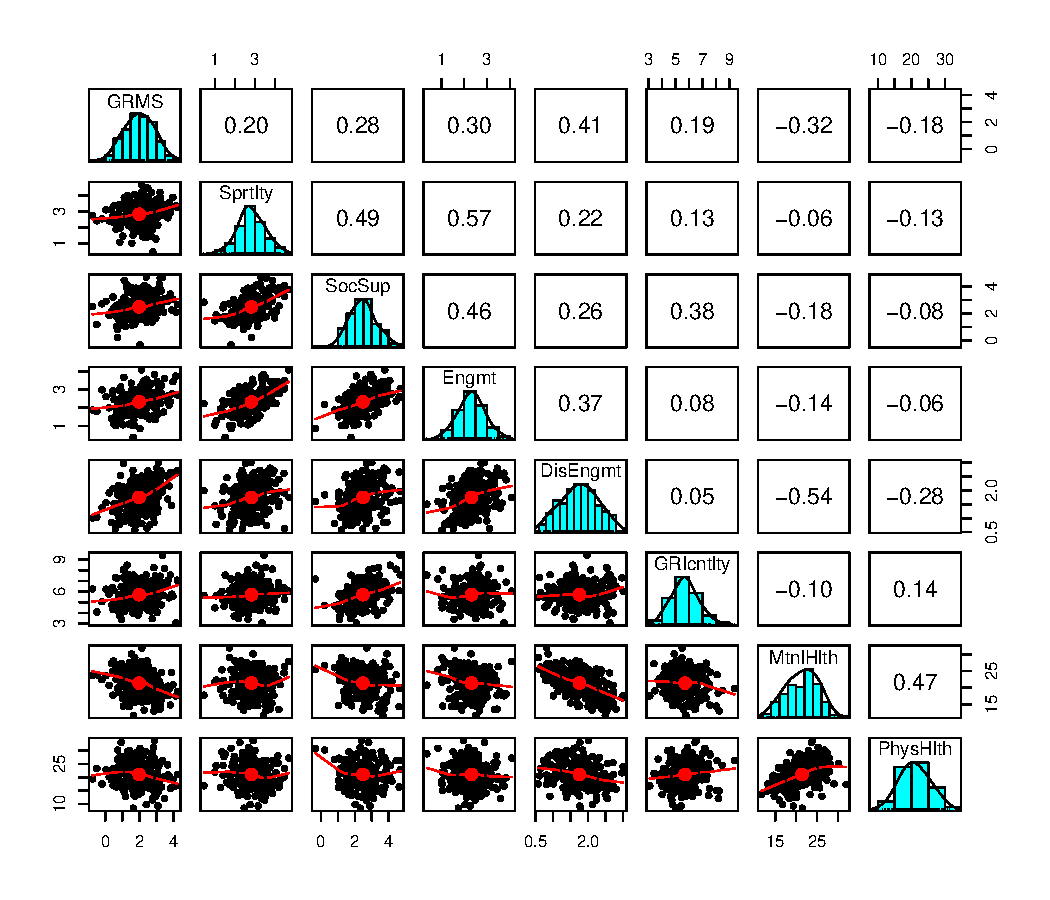
\includegraphics{03-DataDx_files/figure-latex/unnamed-chunk-12-1.pdf}

Q-Q plots take your sample data, sort it in ascending order, and then plot them versus quantiles (the number varies; you can see it on the X axis) calculated from a theoretical distribution. The number of quantiles is selected to match the size of your sample data. While Normal Q-Q Plots are the ones most often used in practice due to so many statistical methods assuming normality, Q-Q Plots can actually be created for any distribution. To the degree that the plotted line stays on the straight line (representing the theoretical normal distribution), the data is multivariate normally distributed.

It is possible, then to analyze the Mahalanobis distance values.

\begin{Shaded}
\begin{Highlighting}[]
\NormalTok{psych}\SpecialCharTok{::}\FunctionTok{describe}\NormalTok{(item\_scores\_df}\SpecialCharTok{$}\NormalTok{Mahal)}
\end{Highlighting}
\end{Shaded}

\begin{verbatim}
   vars  n mean   sd median trimmed  mad min   max range skew kurtosis   se
X1    1 66 3.81 2.24   3.68    3.62 2.36 0.2 11.25 11.05 0.86     0.82 0.28
\end{verbatim}

Using this information we can determine cases that have a Mahalanobis distance values that exceeds three standard deviations around the median. In fact, we can have these noted in a column in the dataframe.

\begin{Shaded}
\begin{Highlighting}[]
\CommentTok{\# creates a variable indicating TRUE or FALSE if an item is an}
\CommentTok{\# outlier}
\NormalTok{item\_scores\_df}\SpecialCharTok{$}\NormalTok{MOutlier }\OtherTok{\textless{}{-}}\NormalTok{ dplyr}\SpecialCharTok{::}\FunctionTok{if\_else}\NormalTok{(item\_scores\_df}\SpecialCharTok{$}\NormalTok{Mahal }\SpecialCharTok{\textgreater{}}\NormalTok{ (}\FunctionTok{median}\NormalTok{(item\_scores\_df}\SpecialCharTok{$}\NormalTok{Mahal) }\SpecialCharTok{+}
\NormalTok{    (}\DecValTok{3} \SpecialCharTok{*} \FunctionTok{sd}\NormalTok{(item\_scores\_df}\SpecialCharTok{$}\NormalTok{Mahal))), }\ConstantTok{TRUE}\NormalTok{, }\ConstantTok{FALSE}\NormalTok{)}

\CommentTok{\# shows us the first 6 rows of the data so we can see the new}
\CommentTok{\# variables (Mahal, MOutlier)}
\FunctionTok{head}\NormalTok{(item\_scores\_df)}
\end{Highlighting}
\end{Shaded}

\begin{verbatim}
# A tibble: 6 x 19
     ID iBIPOC_pr cmBlack Belong_1 Belong_2 Belong_3 Blst_1 Blst_2 Blst_3 Blst_4
  <int>     <dbl>   <dbl>    <dbl>    <dbl>    <dbl>  <dbl>  <dbl>  <dbl>  <dbl>
1     1     0.333       0        6        6        7      5      3      5      2
2     2     0           5        4        4        6      6      6      2      2
3     3     0.5        10       NA        3       NA     NA      5      2      2
4     4     0.333       6        5        3        2      2      2      2      2
5     5     1           5        4        4        4      6      1      1      1
6     6     0          20        5        6        5      5      1      1      2
# i 9 more variables: Blst_5 <dbl>, Blst_6 <dbl>, rBlst_1 <dbl>,
#   Belonging <dbl>, ResponseBL <dbl>, StigmaBL <dbl>, ClimateBL <dbl>,
#   Mahal <dbl>, MOutlier <lgl>
\end{verbatim}

\begin{Shaded}
\begin{Highlighting}[]
\FunctionTok{library}\NormalTok{(tidyverse)}
\end{Highlighting}
\end{Shaded}

\begin{verbatim}
-- Attaching core tidyverse packages ------------------------ tidyverse 2.0.0 --
v dplyr     1.1.2     v readr     2.1.4
v forcats   1.0.0     v stringr   1.5.0
v ggplot2   3.4.3     v tibble    3.2.1
v lubridate 1.9.2     v tidyr     1.3.0
v purrr     1.0.1     
-- Conflicts ------------------------------------------ tidyverse_conflicts() --
x dplyr::filter() masks stats::filter()
x dplyr::lag()    masks stats::lag()
i Use the conflicted package (<http://conflicted.r-lib.org/>) to force all conflicts to become errors
\end{verbatim}

\begin{Shaded}
\begin{Highlighting}[]
\CommentTok{\# counts frequency TRUE and FALSE indicating outlier or not}
\NormalTok{OutlierCount }\OtherTok{\textless{}{-}}\NormalTok{ item\_scores\_df }\SpecialCharTok{\%\textgreater{}\%}
\NormalTok{    dplyr}\SpecialCharTok{::}\FunctionTok{count}\NormalTok{(MOutlier)}

\CommentTok{\# calculating how many outliers a slightly different way}
\FunctionTok{nrow}\NormalTok{(item\_scores\_df) }\SpecialCharTok{{-}}\NormalTok{ OutlierCount}
\end{Highlighting}
\end{Shaded}

\begin{verbatim}
  MOutlier  n
1       66  1
2       65 65
\end{verbatim}

When we identify outliers we often ask if we should delete them or transform the data. A general rule of thumb is to look for ``jumps'' in the Mahalanobis distance values. If they are progressing steadily and there is no ``jump,'' researchers will often retain the outliers.

CUMULATIVE CAPTURE FOR THE APA STYLE WRITE-UP:

\begin{quote}
\begin{quote}
We evaluated multivariate normality with the Mahalanobis distance test. Specifically, we used the \emph{psych::outlier()} function and included all continuous variables in the calculation. Our visual inspection of the Q-Q plot suggested that the plotted line strayed from the straight line as the quantiles increased. Additionally, we appended the Mahalanobis distance scores as a variable to the data. Analyzing this variable, we found that 1 case exceed three standard deviations beyond the median. Given that the Mahalanobis distance values increased in a consistent manner (i.e., no extreme ``jumps'') we retained all cases.
\end{quote}
\end{quote}

\hypertarget{a-few-words-on-transformations}{%
\section{A Few Words on Transformations}\label{a-few-words-on-transformations}}

To quote from Kline \citeyearpar{kline_principles_2016}, ``Before applying a normalizing transformation, you should think about the variables of interest and whether the expectation of normality is reasonable.'' (p.~77)

At this point in history, the non-normal distribution of the proportions of classmates who are Black and instructional staff who are BIPOC are accurate representations in higher education. Kline \citeyearpar{kline_principles_2016} has noted that transforming an inherently non-normal variable to force a normal distribution may fundamentally alter it such that the variable of interest is not actually studied. Kline's chapter reviews some options for applying corrections to outliers. Additionally, the chapter describes a variety of normalizing transformations.

On a personal note, while I will use standardized scores (a linear transformation) if it improves interpretation and center variables around a meaningful intercept, I tend to resist the transformation of data without a really compelling reason. Why? It's complicated and can make interpretation difficult.

\hypertarget{the-apa-style-write-up-1}{%
\section{The APA Style Write-Up}\label{the-apa-style-write-up-1}}

This results section will draw from the three lessons on scrubbing, scoring, and data diagnostics.:

\hypertarget{data-diagnostics}{%
\subsection{Data Diagnostics}\label{data-diagnostics}}

\begin{quote}
\begin{quote}
Data screening suggested that 107 individuals opened the survey link. Of those, 83 granted consent and proceeded into the survey items. A further inclusion criteria was that the course was taught in the U.S; 69 met this criteria.
\end{quote}
\end{quote}

\begin{quote}
\begin{quote}
Available item analysis (AIA; \citep{parent_handling_2013}) is a strategy for managing missing data that uses available data for analysis and excludes cases with missing data points only for analyses in which the data points would be directly involved. Parent (2013) suggested that AIA is equivalent to more complex methods (e.g., multiple imputation) across a number of variations of sample size, magnitude of associations among items, and degree of missingness. Thus, we utilized Parent's recommendations to guide our approach to managing missing data. Missing data analyses were conducted with tools in base R as well as the R packages, \emph{psych} (v. 2.3.6) and \emph{mice} (v. 3.16.0).
\end{quote}
\end{quote}

\begin{quote}
\begin{quote}
Across cases that were deemed eligible on the basis of the inclusion/exclusion criteria, missingness ranged from 0 to 67\%. Across the dataset, 3.86\% of cells had missing data and 87.88\% of cases had nonmissing data. At this stage in the analysis, we allowed all cases with less than 90\% missing to continue to the scoring stage. Guided by Parent's \citeyearpar{parent_handling_2013} AIA approach, scales with three items were scored if at least two items were non-missing; the scale with four items was scored if it at least three non-missing items; and the scale with six items was scored if it had at least five non-missing items.
\end{quote}
\end{quote}

\begin{quote}
\begin{quote}
Across the 66 cases for which the scoring protocol was applied, missingness ranged from 0 to 67\%. After eliminating cases with greater than 20\% missing, the dataset analyzed included 61 cases. In this dataset we had less than 1\% (0.55\%) missing across the df; 97\% of the rows had nonmissing data.
\end{quote}
\end{quote}

\begin{quote}
\begin{quote}
Regarding the distributional characteristics of the data, skew and kurtosis values of the variables fell below the values of 3 (skew) and 10 (kurtosis) that Kline suggests are concerning \citeyearpar{kline_principles_2016}. Results of the Shapiro-Wilk test of normality indicate that our variables assessing the proportion of classmates who are Black (\(W = 0.878, p < 0.001\)) and the proportion of BIPOC instructional staff(\(W = 0.787, p < 0.001\)) are statistically significantly different than a normal distribution. The scales assessing the respondent's belonging (\(0.973, p = 0.165\)) and the respondent's perception of campus climate for Black students (\(W = 0.951, p = 0.016\)) did not differ differently from a normal distribution.
\end{quote}
\end{quote}

\begin{quote}
\begin{quote}
We evaluated multivariate normality with the Mahalanobis distance test. Specifically, we used the \emph{psych::outlier()} function and included all continuous variables in the calculation. Our visual inspection of the Q-Q plot suggested that the plotted line strayed from the straight line as the quantiles increased. Additionally, we appended the Mahalanobis distance scores as a variable to the data. Analyzing this variable, we found that 1 case exceed three standard deviations beyond the median. Given that the Mahalanobis distance values increased in a consistent manner (i.e., no extreme ``jumps'') we retained all cases.
\end{quote}
\end{quote}

\begin{quote}
\begin{quote}
Given that our sample sizes were reasonable for the planned analyses and the degree of missingness was low, we used pairwise deletion in our multiple regression analysis.
\end{quote}
\end{quote}

\hypertarget{a-quick-regression-of-our-research-vignette}{%
\section{A Quick Regression of our Research Vignette}\label{a-quick-regression-of-our-research-vignette}}

With some confidence that our scrubbed-and-scored variables are appropriate for analysis, let me conduct the super quick regression that is our research vignette.

\begin{figure}
\centering
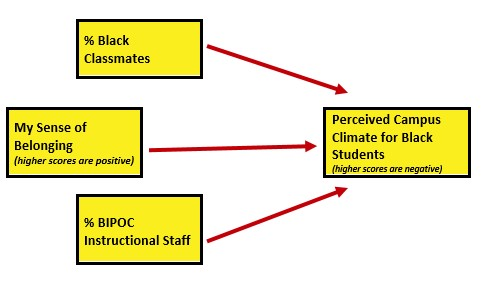
\includegraphics{images/Ch04/BlStuRegression.jpg}
\caption{An image of the statistical model for which we are preparing data.}
\end{figure}

\begin{Shaded}
\begin{Highlighting}[]
\NormalTok{Climate\_fit }\OtherTok{\textless{}{-}} \FunctionTok{lm}\NormalTok{(ClimateBL }\SpecialCharTok{\textasciitilde{}}\NormalTok{ Belonging }\SpecialCharTok{+}\NormalTok{ cmBlack }\SpecialCharTok{+}\NormalTok{ iBIPOC\_pr, }\AttributeTok{data =}\NormalTok{ item\_scores\_df)}
\FunctionTok{summary}\NormalTok{(Climate\_fit)}
\end{Highlighting}
\end{Shaded}

\begin{verbatim}

Call:
lm(formula = ClimateBL ~ Belonging + cmBlack + iBIPOC_pr, data = item_scores_df)

Residuals:
     Min       1Q   Median       3Q      Max 
-1.86732 -0.80535  0.02355  0.70459  3.02003 

Coefficients:
            Estimate Std. Error t value     Pr(>|t|)    
(Intercept)  2.90791    0.46653   6.233 0.0000000674 ***
Belonging   -0.01742    0.09643  -0.181        0.857    
cmBlack     -0.01918    0.01717  -1.117        0.269    
iBIPOC_pr   -0.64125    0.35701  -1.796        0.078 .  
---
Signif. codes:  0 '***' 0.001 '**' 0.01 '*' 0.05 '.' 0.1 ' ' 1

Residual standard error: 1.066 on 55 degrees of freedom
  (7 observations deleted due to missingness)
Multiple R-squared:  0.08212,   Adjusted R-squared:  0.03206 
F-statistic:  1.64 on 3 and 55 DF,  p-value: 0.1906
\end{verbatim}

\hypertarget{results-1}{%
\subsection{Results}\label{results-1}}

\begin{quote}
\begin{quote}
Results of a multiple regression predicting the respondents' perceptions of campus climate for Black students indicated that neither contributions of the respondents' personal belonging (\(B = -0.017, p = -.857\)), the proportion of BIPOC instructional staff (\(B-0.641, p = 0.078), nor the proportion of Black classmates (\)B\$ = -0.019, p = 0.269 ) led to statistically significant changes in perceptions of campus climate for Black students. The model accounted for only 8\% of the variance and was not statistically significant (\(p = 0.191\)). Means, standard deviations, and correlations among variables are presented in Table 1; results of the regression model are presented in Table 2.
\end{quote}
\end{quote}

\begin{Shaded}
\begin{Highlighting}[]
\NormalTok{apaTables}\SpecialCharTok{::}\FunctionTok{apa.cor.table}\NormalTok{(item\_scores\_df[}\FunctionTok{c}\NormalTok{(}\StringTok{"iBIPOC\_pr"}\NormalTok{, }\StringTok{"cmBlack"}\NormalTok{, }\StringTok{"Belonging"}\NormalTok{,}
    \StringTok{"ClimateBL"}\NormalTok{)], }\AttributeTok{table.number =} \DecValTok{1}\NormalTok{, }\AttributeTok{show.sig.stars =} \ConstantTok{TRUE}\NormalTok{, }\AttributeTok{filename =} \StringTok{"Table1\_M\_SDs\_r\_DataDx.doc"}\NormalTok{)}
\end{Highlighting}
\end{Shaded}

\begin{verbatim}


Table 1 

Means, standard deviations, and correlations with confidence intervals
 

  Variable     M    SD   1           2           3          
  1. iBIPOC_pr 0.35 0.39                                    
                                                            
  2. cmBlack   8.20 8.02 .07                                
                         [-.18, .31]                        
                                                            
  3. Belonging 4.03 1.47 .01         -.13                   
                         [-.24, .26] [-.36, .12]            
                                                            
  4. ClimateBL 2.48 1.09 -.25        -.17        -.04       
                         [-.47, .01] [-.41, .08] [-.29, .22]
                                                            

Note. M and SD are used to represent mean and standard deviation, respectively.
Values in square brackets indicate the 95% confidence interval.
The confidence interval is a plausible range of population correlations 
that could have caused the sample correlation (Cumming, 2014).
 * indicates p < .05. ** indicates p < .01.
 
\end{verbatim}

\begin{Shaded}
\begin{Highlighting}[]
\FunctionTok{library}\NormalTok{(apaTables)}
\NormalTok{apaTables}\SpecialCharTok{::}\FunctionTok{apa.reg.table}\NormalTok{(Climate\_fit, }\AttributeTok{table.number =} \DecValTok{2}\NormalTok{, }\AttributeTok{filename =} \StringTok{"Climate\_table.doc"}\NormalTok{)}
\end{Highlighting}
\end{Shaded}

\begin{verbatim}


Table 2 

Regression results using ClimateBL as the criterion
 

   Predictor      b      b_95%_CI  beta   beta_95%_CI sr2  sr2_95%_CI    r
 (Intercept) 2.91**  [1.97, 3.84]                                         
   Belonging  -0.02 [-0.21, 0.18] -0.02 [-0.28, 0.24] .00 [-.01, .01] -.00
     cmBlack  -0.02 [-0.05, 0.02] -0.15 [-0.41, 0.12] .02 [-.05, .09] -.17
   iBIPOC_pr  -0.64 [-1.36, 0.07] -0.23 [-0.49, 0.03] .05 [-.06, .16] -.25
                                                                          
                                                                          
                                                                          
             Fit
                
                
                
                
       R2 = .082
 95% CI[.00,.20]
                

Note. A significant b-weight indicates the beta-weight and semi-partial correlation are also significant.
b represents unstandardized regression weights. beta indicates the standardized regression weights. 
sr2 represents the semi-partial correlation squared. r represents the zero-order correlation.
Square brackets are used to enclose the lower and upper limits of a confidence interval.
* indicates p < .05. ** indicates p < .01.
 
\end{verbatim}

\hypertarget{practice-problems-2}{%
\section{Practice Problems}\label{practice-problems-2}}

The three problems described below are designed to be continuations from the Scrubbing and Scoring lessons. You will likely encounter challenges that were not covered in this chapter. Search for and try out solutions, knowing that there are multiple paths through the analysis. The overall notion of the suggestions for practice are to (a) calculate alpha coefficients for the scales, (b) evaluate univariate and multivariate normality, (c) create an APA-style write-up appropriate for a data diagnostics subsection of the results, and (d) run a ``quickie'' regression, ANOVA, or similar analysis.

\hypertarget{problem-1-reworking-the-chapter-problem-1}{%
\subsection{Problem \#1: Reworking the Chapter Problem}\label{problem-1-reworking-the-chapter-problem-1}}

If you chose this option in the prior chapters, you imported the data from Qualtrics, applied inclusion/exclusion criteria, renamed variables, downsized the df to the variables of interest, properly formatted the variables, interpreted item-level missingness, scored the scales/subscales, interpreted scale-level missingness, and wrote up the results. Please continue with the remaining tasks.

\hypertarget{problem-2-use-the-rate-a-recent-course-survey-choosing-different-variables-2}{%
\subsection{\texorpdfstring{Problem \#2: Use the \emph{Rate-a-Recent-Course} Survey, Choosing Different Variables}{Problem \#2: Use the Rate-a-Recent-Course Survey, Choosing Different Variables}}\label{problem-2-use-the-rate-a-recent-course-survey-choosing-different-variables-2}}

If you chose this option in the prior chapter, you chose a minimum of three variables (different from those in the cahpter) from the \emph{Rate-a-Recent-Course} survey to include in a simple statistical model. You imported the data from Qualtrics, applied inclusion/exclusion criteria, renamed variables, downsized the df to the variables of interest, properly formatted the variables, interpreted item-level missingness, scored the scales/subscales, interpreted scale-level missingness, and wrote up the results. Please continue with the remaining tasks.

\hypertarget{problem-3-other-data-2}{%
\subsection{Problem \#3: Other data}\label{problem-3-other-data-2}}

If you chose this option in the prior chapter, you used raw data that was available to you. You imported it into R, applied inclusion/exclusion criteria, renamed variables, downsized the df to the variables of interest, properly formatted the variables, interpreted item-level missingness, scored the scales/subscales, interpreted scale-level missingness, and wrote up the results. Please continue with the remaining tasks.

\hypertarget{grading-rubric-2}{%
\subsection{Grading Rubric}\label{grading-rubric-2}}

\begin{longtable}[]{@{}
  >{\raggedright\arraybackslash}p{(\columnwidth - 4\tabcolsep) * \real{0.7642}}
  >{\centering\arraybackslash}p{(\columnwidth - 4\tabcolsep) * \real{0.1220}}
  >{\centering\arraybackslash}p{(\columnwidth - 4\tabcolsep) * \real{0.1138}}@{}}
\toprule\noalign{}
\begin{minipage}[b]{\linewidth}\raggedright
Assignment Component
\end{minipage} & \begin{minipage}[b]{\linewidth}\centering
\end{minipage} & \begin{minipage}[b]{\linewidth}\centering
\end{minipage} \\
\midrule\noalign{}
\endhead
\bottomrule\noalign{}
\endlastfoot
1. Calculate alpha coefficients for scales/subscales. & 5 & \_\_\_\_\_ \\
2. Evaluate univariate normality (skew, kurtosis, Shapiro-Wilks). & 5 & \_\_\_\_\_ \\
3. Evaluate multivariate normality (Mahalanobis test) & 5 & \_\_\_\_\_ \\
4. Represent your work in an APA-style write-up (added to the writeup in the previous chapter) & 5 & \_\_\_\_\_ \\
5. Conduct a quick analysis (e.g., regression, ANOVA) including at least three predictor variables & 5 & \_\_\_\_\_ \\
6. Explanation to grader & 5 & \_\_\_\_\_ \\
\textbf{Totals} & 30 & \_\_\_\_\_ \\
\end{longtable}

\hypertarget{homeworked-example}{%
\section{Homeworked Example}\label{homeworked-example}}

\href{}{Screencast Link}

For more information about the data used in this homeworked example, please refer to the description and codebook located at the end of the \href{https://lhbikos.github.io/ReCenterPsychStats/ReCintro.html\#introduction-to-the-data-set-used-for-homeworked-examples}{introductory lesson} in \href{https://lhbikos.github.io/ReCenterPsychStats/}{ReCentering Psych Stats}. An .rds file which holds the data is located in the \href{https://github.com/lhbikos/ReC_MultivModel/tree/main/Worked_Examples}{Worked Examples} folder at the GitHub site the hosts the OER. The file name is \emph{ReC.rds}.

Although the lessons focused on preparing data for analyses were presented in smaller sections, this homeworked example combines the suggestions for practice from the \protect\hyperlink{scrub}{Scrubbing}, \protect\hyperlink{scrub}{Scoring}, and \protect\hyperlink{datadx}{Data Dx} lessons. My hope is that is cumulative presentation is a closer approximation of what researchers need for their research projects.

These lessons were created to prepare a set of data to analyze a specific research model. Consequently, the model should be known and described at the beginning.

\hypertarget{scrubbing-1}{%
\subsection{Scrubbing}\label{scrubbing-1}}

\hypertarget{specify-a-research-model}{%
\subsubsection*{Specify a research model}\label{specify-a-research-model}}


A further requirement was that the model should include three predictor variables (continuously or categorically scaled) and one dependent (continuously scaled) variable.

I am hypothesizing that socially responsive pedagogy (my dependent variable) will increase as a function of:

\begin{itemize}
\tightlist
\item
  the transition from SPSS (0) to R(1),
\item
  the transition from a pre-centered (0) to re-centered (1) curriculum, and
\item
  higher evaluations of traditional pedagogy
\end{itemize}

Because this data is nested within the person (i.e., students can contribute up to three course evaluations over the ANOVA, multivariate, and psychometrics courses) proper analysis would require a statistic (e.g., multilevel modeling) that would address the dependency in the data. Therefore, I will include only those students who are taking the multivariate modeling class.

\emph{If you wanted to use this example and dataset as a basis for a homework assignment, you could create a different subset of data. I worked the example for students taking the multivariate modeling class. You could choose ANOVA or psychometrics. You could also choose a different combinations of variables.}

\begin{figure}
\centering
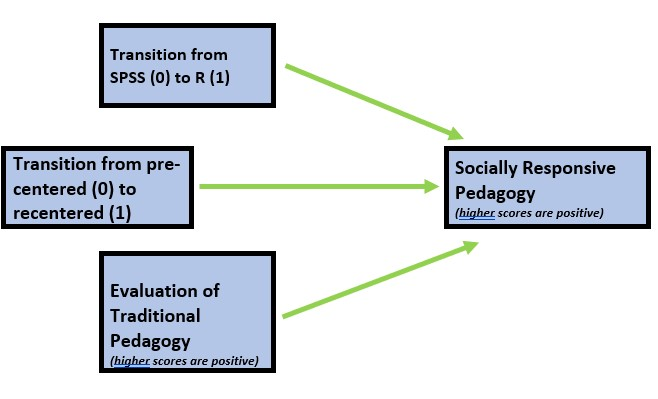
\includegraphics{Worked_Examples/images/homeworked_model.jpg}
\caption{An image of our the prediction model for the homeworked example.}
\end{figure}

\hypertarget{import-data}{%
\subsubsection*{Import data}\label{import-data}}


\begin{Shaded}
\begin{Highlighting}[]
\NormalTok{raw }\OtherTok{\textless{}{-}} \FunctionTok{readRDS}\NormalTok{(}\StringTok{"ReC.rds"}\NormalTok{)}
\FunctionTok{nrow}\NormalTok{(raw)}
\end{Highlighting}
\end{Shaded}

\begin{verbatim}
[1] 310
\end{verbatim}

\hypertarget{include-only-those-who-consented}{%
\subsubsection*{Include only those who consented}\label{include-only-those-who-consented}}


Because this data is publicly posted on the Open Science Framework, it was necessary for me to already exclude those individuals. This data was unique in that students could freely write some version of ``Opt out.'' My original code included a handful of versions, but here was the basic form:

\begin{Shaded}
\begin{Highlighting}[]
\CommentTok{\# testing to see if my code worked raw \textless{}{-} dplyr::filter (raw,}
\CommentTok{\# SPFC.Decolonize.Opt.Out != \textquotesingle{}Okay\textquotesingle{})}
\NormalTok{raw }\OtherTok{\textless{}{-}}\NormalTok{ dplyr}\SpecialCharTok{::}\FunctionTok{filter}\NormalTok{(raw, SPFC.Decolonize.Opt.Out }\SpecialCharTok{!=} \StringTok{"Opt Out"}\NormalTok{)}
\end{Highlighting}
\end{Shaded}

\hypertarget{apply-exclusionary-criteria}{%
\subsubsection*{Apply exclusionary criteria}\label{apply-exclusionary-criteria}}


I want to exclude students' responses for the ANOVA and psychometrics courses.

\begin{Shaded}
\begin{Highlighting}[]
\NormalTok{raw }\OtherTok{\textless{}{-}}\NormalTok{ (dplyr}\SpecialCharTok{::}\FunctionTok{filter}\NormalTok{(raw, Course }\SpecialCharTok{==} \StringTok{"Multivariate"}\NormalTok{))}
\end{Highlighting}
\end{Shaded}

At this point, these my only inclusion/exclusion criteria. I can determine how many students (who consented) completed any portion of the survey.

\begin{Shaded}
\begin{Highlighting}[]
\FunctionTok{nrow}\NormalTok{(raw)}
\end{Highlighting}
\end{Shaded}

\begin{verbatim}
[1] 84
\end{verbatim}

\hypertarget{rename-variables-to-be-sensible-and-systematic}{%
\subsubsection*{Rename variables to be sensible and systematic}\label{rename-variables-to-be-sensible-and-systematic}}


Because this dataset is already on the OSF, the variables are sensibly named. However, I don't like ``SPFC.Decolonize.Opt.Out''. I will change it to simply ``OptOut.''

\begin{Shaded}
\begin{Highlighting}[]
\NormalTok{raw }\OtherTok{\textless{}{-}}\NormalTok{ dplyr}\SpecialCharTok{::}\FunctionTok{rename}\NormalTok{(raw, }\AttributeTok{OptOut =} \StringTok{"SPFC.Decolonize.Opt.Out"}\NormalTok{)}
\end{Highlighting}
\end{Shaded}

It would have made more sense to do this before I used this variable in the calculations.

\hypertarget{downsize-the-dataframe-to-the-variables-of-interest}{%
\subsubsection*{Downsize the dataframe to the variables of interest}\label{downsize-the-dataframe-to-the-variables-of-interest}}


I will need to include:

\begin{itemize}
\tightlist
\item
  deID
\item
  StatsPkg
\item
  Centering
\item
  Items included in the traditional pedagogy scale: ClearResponsibilities, EffectiveAnswers, Feedback, ClearOrganization, ClearPresentation
\item
  Items included in the socially responsive pedagogy scale: InclusvClassrm, EquitableEval, MultPerspectives, DEIintegration
\end{itemize}

\begin{Shaded}
\begin{Highlighting}[]
\NormalTok{scrub\_df }\OtherTok{\textless{}{-}}\NormalTok{ (dplyr}\SpecialCharTok{::}\FunctionTok{select}\NormalTok{(raw, deID, StatsPkg, Centering, ClearResponsibilities,}
\NormalTok{    EffectiveAnswers, Feedback, ClearOrganization, ClearPresentation, InclusvClassrm,}
\NormalTok{    EquitableEval, MultPerspectives, DEIintegration))}
\end{Highlighting}
\end{Shaded}

\hypertarget{provide-an-apa-style-write-up-of-these-preliminary-steps}{%
\subsubsection*{Provide an APA style write-up of these preliminary steps}\label{provide-an-apa-style-write-up-of-these-preliminary-steps}}


\begin{quote}
\begin{quote}
This is a secondary analysis of data involved in a more comprehensive dataset that included students taking multiple statistics courses (\emph{N} = 310). Having retrieved this data from a repository in the Open Science Framework, only those who consented to participation in the study were included. Data used in these analyses were 84 students who completed the multivariate class.
\end{quote}
\end{quote}

\hypertarget{scoring-1}{%
\subsection{Scoring}\label{scoring-1}}

\hypertarget{proper-formatting-of-the-items-in-your-first-predictor-variable}{%
\subsubsection*{Proper formatting of the item(s) in your first predictor variable}\label{proper-formatting-of-the-items-in-your-first-predictor-variable}}


StatsPkg is a dichotomous variable. It should be structured as a factor with two ordered levels: SPSS, R

Because I am using the .rds form of the data from the OSF, this variable retains the former structure I assigned to it. If I needed to write the code, I would do this:

\begin{Shaded}
\begin{Highlighting}[]
\NormalTok{scrub\_df}\SpecialCharTok{$}\NormalTok{StatsPkg }\OtherTok{\textless{}{-}} \FunctionTok{factor}\NormalTok{(scrub\_df}\SpecialCharTok{$}\NormalTok{StatsPkg, }\AttributeTok{levels =} \FunctionTok{c}\NormalTok{(}\StringTok{"SPSS"}\NormalTok{, }\StringTok{"R"}\NormalTok{))}
\FunctionTok{str}\NormalTok{(scrub\_df}\SpecialCharTok{$}\NormalTok{StatsPkg)}
\end{Highlighting}
\end{Shaded}

\begin{verbatim}
 Factor w/ 2 levels "SPSS","R": 2 2 2 2 2 2 2 2 2 2 ...
\end{verbatim}

\hypertarget{proper-formatting-of-items-in-your-second-predictor-variable}{%
\subsubsection*{Proper formatting of item(s) in your second predictor variable}\label{proper-formatting-of-items-in-your-second-predictor-variable}}


Similarly, Centering is a dichotomous variable. It should be structured as a factor with two ordered levels: Pre, Re.

Because I am using the .rds form of the data from the OSF, this variable retains the former structure I assigned to it. If I needed to write the code, I would do this:

\begin{Shaded}
\begin{Highlighting}[]
\NormalTok{scrub\_df}\SpecialCharTok{$}\NormalTok{Centering }\OtherTok{\textless{}{-}} \FunctionTok{factor}\NormalTok{(scrub\_df}\SpecialCharTok{$}\NormalTok{Centering, }\AttributeTok{levels =} \FunctionTok{c}\NormalTok{(}\StringTok{"Pre"}\NormalTok{, }\StringTok{"Re"}\NormalTok{))}
\FunctionTok{str}\NormalTok{(scrub\_df}\SpecialCharTok{$}\NormalTok{Centering)}
\end{Highlighting}
\end{Shaded}

\begin{verbatim}
 Factor w/ 2 levels "Pre","Re": 2 2 2 2 2 2 2 2 2 2 ...
\end{verbatim}

\hypertarget{proper-formatting-of-the-items-in-your-third-predictor-variable}{%
\subsubsection*{Proper formatting of the item(s) in your third predictor variable}\label{proper-formatting-of-the-items-in-your-third-predictor-variable}}


\hypertarget{proper-formatting-of-the-items-in-your-dependent-variable}{%
\subsubsection*{Proper formatting of the item(s) in your dependent variable}\label{proper-formatting-of-the-items-in-your-dependent-variable}}


The third predictor variable is traditional pedagogy. The dependent variable is socially repsonsive pedagogy. The items that will be used in the scale scores for both of these variables are all continuously scaled and should be identified as ``int'' or ``num.'' None of the items need to be reverse-scored.

\begin{Shaded}
\begin{Highlighting}[]
\FunctionTok{str}\NormalTok{(scrub\_df)}
\end{Highlighting}
\end{Shaded}

\begin{verbatim}
Classes 'data.table' and 'data.frame':  84 obs. of  12 variables:
 $ deID                 : int  11 12 13 14 15 16 17 18 35 19 ...
 $ StatsPkg             : Factor w/ 2 levels "SPSS","R": 2 2 2 2 2 2 2 2 2 2 ...
 $ Centering            : Factor w/ 2 levels "Pre","Re": 2 2 2 2 2 2 2 2 2 2 ...
 $ ClearResponsibilities: int  4 5 5 5 4 3 5 5 3 5 ...
 $ EffectiveAnswers     : int  4 5 5 4 4 3 5 5 4 4 ...
 $ Feedback             : int  4 5 4 4 5 4 5 4 4 5 ...
 $ ClearOrganization    : int  3 5 5 4 4 3 5 5 4 5 ...
 $ ClearPresentation    : int  4 5 5 3 4 2 5 4 5 5 ...
 $ InclusvClassrm       : int  5 5 5 5 5 4 5 5 5 5 ...
 $ EquitableEval        : int  4 5 5 5 4 4 5 4 5 5 ...
 $ MultPerspectives     : int  4 5 5 5 5 5 5 4 5 5 ...
 $ DEIintegration       : int  5 5 5 5 5 5 5 5 5 5 ...
 - attr(*, ".internal.selfref")=<externalptr> 
\end{verbatim}

\hypertarget{evaluate-and-interpret-item-level-missingness}{%
\subsubsection*{Evaluate and interpret item-level missingness}\label{evaluate-and-interpret-item-level-missingness}}


The \emph{scrub\_df} is already downsized to include the item-level raw variables and the ID variable. We can continue using it.

I will create a ``proportion missing'' variable.

In this chunk I first calculate the number of missing (nmiss)

\begin{Shaded}
\begin{Highlighting}[]
\FunctionTok{library}\NormalTok{(tidyverse)}\CommentTok{\#needed because the script has pipes}

\CommentTok{\#Calculating number and proportion of item{-}level missingness}
\NormalTok{scrub\_df}\SpecialCharTok{$}\NormalTok{nmiss }\OtherTok{\textless{}{-}}\NormalTok{ scrub\_df}\SpecialCharTok{\%\textgreater{}\%}
\NormalTok{    dplyr}\SpecialCharTok{::}\FunctionTok{select}\NormalTok{(StatsPkg}\SpecialCharTok{:}\NormalTok{DEIintegration) }\SpecialCharTok{\%\textgreater{}\%} \CommentTok{\#the colon allows us to include all variables between the two listed (the variables need to be in order)}
\NormalTok{    is.na }\SpecialCharTok{\%\textgreater{}\%} 
\NormalTok{    rowSums}

\NormalTok{scrub\_df}\OtherTok{\textless{}{-}}\NormalTok{ scrub\_df}\SpecialCharTok{\%\textgreater{}\%}
\NormalTok{  dplyr}\SpecialCharTok{::}\FunctionTok{mutate}\NormalTok{(}\AttributeTok{prop\_miss =}\NormalTok{ (nmiss}\SpecialCharTok{/}\DecValTok{11}\NormalTok{)}\SpecialCharTok{*}\DecValTok{100}\NormalTok{) }\CommentTok{\#11 is the number of variables included in calculating the proportion}
\end{Highlighting}
\end{Shaded}

We can grab the descriptives for the \emph{prop\_miss} variable to begin to understand our data. I will create an object from it so I can use it with inline

\begin{Shaded}
\begin{Highlighting}[]
\NormalTok{psych}\SpecialCharTok{::}\FunctionTok{describe}\NormalTok{(scrub\_df}\SpecialCharTok{$}\NormalTok{prop\_miss)}
\end{Highlighting}
\end{Shaded}

\begin{verbatim}
   vars  n mean   sd median trimmed mad min   max range skew kurtosis   se
X1    1 84 2.38 6.17      0    0.94   0   0 36.36 36.36 3.29    12.33 0.67
\end{verbatim}

Because I want to use the AIA approach to scoring, I'm not willing to filter out any cases yet. If I wanted to eliminate cases with egregious missing (i.e., like 90\%), here is the code I would use:

\begin{Shaded}
\begin{Highlighting}[]
\NormalTok{scrub\_df }\OtherTok{\textless{}{-}}\NormalTok{ dplyr}\SpecialCharTok{::}\FunctionTok{filter}\NormalTok{(scrub\_df, prop\_miss }\SpecialCharTok{\textless{}=} \DecValTok{90}\NormalTok{)  }\CommentTok{\#update df to have only those with at least 90\% of complete data}
\end{Highlighting}
\end{Shaded}

CUMULATIVE CAPTURE FOR WRITING IT UP:

\begin{quote}
\begin{quote}
Across cases that were deemed eligible on the basis of the inclusion/exclusion criteria, missingness ranged from 0 to 36\%.
\end{quote}
\end{quote}

To analyze missingness at the item level, we need a df that has only the variables of interest. That is, variables like \emph{ID} and the \emph{prop\_miss} and \emph{nmiss} variables we created will interfere with an accurate assessment of missingness. I will update our df to eliminate these.

\begin{Shaded}
\begin{Highlighting}[]
\CommentTok{\# further update to exclude the n\_miss and prop\_miss variables}
\NormalTok{ItemMiss\_df }\OtherTok{\textless{}{-}}\NormalTok{ scrub\_df }\SpecialCharTok{\%\textgreater{}\%}
\NormalTok{    dplyr}\SpecialCharTok{::}\FunctionTok{select}\NormalTok{(}\SpecialCharTok{{-}}\FunctionTok{c}\NormalTok{(deID, nmiss, prop\_miss))}
\end{Highlighting}
\end{Shaded}

Missing data analysis commonly looks at proportions by:

\begin{itemize}
\tightlist
\item
  the entire df
\item
  rows/cases/people
\end{itemize}

\begin{Shaded}
\begin{Highlighting}[]
\CommentTok{\# what proportion of cells missing across entire dataset}
\NormalTok{formattable}\SpecialCharTok{::}\FunctionTok{percent}\NormalTok{(}\FunctionTok{mean}\NormalTok{(}\FunctionTok{is.na}\NormalTok{(ItemMiss\_df)))}
\end{Highlighting}
\end{Shaded}

\begin{verbatim}
[1] 2.38%
\end{verbatim}

\begin{Shaded}
\begin{Highlighting}[]
\CommentTok{\# what proportion of cases (rows) are complete (nonmissing)}
\NormalTok{formattable}\SpecialCharTok{::}\FunctionTok{percent}\NormalTok{(}\FunctionTok{mean}\NormalTok{(}\FunctionTok{complete.cases}\NormalTok{(ItemMiss\_df)))}
\end{Highlighting}
\end{Shaded}

\begin{verbatim}
[1] 82.14%
\end{verbatim}

CUMULATIVE CAPTURE FOR WRITING IT UP:

\begin{quote}
\begin{quote}
Across cases that were deemed eligible on the basis of the inclusion/exclusion criteria, missingness ranged from 0 to 36\%. Across the dataset, 2.38\% of cells had missing data and 82.14\% of cases had nonmissing data.
\end{quote}
\end{quote}

We can further explore patterns of missingness with \emph{mice.md.pattern}.

\begin{Shaded}
\begin{Highlighting}[]
\NormalTok{mice}\SpecialCharTok{::}\FunctionTok{md.pattern}\NormalTok{(ItemMiss\_df, }\AttributeTok{plot =} \ConstantTok{TRUE}\NormalTok{, }\AttributeTok{rotate.names =} \ConstantTok{TRUE}\NormalTok{)}
\end{Highlighting}
\end{Shaded}

There are 6 missingness patterns. The most common (\emph{n} = 69) have no missingness. There are 11 students missing the DEIintegration item (on the traditional pedagogy scale). This item may have been a later addition to the Canvas course evaluations.

Comparing this to Enders' \citeyearpar{enders_applied_2010} \href{https://www.google.com/books/edition/Applied_Missing_Data_Analysis/uHt4EAAAQBAJ?hl=en\&gbpv=1\&dq=enders+missing+data\&pg=PP1\&printsec=frontcover}{prototypical patterns of missingness} (page 3), the \emph{mice} output represents the monotonic pattern often caused by test fatigue. That is, once a student stopped responding, they didn't continue with the rest of the evaluation. That said, this was true of only 4 students (1 each pattern). A quick reminder -- diagnosing monotonicity requires that the variables in the \emph{mice.mdpattern} figures were presented to the research participant in that order.

\hypertarget{score-any-scalessubscales}{%
\subsubsection*{Score any scales/subscales}\label{score-any-scalessubscales}}


Traditional pedagogy is a predictor variable that needs to be created by calculating the mean if at least 75\% of the items are non-missing. None of the items need to be reverse-scored. I will return to working with the \emph{scrub\_df} data.

\begin{Shaded}
\begin{Highlighting}[]
\CommentTok{\# this seems to work when I build the book, but not in \textquotesingle{}working the}
\CommentTok{\# problem\textquotesingle{} TradPed\_vars \textless{}{-} c(\textquotesingle{}ClearResponsibilities\textquotesingle{},}
\CommentTok{\# \textquotesingle{}EffectiveAnswers\textquotesingle{},\textquotesingle{}Feedback\textquotesingle{},}
\CommentTok{\# \textquotesingle{}ClearOrganization\textquotesingle{},\textquotesingle{}ClearPresentation\textquotesingle{}) scrub\_df$TradPed \textless{}{-}}
\CommentTok{\# sjstats::mean\_n(scrub\_df[, TradPed\_vars], .75)}

\CommentTok{\# this seems to work when I \textquotesingle{}work the problem\textquotesingle{} (but not when I build}
\CommentTok{\# the book) the difference is the two dots before the last SRPed\_vars}
\NormalTok{TradPed\_vars }\OtherTok{\textless{}{-}} \FunctionTok{c}\NormalTok{(}\StringTok{"ClearResponsibilities"}\NormalTok{, }\StringTok{"EffectiveAnswers"}\NormalTok{, }\StringTok{"Feedback"}\NormalTok{,}
    \StringTok{"ClearOrganization"}\NormalTok{, }\StringTok{"ClearPresentation"}\NormalTok{)}
\NormalTok{scrub\_df}\SpecialCharTok{$}\NormalTok{TradPed }\OtherTok{\textless{}{-}}\NormalTok{ sjstats}\SpecialCharTok{::}\FunctionTok{mean\_n}\NormalTok{(scrub\_df[, TradPed\_vars], }\FloatTok{0.75}\NormalTok{)}
\end{Highlighting}
\end{Shaded}

The dependent variable is socially responsive pedagogy. It needs to be created by calculating the mean if at least 75\% of the items are non-missing. None of the items need to be reverse-scored.

\begin{Shaded}
\begin{Highlighting}[]
\CommentTok{\# this seems to work when I build the book, but not in \textquotesingle{}working the}
\CommentTok{\# problem\textquotesingle{} SRPed\_vars \textless{}{-} c(\textquotesingle{}InclusvClassrm\textquotesingle{},\textquotesingle{}EquitableEval\textquotesingle{},}
\CommentTok{\# \textquotesingle{}MultPerspectives\textquotesingle{}, \textquotesingle{}DEIintegration\textquotesingle{}) scrub\_df$SRPed \textless{}{-}}
\CommentTok{\# sjstats::mean\_n(scrub\_df[, SRPed\_vars], .75)}

\CommentTok{\# this seems to work when I \textquotesingle{}work the problem\textquotesingle{} (but not when I build}
\CommentTok{\# the book) the difference is the two dots before the last SRPed\_vars}
\NormalTok{SRPed\_vars }\OtherTok{\textless{}{-}} \FunctionTok{c}\NormalTok{(}\StringTok{"InclusvClassrm"}\NormalTok{, }\StringTok{"EquitableEval"}\NormalTok{, }\StringTok{"MultPerspectives"}\NormalTok{,}
    \StringTok{"DEIintegration"}\NormalTok{)}
\NormalTok{scrub\_df}\SpecialCharTok{$}\NormalTok{SRPed }\OtherTok{\textless{}{-}}\NormalTok{ sjstats}\SpecialCharTok{::}\FunctionTok{mean\_n}\NormalTok{(scrub\_df[, SRPed\_vars], }\FloatTok{0.75}\NormalTok{)}
\end{Highlighting}
\end{Shaded}

\hypertarget{evaluate-and-interpret-scale-level-missingness}{%
\subsubsection*{Evaluate and interpret scale-level missingness}\label{evaluate-and-interpret-scale-level-missingness}}


To evaluate scale level missingness, let's create a df with the focal variables.

\begin{Shaded}
\begin{Highlighting}[]
\NormalTok{scored }\OtherTok{\textless{}{-}}\NormalTok{ dplyr}\SpecialCharTok{::}\FunctionTok{select}\NormalTok{(scrub\_df, StatsPkg, Centering, TradPed, SRPed)}
\NormalTok{ScoredCaseMiss }\OtherTok{\textless{}{-}} \FunctionTok{nrow}\NormalTok{(scored)  }\CommentTok{\#I produced this object for the sole purpose of feeding the number of cases into the inline text, below}
\NormalTok{ScoredCaseMiss}
\end{Highlighting}
\end{Shaded}

\begin{verbatim}
[1] 84
\end{verbatim}

Before we start our formal analysis of missingness at the scale level, let's continue to scrub by eliminating cases that will have too much missingness. In the script below we create a variable that counts the number of missing variables and then creates a proportion by dividing it by the number of total variables.

Using the \emph{describe()} function from the \emph{psych} package, we can investigate this variable.

\begin{Shaded}
\begin{Highlighting}[]
\FunctionTok{library}\NormalTok{(tidyverse)}
\CommentTok{\# Create a variable (n\_miss) that counts the number missing}
\NormalTok{scored}\SpecialCharTok{$}\NormalTok{n\_miss }\OtherTok{\textless{}{-}}\NormalTok{ scored }\SpecialCharTok{\%\textgreater{}\%}
\NormalTok{    is.na }\SpecialCharTok{\%\textgreater{}\%}
\NormalTok{    rowSums}

\CommentTok{\# Create a proportion missing by dividing n\_miss by the total number}
\CommentTok{\# of variables (6) Pipe to sort in order of descending frequency to}
\CommentTok{\# get a sense of the missingness}
\NormalTok{scored }\OtherTok{\textless{}{-}}\NormalTok{ scored }\SpecialCharTok{\%\textgreater{}\%}
    \FunctionTok{mutate}\NormalTok{(}\AttributeTok{prop\_miss =}\NormalTok{ (n\_miss}\SpecialCharTok{/}\DecValTok{6}\NormalTok{) }\SpecialCharTok{*} \DecValTok{100}\NormalTok{) }\SpecialCharTok{\%\textgreater{}\%}
    \FunctionTok{arrange}\NormalTok{(}\FunctionTok{desc}\NormalTok{(n\_miss))}

\NormalTok{psych}\SpecialCharTok{::}\FunctionTok{describe}\NormalTok{(scored}\SpecialCharTok{$}\NormalTok{prop\_miss)}
\end{Highlighting}
\end{Shaded}

\begin{verbatim}
   vars  n mean   sd median trimmed mad min   max range skew kurtosis   se
X1    1 84 0.79 4.41      0       0   0   0 33.33 33.33 5.89    36.31 0.48
\end{verbatim}

CUMULATIVE CAPTURE FOR WRITING IT UP:

\begin{quote}
\begin{quote}
Across cases that were deemed eligible on the basis of the inclusion/exclusion criteria, missingness ranged from 0 to 36\%. Across the dataset, 2.38\% of cells had missing data and 82.14\% of cases had nonmissing data.
\end{quote}
\end{quote}

\begin{quote}
\begin{quote}
Across the 84 cases for which the scoring protocol was applied, missingness ranged from 0 to 33\%.
\end{quote}
\end{quote}

We need to decide what is our retention threshhold. Twenty percent seems to be a general rule of thumb. Let's delete all cases with missingness at 20\% or greater.

\begin{Shaded}
\begin{Highlighting}[]
\CommentTok{\# update df to have only those with at least 20\% of complete data}
\CommentTok{\# (this is an arbitrary decision)}
\NormalTok{scored }\OtherTok{\textless{}{-}}\NormalTok{ dplyr}\SpecialCharTok{::}\FunctionTok{filter}\NormalTok{(scored, prop\_miss }\SpecialCharTok{\textless{}=} \DecValTok{20}\NormalTok{)}

\CommentTok{\# the variable selection just lops off the proportion missing}
\NormalTok{scored }\OtherTok{\textless{}{-}}\NormalTok{ (}\FunctionTok{select}\NormalTok{(scored, StatsPkg}\SpecialCharTok{:}\NormalTok{SRPed))}

\CommentTok{\# this produces the number of cases retained}
\FunctionTok{nrow}\NormalTok{(scored)}
\end{Highlighting}
\end{Shaded}

\begin{verbatim}
[1] 83
\end{verbatim}

CUMULATIVE CAPTURE FOR WRITING IT UP:

\begin{quote}
\begin{quote}
Across cases that were deemed eligible on the basis of the inclusion/exclusion criteria, missingness ranged from 0 to 100\%. Across the dataset, 3.86\% of cells had missing data and 87.88\% of cases had nonmissing data.
\end{quote}
\end{quote}

\begin{quote}
\begin{quote}
Across the 84 cases for which the scoring protocol was applied, missingness ranged from 0 to 67\%. After eliminating cases with greater than 20\% missing, the dataset analyzed included 83 cases.
\end{quote}
\end{quote}

Now, at the scale level, we look at missingness as the proportion of

\begin{itemize}
\tightlist
\item
  individual cells across the scored dataset, and
\item
  rows/cases with nonmissing data
\end{itemize}

\begin{Shaded}
\begin{Highlighting}[]
\CommentTok{\# percent missing across df}
\NormalTok{formattable}\SpecialCharTok{::}\FunctionTok{percent}\NormalTok{(}\FunctionTok{mean}\NormalTok{(}\FunctionTok{is.na}\NormalTok{(scored)))}
\end{Highlighting}
\end{Shaded}

\begin{verbatim}
[1] 0.60%
\end{verbatim}

\begin{Shaded}
\begin{Highlighting}[]
\CommentTok{\# percent of rows with nonmissing data}
\NormalTok{formattable}\SpecialCharTok{::}\FunctionTok{percent}\NormalTok{(}\FunctionTok{mean}\NormalTok{(}\FunctionTok{complete.cases}\NormalTok{(scored)))}
\end{Highlighting}
\end{Shaded}

\begin{verbatim}
[1] 97.59%
\end{verbatim}

CUMULATIVE CAPTURE FOR WRITING IT UP:

\begin{quote}
\begin{quote}
Across cases that were deemed eligible on the basis of the inclusion/exclusion criteria, missingness ranged from 0 to 100\%. Across the dataset, 3.86\% of cells had missing data and 87.88\% of cases had nonmissing data.
\end{quote}
\end{quote}

\begin{quote}
\begin{quote}
Across the 84 cases for which the scoring protocol was applied, missingness ranged from 0 to 67\%. After eliminating cases with greater than 20\% missing, the dataset analyzed included 83 cases. In this dataset we had less than 1\% (0.60\%) missing across the df; 98\% of the rows had nonmissing data.
\end{quote}
\end{quote}

Let's look again at missing patterns and mechanisms.

Returning to the \emph{mice} package, we can use the \emph{md.pattern()} function to examine a matrix with the number of columns 1 in which each row corresponds to a missing data pattern (0 = observed, 0 = missing). The rows and columns are sorted in increasing amounts of missing information. The last column and row contain row and column counts, respectively.

The corresponding figure shows non-missing data in blue; missing data in red.

\begin{Shaded}
\begin{Highlighting}[]
\NormalTok{mice\_ScaleLvl }\OtherTok{\textless{}{-}}\NormalTok{ mice}\SpecialCharTok{::}\FunctionTok{md.pattern}\NormalTok{(scored, }\AttributeTok{plot =} \ConstantTok{TRUE}\NormalTok{, }\AttributeTok{rotate.names =} \ConstantTok{TRUE}\NormalTok{)}
\end{Highlighting}
\end{Shaded}

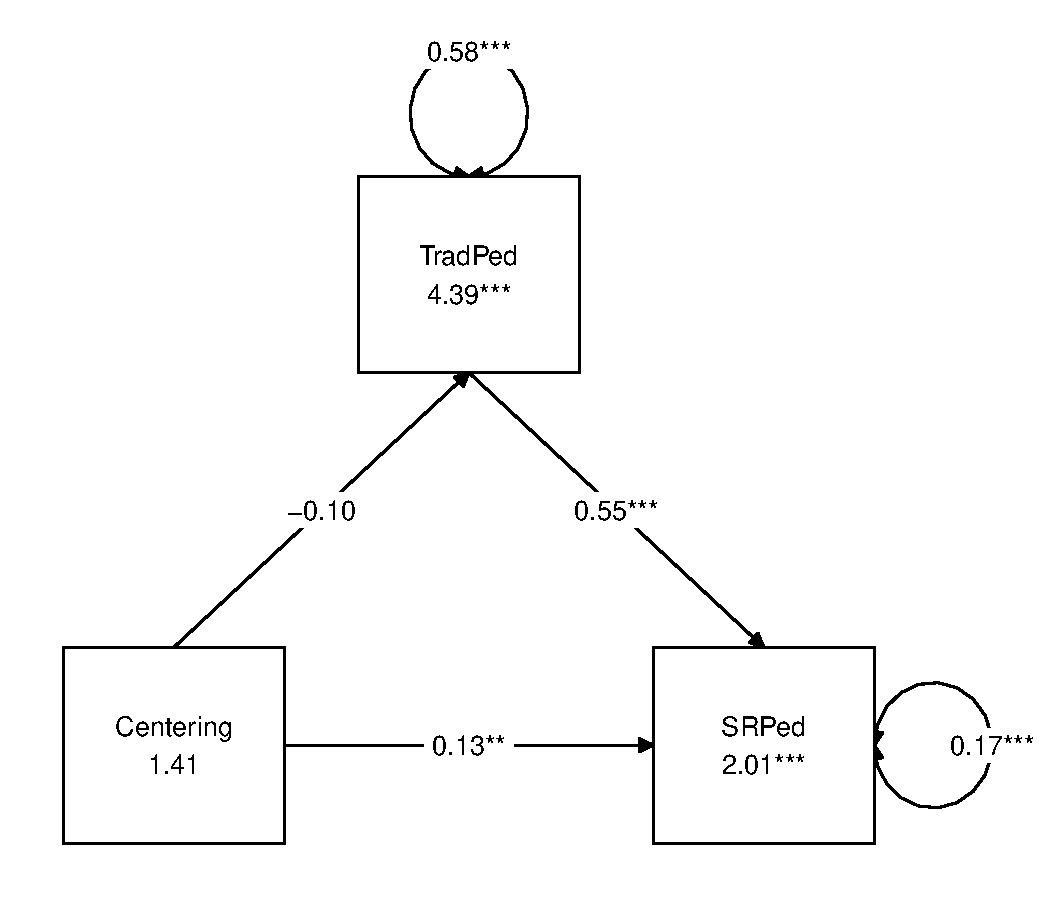
\includegraphics{03-DataDx_files/figure-latex/unnamed-chunk-43-1.pdf}

\begin{Shaded}
\begin{Highlighting}[]
\NormalTok{mice\_ScaleLvl}
\end{Highlighting}
\end{Shaded}

\begin{verbatim}
   StatsPkg Centering TradPed SRPed  
81        1         1       1     1 0
2         1         1       1     0 1
          0         0       0     2 2
\end{verbatim}

There are \emph{2} rows of data because there are only \emph{2} patterns of missingness. The most common pattern is non-missing data (\emph{n} = 81). Two cases are missing the SRPed variable. If our statistical choice uses listwise deletion (i.e., the case is eliminated if one or more variables in the model has missing data), our sample size will be 79. As we will earn in later chapters, there are alternatives (i.e., specifying a FIML option in analyses that use maximum likelihood estimators) that can use all of the cases -- even those with missing data.

\hypertarget{represent-your-work-in-an-apa-style-write-up-added-to-the-writeup-in-the-previous-chapter}{%
\subsubsection*{Represent your work in an APA-style write-up (added to the writeup in the previous chapter}\label{represent-your-work-in-an-apa-style-write-up-added-to-the-writeup-in-the-previous-chapter}}


\begin{quote}
\begin{quote}
Available item analysis (AIA; \citep{parent_handling_2013}) is a strategy for managing missing data that uses available data for analysis and excludes cases with missing data points only for analyses in which the data points would be directly involved. Parent (2013) suggested that AIA is equivalent to more complex methods (e.g., multiple imputation) across a number of variations of sample size, magnitude of associations among items, and degree of missingness. Thus, we utilized Parent's recommendations to guide our approach to managing missing data. Missing data analyses were conducted with tools in base R as well as the R packages, \emph{psych} (v. 2.3.6) and \emph{mice} (v. 3.16.0).
\end{quote}
\end{quote}

\begin{quote}
\begin{quote}
Across cases that were deemed eligible on the basis of the inclusion/exclusion criteria, missingness ranged from 0 to 100\%. Across the dataset, 3.86\% of cells had missing data and 87.88\% of cases had nonmissing data.
\end{quote}
\end{quote}

\begin{quote}
\begin{quote}
Across the 84 cases for which the scoring protocol was applied, missingness ranged from 0 to 67\%. After eliminating cases with greater than 20\% missing, the dataset analyzed included 83 cases. In this dataset we had less than 1\% (0.60\%) missing across the df; 98\% of the rows had nonmissing data.
\end{quote}
\end{quote}

\hypertarget{data-dx}{%
\subsection{Data Dx}\label{data-dx}}

\hypertarget{calculate-alpha-coefficients-for-scalessubscales}{%
\subsubsection*{Calculate alpha coefficients for scales/subscales}\label{calculate-alpha-coefficients-for-scalessubscales}}


To calculate the alpha coefficients, we need item-level data. We will return to \emph{scrub\_df} that contains the item-level data.

\begin{Shaded}
\begin{Highlighting}[]
\CommentTok{\# alpha for the traditional pedagogy scale}
\NormalTok{psych}\SpecialCharTok{::}\FunctionTok{alpha}\NormalTok{(scrub\_df[}\FunctionTok{c}\NormalTok{(}\StringTok{"ClearResponsibilities"}\NormalTok{, }\StringTok{"EffectiveAnswers"}\NormalTok{, }\StringTok{"Feedback"}\NormalTok{,}
    \StringTok{"ClearOrganization"}\NormalTok{, }\StringTok{"ClearPresentation"}\NormalTok{)])}
\end{Highlighting}
\end{Shaded}

\begin{verbatim}

Reliability analysis   
Call: psych::alpha(x = scrub_df[c("ClearResponsibilities", "EffectiveAnswers", 
    "Feedback", "ClearOrganization", "ClearPresentation")])

  raw_alpha std.alpha G6(smc) average_r S/N   ase mean   sd median_r
      0.87      0.88    0.87      0.59 7.2 0.022  4.3 0.72     0.58

    95% confidence boundaries 
         lower alpha upper
Feldt     0.83  0.87  0.91
Duhachek  0.83  0.87  0.92

 Reliability if an item is dropped:
                      raw_alpha std.alpha G6(smc) average_r S/N alpha se  var.r
ClearResponsibilities      0.84      0.84    0.82      0.57 5.3    0.029 0.0110
EffectiveAnswers           0.84      0.84    0.81      0.57 5.2    0.029 0.0088
Feedback                   0.87      0.87    0.86      0.64 7.0    0.023 0.0053
ClearOrganization          0.86      0.86    0.83      0.60 6.1    0.025 0.0067
ClearPresentation          0.83      0.84    0.81      0.57 5.3    0.030 0.0074
                      med.r
ClearResponsibilities  0.55
EffectiveAnswers       0.58
Feedback               0.63
ClearOrganization      0.59
ClearPresentation      0.57

 Item statistics 
                       n raw.r std.r r.cor r.drop mean   sd
ClearResponsibilities 83  0.85  0.85  0.80   0.74  4.5 0.87
EffectiveAnswers      84  0.84  0.85  0.82   0.76  4.4 0.79
Feedback              82  0.74  0.75  0.65   0.60  4.3 0.81
ClearOrganization     84  0.82  0.80  0.74   0.68  4.1 1.04
ClearPresentation     84  0.85  0.85  0.81   0.76  4.2 0.87

Non missing response frequency for each item
                         1    2    3    4    5 miss
ClearResponsibilities 0.01 0.05 0.04 0.27 0.64 0.01
EffectiveAnswers      0.02 0.00 0.05 0.40 0.52 0.00
Feedback              0.01 0.01 0.11 0.38 0.49 0.02
ClearOrganization     0.04 0.07 0.07 0.43 0.39 0.00
ClearPresentation     0.01 0.06 0.04 0.46 0.43 0.00
\end{verbatim}

\begin{quote}
\begin{quote}
Cronbach's alpha for the traditional pedagogy scale was 0.88.
\end{quote}
\end{quote}

\begin{Shaded}
\begin{Highlighting}[]
\CommentTok{\# alpha for the traditional pedagogy scale}
\NormalTok{psych}\SpecialCharTok{::}\FunctionTok{alpha}\NormalTok{(scrub\_df[}\FunctionTok{c}\NormalTok{(}\StringTok{"InclusvClassrm"}\NormalTok{, }\StringTok{"EquitableEval"}\NormalTok{, }\StringTok{"DEIintegration"}\NormalTok{,}
    \StringTok{"DEIintegration"}\NormalTok{)])}
\end{Highlighting}
\end{Shaded}

\begin{verbatim}
Warning in cor.smooth(r): Matrix was not positive definite, smoothing was done
\end{verbatim}

\begin{verbatim}
In smc, smcs < 0 were set to .0
In smc, smcs < 0 were set to .0
In smc, smcs < 0 were set to .0
In smc, smcs < 0 were set to .0
\end{verbatim}

\begin{verbatim}

Reliability analysis   
Call: psych::alpha(x = scrub_df[c("InclusvClassrm", "EquitableEval", 
    "DEIintegration", "DEIintegration")])

  raw_alpha std.alpha G6(smc) average_r S/N   ase mean   sd median_r
      0.85      0.85     0.7      0.58 5.6 0.025  4.5 0.62     0.55

    95% confidence boundaries 
         lower alpha upper
Feldt     0.79  0.85   0.9
Duhachek  0.80  0.85   0.9

 Reliability if an item is dropped:
                 raw_alpha std.alpha G6(smc) average_r S/N alpha se  var.r
InclusvClassrm        0.84      0.83    0.58      0.61 4.8    0.027 0.1115
EquitableEval         0.88      0.88    0.63      0.71 7.3    0.025 0.0640
DEIintegration        0.74      0.75    0.68      0.50 3.1    0.046 0.0054
DEIintegration.1      0.74      0.75    0.68      0.50 3.1    0.046 0.0054
                 med.r
InclusvClassrm    0.42
EquitableEval     0.56
DEIintegration    0.53
DEIintegration.1  0.53

 Item statistics 
                  n raw.r std.r r.cor r.drop mean   sd
InclusvClassrm   80  0.85  0.80  0.75   0.62  4.6 0.72
EquitableEval    84  0.71  0.72  0.60   0.51  4.7 0.50
DEIintegration   70  0.96  0.90  0.71   0.85  4.5 0.79
DEIintegration.1 70  0.96  0.90  0.71   0.85  4.5 0.79

Non missing response frequency for each item
                    1    3    4    5 miss
InclusvClassrm   0.01 0.06 0.21 0.71 0.05
EquitableEval    0.00 0.01 0.32 0.67 0.00
DEIintegration   0.00 0.19 0.17 0.64 0.17
DEIintegration.1 0.00 0.19 0.17 0.64 0.17
\end{verbatim}

\begin{quote}
\begin{quote}
Cronbach's alpha for the socially responsive pedagogy scale was 0.85.
\end{quote}
\end{quote}

Both of these are above the recommended value of 0.80.

\hypertarget{evaluate-univariate-normality-skew-kurtosis-shapiro-wilks}{%
\subsubsection*{Evaluate univariate normality (skew, kurtosis, Shapiro-Wilks)}\label{evaluate-univariate-normality-skew-kurtosis-shapiro-wilks}}


We can inspect univariate normality by examining the skew and kurtosis values of the continuously scored variables.

\begin{Shaded}
\begin{Highlighting}[]
\NormalTok{psych}\SpecialCharTok{::}\FunctionTok{describe}\NormalTok{(scored, }\AttributeTok{type =} \DecValTok{1}\NormalTok{)}
\end{Highlighting}
\end{Shaded}

\begin{verbatim}
           vars  n mean   sd median trimmed  mad  min max range  skew kurtosis
StatsPkg*     1 83 1.73 0.44   2.00    1.79 0.00 1.00   2  1.00 -1.06    -0.87
Centering*    2 83 1.36 0.48   1.00    1.33 0.00 1.00   2  1.00  0.58    -1.67
TradPed       3 83 4.29 0.72   4.40    4.40 0.59 1.20   5  3.80 -1.75     4.49
SRPed         4 81 4.51 0.58   4.75    4.60 0.37 2.33   5  2.67 -1.19     1.30
             se
StatsPkg*  0.05
Centering* 0.05
TradPed    0.08
SRPed      0.06
\end{verbatim}

When we use the ``type=1'' argument, the skew and kurtosis indices in the \emph{psych} package can be interpreted according to Kline's \citeyearpar{kline_data_2016} guidelines.

\begin{quote}
\begin{quote}
Regarding the distributional characteristics of the data, skew and kurtosis values for our continuously scaled variables fall below the thresholds of concern (i.e., absolute value of 3 for skew; absolute value of 10 for kurtosis) identified by Kline \citeyearpar{kline_data_2016}.
\end{quote}
\end{quote}

Still at the univariate level, we can apply the Shapiro-Wilk test of normality to each of our continuously scaled variables. When the \(p\) value is \textless{} .05, the variable's distribution is deviates from a normal distribution to a degree that is statistically significant. Below, the plotting of the histogram with a normal curve superimposed shows how the distribution approximates one that is normal.

\begin{Shaded}
\begin{Highlighting}[]
\CommentTok{\# The shapiro{-}test is in base R; it\textquotesingle{}s specification is simple:}
\CommentTok{\# shapiro.test(df$variable) I added the object (and had to list it}
\CommentTok{\# below) so I can use the inline text function}
\FunctionTok{shapiro.test}\NormalTok{(scored}\SpecialCharTok{$}\NormalTok{TradPed)}
\end{Highlighting}
\end{Shaded}

\begin{verbatim}

    Shapiro-Wilk normality test

data:  scored$TradPed
W = 0.83046, p-value = 0.0000000245
\end{verbatim}

\begin{Shaded}
\begin{Highlighting}[]
\FunctionTok{shapiro.test}\NormalTok{(scored}\SpecialCharTok{$}\NormalTok{SRPed)}
\end{Highlighting}
\end{Shaded}

\begin{verbatim}

    Shapiro-Wilk normality test

data:  scored$SRPed
W = 0.81782, p-value = 0.0000000134
\end{verbatim}

Both variable differ from a normal distribution in a statistically significant way.

\begin{itemize}
\tightlist
\item
  For the traditional pedagogy variable, \(W = 0.830, p < 0.001\)
\item
  for the socially responsive pedagogy variable, \(0.818, p < 0.001\)
\end{itemize}

Obtaining a quick \emph{psych::pairs.panel} can provide a quick glimpse of the distribution.

\begin{Shaded}
\begin{Highlighting}[]
\NormalTok{psych}\SpecialCharTok{::}\FunctionTok{pairs.panels}\NormalTok{(scored, }\AttributeTok{stars =} \ConstantTok{TRUE}\NormalTok{, }\AttributeTok{lm =} \ConstantTok{TRUE}\NormalTok{)}
\end{Highlighting}
\end{Shaded}

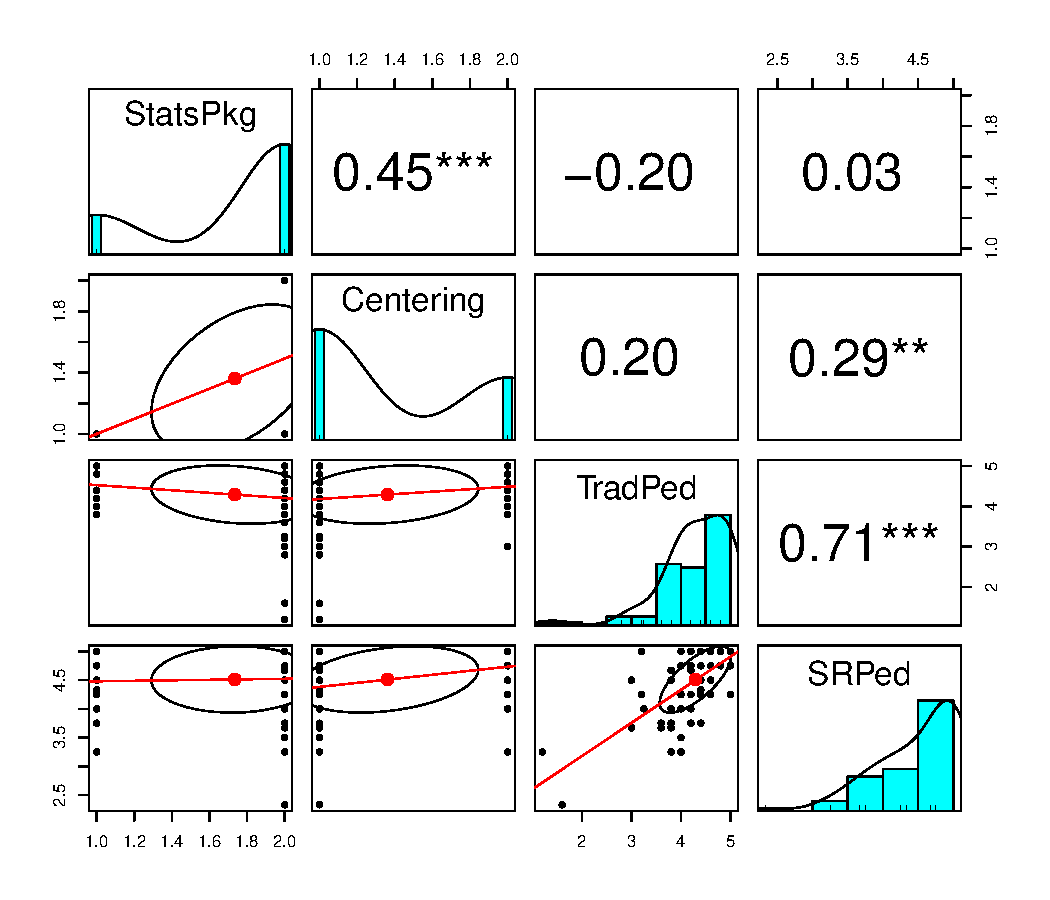
\includegraphics{03-DataDx_files/figure-latex/unnamed-chunk-48-1.pdf}

CUMULATIVE CAPTURE FOR THE APA STYLE WRITE-UP:

\begin{quote}
\begin{quote}
Regarding the distributional characteristics of the data, skew and kurtosis values of the variables fell below the values of 3 (skew) and 10 (kurtosis) that Kline suggests are concerning \citeyearpar{kline_principles_2016}. Results of the Shapiro-Wilk test of normality indicate that our variables assessing the traditional pedagogy (\(W = 0.830, p < 0.001\)) and socially responsive pedagogy (0.818, p \textless{} 0.001) are statistically significantly different than a normal distribution. Inspection of distributions of the variables indicated that both course evaluation variables were negatively skewed, with a large proportion of high scores.
\end{quote}
\end{quote}

\hypertarget{evaluate-multivarite-normality-mahalanobis-test}{%
\subsubsection*{Evaluate multivarite normality (Mahalanobis test)}\label{evaluate-multivarite-normality-mahalanobis-test}}


In more complex models, multivariate normality is probably a more useful analysis. Although I am teaching this evaluation in advance of the formal analysis, as demonstrated in many of \href{https://lhbikos.github.io/ReCenterPsychStats/analysis-of-variance.html}{ReCentering Psych Stats ANOVA chapters}, this can also be assessed by examining the distribution of residuals after the analysis is complete.

Multivariate normality can be assessed with the continuously scaled variables. The code below includes the only two continuously scaled variables. The code simultaneously (a) appends the df with a Mahalanobis value and (b) creates a QQ plot. Dots that stray from the line are the scores that are contributing to multivariate non-normality.

\begin{Shaded}
\begin{Highlighting}[]
\NormalTok{scored}\SpecialCharTok{$}\NormalTok{Mahal }\OtherTok{\textless{}{-}}\NormalTok{ psych}\SpecialCharTok{::}\FunctionTok{outlier}\NormalTok{(scored[}\FunctionTok{c}\NormalTok{(}\StringTok{"TradPed"}\NormalTok{, }\StringTok{"SRPed"}\NormalTok{)])}
\end{Highlighting}
\end{Shaded}

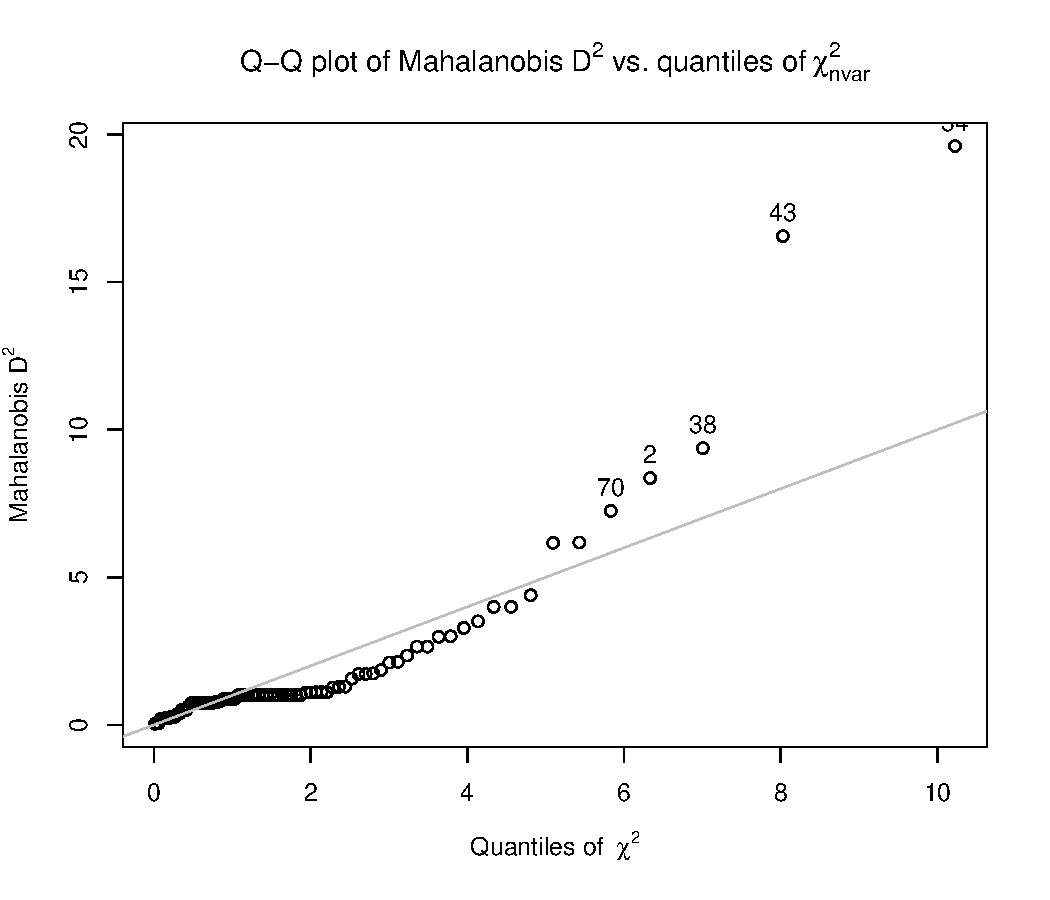
\includegraphics{03-DataDx_files/figure-latex/unnamed-chunk-49-1.pdf}

We can analyze the distributional characteristics of the Mahalanobis values with \emph{psych::describe}. It is possible, then to analyze the Mahalanobis distance values.

\begin{Shaded}
\begin{Highlighting}[]
\NormalTok{psych}\SpecialCharTok{::}\FunctionTok{describe}\NormalTok{(scored}\SpecialCharTok{$}\NormalTok{Mahal)}
\end{Highlighting}
\end{Shaded}

\begin{verbatim}
   vars  n mean   sd median trimmed  mad  min   max range skew kurtosis   se
X1    1 83 1.97 3.12   1.01    1.27 0.42 0.03 19.61 19.58 3.75    15.87 0.34
\end{verbatim}

Using this information we can determine cases that have a Mahalanobis distance values that exceeds three standard deviations around the median. In fact, we can have these noted in a column in the dataframe.

\begin{Shaded}
\begin{Highlighting}[]
\CommentTok{\# creates a variable indicating TRUE or FALSE if an item is an}
\CommentTok{\# outlier}
\NormalTok{scored}\SpecialCharTok{$}\NormalTok{MOutlier }\OtherTok{\textless{}{-}}\NormalTok{ dplyr}\SpecialCharTok{::}\FunctionTok{if\_else}\NormalTok{(scored}\SpecialCharTok{$}\NormalTok{Mahal }\SpecialCharTok{\textgreater{}}\NormalTok{ (}\FunctionTok{median}\NormalTok{(scored}\SpecialCharTok{$}\NormalTok{Mahal) }\SpecialCharTok{+}
\NormalTok{    (}\DecValTok{3} \SpecialCharTok{*} \FunctionTok{sd}\NormalTok{(scored}\SpecialCharTok{$}\NormalTok{Mahal))), }\ConstantTok{TRUE}\NormalTok{, }\ConstantTok{FALSE}\NormalTok{)}

\CommentTok{\# shows us the first 6 rows of the data so we can see the new}
\CommentTok{\# variables (Mahal, MOutlier)}
\FunctionTok{head}\NormalTok{(scored)}
\end{Highlighting}
\end{Shaded}

\begin{verbatim}
  StatsPkg Centering TradPed SRPed     Mahal MOutlier
1     SPSS       Pre     4.2    NA 0.0319020    FALSE
2        R       Pre     2.8    NA 8.3615550    FALSE
3        R        Re     3.8   4.5 0.8702516    FALSE
4        R        Re     5.0   5.0 1.0087776    FALSE
5        R        Re     4.8   5.0 0.7363631    FALSE
6        R        Re     4.0   5.0 2.6509906    FALSE
\end{verbatim}

\begin{Shaded}
\begin{Highlighting}[]
\FunctionTok{library}\NormalTok{(tidyverse)}
\CommentTok{\# counts frequency TRUE and FALSE indicating outlier or not}
\NormalTok{OutlierCount }\OtherTok{\textless{}{-}}\NormalTok{ scored }\SpecialCharTok{\%\textgreater{}\%}
\NormalTok{    dplyr}\SpecialCharTok{::}\FunctionTok{count}\NormalTok{(MOutlier)}

\CommentTok{\# calculating how many outliers a slightly different way}
\FunctionTok{nrow}\NormalTok{(scored) }\SpecialCharTok{{-}}\NormalTok{ OutlierCount}
\end{Highlighting}
\end{Shaded}

\begin{verbatim}
  MOutlier  n
1       83  2
2       82 81
\end{verbatim}

When we identify outliers we often ask if we should delete them or transform the data. A general rule of thumb is to look for ``jumps'' in the Mahalanobis distance values. If they are progressing steadily and there is no ``jump,'' researchers will often retain the outliers.

In this case, I do see a jump. When I sort the df on Mahal values, the jump from 9.37 to 16.56 is much different than the more gradual increase in values that precedes it. Therefore, I think I will delete cases with Mahalanobis values greater than 10 (a number I ``just picked'').

\begin{Shaded}
\begin{Highlighting}[]
\NormalTok{scored }\OtherTok{\textless{}{-}}\NormalTok{ dplyr}\SpecialCharTok{::}\FunctionTok{filter}\NormalTok{(scored, Mahal }\SpecialCharTok{\textless{}} \StringTok{"10"}\NormalTok{)}
\end{Highlighting}
\end{Shaded}

\begin{quote}
\begin{quote}
We evaluated multivariate normality with the Mahalanobis distance test. Specifically, we used the \emph{psych::outlier()} function and included both continuous variables in the calculation. Our visual inspection of the Q-Q plot suggested that the plotted line strayed from the straight line as the quantiles increased. Additionally, we appended the Mahalanobis distance scores as a variable to the data. Analyzing this variable, we found that 2 cases exceed three standard deviations beyond the median. Because there was a substantial ``jump'' between the non-outliers and these two variables we chose to delete them.
\end{quote}
\end{quote}

\hypertarget{represent-your-work-in-an-apa-style-write-up-added-to-the-writeup-in-the-previous-chapter-1}{%
\subsubsection*{Represent your work in an APA-style write-up (added to the writeup in the previous chapter)}\label{represent-your-work-in-an-apa-style-write-up-added-to-the-writeup-in-the-previous-chapter-1}}


\begin{quote}
\begin{quote}
This is a secondary analysis of data involved in a more comprehensive dataset that included students taking multiple statistics courses (\emph{N} = 310). Having retrieved this data from a repository in the Open Science Framework, only those who consented to participation in the study were included. Data used in these analyses were 84 students who completed the multivariate clas.
\end{quote}
\end{quote}

\begin{quote}
\begin{quote}
Available item analysis (AIA; \citep{parent_handling_2013}) is a strategy for managing missing data that uses available data for analysis and excludes cases with missing data points only for analyses in which the data points would be directly involved. Parent (2013) suggested that AIA is equivalent to more complex methods (e.g., multiple imputation) across a number of variations of sample size, magnitude of associations among items, and degree of missingness. Thus, we utilized Parent's recommendations to guide our approach to managing missing data. Missing data analyses were conducted with tools in base R as well as the R packages, \emph{psych} (v. 2.3.6) and \emph{mice} (v. 3.16.0).
\end{quote}
\end{quote}

\begin{quote}
\begin{quote}
Across cases that were deemed eligible on the basis of the inclusion/exclusion criteria, missingness ranged from 0 to 100\%. Across the dataset, 3.86\% of cells had missing data and 87.88\% of cases had nonmissing data.
\end{quote}
\end{quote}

\begin{quote}
\begin{quote}
Across the 84 cases for which the scoring protocol was applied, missingness ranged from 0 to 67\%. After eliminating cases with greater than 20\% missing, the dataset analyzed included 83 cases. In this dataset we had less than 1\% (0.60\%) missing across the df; 98\% of the rows had nonmissing data.
\end{quote}
\end{quote}

\begin{quote}
\begin{quote}
Regarding the distributional characteristics of the data, skew and kurtosis values of the variables fell below the values of 3 (skew) and 10 (kurtosis) that Kline suggests are concerning \citeyearpar{kline_principles_2016}. Results of the Shapiro-Wilk test of normality indicate that our variables assessing the traditional pedagogy (\(W = 0.830, p < 0.001\)) and socially responsive pedagogy (0.818, p \textless{} 0.001) are statistically significantly different than a normal distribution. Inspection of distributions of the variables indicated that both course evaluation variables were negatively skewed, with a large proportion of high scores.
\end{quote}
\end{quote}

\begin{quote}
\begin{quote}
We evaluated multivariate normality with the Mahalanobis distance test. Specifically, we used the \emph{psych::outlier()} function and included both continuous variables in the calculation. Our visual inspection of the Q-Q plot suggested that the plotted line strayed from the straight line as the quantiles increased. Additionally, we appended the Mahalanobis distance scores as a variable to the data. Analyzing this variable, we found that 2 cases exceed three standard deviations beyond the median. Because there was a substantial ``jump'' between the non-outliers and these two variables we chose to delete them.
\end{quote}
\end{quote}

\hypertarget{conduct-a-quick-analysis-e.g.-regression-anova-including-at-least-three-variables}{%
\subsubsection*{Conduct a quick analysis (e.g., regression, ANOVA) including at least three variables}\label{conduct-a-quick-analysis-e.g.-regression-anova-including-at-least-three-variables}}


\begin{Shaded}
\begin{Highlighting}[]
\NormalTok{SRPed\_fit }\OtherTok{\textless{}{-}} \FunctionTok{lm}\NormalTok{(SRPed }\SpecialCharTok{\textasciitilde{}}\NormalTok{ StatsPkg }\SpecialCharTok{+}\NormalTok{ Centering }\SpecialCharTok{+}\NormalTok{ TradPed, }\AttributeTok{data =}\NormalTok{ scored)}
\FunctionTok{summary}\NormalTok{(SRPed\_fit)}
\end{Highlighting}
\end{Shaded}

\begin{verbatim}

Call:
lm(formula = SRPed ~ StatsPkg + Centering + TradPed, data = scored)

Residuals:
     Min       1Q   Median       3Q      Max 
-0.56099 -0.14406  0.01551  0.10594  0.46498 

Coefficients:
            Estimate Std. Error t value          Pr(>|t|)    
(Intercept)  1.46330    0.34441   4.249 0.000077464849487 ***
StatsPkgR    0.13251    0.08056   1.645             0.105    
CenteringRe  0.05666    0.07423   0.763             0.448    
TradPed      0.68663    0.07365   9.323 0.000000000000332 ***
---
Signif. codes:  0 '***' 0.001 '**' 0.01 '*' 0.05 '.' 0.1 ' ' 1

Residual standard error: 0.2433 on 59 degrees of freedom
  (1 observation deleted due to missingness)
Multiple R-squared:  0.6167,    Adjusted R-squared:  0.5972 
F-statistic: 31.64 on 3 and 59 DF,  p-value: 0.000000000002547
\end{verbatim}

\hypertarget{results-2}{%
\subsection{Results}\label{results-2}}

\begin{quote}
\begin{quote}
Results of a multiple regression predicting the socially responsive course evaluation ratings indicated that neither the transition from SPSS to R (\(B = 0.133, p = 0.105\)) nor the transition to an explicitly recentered curriculum (\(B = 0.057, p = 0.448) led to statistically significant diferences. In contrast, traditional pedagogy had a strong, positive effect on evaluations of socially responsive pedagogy (\)B = 0.686, p \textless{} 0.001). The model accounted for 62\% of the variance and was statistically significant (\(p , 0.001\)). Means, standard deviations, and correlations among variables are presented in Table 1; results of the regression model are presented in Table 2.
\end{quote}
\end{quote}

\begin{Shaded}
\begin{Highlighting}[]
\NormalTok{apaTables}\SpecialCharTok{::}\FunctionTok{apa.cor.table}\NormalTok{(scored[}\FunctionTok{c}\NormalTok{(}\StringTok{"SRPed"}\NormalTok{, }\StringTok{"StatsPkg"}\NormalTok{, }\StringTok{"Centering"}\NormalTok{, }\StringTok{"TradPed"}\NormalTok{)],}
    \AttributeTok{table.number =} \DecValTok{1}\NormalTok{, }\AttributeTok{show.sig.stars =} \ConstantTok{TRUE}\NormalTok{, }\AttributeTok{filename =} \StringTok{"Table1\_\_DataDx\_HW.doc"}\NormalTok{)}
\end{Highlighting}
\end{Shaded}

\begin{verbatim}


Table 1 

Means, standard deviations, and correlations with confidence intervals
 

  Variable   M    SD   1         
  1. SRPed   4.69 0.38           
                                 
  2. TradPed 4.53 0.43 .76**     
                       [.63, .85]
                                 

Note. M and SD are used to represent mean and standard deviation, respectively.
Values in square brackets indicate the 95% confidence interval.
The confidence interval is a plausible range of population correlations 
that could have caused the sample correlation (Cumming, 2014).
 * indicates p < .05. ** indicates p < .01.
 
\end{verbatim}

\begin{Shaded}
\begin{Highlighting}[]
\NormalTok{apaTables}\SpecialCharTok{::}\FunctionTok{apa.reg.table}\NormalTok{(SRPed\_fit, }\AttributeTok{table.number =} \DecValTok{2}\NormalTok{, }\AttributeTok{filename =} \StringTok{"SRPed\_table.doc"}\NormalTok{)}
\end{Highlighting}
\end{Shaded}

\begin{verbatim}


Table 2 

Regression results using SRPed as the criterion
 

   Predictor      b      b_95%_CI sr2  sr2_95%_CI             Fit
 (Intercept) 1.46**  [0.77, 2.15]                                
   StatsPkgR   0.13 [-0.03, 0.29] .02 [-.02, .06]                
 CenteringRe   0.06 [-0.09, 0.21] .00 [-.02, .02]                
     TradPed 0.69**  [0.54, 0.83] .56  [.40, .73]                
                                                      R2 = .617**
                                                  95% CI[.43,.70]
                                                                 

Note. A significant b-weight indicates the semi-partial correlation is also significant.
b represents unstandardized regression weights. 
sr2 represents the semi-partial correlation squared.
Square brackets are used to enclose the lower and upper limits of a confidence interval.
* indicates p < .05. ** indicates p < .01.
 
\end{verbatim}

\hypertarget{multimp}{%
\chapter{Multiple Imputation (A Brief Demo)}\label{multimp}}

\href{https://spu.hosted.panopto.com/Panopto/Pages/Viewer.aspx?pid=94d59efe-3f02-4c65-b068-ad01003e09a9}{Screencasted Lecture Link}

Multiple imputation is a tool for managing missing data that works with the whole raw data file to impute values for missing data for \emph{multiple sets} (e.g., 5-20) of the raw data. Those multiple sets are considered together in analyses (such as regression) and interpretation is made on the pooled results. Much has been written about multiple imputation and, if used, should be done with many considerations. This chapter is intended as a brief introduction. In this chapter, I demonstrate the use of multiple imputation with the data from the \href{https://spupsych.az1.qualtrics.com/jfe/form/SV_b2cClqAlLGQ6nLU}{Rate-a-Recent-Course: A ReCentering Psych Stats Exercise} that has served as the research vignette for the first few chapters of this OER.

\hypertarget{navigating-this-lesson-3}{%
\section{Navigating this Lesson}\label{navigating-this-lesson-3}}

There is about one hour of lecture. If you work through the materials with me it would be good to add another hour (to an hour-and-a-half).

While the majority of R objects and data you will need are created within the R script that sources the chapter, there are a few that cannot be created from within the R framework. Additionally, sometimes links fail. All original materials are provided at the \href{https://github.com/lhbikos/ReC_MultivModel}{Github site} that hosts the book. More detailed guidelines for ways to access all these materials are provided in the OER's \protect\hyperlink{ReCintro}{introduction}

\hypertarget{learning-objectives-3}{%
\subsection{Learning Objectives}\label{learning-objectives-3}}

Learning objectives from this lecture include the following:

\begin{itemize}
\tightlist
\item
  Describe circumstances under which multiple imputation would be appropriate
\item
  List and define the stages in multiple imputation.
\item
  Apply multiple imputation to a dataset that has missingness
\item
  Interpret results from a simple regression that uses multiple imputation
\item
  Articulate how multiple imputation fits into the workflow for scrubbing and scoring data.
\item
  Write up the results of an the process of imputation from raw data through analyzing a simple regression (or similar) analysis.
\end{itemize}

\hypertarget{planning-for-practice-3}{%
\subsection{Planning for Practice}\label{planning-for-practice-3}}

The suggestions for practice are a continuation from the three prior chapters. If you have completed one or more of those assignments, you should have worked through the steps in preparing a data set and evaluating its appropriateness for the planned, statistical, analysis. This chapter takes a deviation from the AIA \citep{parent_handling_2013} approach that was the focus of the first few chapters in that we used multiple imputation as the approach for managing missingness. Options, of graded complexity, for practice include:

\begin{itemize}
\tightlist
\item
  Repeating the steps in the chapter with the most recent data from the Rate-A-Recent-Course survey; differences will be in the number of people who have completed the survey since the chapter was written.
\item
  Use the dataset that is the source of the chapter, but score a different set of items that you choose.
\item
  Begin with raw data to which you have access.
\end{itemize}

\hypertarget{readings-resources-3}{%
\subsection{Readings \& Resources}\label{readings-resources-3}}

In preparing this chapter, I drew heavily from the following resource(s). Other resources are cited (when possible, linked) in the text with complete citations in the reference list.

\begin{itemize}
\tightlist
\item
  Enders, C. K. (2017). Multiple imputation as a flexible tool for missing data handling in clinical research. \emph{Behaviour Research and Therapy}, 98, 4--18.

  \begin{itemize}
  \tightlist
  \item
    Craig Enders is a leading expert in the analysis and management of missing data. This article is useful in describing multiple imputation as a method for managing missingness.
  \end{itemize}
\item
  Katitas, A. (2019). Getting Started with Multiple Imputation in R. University of Virginia Library: Research Data Services + Sciences. \url{https://library.virginia.edu/data/articles/getting-started-with-multiple-imputation-in-r}

  \begin{itemize}
  \tightlist
  \item
    Tutorial for conducting multiple imputation in R.
  \end{itemize}
\item
  Kline Ch4, Data Preparation \& Psychometrics Review (pp.~72/Outliers - 88/Modern Methods)
\item
  Kline's chapter is my ``go-to'' for making decisions about preparing data for analysis.
\end{itemize}

\hypertarget{packages-3}{%
\subsection{Packages}\label{packages-3}}

The script below will (a) check to see if the following packages are installed on your computer and, if not (b) install them.

\begin{Shaded}
\begin{Highlighting}[]
\CommentTok{\# will install the package if not already installed}
\ControlFlowTok{if}\NormalTok{ (}\SpecialCharTok{!}\FunctionTok{require}\NormalTok{(qualtRics)) \{}
    \FunctionTok{install.packages}\NormalTok{(}\StringTok{"qualtRics"}\NormalTok{)}
\NormalTok{\}}
\ControlFlowTok{if}\NormalTok{ (}\SpecialCharTok{!}\FunctionTok{require}\NormalTok{(psych)) \{}
    \FunctionTok{install.packages}\NormalTok{(}\StringTok{"psych"}\NormalTok{)}
\NormalTok{\}}
\ControlFlowTok{if}\NormalTok{ (}\SpecialCharTok{!}\FunctionTok{require}\NormalTok{(dplyr)) \{}
    \FunctionTok{install.packages}\NormalTok{(}\StringTok{"dplyr"}\NormalTok{)}
\NormalTok{\}}
\ControlFlowTok{if}\NormalTok{ (}\SpecialCharTok{!}\FunctionTok{require}\NormalTok{(mice)) \{}
    \FunctionTok{install.packages}\NormalTok{(}\StringTok{"mice"}\NormalTok{)}
\NormalTok{\}}
\end{Highlighting}
\end{Shaded}

\hypertarget{workflow-for-multiple-imputation}{%
\section{Workflow for Multiple Imputation}\label{workflow-for-multiple-imputation}}

The following is a proposed workflow for preparing data for analysis.

\begin{figure}
\centering
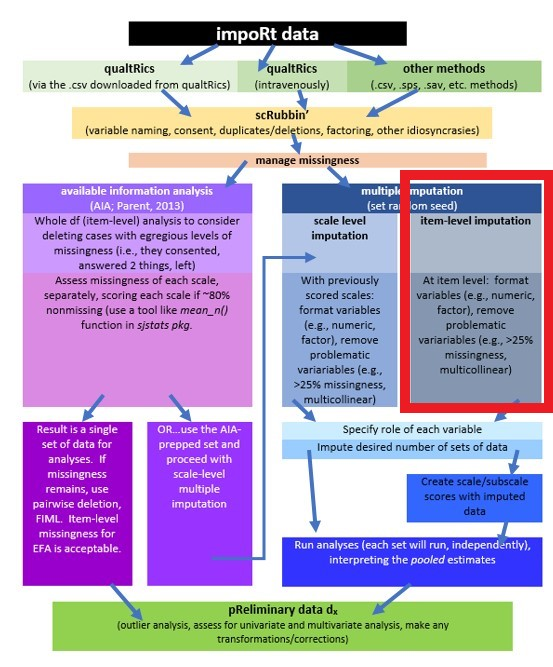
\includegraphics{images/Ch05/scrubscore_mimp_itemlvl.jpg}
\caption{An image of a workflow for scrubbing and scoring data.}
\end{figure}

In this lecture we are working on the right side of the flowchart in the multiple imputation (blue) section. Within it, there are two options, each with a slightly different set of options.

\begin{itemize}
\tightlist
\item
  imputing at the item level

  \begin{itemize}
  \tightlist
  \item
    in this case, scales/subscales are scored after the item-level imputation
  \end{itemize}
\item
  imputating at the scale level

  \begin{itemize}
  \tightlist
  \item
    in this case, scales/subscales are scored prior to the imputation; likely using some of the same criteria as identified in the scoring chapter (i.e., scoring if 75-80\% of data are non-missing). Multiple imputation, then, is used to estimate the remaining, missing values.
  \end{itemize}
\end{itemize}

Whichever approach is used, the imputed variables (multiple sets) are used in a \emph{pooled analysis} and results are interpreted from that analysis.

\hypertarget{research-vignette-3}{%
\section{Research Vignette}\label{research-vignette-3}}

The research vignette comes from the survey titled, \href{https://spupsych.az1.qualtrics.com/jfe/form/SV_b2cClqAlLGQ6nLU}{Rate-a-Recent-Course: A ReCentering Psych Stats Exercise} and is explained in the \protect\hyperlink{scrub}{scrubbing chapter}. In the \protect\hyperlink{score}{scoring chapter} we prepared four variables for analysis. In the \protect\hyperlink{DataDx}{data diagnostics chapter} we assessed the quality of the variables and conducted the multiple regression described below. Details for these are in our \href{./Rate-a-Course_Codebook.pdf}{codebook}.

Let's quickly review the variables in our model:

\begin{itemize}
\tightlist
\item
  Perceived Campus Climate for Black Students includes 6 items, one of which was reverse scored. This scale was adapted from Szymanski et al.'s \citeyearpar{szymanski_perceptions_2020} Campus Climate for LGBTQ students. It has not been evaluated for use with other groups. The Szymanski et al.~analysis suggested that it could be used as a total scale score, or divided into three items each that assess

  \begin{itemize}
  \tightlist
  \item
    College response to LGBTQ students (items 6, 4, 1)
  \item
    LGBTQ stigma (items 3, 2, 5)
  \end{itemize}
\item
  Sense of Belonging includes 3 items. This is a subscale from Bollen and Hoyle's \citeyearpar{bollen_perceived_1990} Perceived Cohesion Scale. There are no items on this scale that require reversing.
\item
  Percent of Black classmates is a single item that asked respondents to estimate the proportion of students in various racial categories
\item
  Percent of BIPOC instructional staff, similarly, asked respondents to identify the racial category of each member of their instructional staff
\end{itemize}

As we noted in the \protect\hyperlink{scrub}{scrubbing chapter}, our design has notable limitations. Briefly, (a) owing to the open source aspect of the data we do not ask about the demographic characteristics of the respondent; (b) the items that ask respondents to \emph{guess} the identities of the instructional staff and to place them in broad categories, (c) we do not provide a ``write-in'' a response. We made these decisions after extensive conversation with stakeholders. The primary reason for these decisions was to prevent potential harm (a) to respondents who could be identified if/when the revealed private information in this open-source survey, and (b) trolls who would write inappropriate or harmful comments.

As I think about ``how these variables go together'' (which is often where I start in planning a study), I suspect parallel mediation. That is the perception of campus climate for Black students would be predicted by the respondent's sense of belonging, mediated in separate paths through the proportion of classmates who are Black and the proportion of BIPOC instructional staff.

\emph{I would like to assess the model by having the instructional staff variable to be the \%Black instructional staff. At the time that this lecture is being prepared, there is not sufficient Black representation in the instructional staff to model this.}

\begin{figure}
\centering
\includegraphics{images/Ch04/BlStuMed.jpg}
\caption{An image of the statistical model for which we are preparing data.}
\end{figure}

As in the \protect\hyperlink{DataDx}{data diagnostic chapter}, I will conclude this chapter by conducting a statistical analysis with the multiply imputed data. Because parallel mediation can be complicated (I teach it in a later chapter), I will demonstrate use of our prepared variables with a simple multiple regression.

\begin{figure}
\centering
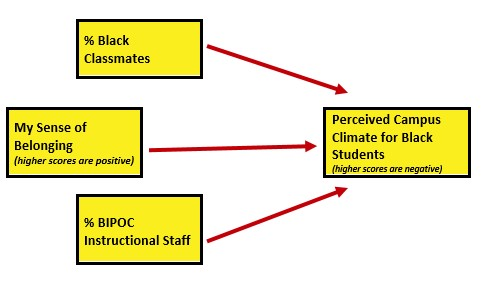
\includegraphics{images/Ch04/BlStuRegression.jpg}
\caption{An image of the statistical model for which we are preparing data.}
\end{figure}

\hypertarget{multiple-imputation-a-super-brief-review}{%
\section{Multiple Imputation -- a Super Brief Review}\label{multiple-imputation-a-super-brief-review}}

Multiple imputation is complex. Numerous quantitative psychologists had critiqued it and provided numerous cautions and guidelines for its use \citep{enders_applied_2010, enders_multiple_2017, little_missing_2008, little_statistical_2002}. In brief,

\hypertarget{steps-in-multiple-imputation}{%
\subsection{Steps in Multiple Imputation}\label{steps-in-multiple-imputation}}

\begin{itemize}
\tightlist
\item
  Multiple imputation starts with a raw data file.

  \begin{itemize}
  \tightlist
  \item
    Multiple imputation assumes that data are MAR (remember, MCAR is the more prestigious one). This means that researchers assume that missing values can be replaced by predictions derived from the observable portion of the dataset.\\
  \end{itemize}
\item
  Multiple datasets (often 5 to 20) are created where missing values are replaced via a randomized process (so the same missing value {[}item 4 for person A{]} will likely have different values for each dataset).
\item
  The desired analysis is conducted simultaneously/separately for each of the imputed sets (so if you imputed 5 sets and wanted a linear regression, you get 5 linear regressions).\\
\item
  A \emph{pooled analysis} uses the point estimates and the standard errors to provide a single result that represents the analysis.
\end{itemize}

In a web-hosted guide from the University of Virginia Library, Katitas \citeyearpar{katitas_getting_2019} provided a user-friendly review and example of using tools in R in a multiple imputation. Katitas' figure is a useful conceptual tool in understanding how multiple imputation works. \emph{This figure is my recreation of Katitas' original.}

\begin{figure}
\centering
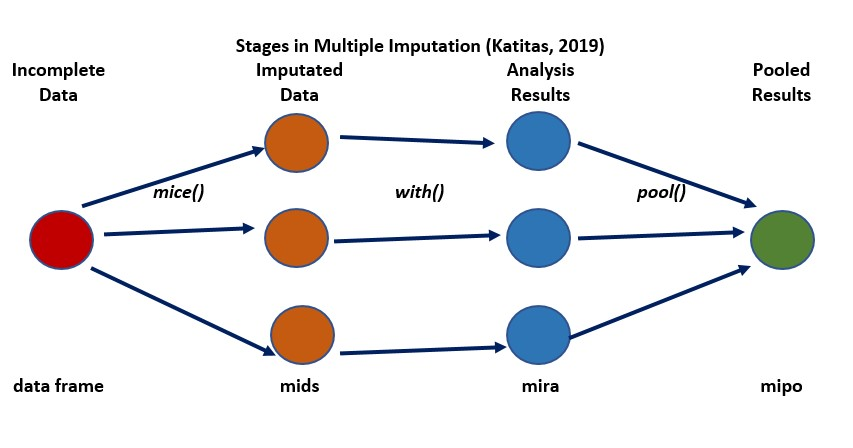
\includegraphics{images/Ch05/KatitasMimpFig.jpg}
\caption{An image adapted from the Katitas multiple imputation guide showing the four stages of multiple imputation.}
\end{figure}

\begin{itemize}
\tightlist
\item
  the dataframe with missing data is the single place we start
\item
  we intervene with a package like \emph{mice()} to
\item
  impute multiple sets of data (filling in the missing variables with different values that are a product of their conditional distribution and an element of ``random'');

  \begin{itemize}
  \tightlist
  \item
    ``mids'' (``multiply imputed dataset'') is an object class where the completed datasets are stored.
  \end{itemize}
\item
  the ``with\_mids'' command allows OLS regression to be run, as many times as we have imputed datasets (in this figure, 3X). It produces different regression coefficients for each datset
\item
  the ``pool'' command pools together the multiple coefficients taking into consideration the value of the coefficients,the standard errors, and the variance of the missing value parameter across the samples.
\end{itemize}

\hypertarget{statistical-approaches-to-multiple-imputation}{%
\subsection{Statistical Approaches to Multiple Imputation}\label{statistical-approaches-to-multiple-imputation}}

\textbf{Joint multivariate normal distribution multiple imputation} assumes that the observed data follow a multivariate normal distribution. The algorithm used draws from this assumed distribution. A drawback is that if the data do not follow a multivariate normal distribution, the imputed values are incorrect. \emph{Amelia} and \emph{norm} packages use this approach.

\textbf{Conditional multiple imputation} is an iterative procedure, modeling the conditional distribution of a certain variable given the other variables. In this way the distribution is assumed for each variable, rather than or the entire dataset. \emph{mice} uses this approach.

\emph{mice}: multivariate imputation by chained equations

\hypertarget{working-the-problem-2}{%
\section{Working the Problem}\label{working-the-problem-2}}

Katitas \citeyearpar{katitas_getting_2019} claims that it is best to impute the data in its rawest form possible because any change would be taking it away from its original distribution. There are debates about how many variables to include in an imputation. Some authors would suggest that researchers include everything that was collected. Others (like me) will trim the dataset to include (a) the variables included in the model, plus (b) auxiliary variables (i.e., variables not in the model, but that are sufficiently non-missing and will provide additional information to the data).

In our case we will want:

Item for the variables represented in our model

\begin{itemize}
\tightlist
\item
  the item level responses to the scales/subscales

  \begin{itemize}
  \tightlist
  \item
    respondents' sense of belonging to campus (3 items)
  \item
    respondents' rating of campus climate for Black students (6 items)
  \end{itemize}
\item
  proportion of BIPOC instructional staff
\item
  proportion of classmates who are Black
\end{itemize}

Auxiliary variables -- let's choose four. One will be the format of the course. Three items will be from the course evaluation.

\begin{itemize}
\tightlist
\item
  format, whether the course was taught in-person, a blend, or virtual
\item
  cEval\_1, ``Course material was presented clearly''
\item
  cEval\_13, ``Where applicable, issues were considered from multiple perspectives''
\item
  cEval\_19, ``My understanding of the subject matter increased over the span of the course''
\end{itemize}

\hypertarget{selecting-and-formatting-variables}{%
\subsection{Selecting and Formatting Variables}\label{selecting-and-formatting-variables}}

There are some guidelines for selecting and formatting variables for imputation.

\begin{itemize}
\tightlist
\item
  Variables should be in their \emph{most natural} state
\item
  Redundant or too highly correlated variables should not be included

  \begin{itemize}
  \tightlist
  \item
    If you reverse coded a variable (we haven't yet), that's ok, but if you have already reverse-coded, then exclude the original variable
  \item
    Redundant variables (or multicollinear variables) may cause the multiple imputation process to cease
  \item
    Violation of this also provides clues for troubleshooting
  \end{itemize}
\item
  Exclude variables with more than 25\% missing
\end{itemize}

To make this as realistic as possible. Let's start with our very raw data. The \protect\hyperlink{scrub}{Scrubbing chapter} provides greater detail on importing data directly from Qualtrics. If you have worked the lessons, consecutively, you know that data can be added to this survey at any time. So that the values in the chapter are consistent, I will use the datafiles that I immediately saved when I conducted the analysis at the time I last updated the chapter.

Please download the .rds or .csv file from \href{https://github.com/lhbikos/ReC_MultivModel}{MultivModel GitHub} site. Please the file in the same folder as your .rmd file. As always, I prefer working with .rds files.

\begin{Shaded}
\begin{Highlighting}[]
\NormalTok{QTRX\_df2 }\OtherTok{\textless{}{-}} \FunctionTok{readRDS}\NormalTok{(}\StringTok{"QTRX\_df230902b.rds"}\NormalTok{)}
\CommentTok{\# QTRX\_df \textless{}{-} read.csv(\textquotesingle{}QTRX\_df230902b.csv\textquotesingle{}, header = TRUE)}
\end{Highlighting}
\end{Shaded}

Next, I apply inclusion/exclusion criteria. As described in the \protect\hyperlink{scrub}{Scrubbing chapter} this includes:

\begin{itemize}
\tightlist
\item
  excluding all \emph{previews}
\item
  including only those who consented
\item
  including only those whose rated course was offered by a U.S. institution
\end{itemize}

\begin{Shaded}
\begin{Highlighting}[]
\FunctionTok{library}\NormalTok{(tidyverse)}
\NormalTok{QTRX\_df2 }\OtherTok{\textless{}{-}}\NormalTok{ dplyr}\SpecialCharTok{::}\FunctionTok{filter}\NormalTok{(QTRX\_df2, DistributionChannel }\SpecialCharTok{!=} \StringTok{"preview"}\NormalTok{)}
\NormalTok{QTRX\_df2 }\OtherTok{\textless{}{-}}\NormalTok{ dplyr}\SpecialCharTok{::}\FunctionTok{filter}\NormalTok{(QTRX\_df2, Consent }\SpecialCharTok{==} \DecValTok{1}\NormalTok{)}
\NormalTok{QTRX\_df2 }\OtherTok{\textless{}{-}}\NormalTok{ dplyr}\SpecialCharTok{::}\FunctionTok{filter}\NormalTok{(QTRX\_df2, USinst }\SpecialCharTok{==} \DecValTok{0}\NormalTok{)}
\end{Highlighting}
\end{Shaded}

Preparing the data also meant renaming some variables that started with numbers (a hassle in R). I also renamed variables on the Campus Climate scale so that we know to which subscale they belong.

\begin{Shaded}
\begin{Highlighting}[]
\CommentTok{\# renaming variables that started with numbers}
\NormalTok{QTRX\_df2 }\OtherTok{\textless{}{-}}\NormalTok{ dplyr}\SpecialCharTok{::}\FunctionTok{rename}\NormalTok{(QTRX\_df2, }\AttributeTok{iRace1 =} \StringTok{"1\_iRace"}\NormalTok{, }\AttributeTok{iRace2 =} \StringTok{"2\_iRace"}\NormalTok{,}
    \AttributeTok{iRace3 =} \StringTok{"3\_iRace"}\NormalTok{, }\AttributeTok{iRace4 =} \StringTok{"4\_iRace"}\NormalTok{, }\AttributeTok{iRace5 =} \StringTok{"5\_iRace"}\NormalTok{, }\AttributeTok{iRace6 =} \StringTok{"6\_iRace"}\NormalTok{,}
    \AttributeTok{iRace7 =} \StringTok{"7\_iRace"}\NormalTok{, }\AttributeTok{iRace8 =} \StringTok{"8\_iRace"}\NormalTok{, }\AttributeTok{iRace9 =} \StringTok{"9\_iRace"}\NormalTok{, }\AttributeTok{iRace10 =} \StringTok{"10\_iRace"}\NormalTok{)}
\CommentTok{\# renaming variables from the identification of classmates}
\NormalTok{QTRX\_df2 }\OtherTok{\textless{}{-}}\NormalTok{ dplyr}\SpecialCharTok{::}\FunctionTok{rename}\NormalTok{(QTRX\_df2, }\AttributeTok{cmBiMulti =}\NormalTok{ Race\_10, }\AttributeTok{cmBlack =}\NormalTok{ Race\_1,}
    \AttributeTok{cmNBPoC =}\NormalTok{ Race\_7, }\AttributeTok{cmWhite =}\NormalTok{ Race\_8, }\AttributeTok{cmUnsure =}\NormalTok{ Race\_2)}
\end{Highlighting}
\end{Shaded}

The Qualtrics download does not include an ID number. Because new variables are always appended to the end of the df, we also include code to make this the first column.

\begin{Shaded}
\begin{Highlighting}[]
\NormalTok{QTRX\_df2 }\OtherTok{\textless{}{-}}\NormalTok{ QTRX\_df2 }\SpecialCharTok{\%\textgreater{}\%}
\NormalTok{    dplyr}\SpecialCharTok{::}\FunctionTok{mutate}\NormalTok{(}\AttributeTok{ID =} \FunctionTok{row\_number}\NormalTok{())}
\CommentTok{\# moving the ID number to the first column; requires}
\NormalTok{QTRX\_df2 }\OtherTok{\textless{}{-}}\NormalTok{ QTRX\_df2 }\SpecialCharTok{\%\textgreater{}\%}
\NormalTok{    dplyr}\SpecialCharTok{::}\FunctionTok{select}\NormalTok{(ID, }\FunctionTok{everything}\NormalTok{())}
\end{Highlighting}
\end{Shaded}

Because this huge df is cumbersome to work with, let's downsize it to be closer to the size we will work with in the imputation

\begin{Shaded}
\begin{Highlighting}[]
\NormalTok{mimp\_df }\OtherTok{\textless{}{-}}\NormalTok{ dplyr}\SpecialCharTok{::}\FunctionTok{select}\NormalTok{(QTRX\_df2, ID, iRace1, iRace2, iRace3, iRace4,}
\NormalTok{    iRace5, iRace6, iRace7, iRace8, iRace9, iRace10, cmBiMulti, cmBlack,}
\NormalTok{    cmNBPoC, cmWhite, cmUnsure, Belong\_1}\SpecialCharTok{:}\NormalTok{Belong\_3, Blst\_1}\SpecialCharTok{:}\NormalTok{Blst\_6, cEval\_1,}
\NormalTok{    cEval\_13, cEval\_19, format)}
\CommentTok{\# glimpse(mimp\_df)}
\FunctionTok{head}\NormalTok{(mimp\_df)}
\end{Highlighting}
\end{Shaded}

\begin{verbatim}
# A tibble: 6 x 29
     ID iRace1 iRace2 iRace3 iRace4 iRace5 iRace6 iRace7 iRace8 iRace9 iRace10
  <int>  <dbl>  <dbl>  <dbl>  <dbl> <lgl>  <lgl>  <lgl>  <lgl>  <lgl>  <lgl>  
1     1      3      1      3     NA NA     NA     NA     NA     NA     NA     
2     2      3     NA     NA     NA NA     NA     NA     NA     NA     NA     
3     3      3      1     NA     NA NA     NA     NA     NA     NA     NA     
4     4      3      1      3     NA NA     NA     NA     NA     NA     NA     
5     5      1     NA     NA     NA NA     NA     NA     NA     NA     NA     
6     6      3     NA     NA     NA NA     NA     NA     NA     NA     NA     
# i 18 more variables: cmBiMulti <dbl>, cmBlack <dbl>, cmNBPoC <dbl>,
#   cmWhite <dbl>, cmUnsure <dbl>, Belong_1 <dbl>, Belong_2 <dbl>,
#   Belong_3 <dbl>, Blst_1 <dbl>, Blst_2 <dbl>, Blst_3 <dbl>, Blst_4 <dbl>,
#   Blst_5 <dbl>, Blst_6 <dbl>, cEval_1 <dbl>, cEval_13 <dbl>, cEval_19 <dbl>,
#   format <dbl>
\end{verbatim}

\hypertarget{creating-composite-variables}{%
\subsection{Creating Composite Variables}\label{creating-composite-variables}}

Qualtrics imports many of the categorical variables as numbers. R often reads them numerically (integers or numbers). If they are directly converted to factors, R will sometimes collapse. In this example, if there is a race that is not represented (e.g., 2 for BiMulti), when the numbers are changed to factors, R will assume it's ordered and will change up the numbers. Therefore, it is ESSENTIAL to check (again and again ad nauseum) to ensure that your variables are recoding in a manner you understand.

\begin{Shaded}
\begin{Highlighting}[]
\NormalTok{mimp\_df}\SpecialCharTok{$}\NormalTok{iRace1 }\OtherTok{=} \FunctionTok{factor}\NormalTok{(mimp\_df}\SpecialCharTok{$}\NormalTok{iRace1, }\AttributeTok{levels =} \FunctionTok{c}\NormalTok{(}\DecValTok{0}\NormalTok{, }\DecValTok{1}\NormalTok{, }\DecValTok{2}\NormalTok{, }\DecValTok{3}\NormalTok{, }\DecValTok{4}\NormalTok{), }\AttributeTok{labels =} \FunctionTok{c}\NormalTok{(}\StringTok{"Black"}\NormalTok{,}
    \StringTok{"nBpoc"}\NormalTok{, }\StringTok{"BiMulti"}\NormalTok{, }\StringTok{"White"}\NormalTok{, }\StringTok{"NotNotice"}\NormalTok{))}
\NormalTok{mimp\_df}\SpecialCharTok{$}\NormalTok{iRace2 }\OtherTok{=} \FunctionTok{factor}\NormalTok{(mimp\_df}\SpecialCharTok{$}\NormalTok{iRace2, }\AttributeTok{levels =} \FunctionTok{c}\NormalTok{(}\DecValTok{0}\NormalTok{, }\DecValTok{1}\NormalTok{, }\DecValTok{2}\NormalTok{, }\DecValTok{3}\NormalTok{, }\DecValTok{4}\NormalTok{), }\AttributeTok{labels =} \FunctionTok{c}\NormalTok{(}\StringTok{"Black"}\NormalTok{,}
    \StringTok{"nBpoc"}\NormalTok{, }\StringTok{"BiMulti"}\NormalTok{, }\StringTok{"White"}\NormalTok{, }\StringTok{"NotNotice"}\NormalTok{))}
\NormalTok{mimp\_df}\SpecialCharTok{$}\NormalTok{iRace3 }\OtherTok{=} \FunctionTok{factor}\NormalTok{(mimp\_df}\SpecialCharTok{$}\NormalTok{iRace3, }\AttributeTok{levels =} \FunctionTok{c}\NormalTok{(}\DecValTok{0}\NormalTok{, }\DecValTok{1}\NormalTok{, }\DecValTok{2}\NormalTok{, }\DecValTok{3}\NormalTok{, }\DecValTok{4}\NormalTok{), }\AttributeTok{labels =} \FunctionTok{c}\NormalTok{(}\StringTok{"Black"}\NormalTok{,}
    \StringTok{"nBpoc"}\NormalTok{, }\StringTok{"BiMulti"}\NormalTok{, }\StringTok{"White"}\NormalTok{, }\StringTok{"NotNotice"}\NormalTok{))}
\NormalTok{mimp\_df}\SpecialCharTok{$}\NormalTok{iRace4 }\OtherTok{=} \FunctionTok{factor}\NormalTok{(mimp\_df}\SpecialCharTok{$}\NormalTok{iRace4, }\AttributeTok{levels =} \FunctionTok{c}\NormalTok{(}\DecValTok{0}\NormalTok{, }\DecValTok{1}\NormalTok{, }\DecValTok{2}\NormalTok{, }\DecValTok{3}\NormalTok{, }\DecValTok{4}\NormalTok{), }\AttributeTok{labels =} \FunctionTok{c}\NormalTok{(}\StringTok{"Black"}\NormalTok{,}
    \StringTok{"nBpoc"}\NormalTok{, }\StringTok{"BiMulti"}\NormalTok{, }\StringTok{"White"}\NormalTok{, }\StringTok{"NotNotice"}\NormalTok{))}
\NormalTok{mimp\_df}\SpecialCharTok{$}\NormalTok{iRace5 }\OtherTok{=} \FunctionTok{factor}\NormalTok{(mimp\_df}\SpecialCharTok{$}\NormalTok{iRace5, }\AttributeTok{levels =} \FunctionTok{c}\NormalTok{(}\DecValTok{0}\NormalTok{, }\DecValTok{1}\NormalTok{, }\DecValTok{2}\NormalTok{, }\DecValTok{3}\NormalTok{, }\DecValTok{4}\NormalTok{), }\AttributeTok{labels =} \FunctionTok{c}\NormalTok{(}\StringTok{"Black"}\NormalTok{,}
    \StringTok{"nBpoc"}\NormalTok{, }\StringTok{"BiMulti"}\NormalTok{, }\StringTok{"White"}\NormalTok{, }\StringTok{"NotNotice"}\NormalTok{))}
\NormalTok{mimp\_df}\SpecialCharTok{$}\NormalTok{iRace6 }\OtherTok{=} \FunctionTok{factor}\NormalTok{(mimp\_df}\SpecialCharTok{$}\NormalTok{iRace6, }\AttributeTok{levels =} \FunctionTok{c}\NormalTok{(}\DecValTok{0}\NormalTok{, }\DecValTok{1}\NormalTok{, }\DecValTok{2}\NormalTok{, }\DecValTok{3}\NormalTok{, }\DecValTok{4}\NormalTok{), }\AttributeTok{labels =} \FunctionTok{c}\NormalTok{(}\StringTok{"Black"}\NormalTok{,}
    \StringTok{"nBpoc"}\NormalTok{, }\StringTok{"BiMulti"}\NormalTok{, }\StringTok{"White"}\NormalTok{, }\StringTok{"NotNotice"}\NormalTok{))}
\NormalTok{mimp\_df}\SpecialCharTok{$}\NormalTok{iRace7 }\OtherTok{=} \FunctionTok{factor}\NormalTok{(mimp\_df}\SpecialCharTok{$}\NormalTok{iRace7, }\AttributeTok{levels =} \FunctionTok{c}\NormalTok{(}\DecValTok{0}\NormalTok{, }\DecValTok{1}\NormalTok{, }\DecValTok{2}\NormalTok{, }\DecValTok{3}\NormalTok{, }\DecValTok{4}\NormalTok{), }\AttributeTok{labels =} \FunctionTok{c}\NormalTok{(}\StringTok{"Black"}\NormalTok{,}
    \StringTok{"nBpoc"}\NormalTok{, }\StringTok{"BiMulti"}\NormalTok{, }\StringTok{"White"}\NormalTok{, }\StringTok{"NotNotice"}\NormalTok{))}
\NormalTok{mimp\_df}\SpecialCharTok{$}\NormalTok{iRace8 }\OtherTok{=} \FunctionTok{factor}\NormalTok{(mimp\_df}\SpecialCharTok{$}\NormalTok{iRace8, }\AttributeTok{levels =} \FunctionTok{c}\NormalTok{(}\DecValTok{0}\NormalTok{, }\DecValTok{1}\NormalTok{, }\DecValTok{2}\NormalTok{, }\DecValTok{3}\NormalTok{, }\DecValTok{4}\NormalTok{), }\AttributeTok{labels =} \FunctionTok{c}\NormalTok{(}\StringTok{"Black"}\NormalTok{,}
    \StringTok{"nBpoc"}\NormalTok{, }\StringTok{"BiMulti"}\NormalTok{, }\StringTok{"White"}\NormalTok{, }\StringTok{"NotNotice"}\NormalTok{))}
\NormalTok{mimp\_df}\SpecialCharTok{$}\NormalTok{iRace9 }\OtherTok{=} \FunctionTok{factor}\NormalTok{(mimp\_df}\SpecialCharTok{$}\NormalTok{iRace9, }\AttributeTok{levels =} \FunctionTok{c}\NormalTok{(}\DecValTok{0}\NormalTok{, }\DecValTok{1}\NormalTok{, }\DecValTok{2}\NormalTok{, }\DecValTok{3}\NormalTok{, }\DecValTok{4}\NormalTok{), }\AttributeTok{labels =} \FunctionTok{c}\NormalTok{(}\StringTok{"Black"}\NormalTok{,}
    \StringTok{"nBpoc"}\NormalTok{, }\StringTok{"BiMulti"}\NormalTok{, }\StringTok{"White"}\NormalTok{, }\StringTok{"NotNotice"}\NormalTok{))}
\NormalTok{mimp\_df}\SpecialCharTok{$}\NormalTok{iRace10 }\OtherTok{=} \FunctionTok{factor}\NormalTok{(mimp\_df}\SpecialCharTok{$}\NormalTok{iRace10, }\AttributeTok{levels =} \FunctionTok{c}\NormalTok{(}\DecValTok{0}\NormalTok{, }\DecValTok{1}\NormalTok{, }\DecValTok{2}\NormalTok{, }\DecValTok{3}\NormalTok{, }\DecValTok{4}\NormalTok{), }\AttributeTok{labels =} \FunctionTok{c}\NormalTok{(}\StringTok{"Black"}\NormalTok{,}
    \StringTok{"nBpoc"}\NormalTok{, }\StringTok{"BiMulti"}\NormalTok{, }\StringTok{"White"}\NormalTok{, }\StringTok{"NotNotice"}\NormalTok{))}
\end{Highlighting}
\end{Shaded}

\begin{Shaded}
\begin{Highlighting}[]
\FunctionTok{head}\NormalTok{(mimp\_df)}
\end{Highlighting}
\end{Shaded}

This is a quick recap of how we calculated the proportion of instructional staff who are BIPOC.

\begin{Shaded}
\begin{Highlighting}[]
\CommentTok{\# creating a count of BIPOC faculty identified by each respondent}
\NormalTok{mimp\_df}\SpecialCharTok{$}\NormalTok{count.BIPOC }\OtherTok{\textless{}{-}} \FunctionTok{apply}\NormalTok{(mimp\_df[}\FunctionTok{c}\NormalTok{(}\StringTok{"iRace1"}\NormalTok{, }\StringTok{"iRace2"}\NormalTok{, }\StringTok{"iRace3"}\NormalTok{, }\StringTok{"iRace4"}\NormalTok{,}
    \StringTok{"iRace5"}\NormalTok{, }\StringTok{"iRace6"}\NormalTok{, }\StringTok{"iRace7"}\NormalTok{, }\StringTok{"iRace8"}\NormalTok{, }\StringTok{"iRace9"}\NormalTok{, }\StringTok{"iRace10"}\NormalTok{)], }\DecValTok{1}\NormalTok{, }\ControlFlowTok{function}\NormalTok{(x) }\FunctionTok{sum}\NormalTok{(x }\SpecialCharTok{\%in\%}
    \FunctionTok{c}\NormalTok{(}\StringTok{"Black"}\NormalTok{, }\StringTok{"nBpoc"}\NormalTok{, }\StringTok{"BiMulti"}\NormalTok{)))}

\CommentTok{\# creating a count of all instructional faculty identified by each}
\CommentTok{\# respondent}
\NormalTok{mimp\_df}\SpecialCharTok{$}\NormalTok{count.nMiss }\OtherTok{\textless{}{-}} \FunctionTok{apply}\NormalTok{(mimp\_df[}\FunctionTok{c}\NormalTok{(}\StringTok{"iRace1"}\NormalTok{, }\StringTok{"iRace2"}\NormalTok{, }\StringTok{"iRace3"}\NormalTok{, }\StringTok{"iRace4"}\NormalTok{,}
    \StringTok{"iRace5"}\NormalTok{, }\StringTok{"iRace6"}\NormalTok{, }\StringTok{"iRace7"}\NormalTok{, }\StringTok{"iRace8"}\NormalTok{, }\StringTok{"iRace9"}\NormalTok{, }\StringTok{"iRace10"}\NormalTok{)], }\DecValTok{1}\NormalTok{, }\ControlFlowTok{function}\NormalTok{(x) }\FunctionTok{sum}\NormalTok{(}\SpecialCharTok{!}\FunctionTok{is.na}\NormalTok{(x)))}

\CommentTok{\# calculating the proportion of BIPOC faculty with the counts above}
\NormalTok{mimp\_df}\SpecialCharTok{$}\NormalTok{iBIPOC\_pr }\OtherTok{=}\NormalTok{ mimp\_df}\SpecialCharTok{$}\NormalTok{count.BIPOC}\SpecialCharTok{/}\NormalTok{mimp\_df}\SpecialCharTok{$}\NormalTok{count.nMiss}
\end{Highlighting}
\end{Shaded}

I have included another variable, \emph{format} that we will use as auxiliary variable. As written, these are the following meanings:

\begin{enumerate}
\def\labelenumi{\arabic{enumi}.}
\tightlist
\item
  In-person (all persons are attending in person)
\item
  In person (some students are attending remotely)
\item
  Blended: some sessions in person and some sessions online/virtual
\item
  Online or virtual
\item
  Other
\end{enumerate}

Let's recoded it to have three categories:

\begin{enumerate}
\def\labelenumi{\arabic{enumi}.}
\setcounter{enumi}{-1}
\tightlist
\item
  100\% in-person (1)
\item
  Some sort of blend/mix (2, 3)
\item
  100\% online/virtual (4) NA. Other (5)
\end{enumerate}

\begin{Shaded}
\begin{Highlighting}[]
\CommentTok{\# we can assign more than one value to the same factor by repeating}
\CommentTok{\# the label}
\NormalTok{mimp\_df}\SpecialCharTok{$}\NormalTok{format }\OtherTok{=} \FunctionTok{factor}\NormalTok{(mimp\_df}\SpecialCharTok{$}\NormalTok{format, }\AttributeTok{levels =} \FunctionTok{c}\NormalTok{(}\DecValTok{1}\NormalTok{, }\DecValTok{2}\NormalTok{, }\DecValTok{3}\NormalTok{, }\DecValTok{4}\NormalTok{, }\DecValTok{5}\NormalTok{), }\AttributeTok{labels =} \FunctionTok{c}\NormalTok{(}\StringTok{"InPerson"}\NormalTok{,}
    \StringTok{"Blend"}\NormalTok{, }\StringTok{"Blend"}\NormalTok{, }\StringTok{"Online"}\NormalTok{, }\FunctionTok{is.na}\NormalTok{(}\DecValTok{5}\NormalTok{)))}
\end{Highlighting}
\end{Shaded}

Let's trim the df again to just include the variables we need in the imputation.

\begin{Shaded}
\begin{Highlighting}[]
\NormalTok{mimp\_df }\OtherTok{\textless{}{-}} \FunctionTok{select}\NormalTok{(mimp\_df, ID, iBIPOC\_pr, cmBlack, Belong\_1}\SpecialCharTok{:}\NormalTok{Belong\_3, Blst\_1}\SpecialCharTok{:}\NormalTok{Blst\_6,}
\NormalTok{    cEval\_1, cEval\_13, cEval\_19, format)}
\end{Highlighting}
\end{Shaded}

Recall one of the guidelines was to remove variables with more than 25\% missing. This code calculates the proportion missing from our variables and places them in rank order.

\begin{Shaded}
\begin{Highlighting}[]
\NormalTok{p\_missing }\OtherTok{\textless{}{-}} \FunctionTok{unlist}\NormalTok{(}\FunctionTok{lapply}\NormalTok{(mimp\_df, }\ControlFlowTok{function}\NormalTok{(x) }\FunctionTok{sum}\NormalTok{(}\FunctionTok{is.na}\NormalTok{(x))))}\SpecialCharTok{/}\FunctionTok{nrow}\NormalTok{(mimp\_df)}
\FunctionTok{sort}\NormalTok{(p\_missing[p\_missing }\SpecialCharTok{\textgreater{}} \DecValTok{0}\NormalTok{], }\AttributeTok{decreasing =} \ConstantTok{TRUE}\NormalTok{)}
\end{Highlighting}
\end{Shaded}

\begin{verbatim}
    Blst_1     Blst_4     Blst_3     Blst_5     Blst_6   Belong_1   Belong_3 
0.13043478 0.10144928 0.08695652 0.08695652 0.08695652 0.07246377 0.07246377 
    Blst_2   Belong_2    cEval_1   cEval_19  iBIPOC_pr    cmBlack   cEval_13 
0.07246377 0.05797101 0.05797101 0.05797101 0.04347826 0.04347826 0.04347826 
\end{verbatim}

Luckily, none of our variables have more than 25\% missing. If we did have a variable with more than 25\% missing, we would have to consider what to do about it.

Later we learn that we should eliminate case with greater than 50\% missingness. Let's write code for that, now.

\begin{Shaded}
\begin{Highlighting}[]
\CommentTok{\#Calculating number and proportion of item{-}level missingness}
\NormalTok{mimp\_df}\SpecialCharTok{$}\NormalTok{nmiss }\OtherTok{\textless{}{-}}\NormalTok{ mimp\_df}\SpecialCharTok{\%\textgreater{}\%}
\NormalTok{    dplyr}\SpecialCharTok{::}\FunctionTok{select}\NormalTok{(iBIPOC\_pr}\SpecialCharTok{:}\NormalTok{format) }\SpecialCharTok{\%\textgreater{}\%} \CommentTok{\#the colon allows us to include all variables between the two listed (the variables need to be in order)}
\NormalTok{    is.na }\SpecialCharTok{\%\textgreater{}\%} 
\NormalTok{    rowSums}

\NormalTok{mimp\_df}\OtherTok{\textless{}{-}}\NormalTok{ mimp\_df}\SpecialCharTok{\%\textgreater{}\%}
\NormalTok{  dplyr}\SpecialCharTok{::}\FunctionTok{mutate}\NormalTok{(}\AttributeTok{prop\_miss =}\NormalTok{ (nmiss}\SpecialCharTok{/}\DecValTok{15}\NormalTok{)}\SpecialCharTok{*}\DecValTok{100}\NormalTok{) }\CommentTok{\#11 is the number of variables included in calculating the proportion}

\NormalTok{mimp\_df }\OtherTok{\textless{}{-}}\NormalTok{ dplyr}\SpecialCharTok{::}\FunctionTok{filter}\NormalTok{(mimp\_df, prop\_miss }\SpecialCharTok{\textless{}=} \DecValTok{50}\NormalTok{)  }\CommentTok{\#update df to have only those with at least 50\% of complete data}
\end{Highlighting}
\end{Shaded}

Once again, trim the df to include only the data to be included in the imputation

\begin{Shaded}
\begin{Highlighting}[]
\NormalTok{mimp\_df }\OtherTok{\textless{}{-}} \FunctionTok{select}\NormalTok{(mimp\_df, ID, iBIPOC\_pr, cmBlack, Belong\_1}\SpecialCharTok{:}\NormalTok{Belong\_3, Blst\_1}\SpecialCharTok{:}\NormalTok{Blst\_6,}
\NormalTok{    cEval\_1, cEval\_13, cEval\_19, format)}
\end{Highlighting}
\end{Shaded}

\hypertarget{the-multiple-imputation}{%
\subsection{The Multiple Imputation}\label{the-multiple-imputation}}

Because multiple imputation is a \emph{random} process, if we all want the same answers we need to set a \emph{random seed.}

\begin{Shaded}
\begin{Highlighting}[]
\FunctionTok{set.seed}\NormalTok{(}\DecValTok{210404}\NormalTok{)  }\CommentTok{\#you can pick any number you want, today I\textquotesingle{}m using today\textquotesingle{}s datestamp}
\end{Highlighting}
\end{Shaded}

The program we will use is \emph{mice}. \emph{mice} assumes that each variable has a distribution and it imputes missing variables according to that distribution.

This means we need to correctly specify each variable's format/role. \emph{mice} will automatically choose a distribution (think ``format'') for each variable; we can override this by changing the methods' characteristics.

The following code sets up the structure for the imputation. I'm not an expert at this -- just following the Katitas example.

\begin{Shaded}
\begin{Highlighting}[]
\FunctionTok{library}\NormalTok{(mice)}
\CommentTok{\# runs the mice code with 0 iterations}
\NormalTok{imp }\OtherTok{\textless{}{-}} \FunctionTok{mice}\NormalTok{(mimp\_df, }\AttributeTok{maxit =} \DecValTok{0}\NormalTok{)}
\CommentTok{\# Extract predictor Matrix and methods of imputation}
\NormalTok{predM }\OtherTok{=}\NormalTok{ imp}\SpecialCharTok{$}\NormalTok{predictorMatrix}
\NormalTok{meth }\OtherTok{=}\NormalTok{ imp}\SpecialCharTok{$}\NormalTok{method}
\end{Highlighting}
\end{Shaded}

Here we code what format/role each variable should be.

\begin{Shaded}
\begin{Highlighting}[]
\CommentTok{\# These variables are left in the dataset, but setting them = 0 means}
\CommentTok{\# they are not used as predictors.  We want our ID to be retained in}
\CommentTok{\# the df.  There\textquotesingle{}s nothing missing from it, and we don\textquotesingle{}t want it used}
\CommentTok{\# as a predictor, so it will just hang out.}
\NormalTok{predM[, }\FunctionTok{c}\NormalTok{(}\StringTok{"ID"}\NormalTok{)] }\OtherTok{=} \DecValTok{0}

\CommentTok{\# If you like, view the first few rows of the predictor matrix}
\CommentTok{\# head(predM)}

\CommentTok{\# We don\textquotesingle{}t have any ordered categorical variables, but if we did we}
\CommentTok{\# would follow this format poly \textless{}{-} c(\textquotesingle{}Var1\textquotesingle{}, \textquotesingle{}Var2\textquotesingle{})}

\CommentTok{\# We don\textquotesingle{}t have any dichotomous variables, but if we did we would}
\CommentTok{\# follow this format log \textless{}{-} c(\textquotesingle{}Var3\textquotesingle{}, \textquotesingle{}Var4\textquotesingle{})}

\CommentTok{\# Unordered categorical variables (nominal variables), but if we did}
\CommentTok{\# we would follow this format}
\NormalTok{poly2 }\OtherTok{\textless{}{-}} \FunctionTok{c}\NormalTok{(}\StringTok{"format"}\NormalTok{)}

\CommentTok{\# Turn their methods matrix into the specified imputation models}
\CommentTok{\# Remove the hashtag if you have any of these variables meth[poly] =}
\CommentTok{\# \textquotesingle{}polr\textquotesingle{} meth[log] = \textquotesingle{}logreg\textquotesingle{}}
\NormalTok{meth[poly2] }\OtherTok{=} \StringTok{"polyreg"}

\NormalTok{meth}
\end{Highlighting}
\end{Shaded}

\begin{verbatim}
       ID iBIPOC_pr   cmBlack  Belong_1  Belong_2  Belong_3    Blst_1    Blst_2 
       ""     "pmm"        ""     "pmm"        ""     "pmm"     "pmm"     "pmm" 
   Blst_3    Blst_4    Blst_5    Blst_6   cEval_1  cEval_13  cEval_19    format 
    "pmm"     "pmm"     "pmm"     "pmm"     "pmm"        ""     "pmm" "polyreg" 
\end{verbatim}

This list (meth) contains all our variables; ``pmm'' is the default and is the ``predictive mean matching'' process used. We see that format (an unordered categorical variable) is noted as ``polyreg.'' If we had used other categorical variables (ordered/poly, dichotomous/log), we would have seen those designations, instead. If there is ``\,'' underneath it means the data is complete.

Our variables of interest are now configured to be imputed with the imputation method we specified. Empty cells in the method matrix mean that those variables aren't going to be imputed.

If a variable has no missing values, it is automatically set to be empty. We can also manually set variables to not be imputed with the \emph{meth{[}variable{]}=``\,``} command.

The code below begins the imputation process. We are asking for 5 datasets. If you have many cases and many variables, this can take awhile. How many imputations? Recommendations have ranged as low as five to several hundred.

\begin{Shaded}
\begin{Highlighting}[]
\CommentTok{\# With this command, we tell mice to impute the mimp\_df data, create}
\CommentTok{\# 5 datasets, use predM as the predictor matrix and don\textquotesingle{}t print the}
\CommentTok{\# imputation process.  If you would like to see the process (or if}
\CommentTok{\# the process is failing to execute) set print as TRUE; seeing where}
\CommentTok{\# the execution halts can point to problematic variables (more notes}
\CommentTok{\# at end of lecture)}

\NormalTok{imp2 }\OtherTok{\textless{}{-}} \FunctionTok{mice}\NormalTok{(mimp\_df, }\AttributeTok{maxit =} \DecValTok{5}\NormalTok{, }\AttributeTok{predictorMatrix =}\NormalTok{ predM, }\AttributeTok{method =}\NormalTok{ meth,}
    \AttributeTok{print =} \ConstantTok{FALSE}\NormalTok{)}
\end{Highlighting}
\end{Shaded}

We need to create a ``long file'' that stacks all the imputed data. Looking at the df in R Studio shows us that when imp = 0 (the pe-imputed data), there is still missingness. As we scroll through the remaining imputations, there are no NA cells.

\begin{Shaded}
\begin{Highlighting}[]
\CommentTok{\# First, turn the datasets into long format This procedure is, best I}
\CommentTok{\# can tell, unique to mice and wouldn\textquotesingle{}t work for repeated measures}
\CommentTok{\# designs}
\NormalTok{mimp\_long }\OtherTok{\textless{}{-}}\NormalTok{ mice}\SpecialCharTok{::}\FunctionTok{complete}\NormalTok{(imp2, }\AttributeTok{action =} \StringTok{"long"}\NormalTok{, }\AttributeTok{include =} \ConstantTok{TRUE}\NormalTok{)}
\end{Highlighting}
\end{Shaded}

If we look at it, we can see 6 sets of data. If the \emph{ID} variable is sorted we see that:

\begin{itemize}
\tightlist
\item
  .imp = 0 is the unimputed set; there are still missing values
\item
  .imp = 1, 2, 3, or 5 has no missing values for the variables we included in the imputation
\end{itemize}

With the code below we can see the proportion of missingness for each variable (that has missing data), sorted from highest to lowest.

\begin{Shaded}
\begin{Highlighting}[]
\NormalTok{p\_missing\_mimp\_long }\OtherTok{\textless{}{-}} \FunctionTok{unlist}\NormalTok{(}\FunctionTok{lapply}\NormalTok{(mimp\_long, }\ControlFlowTok{function}\NormalTok{(x) }\FunctionTok{sum}\NormalTok{(}\FunctionTok{is.na}\NormalTok{(x))))}\SpecialCharTok{/}\FunctionTok{nrow}\NormalTok{(mimp\_long)}
\FunctionTok{sort}\NormalTok{(p\_missing\_mimp\_long[p\_missing\_mimp\_long }\SpecialCharTok{\textgreater{}} \DecValTok{0}\NormalTok{], }\AttributeTok{decreasing =} \ConstantTok{TRUE}\NormalTok{)  }\CommentTok{\#check to see if this works}
\end{Highlighting}
\end{Shaded}

\begin{verbatim}
     Blst_1      Blst_4   iBIPOC_pr      Blst_3      Blst_5      Blst_6 
0.012820513 0.007692308 0.005128205 0.005128205 0.005128205 0.005128205 
   Belong_1    Belong_3      Blst_2     cEval_1    cEval_19 
0.002564103 0.002564103 0.002564103 0.002564103 0.002564103 
\end{verbatim}

\hypertarget{creating-scale-scores}{%
\subsection{Creating Scale Scores}\label{creating-scale-scores}}

Because our imputation was item-level, we need to score the variables with scales/subscales. As demonstrated more completely in the \protect\hyperlink{score}{Scoring chapter}, this required reversing one item in the campus climate scale:

\begin{Shaded}
\begin{Highlighting}[]
\NormalTok{mimp\_long }\OtherTok{\textless{}{-}}\NormalTok{ mimp\_long }\SpecialCharTok{\%\textgreater{}\%}
    \FunctionTok{mutate}\NormalTok{(}\AttributeTok{rBlst\_1 =} \DecValTok{8} \SpecialCharTok{{-}}\NormalTok{ Blst\_1)  }\CommentTok{\#if you had multiple items, you could add a pipe (\%\textgreater{}\%) at the end of the line and add more until the last one}
\end{Highlighting}
\end{Shaded}

Below is the scoring protocol we used in the AIA protocol for scoring. Although the protocol below functionally says, ``Create a mean score if (65-80)\% is non-missing, for the imputed version, it doesn't harm anything to leave this because there is no missing data.

\begin{Shaded}
\begin{Highlighting}[]
\CommentTok{\# Making the list of variables}
\NormalTok{Belonging\_vars }\OtherTok{\textless{}{-}} \FunctionTok{c}\NormalTok{(}\StringTok{"Belong\_1"}\NormalTok{, }\StringTok{"Belong\_2"}\NormalTok{, }\StringTok{"Belong\_3"}\NormalTok{)}
\NormalTok{ResponseBL\_vars }\OtherTok{\textless{}{-}} \FunctionTok{c}\NormalTok{(}\StringTok{"rBlst\_1"}\NormalTok{, }\StringTok{"Blst\_4"}\NormalTok{, }\StringTok{"Blst\_6"}\NormalTok{)}
\NormalTok{StigmaBL\_vars }\OtherTok{\textless{}{-}} \FunctionTok{c}\NormalTok{(}\StringTok{"Blst\_2"}\NormalTok{, }\StringTok{"Blst\_3"}\NormalTok{, }\StringTok{"Blst\_5"}\NormalTok{)}
\NormalTok{ClimateBL\_vars }\OtherTok{\textless{}{-}} \FunctionTok{c}\NormalTok{(}\StringTok{"rBlst\_1"}\NormalTok{, }\StringTok{"Blst\_4"}\NormalTok{, }\StringTok{"Blst\_6"}\NormalTok{, }\StringTok{"Blst\_2"}\NormalTok{, }\StringTok{"Blst\_3"}\NormalTok{,}
    \StringTok{"Blst\_5"}\NormalTok{)}

\CommentTok{\# Creating the new variables}
\NormalTok{mimp\_long}\SpecialCharTok{$}\NormalTok{Belonging }\OtherTok{\textless{}{-}}\NormalTok{ sjstats}\SpecialCharTok{::}\FunctionTok{mean\_n}\NormalTok{(mimp\_long[, Belonging\_vars], }\FloatTok{0.65}\NormalTok{)}
\NormalTok{mimp\_long}\SpecialCharTok{$}\NormalTok{ResponseBL }\OtherTok{\textless{}{-}}\NormalTok{ sjstats}\SpecialCharTok{::}\FunctionTok{mean\_n}\NormalTok{(mimp\_long[, ResponseBL\_vars], }\FloatTok{0.8}\NormalTok{)}
\NormalTok{mimp\_long}\SpecialCharTok{$}\NormalTok{StigmaBL }\OtherTok{\textless{}{-}}\NormalTok{ sjstats}\SpecialCharTok{::}\FunctionTok{mean\_n}\NormalTok{(mimp\_long[, StigmaBL\_vars], }\FloatTok{0.8}\NormalTok{)}
\NormalTok{mimp\_long}\SpecialCharTok{$}\NormalTok{ClimateBL }\OtherTok{\textless{}{-}}\NormalTok{ sjstats}\SpecialCharTok{::}\FunctionTok{mean\_n}\NormalTok{(mimp\_long[, ClimateBL\_vars], }\FloatTok{0.8}\NormalTok{)}
\end{Highlighting}
\end{Shaded}

\hypertarget{multiple-regression-with-multiply-imputed-data}{%
\section{Multiple Regression with Multiply Imputed Data}\label{multiple-regression-with-multiply-imputed-data}}

For a refresher, here was the script when we used the AIA approach for managing missingness:

\begin{verbatim}
Climate_fit <- lm(ClimateBL ~ Belonging + cmBlack + iBIPOC_pr, data = item_scores_df)
summary(Climate_fit)
\end{verbatim}

In order for the regression to use multiply imputed data, it must be a ``mids'' (multiply imputed data sets) type

\begin{Shaded}
\begin{Highlighting}[]
\CommentTok{\# Convert to mids type {-} mice can work with this type}
\NormalTok{mimp\_mids }\OtherTok{\textless{}{-}} \FunctionTok{as.mids}\NormalTok{(mimp\_long)}
\end{Highlighting}
\end{Shaded}

Here's what we do with imputed data:

\begin{Shaded}
\begin{Highlighting}[]
\NormalTok{fitimp }\OtherTok{\textless{}{-}} \FunctionTok{with}\NormalTok{(mimp\_mids, }\FunctionTok{lm}\NormalTok{(ClimateBL }\SpecialCharTok{\textasciitilde{}}\NormalTok{ Belonging }\SpecialCharTok{+}\NormalTok{ cmBlack }\SpecialCharTok{+}\NormalTok{ iBIPOC\_pr))}
\end{Highlighting}
\end{Shaded}

In this process, 5 individual, OLS, regressions are being conducted and the results being pooled into this single set.

\begin{Shaded}
\begin{Highlighting}[]
\CommentTok{\# to get the 5, individual imputations}
\FunctionTok{summary}\NormalTok{(fitimp)}
\end{Highlighting}
\end{Shaded}

\begin{verbatim}
# A tibble: 20 x 6
   term        estimate std.error statistic       p.value  nobs
   <chr>          <dbl>     <dbl>     <dbl>         <dbl> <int>
 1 (Intercept)   3.02      0.435      6.95  0.00000000283    65
 2 Belonging    -0.0311    0.0897    -0.346 0.730            65
 3 cmBlack      -0.0206    0.0165    -1.25  0.215            65
 4 iBIPOC_pr    -0.663     0.339     -1.95  0.0552           65
 5 (Intercept)   3.02      0.446      6.77  0.00000000578    65
 6 Belonging    -0.0349    0.0907    -0.385 0.702            65
 7 cmBlack      -0.0234    0.0166    -1.41  0.165            65
 8 iBIPOC_pr    -0.470     0.329     -1.43  0.158            65
 9 (Intercept)   3.01      0.450      6.70  0.00000000744    65
10 Belonging    -0.0349    0.0915    -0.381 0.704            65
11 cmBlack      -0.0222    0.0167    -1.33  0.187            65
12 iBIPOC_pr    -0.485     0.330     -1.47  0.147            65
13 (Intercept)   2.95      0.448      6.57  0.0000000127     65
14 Belonging    -0.0152    0.0920    -0.165 0.870            65
15 cmBlack      -0.0216    0.0168    -1.29  0.203            65
16 iBIPOC_pr    -0.558     0.343     -1.62  0.110            65
17 (Intercept)   3.00      0.452      6.64  0.00000000963    65
18 Belonging    -0.0311    0.0921    -0.337 0.737            65
19 cmBlack      -0.0214    0.0168    -1.28  0.207            65
20 iBIPOC_pr    -0.531     0.337     -1.57  0.121            65
\end{verbatim}

\begin{Shaded}
\begin{Highlighting}[]
\FunctionTok{pool}\NormalTok{(fitimp)}
\end{Highlighting}
\end{Shaded}

\begin{verbatim}
Class: mipo    m = 5 
         term m    estimate         ubar              b            t dfcom
1 (Intercept) 5  2.99980658 0.1990231323 0.000999315858 0.2002223113    61
2   Belonging 5 -0.02940746 0.0083160161 0.000067017541 0.0083964371    61
3     cmBlack 5 -0.02184241 0.0002777582 0.000001056566 0.0002790261    61
4   iBIPOC_pr 5 -0.54138195 0.1128248694 0.005817914953 0.1198063673    61
        df         riv      lambda        fmi
1 58.70890 0.006025325 0.005989238 0.03820536
2 58.44929 0.009670622 0.009577997 0.04181342
3 58.80737 0.004564689 0.004543947 0.03675551
4 53.13966 0.061879070 0.058273179 0.09182261
\end{verbatim}

\begin{Shaded}
\begin{Highlighting}[]
\FunctionTok{summary}\NormalTok{(}\FunctionTok{pool}\NormalTok{(fitimp))}
\end{Highlighting}
\end{Shaded}

\begin{verbatim}
         term    estimate  std.error  statistic       df           p.value
1 (Intercept)  2.99980658 0.44746208  6.7040465 58.70890 0.000000008735881
2   Belonging -0.02940746 0.09163207 -0.3209298 58.44929 0.749408305666738
3     cmBlack -0.02184241 0.01670407 -1.3076097 58.80737 0.196094825405891
4   iBIPOC_pr -0.54138195 0.34613056 -1.5640975 53.13966 0.123730969370680
\end{verbatim}

\begin{quote}
\begin{quote}
Results of a multiple regression predicting the respondents' perceptions of campus climate for Black students indicated that neither contributions of the respondents' personal belonging (\(B = -0.029, p = 0.749),the proportion of BIPOC instructional staff (\)B = -0.541, p = 0.124), nor proportion of Black classmates (\(B = -0.022, p = 0.196\)) led to statistically significant changes in perceptions of campus climate for Black students. Results are presented in Table X.
\end{quote}
\end{quote}

\hypertarget{toward-the-apa-style-write-up-1}{%
\section{Toward the APA Style Write-up}\label{toward-the-apa-style-write-up-1}}

\hypertarget{methoddata-diagnostics}{%
\subsection{Method/Data Diagnostics}\label{methoddata-diagnostics}}

\begin{quote}
\begin{quote}
Data screening suggested that 107 individuals opened the survey link. Of those, 83 granted consent and proceeded into the survey items. A further inclusion criteria was that the course was taught in the U.S; 69 met this criteria.
\end{quote}
\end{quote}

\begin{quote}
\begin{quote}
Across cases that were deemed eligible on the basis of the inclusion/exclusion criteria, missingness ranged from 0 to 67\%. Across the dataset, 3.86\% of cells had missing data and 87.88\% of cases had nonmissing data. At this stage in the analysis, we allowed all cases with fewer than 50\% missing to be included the multiple imputation \citep{katitas_getting_2019}.
\end{quote}
\end{quote}

\begin{quote}
\begin{quote}
Regarding the distributional characteristics of the data, skew and kurtosis values of the variables fell below the values of 3 (skew) and 10 (kurtosis) that Kline suggests are concerning \citeyearpar{kline_principles_2016}. Results of the Shapiro-Wilk test of normality indicate that our variables assessing the proportion of classmates who are Black (\(W = 0.878, p < 0.001\)) and the proportion of BIPOC instructional staff(\(W = 0.787, p < 0.001\)) are statistically significantly different than a normal distribution. The scales assessing the respondent's belonging (\(0.973, p = 0.165\)) and the respondent's perception of campus climate for Black students (\(W = 0.951, p = 0.016\)) did not differ differently from a normal distribution.
\end{quote}
\end{quote}

\begin{quote}
\begin{quote}
We evaluated multivariate normality with the Mahalanobis distance test. Specifically, we used the \emph{psych::outlier()} function and included all continuous variables in the calculation. Our visual inspection of the Q-Q plot suggested that the plotted line strayed from the straight line as the quantiles increased. Additionally, we appended the Mahalanobis distance scores as a variable to the data. Analyzing this variable, we found that 1 case exceed three standard deviations beyond the median. Given that the Mahalanobis distance values increased in a consistent manner (i.e., no extreme ``jumps'') we retained all cases.
\end{quote}
\end{quote}

\begin{quote}
\begin{quote}
We managed missing data with multiple imputation \citep{enders_multiple_2017, katitas_getting_2019}. We imputed five sets of data with the R package, \emph{mice} (v. 3.13) -- a program that utilizes conditional multiple imputation. The imputation included the item-level variables that comprised our scales, the variables that represented proportion of BIPOC instructional staff and proportion of Black classmates, as well as four auxiliary variables (three variables from the course evaluation and the format {[}in-person/blended/virtual{]} of the class).
\end{quote}
\end{quote}

\hypertarget{results-3}{%
\subsection{Results}\label{results-3}}

\begin{quote}
\begin{quote}
Results of a multiple regression predicting the respondents' perceptions of campus climate for Black students indicated that neither contributions of the respondents' personal belonging (\(B = -0.029, p = 0.749), the proportion of BIPOC instructional staff (\)B = -0.541, p = 0.124), nor proportion of Black classmates (\(B = -0.022, p = 0.196\)) led to statistically significant changes in perceptions of campus climate for Black students. Results are presented in Table X.
\end{quote}
\end{quote}

\textbf{Some notes about this write-up}

\begin{itemize}
\tightlist
\item
  I went ahead and used the data diagnostics that we did in the AIA method. It feels to me like these should be calculated with the multiply imputed data (i.e., 5 sets, with pooled estimates and standard errors), but I do not see that modeled -- anywhere in R.
\item
  Note the similarities with the AIA write-up.
\end{itemize}

\hypertarget{multiple-imputation-considerations}{%
\section{Multiple imputation considerations}\label{multiple-imputation-considerations}}

\begin{itemize}
\tightlist
\item
  Character vectors (i.e., values that are represented with words) can be problematic. If they are causing trouble, consider

  \begin{itemize}
  \tightlist
  \item
    recode into factors,
  \item
    keep it in the df, but exclude it from the imputation protocol,
  \item
    our ``format'' variable was an ordered factor (i.e., each term was associated with a value), so I think that helped us avoid problems
  \end{itemize}
\item
  Variables with really high (like 50\% or more) proportions of missingness should be excluded.
\item
  Variables that are highly correlated or redundant (even if inverse) will halt the execution. If you set print=TRUE you will see where the algorithm is having difficulty because it will halt at that variable.
\item
  Variables with non-missing values can be problematic. If they are problematic, just exclude them from the process. *Width (columns/variables) versus length (rows/cases). You must have more rows/cases than columns/variables. It is difficult to say how many. If this is a problem:

  \begin{itemize}
  \tightlist
  \item
    Consider scoring scales first with AIA, then impute with whole scales.
  \item
    Divide the df in halves or thirds, impute separately, then join with the ID numbers.
  \item
    There should be auxiliary variables in each. *Item-level imputation is its ``whole big thing'' with multiple, complex considerations. There are tremendous resources
  \item
    Enders \href{http://www.appliedmissingdata.com/multilevel-imputation.html}{BLIMP} app is free and works with R
  \item
    Little's \citeyearpar{little_statistical_2002} article
  \end{itemize}
\item
  How many imputations? Controversial and has changed over the years.

  \begin{itemize}
  \tightlist
  \item
    Practical concern: the more you request, the longer it will take in R, this demo was 5
  \item
    For a number of years there was a push for 20, but I've also seen recommendations for 100s.
  \item
    Check examples of imputed studies in your disciplinary specialty/journals.
  \end{itemize}
\item
  There are lots of discussions and debates about

  \begin{itemize}
  \tightlist
  \item
    allowing for fractional/decimal responses (a 3.5 on 1 to 4 scaling; or a 0.75 on a dichotomous variable such as male/female)
  \item
    out-of-bounds estimates (what if you get a 7 on 1 to 4 scaling?)
  \end{itemize}
\end{itemize}

\hypertarget{practice-problems-3}{%
\section{Practice Problems}\label{practice-problems-3}}

The three problems described below are designed to be continuations from the previous chapters. You will likely encounter challenges that were not covered in this chapter. Search for and try out solutions, knowing that there are multiple paths through the analysis. In addition to the scrubbing, scoring, and data diagnostic skills learned in the prior lessons, the overall notion of the suggestions for practice are to (a) multiply impute a minimum of 5 sets of data, (b) repeat the regression (attempted in the Data Dx chapter), (c) create APA style write-ups of the multiple imputation method and regression results, and (d) explain it to someone.

\hypertarget{problem-1-reworking-the-chapter-problem-2}{%
\subsection{Problem \#1: Reworking the Chapter Problem}\label{problem-1-reworking-the-chapter-problem-2}}

If you chose this option in the prior chapters, you imported the data from Qualtrics, applied inclusion/exclusion criteria, renamed variables, downsized the df to the variables of interest, properly formatted the variables, interpreted item-level missingness, scored the scales/subscales, interpreted scale-level missingness, and wrote up the results. Please continue with the remaining tasks.

\hypertarget{problem-2-use-the-rate-a-recent-course-survey-choosing-different-variables-3}{%
\subsection{\texorpdfstring{Problem \#2: Use the \emph{Rate-a-Recent-Course} Survey, Choosing Different Variables}{Problem \#2: Use the Rate-a-Recent-Course Survey, Choosing Different Variables}}\label{problem-2-use-the-rate-a-recent-course-survey-choosing-different-variables-3}}

If you chose this option in the prior chapter, you chose a minimum of three variables from the \emph{Rate-a-Recent-Course} survey to include in a simple statistical model. You imported the data from Qualtrics, applied inclusion/exclusion criteria, renamed variables, downsized the df to the variables of interest, properly formatted the variables, interpreted item-level missingness, scored the scales/subscales, interpreted scale-level missingness, and wrote up the results. Please continue with the remaining tasks.

\hypertarget{problem-3-other-data-3}{%
\subsection{Problem \#3: Other data}\label{problem-3-other-data-3}}

If you chose this option in the prior chapter, you used raw data that was available to you. You imported it into R, applied inclusion/exclusion criteria, renamed variables, downsized the df to the variables of interest, properly formatted the variables, interpreted item-level missingness, scored the scales/subscales, interpreted scale-level missingness, and wrote up the results. Please continue with the remaining tasks.

\hypertarget{grading-rubric-3}{%
\subsection{Grading Rubric}\label{grading-rubric-3}}

\begin{longtable}[]{@{}
  >{\raggedright\arraybackslash}p{(\columnwidth - 4\tabcolsep) * \real{0.7264}}
  >{\centering\arraybackslash}p{(\columnwidth - 4\tabcolsep) * \real{0.1415}}
  >{\centering\arraybackslash}p{(\columnwidth - 4\tabcolsep) * \real{0.1321}}@{}}
\toprule\noalign{}
\begin{minipage}[b]{\linewidth}\raggedright
Assignment Component
\end{minipage} & \begin{minipage}[b]{\linewidth}\centering
Points Possible
\end{minipage} & \begin{minipage}[b]{\linewidth}\centering
Points Earned
\end{minipage} \\
\midrule\noalign{}
\endhead
\bottomrule\noalign{}
\endlastfoot
1. Specify a research model with three predictor variables (continuously or categorically scaled) and one dependent (continuously scaled) variable. & 5 & \_\_\_\_\_ \\
2. Import the raw data & 5 & \_\_\_\_\_ \\
3. Apply inclusionary/exclusionary criteria & 5 & \_\_\_\_\_ \\
4. Format any variables that shouldn't be imputed in their raw form & 5 & \_\_\_\_\_ \\
5. Multiply impute a minimum of 5 sets of data & 5 & \_\_\_\_\_ \\
6. Run a regression (for multiply imputed data) with at least three variables & 5 & \_\_\_\_\_ \\
7. APA style write-up of the multiple imputation section of data diagnostics & 5 & \_\_\_\_\_ \\
8. APA style write-up regression results & 5 & \_\_\_\_\_ \\
9. Explanation to grader & 5 & \_\_\_\_\_ \\
\textbf{Totals} & 45 & \_\_\_\_\_ \\
\end{longtable}

\hypertarget{homeworked-example-1}{%
\section{Homeworked Example}\label{homeworked-example-1}}

\href{}{Screencast Link}

For more information about the data used in this homeworked example, please refer to the description and codebook located at the end of the \href{https://lhbikos.github.io/ReCenterPsychStats/ReCintro.html\#introduction-to-the-data-set-used-for-homeworked-examples}{introductory lesson} in \href{https://lhbikos.github.io/ReCenterPsychStats/}{ReCentering Psych Stats}. An .rds file which holds the data is located in the \href{https://github.com/lhbikos/ReC_MultivModel/tree/main/Worked_Examples}{Worked Examples} folder at the GitHub site the hosts the OER. The file name is \emph{ReC.rds}.

Although the lessons focused on preparing data for analyses were presented in smaller sections, this homeworked example combines the suggestions for practice from the \protect\hyperlink{scrub}{Scrubbing}, \protect\hyperlink{scrub}{Scoring}, \protect\hyperlink{datadx}{Data Dx} because they are also used when missing data is managed with multiple imputation. My hope is that is cumulative presentation is a closer approximation of what researchers need for their research projects.

These lessons were created to prepare a set of data to analyze a specific research model. Consequently, the model should be known and described at the beginning.

\hypertarget{scrubbing-2}{%
\subsection{Scrubbing}\label{scrubbing-2}}

\hypertarget{specify-a-research-model-1}{%
\subsubsection*{Specify a research model}\label{specify-a-research-model-1}}


A further assignment requirement was that the model should include three predictor variables (continuously or categorically scaled) and one dependent (continuously scaled) variable.

As in the homeworked example for the Data Dx lesson, I am hypothesizing that socially responsive pedagogy (my dependent variable) will increase as a function of:

\begin{itemize}
\tightlist
\item
  the transition from SPSS (0) to R(1),
\item
  the transition from a pre-centered (0) to re-centered (1) curriculum, and
\item
  higher evaluations of traditional pedagogy
\end{itemize}

Because this data is nested within the person (i.e., students can contribute up to three course evaluations over the ANOVA, multivariate, and psychometrics courses) proper analysis would require a statistic (e.g., multilevel modeling) that would address the dependency in the data. Therefore, I will include only those students who are taking the multivariate modeling class.

While it is possible to conduct multiple imputation at the scale level, we will do so at the item-level (i.e., before we compute the scale scores).

\emph{If you wanted to use this example and dataset as a basis for a homework assignment, you could create a different subset of data. I worked the example for students taking the multivariate modeling class. You could choose ANOVA or psychometrics. You could also choose a different combinations of variables.}

\begin{figure}
\centering
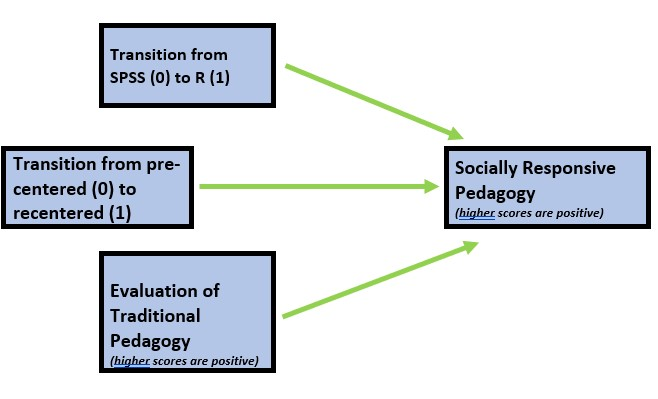
\includegraphics{Worked_Examples/images/homeworked_model.jpg}
\caption{An image of our the prediction model for the homeworked example.}
\end{figure}

\hypertarget{import-data-1}{%
\subsubsection*{Import data}\label{import-data-1}}


\begin{Shaded}
\begin{Highlighting}[]
\NormalTok{raw }\OtherTok{\textless{}{-}} \FunctionTok{readRDS}\NormalTok{(}\StringTok{"ReC.rds"}\NormalTok{)}
\FunctionTok{nrow}\NormalTok{(raw)}
\end{Highlighting}
\end{Shaded}

\begin{verbatim}
[1] 310
\end{verbatim}

\hypertarget{apply-inclusionaryexclusionary-criteria}{%
\subsubsection*{Apply inclusionary/exclusionary criteria}\label{apply-inclusionaryexclusionary-criteria}}


Because this data is publicly posted on the Open Science Framework, it was necessary for me to already exclude those individuals. This data was unique in that students could freely write some version of ``Opt out.'' My original code included a handful of versions, but here was the basic form:

\begin{Shaded}
\begin{Highlighting}[]
\CommentTok{\# testing to see if my code worked raw \textless{}{-} dplyr::filter (raw,}
\CommentTok{\# SPFC.Decolonize.Opt.Out != \textquotesingle{}Okay\textquotesingle{})}
\NormalTok{raw }\OtherTok{\textless{}{-}}\NormalTok{ dplyr}\SpecialCharTok{::}\FunctionTok{filter}\NormalTok{(raw, SPFC.Decolonize.Opt.Out }\SpecialCharTok{!=} \StringTok{"Opt Out"}\NormalTok{)}
\end{Highlighting}
\end{Shaded}

I want to exclude students' responses for the ANOVA and psychometrics courses.

\begin{Shaded}
\begin{Highlighting}[]
\NormalTok{raw }\OtherTok{\textless{}{-}}\NormalTok{ dplyr}\SpecialCharTok{::}\FunctionTok{filter}\NormalTok{(raw, Course }\SpecialCharTok{==} \StringTok{"Multivariate"}\NormalTok{)}
\end{Highlighting}
\end{Shaded}

At this point, these my only inclusion/exclusion criteria. I can determine how many students (who consented) completed any portion of the survey.

\begin{Shaded}
\begin{Highlighting}[]
\FunctionTok{nrow}\NormalTok{(raw)}
\end{Highlighting}
\end{Shaded}

\begin{verbatim}
[1] 84
\end{verbatim}

\hypertarget{format-any-variables-that-shouldnt-be-imputed-in-their-raw-form}{%
\subsubsection{Format any variables that shouldn't be imputed in their raw form}\label{format-any-variables-that-shouldnt-be-imputed-in-their-raw-form}}

Let's first create a df with the item-level variables that will fuel our model.

In addition to the variables in our model, we will include four auxiliary variables. These include Dept (Department: Clinical or Industrial-Organizational) and four additional course evaluation items: OvInstructor, MyContribution, IncrInterest, IncrUnderstanding.

Let's check the structure to be certain that \emph{StatsPkg} (SPSS, R) and \emph{Centered} (Pre, Re) are ordered factors. We also want the course evaluation items to be integer (or numerical).

\begin{Shaded}
\begin{Highlighting}[]
\NormalTok{mimp\_df }\OtherTok{\textless{}{-}}\NormalTok{ dplyr}\SpecialCharTok{::}\FunctionTok{select}\NormalTok{(raw, deID, StatsPkg, Centering, ClearResponsibilities,}
\NormalTok{    EffectiveAnswers, Feedback, ClearOrganization, ClearPresentation, InclusvClassrm,}
\NormalTok{    EquitableEval, MultPerspectives, DEIintegration, Dept, OvInstructor,}
\NormalTok{    MyContribution, IncrInterest, IncrUnderstanding)}
\FunctionTok{str}\NormalTok{(mimp\_df)}
\end{Highlighting}
\end{Shaded}

\begin{verbatim}
Classes 'data.table' and 'data.frame':  84 obs. of  17 variables:
 $ deID                 : int  11 12 13 14 15 16 17 18 35 19 ...
 $ StatsPkg             : Factor w/ 2 levels "SPSS","R": 2 2 2 2 2 2 2 2 2 2 ...
 $ Centering            : Factor w/ 2 levels "Pre","Re": 2 2 2 2 2 2 2 2 2 2 ...
 $ ClearResponsibilities: int  4 5 5 5 4 3 5 5 3 5 ...
 $ EffectiveAnswers     : int  4 5 5 4 4 3 5 5 4 4 ...
 $ Feedback             : int  4 5 4 4 5 4 5 4 4 5 ...
 $ ClearOrganization    : int  3 5 5 4 4 3 5 5 4 5 ...
 $ ClearPresentation    : int  4 5 5 3 4 2 5 4 5 5 ...
 $ InclusvClassrm       : int  5 5 5 5 5 4 5 5 5 5 ...
 $ EquitableEval        : int  4 5 5 5 4 4 5 4 5 5 ...
 $ MultPerspectives     : int  4 5 5 5 5 5 5 4 5 5 ...
 $ DEIintegration       : int  5 5 5 5 5 5 5 5 5 5 ...
 $ Dept                 : chr  "CPY" "CPY" "CPY" "CPY" ...
 $ OvInstructor         : int  3 5 5 3 5 2 5 4 5 5 ...
 $ MyContribution       : int  4 5 4 3 4 3 5 4 4 5 ...
 $ IncrInterest         : int  4 5 4 3 4 3 5 4 5 4 ...
 $ IncrUnderstanding    : int  4 5 5 3 4 3 5 4 5 5 ...
 - attr(*, ".internal.selfref")=<externalptr> 
\end{verbatim}

\begin{Shaded}
\begin{Highlighting}[]
\NormalTok{mimp\_df}\SpecialCharTok{$}\NormalTok{Dept }\OtherTok{\textless{}{-}} \FunctionTok{factor}\NormalTok{(mimp\_df}\SpecialCharTok{$}\NormalTok{Dept, }\AttributeTok{levels =} \FunctionTok{c}\NormalTok{(}\StringTok{"CPY"}\NormalTok{, }\StringTok{"ORG"}\NormalTok{))}
\FunctionTok{str}\NormalTok{(mimp\_df}\SpecialCharTok{$}\NormalTok{Dept)}
\end{Highlighting}
\end{Shaded}

\begin{verbatim}
 Factor w/ 2 levels "CPY","ORG": 1 1 1 1 1 1 1 1 1 1 ...
\end{verbatim}

We should eliminate case with greater than 50\% missingness.

\begin{Shaded}
\begin{Highlighting}[]
\FunctionTok{library}\NormalTok{(tidyverse)}
\CommentTok{\#Calculating number and proportion of item{-}level missingness}
\NormalTok{mimp\_df}\SpecialCharTok{$}\NormalTok{nmiss }\OtherTok{\textless{}{-}}\NormalTok{ mimp\_df}\SpecialCharTok{\%\textgreater{}\%}
\NormalTok{    dplyr}\SpecialCharTok{::}\FunctionTok{select}\NormalTok{(StatsPkg}\SpecialCharTok{:}\NormalTok{IncrUnderstanding) }\SpecialCharTok{\%\textgreater{}\%} \CommentTok{\#the colon allows us to include all variables between the two listed (the variables need to be in order)}
\NormalTok{    is.na }\SpecialCharTok{\%\textgreater{}\%} 
\NormalTok{    rowSums}

\NormalTok{mimp\_df}\OtherTok{\textless{}{-}}\NormalTok{ mimp\_df}\SpecialCharTok{\%\textgreater{}\%}
\NormalTok{  dplyr}\SpecialCharTok{::}\FunctionTok{mutate}\NormalTok{(}\AttributeTok{prop\_miss =}\NormalTok{ (nmiss}\SpecialCharTok{/}\DecValTok{13}\NormalTok{)}\SpecialCharTok{*}\DecValTok{100}\NormalTok{) }\CommentTok{\#11 is the number of variables included in calculating the proportion}

\NormalTok{mimp\_df }\OtherTok{\textless{}{-}} \FunctionTok{filter}\NormalTok{(mimp\_df, prop\_miss }\SpecialCharTok{\textless{}=} \DecValTok{50}\NormalTok{)  }\CommentTok{\#update df to have only those with at least 50\% of complete data}
\end{Highlighting}
\end{Shaded}

Once again, trim the df to include only the data to be included in the imputation

\begin{Shaded}
\begin{Highlighting}[]
\NormalTok{mimp\_df }\OtherTok{\textless{}{-}}\NormalTok{  dplyr}\SpecialCharTok{::}\FunctionTok{select}\NormalTok{(mimp\_df, deID, StatsPkg, Centering,ClearResponsibilities, EffectiveAnswers, Feedback, ClearOrganization, ClearPresentation, InclusvClassrm, EquitableEval, MultPerspectives, DEIintegration, Dept, OvInstructor, MyContribution, IncrInterest, IncrUnderstanding)}
\end{Highlighting}
\end{Shaded}

\hypertarget{multiply-impute-a-minimum-of-5-sets-of-data}{%
\subsubsection{Multiply impute a minimum of 5 sets of data}\label{multiply-impute-a-minimum-of-5-sets-of-data}}

Because multiple imputation is a \emph{random} process, if we all want the same answers we need to set a \emph{random seed.}

\begin{Shaded}
\begin{Highlighting}[]
\FunctionTok{set.seed}\NormalTok{(}\DecValTok{2309034}\NormalTok{)  }\CommentTok{\#you can pick any number you want, today I\textquotesingle{}m using today\textquotesingle{}s datestamp}
\end{Highlighting}
\end{Shaded}

The program we will use is \emph{mice}. \emph{mice} assumes that each variable has a distribution and it imputes missing variables according to that distribution.

This means we need to correctly specify each variable's format/role. \emph{mice} will automatically choose a distribution (think ``format'') for each variable; we can override this by changing the methods' characteristics.

The following code sets up the structure for the imputation. This follows the Katitas example.

\begin{Shaded}
\begin{Highlighting}[]
\FunctionTok{library}\NormalTok{(mice)}
\CommentTok{\# runs the mice code with 0 iterations}
\NormalTok{imp }\OtherTok{\textless{}{-}} \FunctionTok{mice}\NormalTok{(mimp\_df, }\AttributeTok{maxit =} \DecValTok{0}\NormalTok{)}
\CommentTok{\# Extract predictor Matrix and methods of imputation}
\NormalTok{predM }\OtherTok{=}\NormalTok{ imp}\SpecialCharTok{$}\NormalTok{predictorMatrix}
\NormalTok{meth }\OtherTok{=}\NormalTok{ imp}\SpecialCharTok{$}\NormalTok{method}
\NormalTok{log }\OtherTok{=}\NormalTok{ imp}\SpecialCharTok{$}\NormalTok{log}
\end{Highlighting}
\end{Shaded}

Here we code what format/role each variable should be.

\begin{Shaded}
\begin{Highlighting}[]
\CommentTok{\# These variables are left in the dataset, but setting them = 0 means}
\CommentTok{\# they are not used as predictors.  We want our ID to be retained in}
\CommentTok{\# the df.  There\textquotesingle{}s nothing missing from it, and we don\textquotesingle{}t want it used}
\CommentTok{\# as a predictor, so it will just hang out.}
\NormalTok{predM[, }\FunctionTok{c}\NormalTok{(}\StringTok{"deID"}\NormalTok{)] }\OtherTok{=} \DecValTok{0}

\CommentTok{\# If you like, view the first few rows of the predictor matrix}
\CommentTok{\# head(predM)}

\CommentTok{\# We don\textquotesingle{}t have any ordered categorical variables, but if we did we}
\CommentTok{\# would follow this format poly \textless{}{-} c(\textquotesingle{}Var1\textquotesingle{}, \textquotesingle{}Var2\textquotesingle{})}

\CommentTok{\# We have three dichotomous variables}
\NormalTok{log }\OtherTok{\textless{}{-}} \FunctionTok{c}\NormalTok{(}\StringTok{"StatsPkg"}\NormalTok{, }\StringTok{"Centering"}\NormalTok{, }\StringTok{"Dept"}\NormalTok{)}

\CommentTok{\# Unordered categorical variables (nominal variables), but if we did}
\CommentTok{\# we would follow this format poly2 \textless{}{-} c(\textquotesingle{}format\textquotesingle{})}

\CommentTok{\# Turn their methods matrix into the specified imputation models}
\CommentTok{\# Remove the hashtag if you have any of these variables meth[poly] =}
\CommentTok{\# \textquotesingle{}polr\textquotesingle{}}
\NormalTok{meth[log] }\OtherTok{=} \StringTok{"logreg"}
\CommentTok{\# meth[poly2] = \textquotesingle{}polyreg\textquotesingle{}}

\NormalTok{meth}
\end{Highlighting}
\end{Shaded}

\begin{verbatim}
                 deID              StatsPkg             Centering 
                   ""              "logreg"              "logreg" 
ClearResponsibilities      EffectiveAnswers              Feedback 
                "pmm"                    ""                 "pmm" 
    ClearOrganization     ClearPresentation        InclusvClassrm 
                   ""                    ""                 "pmm" 
        EquitableEval      MultPerspectives        DEIintegration 
                   ""                 "pmm"                 "pmm" 
                 Dept          OvInstructor        MyContribution 
             "logreg"                    ""                    "" 
         IncrInterest     IncrUnderstanding 
                "pmm"                    "" 
\end{verbatim}

This list (meth) contains all our variables; ``pmm'' is the default and is the ``predictive mean matching'' process used. We see that \emph{StatsPkg} and \emph{Centering} are noted as ``logreg.'' This is because they are dichotomous variables. If there is \emph{``\,``} underneath it means the data is complete. The data will be used in imputing other data, but none of that data will be imputed.

Our variables of interest are now configured to be imputed with the imputation method we specified. Empty cells in the method matrix mean that those variables aren't going to be imputed.

If a variable has no missing values, it is automatically set to be empty. We can also manually set variables to not be imputed with the \emph{meth{[}variable{]}=``\,``} command.

The code below begins the imputation process. We are asking for 5 datasets. If you have many cases and many variables, this can take awhile. How many imputations? Recommendations have ranged as low as five to several hundred.

\begin{Shaded}
\begin{Highlighting}[]
\CommentTok{\# With this command, we tell mice to impute the anesimpor2 data,}
\CommentTok{\# create 5vvdatasets, use predM as the predictor matrix and don\textquotesingle{}t}
\CommentTok{\# print the imputation process.  If you would like to see the process}
\CommentTok{\# (or if the process is failing to execute) set print as TRUE; seeing}
\CommentTok{\# where the execution halts can point to problematic variables (more}
\CommentTok{\# notes at end of lecture)}

\NormalTok{imp2 }\OtherTok{\textless{}{-}} \FunctionTok{mice}\NormalTok{(mimp\_df, }\AttributeTok{maxit =} \DecValTok{5}\NormalTok{, }\AttributeTok{predictorMatrix =}\NormalTok{ predM, }\AttributeTok{method =}\NormalTok{ meth,}
    \AttributeTok{log =}\NormalTok{ log, }\AttributeTok{print =} \ConstantTok{FALSE}\NormalTok{)}
\end{Highlighting}
\end{Shaded}

We need to create a ``long file'' that stacks all the imputed data. Looking at the df in R Studio shows us that when imp = 0 (the pe-imputed data), there is still missingness. As we scroll through the remaining imputations, there are no NA cells.

\begin{Shaded}
\begin{Highlighting}[]
\CommentTok{\# First, turn the datasets into long format This procedure is, best I}
\CommentTok{\# can tell, unique to mice and wouldn\textquotesingle{}t work for repeated measures}
\CommentTok{\# designs}
\NormalTok{mimp\_long }\OtherTok{\textless{}{-}}\NormalTok{ mice}\SpecialCharTok{::}\FunctionTok{complete}\NormalTok{(imp2, }\AttributeTok{action =} \StringTok{"long"}\NormalTok{, }\AttributeTok{include =} \ConstantTok{TRUE}\NormalTok{)}
\end{Highlighting}
\end{Shaded}

If we look at it, we can see 6 sets of data. If the \emph{deID} variable is sorted we see that:

\begin{itemize}
\tightlist
\item
  .imp = 0 is the unimputed set; there are still missing values
\item
  .imp = 1, 2, 3, or 5 has no missing values for the variables we included in the imputation
\end{itemize}

With the code below we can see the proportion of missingness for each variable (that has missing data), sorted from highest to lowest.

\begin{Shaded}
\begin{Highlighting}[]
\NormalTok{p\_missing\_mimp\_long }\OtherTok{\textless{}{-}} \FunctionTok{unlist}\NormalTok{(}\FunctionTok{lapply}\NormalTok{(mimp\_long, }\ControlFlowTok{function}\NormalTok{(x) }\FunctionTok{sum}\NormalTok{(}\FunctionTok{is.na}\NormalTok{(x))))}\SpecialCharTok{/}\FunctionTok{nrow}\NormalTok{(mimp\_long)}
\FunctionTok{sort}\NormalTok{(p\_missing\_mimp\_long[p\_missing\_mimp\_long }\SpecialCharTok{\textgreater{}} \DecValTok{0}\NormalTok{], }\AttributeTok{decreasing =} \ConstantTok{TRUE}\NormalTok{)  }\CommentTok{\#check to see if this works}
\end{Highlighting}
\end{Shaded}

\begin{verbatim}
       DEIintegration        InclusvClassrm              Feedback 
          0.027777778           0.007936508           0.003968254 
ClearResponsibilities      MultPerspectives          IncrInterest 
          0.001984127           0.001984127           0.001984127 
\end{verbatim}

Because our imputation was item-level, we need to score the variables with scales/subscales.

Traditional pedagogy is a predictor variable that needs to be created by calculating the mean if at least 75\% of the items are non-missing. None of the items need to be reverse-scored. I will return to working with the \emph{scrub\_df} data.

\begin{Shaded}
\begin{Highlighting}[]
\CommentTok{\# this seems to work when I build the book, but not in \textquotesingle{}working the}
\CommentTok{\# problem\textquotesingle{}}
\NormalTok{TradPed\_vars }\OtherTok{\textless{}{-}} \FunctionTok{c}\NormalTok{(}\StringTok{"ClearResponsibilities"}\NormalTok{, }\StringTok{"EffectiveAnswers"}\NormalTok{, }\StringTok{"Feedback"}\NormalTok{,}
    \StringTok{"ClearOrganization"}\NormalTok{, }\StringTok{"ClearPresentation"}\NormalTok{)}
\CommentTok{\# mimp\_long$TradPed \textless{}{-} sjstats::mean\_n(mimp\_long[, TradPed\_vars],}
\CommentTok{\# .75)}

\CommentTok{\# this seems to work when I \textquotesingle{}work the problem\textquotesingle{} (but not when I build}
\CommentTok{\# the book) the difference is the two dots before the last SRPed\_vars}
\NormalTok{mimp\_long}\SpecialCharTok{$}\NormalTok{TradPed }\OtherTok{\textless{}{-}}\NormalTok{ sjstats}\SpecialCharTok{::}\FunctionTok{mean\_n}\NormalTok{(mimp\_long[, TradPed\_vars], }\FloatTok{0.75}\NormalTok{)}
\end{Highlighting}
\end{Shaded}

The dependent variable is socially responsive pedagogy. It needs to be created by calculating the mean if at least 75\% of the items are non-missing. None of the items need to be reverse-scored.

\begin{Shaded}
\begin{Highlighting}[]
\CommentTok{\# this seems to work when I build the book, but not in \textquotesingle{}working the}
\CommentTok{\# problem\textquotesingle{} SRPed\_vars \textless{}{-} c(\textquotesingle{}InclusvClassrm\textquotesingle{},\textquotesingle{}EquitableEval\textquotesingle{},}
\CommentTok{\# \textquotesingle{}MultPerspectives\textquotesingle{}, \textquotesingle{}DEIintegration\textquotesingle{}) mimp\_long$SRPed \textless{}{-}}
\CommentTok{\# sjstats::mean\_n(mimp\_long[, SRPed\_vars], .75)}

\CommentTok{\# this seems to work when I \textquotesingle{}work the problem\textquotesingle{} (but not when I build}
\CommentTok{\# the book) the difference is the two dots before the last SRPed\_vars}
\NormalTok{SRPed\_vars }\OtherTok{\textless{}{-}} \FunctionTok{c}\NormalTok{(}\StringTok{"InclusvClassrm"}\NormalTok{, }\StringTok{"EquitableEval"}\NormalTok{, }\StringTok{"MultPerspectives"}\NormalTok{,}
    \StringTok{"DEIintegration"}\NormalTok{)}
\NormalTok{mimp\_long}\SpecialCharTok{$}\NormalTok{SRPed }\OtherTok{\textless{}{-}}\NormalTok{ sjstats}\SpecialCharTok{::}\FunctionTok{mean\_n}\NormalTok{(mimp\_long[, SRPed\_vars], }\FloatTok{0.75}\NormalTok{)}
\end{Highlighting}
\end{Shaded}

\hypertarget{run-a-regression-for-multiply-imputed-data-with-at-least-three-variables}{%
\subsubsection{Run a regression (for multiply imputed data) with at least three variables}\label{run-a-regression-for-multiply-imputed-data-with-at-least-three-variables}}

For comparison, here was the script when we used the AIA approach for managing missingness:

\begin{quote}
\begin{quote}
SRPed\_fit \textless- lm(SRPed \textasciitilde{} StatsPkg + Centering + TradPed, data = scored)
\end{quote}
\end{quote}

In order for the regression to use multiply imputed data, it must be a ``mids'' (multiply imputed data sets) type

\begin{Shaded}
\begin{Highlighting}[]
\CommentTok{\# Convert to mids type {-} mice can work with this type}
\NormalTok{mimp\_mids }\OtherTok{\textless{}{-}} \FunctionTok{as.mids}\NormalTok{(mimp\_long)}
\end{Highlighting}
\end{Shaded}

Here's what we do with imputed data:

\begin{Shaded}
\begin{Highlighting}[]
\NormalTok{fitimp }\OtherTok{\textless{}{-}} \FunctionTok{with}\NormalTok{(mimp\_mids, }\FunctionTok{lm}\NormalTok{(SRPed }\SpecialCharTok{\textasciitilde{}}\NormalTok{ StatsPkg }\SpecialCharTok{+}\NormalTok{ Centering }\SpecialCharTok{+}\NormalTok{ TradPed))}
\end{Highlighting}
\end{Shaded}

In this process, 5 individual, OLS, regressions are being conducted and the results being pooled into this single set.

\begin{Shaded}
\begin{Highlighting}[]
\CommentTok{\# to get the 5, individual imputations}
\FunctionTok{summary}\NormalTok{(fitimp)}
\end{Highlighting}
\end{Shaded}

\begin{verbatim}
# A tibble: 20 x 6
   term        estimate std.error statistic  p.value  nobs
   <chr>          <dbl>     <dbl>     <dbl>    <dbl> <int>
 1 (Intercept)    1.90     0.310      6.13  3.13e- 8    84
 2 StatsPkgR      0.187    0.118      1.59  1.16e- 1    84
 3 CenteringRe    0.117    0.108      1.09  2.79e- 1    84
 4 TradPed        0.565    0.0659     8.56  6.30e-13    84
 5 (Intercept)    1.94     0.314      6.17  2.62e- 8    84
 6 StatsPkgR      0.191    0.119      1.60  1.13e- 1    84
 7 CenteringRe    0.110    0.109      1.01  3.17e- 1    84
 8 TradPed        0.557    0.0667     8.36  1.63e-12    84
 9 (Intercept)    1.96     0.313      6.26  1.80e- 8    84
10 StatsPkgR      0.178    0.119      1.50  1.38e- 1    84
11 CenteringRe    0.111    0.109      1.02  3.10e- 1    84
12 TradPed        0.555    0.0665     8.35  1.69e-12    84
13 (Intercept)    2.03     0.325      6.24  1.98e- 8    84
14 StatsPkgR      0.185    0.123      1.50  1.38e- 1    84
15 CenteringRe    0.104    0.113      0.918 3.62e- 1    84
16 TradPed        0.539    0.0691     7.80  1.95e-11    84
17 (Intercept)    1.91     0.306      6.26  1.77e- 8    84
18 StatsPkgR      0.158    0.116      1.36  1.78e- 1    84
19 CenteringRe    0.117    0.107      1.10  2.76e- 1    84
20 TradPed        0.567    0.0649     8.73  2.93e-13    84
\end{verbatim}

\begin{Shaded}
\begin{Highlighting}[]
\FunctionTok{summary}\NormalTok{(}\FunctionTok{pool}\NormalTok{(fitimp))}
\end{Highlighting}
\end{Shaded}

\begin{verbatim}
         term  estimate  std.error statistic       df              p.value
1 (Intercept) 1.9480744 0.31833535  6.119567 74.55114 0.000000040039269753
2   StatsPkgR 0.1798400 0.11996611  1.499090 76.64577 0.137957984459613908
3 CenteringRe 0.1117906 0.10918108  1.023901 77.81162 0.309054914517060075
4     TradPed 0.5564494 0.06768356  8.221338 74.26455 0.000000000004825124
\end{verbatim}

\begin{quote}
\begin{quote}
Results of a multiple regression predicting the socially responsive course evaluation ratings indicated that neither the transition from SPSS to R (\(B = 0.178, p = 0.135\)) nor the transition to an explicitly recentered curriculum (\(B = 0.116, p = 0.285) led to statistically significant diferences. In contrast, traditional pedagogy had a strong, positive effect on evaluations of socially responsive pedagogy (\)B = 0.571, p \textless{} 0.001). Results of the regression model are presented in Table 2.
\end{quote}
\end{quote}

\hypertarget{apa-style-write-up-of-the-multiple-imputation-section-of-data-diagnostics}{%
\subsubsection{APA style write-up of the multiple imputation section of data diagnostics}\label{apa-style-write-up-of-the-multiple-imputation-section-of-data-diagnostics}}

My write-up draws from some of the results we obtained in the homeworked example at the end of the \protect\hyperlink{DataDx}{Data Dx} chapter.

\begin{quote}
\begin{quote}
This is a secondary analysis of data involved in a more comprehensive dataset that included students taking multiple statistics courses (\emph{N} = 310). Having retrieved this data from a repository in the Open Science Framework, only those who consented to participation in the study were included. Data used in these analyses were 84 students who completed the multivariate clas.
\end{quote}
\end{quote}

\begin{quote}
\begin{quote}
Across cases that were deemed eligible on the basis of the inclusion/exclusion criteria, missingness ranged from 0 to 100\%. Across the dataset, 3.86\% of cells had missing data and 87.88\% of cases had nonmissing data. At this stage in the analysis, missingness for all cases did not exceed 50\% \citep{katitas_getting_2019} and they were all included in the multiple imputation .
\end{quote}
\end{quote}

\begin{quote}
\begin{quote}
Regarding the distributional characteristics of the data, skew and kurtosis values of the variables fell below the values of 3 (skew) and 10 (kurtosis) that Kline suggests are concerning \citeyearpar{kline_principles_2016}. Results of the Shapiro-Wilk test of normality indicate that our variables assessing the traditional pedagogy (\(W = 0.830, p < 0.001\)) and socially responsive pedagogy (0.818, p \textless{} 0.001) are statistically significantly different than a normal distribution. Inspection of distributions of the variables indicated that both course evaluation variables were negatively skewed, with a large proportion of high scores.
\end{quote}
\end{quote}

\begin{quote}
\begin{quote}
We evaluated multivariate normality with the Mahalanobis distance test. Specifically, we used the \emph{psych::outlier()} function and included both continuous variables in the calculation. Our visual inspection of the Q-Q plot suggested that the plotted line strayed from the straight line as the quantiles increased. Additionally, we appended the Mahalanobis distance scores as a variable to the data. Analyzing this variable, we found that 2 cases exceed three standard deviations beyond the median.
\end{quote}
\end{quote}

\begin{quote}
\begin{quote}
We managed missing data with multiple imputation \citep{enders_multiple_2017, katitas_getting_2019}. We imputed five sets of data with the R package, \emph{mice} (v. 3.13) -- a program that utilizes conditional multiple imputation. The imputation included the 9 item-level variables that comprised our scales and the dichotomous variable representing traditional pedagogy and socially responsive pedagogy. We also included five auxiliary variables (four variables from the course evaluation and the whether the student was from the Clinical or Industrial-Organizational Psychology program).
\end{quote}
\end{quote}

\hypertarget{apa-style-write-up-regression-results}{%
\subsubsection{APA style write-up regression results}\label{apa-style-write-up-regression-results}}

\begin{quote}
\begin{quote}
Results of a multiple regression predicting the socially responsive course evaluation ratings indicated that neither the transition from SPSS to R (\(B = 0.178, p = 0.135\)) nor the transition to an explicitly recentered curriculum (\(B = 0.116, p = 0.285) led to statistically significant diferences. In contrast, traditional pedagogy had a strong, positive effect on evaluations of socially responsive pedagogy (\)B = 0.571, p \textless{} 0.001). Results of the regression model are presented in Table 2.
\end{quote}
\end{quote}

\emph{As in the lesson itself, I used the data diagnostics that we did in the AIA method. It feels to me like these should be calculated with the multiply imputed data (i.e., 5 sets, with pooled estimates and standard errors), but I do not see that modeled -- anywhere in tutorials I consulted.}

\hypertarget{MED}{%
\chapter*{MEDIATION}\label{MED}}


\hypertarget{SimpleMed}{%
\chapter{Simple Mediation}\label{SimpleMed}}

\href{https://spu.hosted.panopto.com/Panopto/Pages/Viewer.aspx?pid=7ffb03e6-b34b-4e0b-8f10-ad080180b069}{Screencasted Lecture Link}

The focus of this lecture is to estimate indirect effects (aka ``mediation''). We examine the logic/design required to support the argument that \emph{mediation} is the \emph{mechanism} that explains the X --\textgreater{} Y relationship. We also work three examples (one with covariates).

At the outset, please note that although I rely heavily on Hayes \citeyearpar{hayes_introduction_2018} text and materials, I am using the R package \emph{lavaan} in these chapters. Very recently, Hayes has introduced a \href{https://www.processmacro.org/index.html}{PROCESS macro for R}. Because I am not yet up-to-speed on using this macro (it is not a typical R package) and because we will use \emph{lavaan} for confirmatory factor analysis and structural equation modeling, I have chosen to utilize the \emph{lavaan} package. A substantial difference is that the PROCESS macros use ordinary least squares and \emph{lavaan} uses maximum likelihood estimators.

\hypertarget{navigating-this-lesson-4}{%
\section{Navigating this Lesson}\label{navigating-this-lesson-4}}

There is about 1 hour and 10 minutes of lecture. If you work through the materials with me it would be plan for an additional 1.5 hours.

While the majority of R objects and data you will need are created within the R script that sources the chapter, ocasionally there are some that cannot be created from within the R framework. Additionally, sometimes links fail. All original materials are provided at the \href{https://github.com/lhbikos/ReC_MultivModel}{Github site} that hosts the book. More detailed guidelines for ways to access all these materials are provided in the OER's \protect\hyperlink{ReCintro}{introduction}

\hypertarget{learning-objectives-4}{%
\subsection{Learning Objectives}\label{learning-objectives-4}}

Learning objectives from this lecture include the following:

\begin{itemize}
\tightlist
\item
  Define mediation and indirect effect.
\item
  Distinguish the role of a mediating variable from independent variables, covariates, and moderators.
\item
  Identify the conditions upon which there can be justification to support the presence of a mediated effect.
\item
  Articulate the arguments for and against using the term, ``mediation.''
\item
  Using the R package \emph{lavaan},

  \begin{itemize}
  \tightlist
  \item
    specify a model with indirect effects,
  \item
    identify and interpret B weights, \emph{p} values, and \emph{CIs} for total, direct, and indirect effects,
  \item
    calculate the total effects of X and M on Y,
  \item
    identify the proportion of variance accounted for in predicting M and Y.
  \end{itemize}
\item
  Hand calculate the values of an indirect, direct, and total effects from statistical output or a figure (just the \(B\) or \(\beta\), not the significance level)
\end{itemize}

\hypertarget{planning-for-practice-4}{%
\subsection{Planning for Practice}\label{planning-for-practice-4}}

The following suggestions for practice will involve specifying, testing, and interpreting a model with a single indirect effect (mediator).

\begin{itemize}
\tightlist
\item
  Rework the problem in the chapter by changing the random seed in the code that simulates the data. This should provide minor changes to the data, but the results will likely be very similar.
\item
  There are a number of variables in the dataset and there were a handful of simple mediations conducted in the journal article that sources the research vignette. Swap out one or more variables in the model of simple mediation and compare your solution to the one in the chapter and/or the research article.
\item
  Conduct a simple mediation with data to which you have access. This could include data you simulate on your own or from a published article.
\end{itemize}

\hypertarget{readings-resources-4}{%
\subsection{Readings \& Resources}\label{readings-resources-4}}

In preparing this chapter, I drew heavily from the following resource(s). Other resources are cited (when possible, linked) in the text with complete citations in the reference list.

\begin{itemize}
\tightlist
\item
  Hayes, A. F. (2018). \emph{Introduction to mediation, moderation, and conditional process anlaysis: A regression-based approach}. New York, NY: Guilford Press. Available as an ebook from the SPU library: \url{https://ebookcentral-proquest-com.ezproxy.spu.edu/lib/spu/detail.action?docID=5109647}

  \begin{itemize}
  \tightlist
  \item
    \textbf{Chapter 3, Simple mediation}: Hayes' text is another great example of a teaching tool that is accessible at both procedural and conceptual levels. I especially appreciate his attention to the controversies (even those directed toward his work). We deviate from his text in that we are not using the PROCESS macro\ldots and I'll address those concerns in the lecture.
  \item
    \textbf{Chapter 4, Causality and confounds}: A great chapter that addresses ``What happened to Baron \& Kenny''; partial v complete mediation; and conditions required for claims of causality. Procedurally, our focus in this chapter is on the role of covariates.
  \item
    \textbf{Appendix A: Using Process}: An essential tool for PROCESS users because, even when we are in the R environment, this is the ``idea book.'' That is, the place where all the path models are presented in figures.
  \end{itemize}
\item
  Kim, P. Y., Kendall, D. L., \& Cheon, H.-S. (2017). Racial microaggressions, cultural mistrust, and mental health outcomes among Asian American college students. \emph{American Journal of Orthopsychiatry, 87}(6), 663--670. \url{https://doi-org.ezproxy.spu.edu/10.1037/ort0000203}
\end{itemize}

\hypertarget{packages-4}{%
\subsection{Packages}\label{packages-4}}

The script below will (a) check to see if the following packages are installed on your computer and, if not (b) install them.

\begin{Shaded}
\begin{Highlighting}[]
\CommentTok{\#will install the package if not already installed}
\ControlFlowTok{if}\NormalTok{(}\SpecialCharTok{!}\FunctionTok{require}\NormalTok{(lavaan))\{}\FunctionTok{install.packages}\NormalTok{(}\StringTok{"lavaan"}\NormalTok{)\}}
\ControlFlowTok{if}\NormalTok{(}\SpecialCharTok{!}\FunctionTok{require}\NormalTok{(semPlot))\{}\FunctionTok{install.packages}\NormalTok{(}\StringTok{"semPlot"}\NormalTok{)\}}
\ControlFlowTok{if}\NormalTok{(}\SpecialCharTok{!}\FunctionTok{require}\NormalTok{(tidyverse))\{}\FunctionTok{install.packages}\NormalTok{(}\StringTok{"tidyverse"}\NormalTok{)\}}
\ControlFlowTok{if}\NormalTok{(}\SpecialCharTok{!}\FunctionTok{require}\NormalTok{(psych))\{}\FunctionTok{install.packages}\NormalTok{(}\StringTok{"psych"}\NormalTok{)\}}
\ControlFlowTok{if}\NormalTok{(}\SpecialCharTok{!}\FunctionTok{require}\NormalTok{(formattable))\{}\FunctionTok{install.packages}\NormalTok{(}\StringTok{"formattable"}\NormalTok{)\}}
\ControlFlowTok{if}\NormalTok{(}\SpecialCharTok{!}\FunctionTok{require}\NormalTok{(semTable))\{}\FunctionTok{install.packages}\NormalTok{(}\StringTok{"semTable"}\NormalTok{)\}}
\end{Highlighting}
\end{Shaded}

\hypertarget{estimating-indirect-effects-the-analytic-approach-often-termed-mediation}{%
\section{\texorpdfstring{Estimating Indirect Effects (the analytic approach often termed \emph{mediation})}{Estimating Indirect Effects (the analytic approach often termed mediation)}}\label{estimating-indirect-effects-the-analytic-approach-often-termed-mediation}}

\hypertarget{the-definitional-and-conceptual}{%
\subsection{The definitional and conceptual}\label{the-definitional-and-conceptual}}

As in Hayes text \citeyearpar{hayes_introduction_2018}, we will differentiate between \emph{moderation} and \emph{mediation}. \emph{Conditional process analysis} involves both! With each of these, we are seeking to understand the \emph{mechanism} at work that leads to the relationship (be it correlational, predictive, or causal)

Even though this process has sometimes been termed \emph{causal modeling}, Hayes argues that his \emph{statistical approach} is not claiming to determine \emph{cause}; that is really left to the argument of the research design.

\textbf{Moderation} (a review):

\begin{itemize}
\tightlist
\item
  Answers questions of \emph{when} or \emph{for whom} and is often the source of the answer, \emph{it depends}.
\item
  Think of our \emph{interaction} effects in ANOVA and regression
\item
  The effect of X on some variable Y is moderated by W if its size, sign, or strength depends on, or can be predicted, by W. Then we can say, ``W is a \emph{moderator} of X's effect on Y'' or ``W and X \emph{interact} in their influence on Y.''
\item
  The image below illustrates moderation with \emph{conceptual} and \emph{statistical} diagrams. Note that three predictors (IV, DV, their interaction) point to the DV.
\end{itemize}

\begin{figure}
\centering
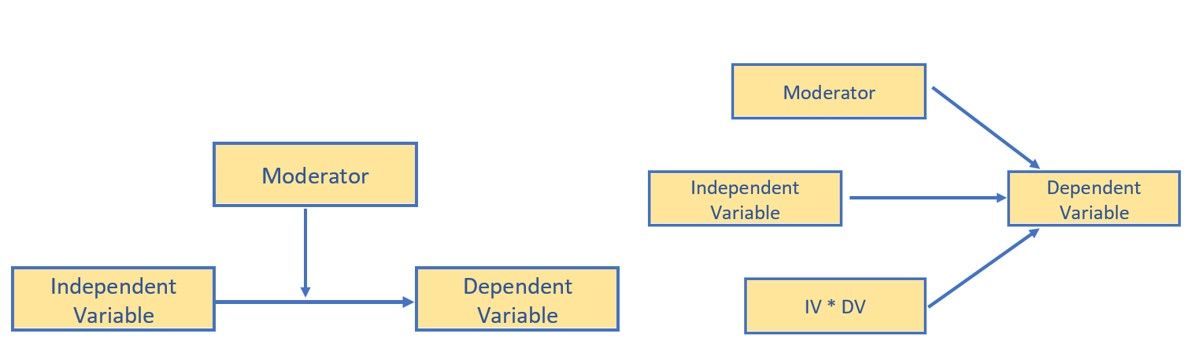
\includegraphics{images/SimpleMed/ModConcStat.jpg}
\caption{Image of Hayes'style conceptual and statistical diagrams of a simple moderation}
\end{figure}

The classic plot of moderation results is often the best way to detect that an interaction was included in the analysis and helps understand the \emph{conditional} (e.g., for whom, under what conditions) nature of the analysis.

\begin{figure}
\centering
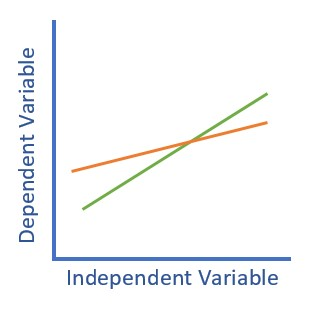
\includegraphics{images/SimpleMed/SimpleInteraction.jpg}
\caption{Image of classic interaction graph that illustrates a moderated effect. The IV is on the X axis, DV on the Y axis, and two intersecting lines represent the differential/moderated effect of the IV on the DV by the moderator}
\end{figure}

\textbf{Mediation}:

\begin{itemize}
\tightlist
\item
  Answers questions of \emph{how} (I also think \emph{through} and \emph{via} to describe the proposed mediating mechanism)
\item
  Paths in a mediation model are \emph{direct} (X does not pass through M on its way to Y) and \emph{indirect} (X passes through M on its way to Y). Once we get into the statistics, we will also be focused on \emph{total} effects.
\item
  Hayes thinks in terms of \emph{antecedent} and \emph{consequent} variables. In a 3-variable, simple mediation, X and M are the antecedent variables; X and M are the consequent variables.\\
\item
  There is substantial debate and controversy about whether we can say ``the effect of X on Y is \emph{mediated} through M'' or whether we should say, ``There is a statistically significant indirect effect of X on Y thru M.'' Hayes comes down on the ``use mediation language'' side of the debate.\\
\item
  In sum, a simple mediation model is any causal system in which at least one causal antecedent X variable is proposed as influencing an outcome Y through a single intervening variable, M. In such a model there are two pathways by which X can influence Y.
\item
  The figure below doubles as both the conceptual and statistical diagram of evaluating a simple mediation -- a simple indirect effect.
\end{itemize}

\begin{figure}
\centering
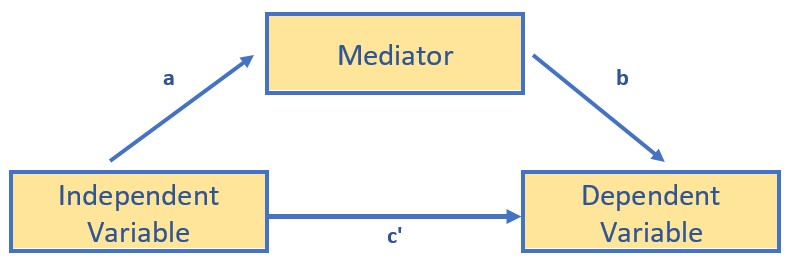
\includegraphics{images/SimpleMed/SimpleMed.jpg}
\caption{Image of Hayes'style conceptual diagram of a simple moderation}
\end{figure}

\textbf{Conditional process analysis}:

\begin{itemize}
\tightlist
\item
  Used when the research goal is to understand the boundary conditions of the mechanism(s) by which a variable transmits its effect on another.\\
\item
  Typically, simultaneously, assesses the influence of mediating (indirect effects) and moderating (interactional effects) in a model-building fashion.
\item
  In a conditional process model, the moderator(s) may be hypothesized to influence one or more of the paths.
\end{itemize}

We will work toward building a conditional process model, a moderated mediation, over the next several chapters.

\begin{figure}
\hypertarget{id}{%
\centering
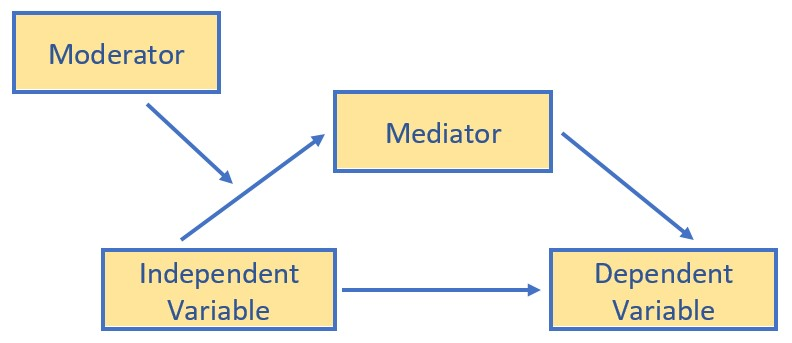
\includegraphics[width=2.60417in,height=1.875in]{images/SimpleMed/CPAmodel.jpg}
\caption{Image of conditional process analysis model where the moderator is hypothesized to change the a path; the path between the IV and mediator}\label{id}
}
\end{figure}

\hypertarget{workflow-for-simple-mediation}{%
\section{Workflow for Simple Mediation}\label{workflow-for-simple-mediation}}

The workflow for a simple mediation is straightforward, however the figure below (i.e., the very traditional figure used to represent mediation) is very helpful in understanding the logic beneath mediation as the explanatory mechanism.

\begin{figure}
\centering
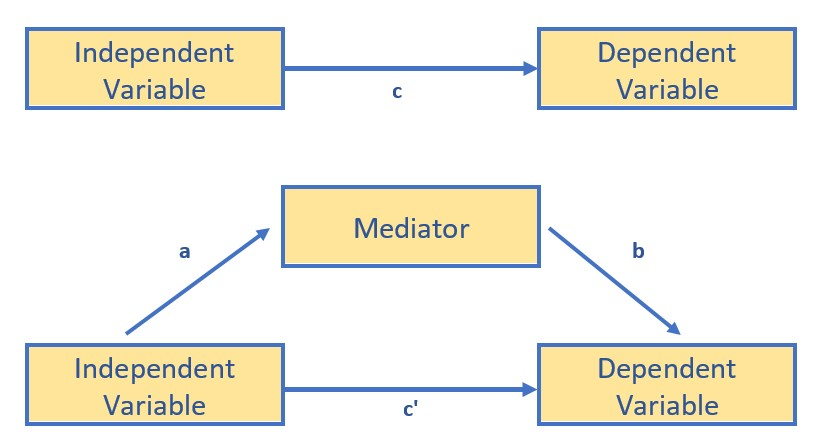
\includegraphics{images/SimpleMed/MedRationale.jpg}
\caption{Image of conditional process analysis model where the mediator is hypothesized to change the a path; the path between the IV and mediator}
\end{figure}

The top figure represents the bivariate relationship between the independent and dependent variable. The result of a simple linear regression (one predictor) represent the \emph{total} effect of the IV on the DV. We can calculate this by simply regressing the DV onto the IV. The resulting \(B\) weight is known as the \emph{c} path. A bivariate correlation coefficient results in the same value -- only it is standardized (so would be the same as the \(\beta\) weight).

The lower figure represents that the relationship between the IV and DV is \emph{mediated} by a third variable. We assign three labels to the paths: \emph{a}, between the IV and mediator; \emph{b}, between the mediator and DV; and \emph{c'} (c prime) between the IV and DV.

Statistically speaking, a mediated relationship is supported when the value of \emph{c'} is statistically significantly lower than \emph{c}. If this occurs, then we can say that the mediator is sharing some of the variance in the prediction of the DV.

You might already be imagining potential challenges to this model. For example, which variable should be the IV and which one should be the mediator? Can we switch them? You can -- and you will likely have very similar (if not identical) results. Good research design is what provides support for suggesting that mediation is the proper, casual, mechanism regarding the relationship between the IV and DV. An excellent review of the challenges of establishing a robust mediation model is provided by Kline \citeyearpar{kline_mediation_2015}, where he suggests the following as the minimally required elements of a mediation design:

\begin{itemize}
\tightlist
\item
  the IV is an experimental variable with random assignment to conditions;
\item
  the mediator is an individual difference variable that is not manipulated and is measured at a later time;and
\item
  the DV is measured at a third occasion
\end{itemize}

These criteria are in addition to the rather standard criteria for establishing causality \citep[see][ for a review]{stone-romero_research_2010}:

\begin{itemize}
\tightlist
\item
  temporal precedence,
\item
  statistical covariation, and
\item
  ruling out plausible rival hypotheses.
\end{itemize}

Some journals take this very seriously. In fact \href{https://www.journals.elsevier.com/journal-of-vocational-behavior/news/frequently-asked-questions-about-submitting-a-manuscript}{FAQs} in the Journal of Vocational Behavior make it clear that they will very rarely publish a ``mediation manuscript'' unless it has a minimum of three waves.

Working through a mediation will help operationalize these concepts.

\hypertarget{simple-mediation-in-lavaan-a-focus-on-the-mechanics}{%
\section{\texorpdfstring{Simple Mediation in \emph{lavaan}: A focus on the mechanics}{Simple Mediation in lavaan: A focus on the mechanics}}\label{simple-mediation-in-lavaan-a-focus-on-the-mechanics}}

The lavaan tutorial \citep{rosseel_lavaan_2020} provides a helpful model of how writing code to estimate an indirect effect. Using the lavaan tutorial as our guide, let's start with just a set of fake data with variable names that represent X (predictor, IV, antecedent), M (mediator, atencedent, consequent), and Y (outcome, DV, consequent).

\hypertarget{simulate-fake-data}{%
\subsection{Simulate Fake Data}\label{simulate-fake-data}}

The code below is asking to create a dataset with a sample size of 100. The dataset has 3 variables, conveniently named X (predictor, antecedent, IV), M (mediator), and Y (outome, consequent, DV). The R code asks for random selection of numbers with a normal distribution. You can see that the M variable will be related to the X variable by + .5; and the Y variable will be related to the M variable by + .7. This rather ensures a statistically significant indirect effect.

\begin{Shaded}
\begin{Highlighting}[]
\FunctionTok{set.seed}\NormalTok{(}\DecValTok{210410}\NormalTok{)}
\NormalTok{X }\OtherTok{\textless{}{-}} \FunctionTok{rnorm}\NormalTok{(}\DecValTok{100}\NormalTok{)}
\NormalTok{M }\OtherTok{\textless{}{-}} \FloatTok{0.5}\SpecialCharTok{*}\NormalTok{X }\SpecialCharTok{+} \FunctionTok{rnorm}\NormalTok{(}\DecValTok{100}\NormalTok{)}
\NormalTok{Y }\OtherTok{\textless{}{-}} \FloatTok{0.7}\SpecialCharTok{*}\NormalTok{M }\SpecialCharTok{+} \FunctionTok{rnorm}\NormalTok{(}\DecValTok{100}\NormalTok{)}
\NormalTok{Data }\OtherTok{\textless{}{-}} \FunctionTok{data.frame}\NormalTok{(}\AttributeTok{X =}\NormalTok{ X, }\AttributeTok{Y =}\NormalTok{ Y, }\AttributeTok{M =}\NormalTok{ M)}
\end{Highlighting}
\end{Shaded}

\hypertarget{specify-mediation-model}{%
\subsection{Specify Mediation Model}\label{specify-mediation-model}}

The package we are using is \emph{lavaan}. Hayes' model is \emph{path analysis}, which can be a form of structural equation modeling. As a quick reminder, in SPSS, PROCESS is limited to ordinary least squares regression. We will use maximum likliehood estimators for the Hayes/PROCESS examples, but \emph{lavaan} can take us further than PROCESS because

\begin{itemize}
\tightlist
\item
  We can (and, in later chapters, will) do latent variable modeling.
\item
  We can have more specificity and flexibility than the prescribed PROCESS models allow. I say this with all due respect to Hayes -- there is also a good deal of flexibility to be able to add multiple mediators and covariates within most of the Hayes' prescribed models.
\end{itemize}

Hayes text is still a great place to start because the conceptual and procedural information is clear and transferable to the R environment.

\begin{Shaded}
\begin{Highlighting}[]
\FunctionTok{library}\NormalTok{(lavaan)}
\end{Highlighting}
\end{Shaded}

\begin{verbatim}
## This is lavaan 0.6-16
## lavaan is FREE software! Please report any bugs.
\end{verbatim}

Our atheoretical dataset makes it easy to identify which variable belongs in each role (X,Y,M). When specifying the paths in lavaan, here's what to keep in mind:

\begin{itemize}
\tightlist
\item
  Name your model/object (below is X, ``\textless-'' means ``is defined by'')
\item
  The model exists between 2 single quotation marks (the odd looking ' and ' at the beginning and end).
\item
  The \# of regression equations you need depends on the \# of variables that have arrows pointing to them. In a simple mediation, there are 3 variables with 2 variables having arrows pointing to them -- need 2 regression equations:

  \begin{itemize}
  \tightlist
  \item
    one for the Mediator
  \item
    one for the DV (Y)
  \end{itemize}
\item
  Operator for a regression analysis is the (tilde, \textasciitilde)
\item
  DV goes on left

  \begin{itemize}
  \tightlist
  \item
    In first equation we regress both the X and M onto Y
  \item
    In second equation we regress M onto X
  \end{itemize}
\item
  The asterisk (*) is a handy tool to label variables (don't confuse it as defining an interaction); this labeling as a, b, and c\_p (in traditional mediation, the total effect is labeled with a and the direct effect is c'{[}c prime{]}, but the script won't allow and extra single quotation mark, hence c\_p) is super helpful in interpreting the ouput
\item
  The indirect effect is created by multiplying the a and b paths.\\
\item
  The ``:='' sign is used when creating a new variable that is a function of variables in the model, but not in the dataset (i.e., the a and b path).
\end{itemize}

After specifying the model, we create an object that holds our results from the SEM. To obtain all the results from our of indirect effects, we also need to print a summary of the fit statistics, standardized estimates, r-squared, and confidence intervals.

\emph{Other authors will write the model code more sensibly, predicting the mediator first, and then the Y variable. However, I found that by doing it this way, the semPlot produces a more sensible figure.}

Also, because we set a random seed, you should get the same results, but if it differs a little, don't panic. Also, in Hayes text the direct path from X to Y is c' (``c prime''; where as c is reserved for the total effect of X on Y).

Let's run the whole model.

\begin{Shaded}
\begin{Highlighting}[]
\FunctionTok{set.seed}\NormalTok{(}\DecValTok{210410}\NormalTok{) }\CommentTok{\#reset in case you choose to separate these sections}
\NormalTok{model }\OtherTok{\textless{}{-}} \StringTok{\textquotesingle{}}
\StringTok{          Y \textasciitilde{} b*M + c\_p*X }
\StringTok{          M \textasciitilde{} a*X}
\StringTok{          }
\StringTok{          indirect :=  a*b}
\StringTok{          direct  := c\_p}
\StringTok{          total\_c  := c\_p + (a*b)}
\StringTok{          \textquotesingle{}}
\NormalTok{fit }\OtherTok{\textless{}{-}} \FunctionTok{sem}\NormalTok{(model, }\AttributeTok{data =}\NormalTok{ Data, }\AttributeTok{se=}\StringTok{"bootstrap"}\NormalTok{, }\AttributeTok{missing=} \StringTok{\textquotesingle{}fiml\textquotesingle{}}\NormalTok{)}
\NormalTok{FDsummary }\OtherTok{\textless{}{-}} \FunctionTok{summary}\NormalTok{(fit, }\AttributeTok{standardized=}\NormalTok{T, }\AttributeTok{rsq=}\NormalTok{T, }\AttributeTok{fit=}\ConstantTok{TRUE}\NormalTok{, }\AttributeTok{ci=}\ConstantTok{TRUE}\NormalTok{)}
\NormalTok{FD\_ParamEsts }\OtherTok{\textless{}{-}} \FunctionTok{parameterEstimates}\NormalTok{(fit, }\AttributeTok{boot.ci.type =} \StringTok{"bca.simple"}\NormalTok{, }\AttributeTok{standardized=}\ConstantTok{TRUE}\NormalTok{)}
\NormalTok{FDsummary}
\end{Highlighting}
\end{Shaded}

\begin{verbatim}
## lavaan 0.6.16 ended normally after 1 iteration
## 
##   Estimator                                         ML
##   Optimization method                           NLMINB
##   Number of model parameters                         7
## 
##   Number of observations                           100
##   Number of missing patterns                         1
## 
## Model Test User Model:
##                                                       
##   Test statistic                                 0.000
##   Degrees of freedom                                 0
## 
## Model Test Baseline Model:
## 
##   Test statistic                                92.701
##   Degrees of freedom                                 3
##   P-value                                        0.000
## 
## User Model versus Baseline Model:
## 
##   Comparative Fit Index (CFI)                    1.000
##   Tucker-Lewis Index (TLI)                       1.000
##                                                       
##   Robust Comparative Fit Index (CFI)             1.000
##   Robust Tucker-Lewis Index (TLI)                1.000
## 
## Loglikelihood and Information Criteria:
## 
##   Loglikelihood user model (H0)               -287.127
##   Loglikelihood unrestricted model (H1)       -287.127
##                                                       
##   Akaike (AIC)                                 588.253
##   Bayesian (BIC)                               606.489
##   Sample-size adjusted Bayesian (SABIC)        584.382
## 
## Root Mean Square Error of Approximation:
## 
##   RMSEA                                          0.000
##   90 Percent confidence interval - lower         0.000
##   90 Percent confidence interval - upper         0.000
##   P-value H_0: RMSEA <= 0.050                       NA
##   P-value H_0: RMSEA >= 0.080                       NA
##                                                       
##   Robust RMSEA                                   0.000
##   90 Percent confidence interval - lower         0.000
##   90 Percent confidence interval - upper         0.000
##   P-value H_0: Robust RMSEA <= 0.050                NA
##   P-value H_0: Robust RMSEA >= 0.080                NA
## 
## Standardized Root Mean Square Residual:
## 
##   SRMR                                           0.000
## 
## Parameter Estimates:
## 
##   Standard errors                            Bootstrap
##   Number of requested bootstrap draws             1000
##   Number of successful bootstrap draws            1000
## 
## Regressions:
##                    Estimate  Std.Err  z-value  P(>|z|) ci.lower ci.upper
##   Y ~                                                                   
##     M          (b)    0.764    0.094    8.162    0.000    0.587    0.949
##     X        (c_p)   -0.209    0.110   -1.896    0.058   -0.420    0.014
##   M ~                                                                   
##     X          (a)    0.693    0.100    6.922    0.000    0.490    0.879
##    Std.lv  Std.all
##                   
##     0.764    0.719
##    -0.209   -0.163
##                   
##     0.693    0.574
## 
## Intercepts:
##                    Estimate  Std.Err  z-value  P(>|z|) ci.lower ci.upper
##    .Y                -0.044    0.109   -0.406    0.685   -0.265    0.158
##    .M                 0.106    0.107    0.995    0.320   -0.110    0.326
##    Std.lv  Std.all
##    -0.044   -0.034
##     0.106    0.086
## 
## Variances:
##                    Estimate  Std.Err  z-value  P(>|z|) ci.lower ci.upper
##    .Y                 1.031    0.151    6.841    0.000    0.732    1.320
##    .M                 1.037    0.141    7.374    0.000    0.747    1.320
##    Std.lv  Std.all
##     1.031    0.590
##     1.037    0.670
## 
## R-Square:
##                    Estimate
##     Y                 0.410
##     M                 0.330
## 
## Defined Parameters:
##                    Estimate  Std.Err  z-value  P(>|z|) ci.lower ci.upper
##     indirect          0.529    0.087    6.102    0.000    0.353    0.710
##     direct           -0.209    0.110   -1.895    0.058   -0.420    0.014
##     total_c           0.321    0.120    2.669    0.008    0.079    0.545
##    Std.lv  Std.all
##     0.529    0.413
##    -0.209   -0.163
##     0.321    0.250
\end{verbatim}

\begin{Shaded}
\begin{Highlighting}[]
\NormalTok{FD\_ParamEsts}
\end{Highlighting}
\end{Shaded}

\begin{verbatim}
##         lhs op       rhs    label    est    se      z pvalue ci.lower ci.upper
## 1         Y  ~         M        b  0.764 0.094  8.162  0.000    0.596    0.954
## 2         Y  ~         X      c_p -0.209 0.110 -1.896  0.058   -0.425    0.013
## 3         M  ~         X        a  0.693 0.100  6.922  0.000    0.496    0.885
## 4         Y ~~         Y           1.031 0.151  6.841  0.000    0.772    1.353
## 5         M ~~         M           1.037 0.141  7.374  0.000    0.813    1.381
## 6         X ~~         X           1.063 0.000     NA     NA    1.063    1.063
## 7         Y ~1                    -0.044 0.109 -0.406  0.685   -0.256    0.159
## 8         M ~1                     0.106 0.107  0.995  0.320   -0.103    0.332
## 9         X ~1                    -0.195 0.000     NA     NA   -0.195   -0.195
## 10 indirect :=       a*b indirect  0.529 0.087  6.102  0.000    0.373    0.716
## 11   direct :=       c_p   direct -0.209 0.110 -1.895  0.058   -0.425    0.013
## 12  total_c := c_p+(a*b)  total_c  0.321 0.120  2.669  0.008    0.090    0.560
##    std.lv std.all std.nox
## 1   0.764   0.719   0.719
## 2  -0.209  -0.163  -0.158
## 3   0.693   0.574   0.557
## 4   1.031   0.590   0.590
## 5   1.037   0.670   0.670
## 6   1.063   1.000   1.063
## 7  -0.044  -0.034  -0.034
## 8   0.106   0.086   0.086
## 9  -0.195  -0.189  -0.195
## 10  0.529   0.413   0.401
## 11 -0.209  -0.163  -0.158
## 12  0.321   0.250   0.243
\end{verbatim}

\hypertarget{interpret-the-output}{%
\subsection{Interpret the Output}\label{interpret-the-output}}

Note that in the script we ask (and get) two sets of parameter estimates. The second set (in the really nice dataframe) includes bootstrapped, bias-corrected confidence intervals. Bias-corrected confidence interals have the advantage of being more powerful and bias-free. Note, though, that when the CI crosses 0, the effect is NS.

So let's look at this step-by-step.

\begin{itemize}
\tightlist
\item
  Overall, our model accounted for of the variance in the IV and of the variance in the mediator.
\item
  a path = 0.693, \(p\) = 0.000
\item
  b path = 0.764, \(p\) = 0.000
\item
  the indirect effect is a product of the a and b paths (0.693 * 0.764 = 0.529); while we don't hand calculate it's significance, we see that it is \(p\) = 0.000
\item
  the direct effect (c', c prime, or c\_p) is the isolated effect of X on Y when including M. We hope this value is LOWER than the total effect because this means that including M shared some of the variance in predicting Y: c' = -0.209, \(p\) = 0.058, and it is no longer signifcant.
\item
  we also see the total effect; this value is

  \begin{itemize}
  \tightlist
  \item
    identical to the value of simply predicting Y on X (with no M it the model)
  \item
    the value of a(b) + c\_p: 0.693(0.764) + -0.209 = 0.321 (\(p\) = 0.008)
  \end{itemize}
\end{itemize}

Here's a demonstration that the total effect is, simply, predicting Y from X (also, the correlation between X and Y:

\begin{Shaded}
\begin{Highlighting}[]
\NormalTok{fitXY }\OtherTok{\textless{}{-}} \FunctionTok{lm}\NormalTok{(Y }\SpecialCharTok{\textasciitilde{}}\NormalTok{ X, }\AttributeTok{data =}\NormalTok{ Data)}
\FunctionTok{summary}\NormalTok{(fitXY)}
\end{Highlighting}
\end{Shaded}

\begin{verbatim}
## 
## Call:
## lm(formula = Y ~ X, data = Data)
## 
## Residuals:
##     Min      1Q  Median      3Q     Max 
## -3.2631 -0.8288  0.0902  0.9637  3.5891 
## 
## Coefficients:
##             Estimate Std. Error t value Pr(>|t|)  
## (Intercept)   0.0370     0.1315   0.281    0.779  
## X             0.3208     0.1253   2.560    0.012 *
## ---
## Signif. codes:  0 '***' 0.001 '**' 0.01 '*' 0.05 '.' 0.1 ' ' 1
## 
## Residual standard error: 1.292 on 98 degrees of freedom
## Multiple R-squared:  0.06267,    Adjusted R-squared:  0.05311 
## F-statistic: 6.552 on 1 and 98 DF,  p-value: 0.012
\end{verbatim}

Which is the same as the bivariate correlation. The only trick is that the bivariate correlation produces a standardized result; so it would be the \(\beta\).

\begin{Shaded}
\begin{Highlighting}[]
\FunctionTok{library}\NormalTok{(psych)}
\end{Highlighting}
\end{Shaded}

\begin{verbatim}
## 
## Attaching package: 'psych'
\end{verbatim}

\begin{verbatim}
## The following object is masked from 'package:lavaan':
## 
##     cor2cov
\end{verbatim}

\begin{Shaded}
\begin{Highlighting}[]
\NormalTok{XY\_r }\OtherTok{\textless{}{-}} \FunctionTok{corr.test}\NormalTok{(Data[}\FunctionTok{c}\NormalTok{(}\StringTok{"Y"}\NormalTok{, }\StringTok{"X"}\NormalTok{)])}
\NormalTok{XY\_r}
\end{Highlighting}
\end{Shaded}

\begin{verbatim}
## Call:corr.test(x = Data[c("Y", "X")])
## Correlation matrix 
##      Y    X
## Y 1.00 0.25
## X 0.25 1.00
## Sample Size 
## [1] 100
## Probability values (Entries above the diagonal are adjusted for multiple tests.) 
##      Y    X
## Y 0.00 0.01
## X 0.01 0.00
## 
##  To see confidence intervals of the correlations, print with the short=FALSE option
\end{verbatim}

\hypertarget{a-table-and-a-figure}{%
\subsection{A Table and a Figure}\label{a-table-and-a-figure}}

We can use the package \href{https://rdrr.io/cran/semPlot/man/semPaths.html}{semPlot} to create a figure that includes the values on the path.

Here's what the base package gets us

\begin{Shaded}
\begin{Highlighting}[]
\FunctionTok{library}\NormalTok{(semPlot)}
\FunctionTok{semPaths}\NormalTok{(fit, }\CommentTok{\#must identify the model you want to map}
         \AttributeTok{what =} \StringTok{"est"}\NormalTok{, }\CommentTok{\#"est" plots the estimates, but keeps it greyscale with no fading}
         \CommentTok{\#whatLabels = "stand", \#"stand" changes to standardized values}
         \AttributeTok{layout =} \StringTok{\textquotesingle{}tree\textquotesingle{}}\NormalTok{, }\AttributeTok{rotation =} \DecValTok{2}\NormalTok{, }\CommentTok{\#together, puts predictors on left, IVs on right }
         \AttributeTok{edge.label.cex =} \FloatTok{1.00}\NormalTok{, }\CommentTok{\#font size of parameter values}
         \CommentTok{\#edge.color = "black", \#overwrites the green/black coloring}
         \AttributeTok{sizeMan=}\DecValTok{10}\NormalTok{, }\CommentTok{\#size of squares/observed/"manifest" variables}
         \AttributeTok{fade=}\ConstantTok{FALSE}\NormalTok{, }\CommentTok{\#if TRUE, there lines are faded such that weaker lines correspond with lower values {-}{-} a cool effect, but tough for journals}
         \AttributeTok{esize=}\DecValTok{2}\NormalTok{, }
         \AttributeTok{asize=}\DecValTok{3}\NormalTok{,}
         \CommentTok{\#label.prop = .5,}
         \AttributeTok{label.font =} \FloatTok{2.5}\NormalTok{, }\CommentTok{\#controls size (I think) of font for labels}
         \AttributeTok{label.scale =} \ConstantTok{TRUE}\NormalTok{, }\CommentTok{\#if false, the labels will not scale to fit inside the nodes}
         \AttributeTok{nDigits =} \DecValTok{3}\NormalTok{, }\CommentTok{\#decimal places (default is 2)}
         \AttributeTok{residuals =} \ConstantTok{FALSE}\NormalTok{,}\CommentTok{\#excludes residuals (and variances) from the path diagram}
         \AttributeTok{nCharNodes =} \DecValTok{0}\NormalTok{, }\CommentTok{\#specifies how many characters to abbreviate variable lables; default is 3.  If 0, uses your entire variable label and adjusts fontsize (which could be a downside)}
         \AttributeTok{intercepts =} \ConstantTok{FALSE}\NormalTok{, }\CommentTok{\#gets rid of those annoying triangles (intercepts) in the path diagram)}
\NormalTok{)}
\FunctionTok{title}\NormalTok{(}\StringTok{"Fake Data:  Simple Mediation"}\NormalTok{)}
\end{Highlighting}
\end{Shaded}

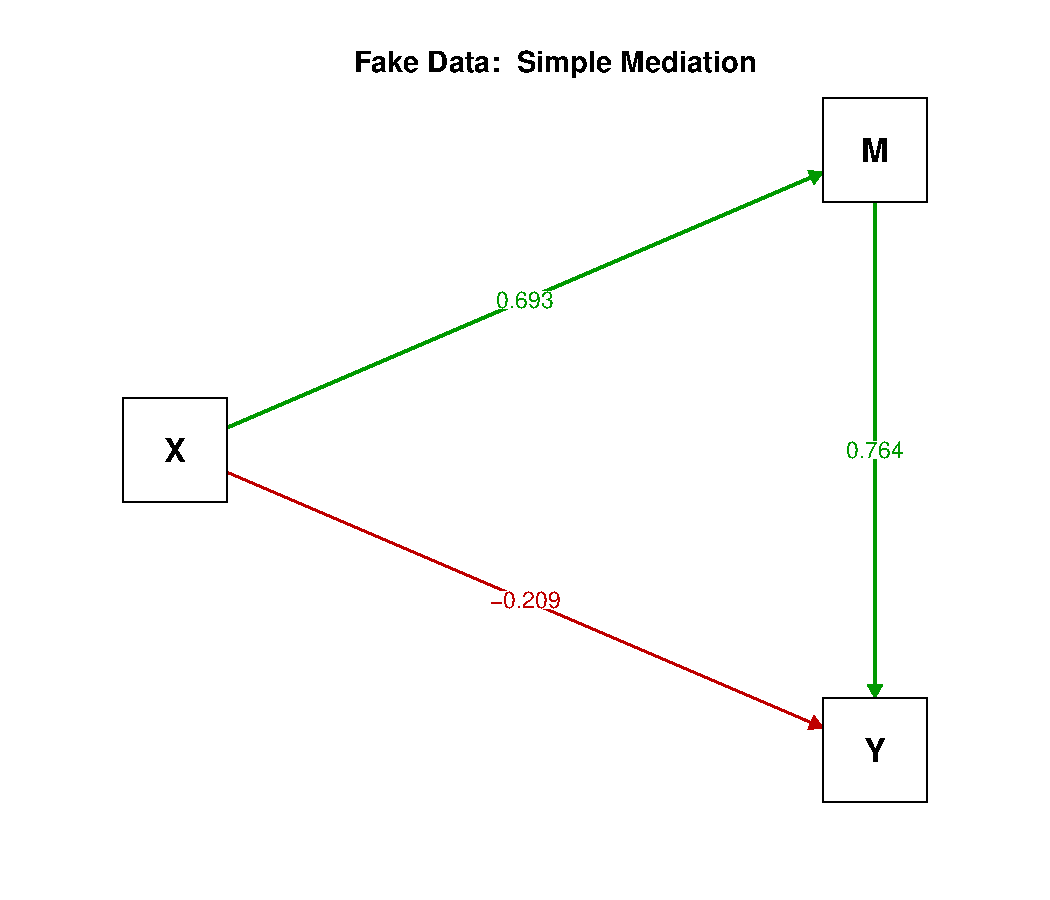
\includegraphics{05-SimpleMed_files/figure-latex/FakyDaty Simple Plot-1.pdf}

Hayes has great examples of APA style tables. I haven't yet found a package that will turn this output into a journal-ready table, however the \emph{semTable} package can at least write the output to a .csv file and you can further manipulate it into a table.

\begin{Shaded}
\begin{Highlighting}[]
\FunctionTok{library}\NormalTok{(semTable)}
\NormalTok{fitTab1 }\OtherTok{\textless{}{-}} \FunctionTok{semTable}\NormalTok{(fit, }\AttributeTok{columns =} \FunctionTok{c}\NormalTok{(}\StringTok{"est"}\NormalTok{, }\StringTok{"se"}\NormalTok{, }\StringTok{"p"}\NormalTok{, }\StringTok{"rsquare"}\NormalTok{),  }\AttributeTok{columnLabels =} \FunctionTok{c}\NormalTok{(}\AttributeTok{eststars =} \StringTok{"Estimate"}\NormalTok{), }\AttributeTok{paramSets =} \FunctionTok{c}\NormalTok{(}\StringTok{"composites"}\NormalTok{, }\StringTok{"loadings"}\NormalTok{, }\StringTok{"slopes"}\NormalTok{, }\StringTok{"intercepts"}\NormalTok{, }\StringTok{"residualvariances"}\NormalTok{), }\AttributeTok{file =} \StringTok{"fitTABLE"}\NormalTok{, }\AttributeTok{type =} \StringTok{"csv"}\NormalTok{, }\AttributeTok{print.results =} \ConstantTok{TRUE}\NormalTok{)}
\end{Highlighting}
\end{Shaded}

\hypertarget{results-4}{%
\subsection{Results}\label{results-4}}

A simple mediation model examined the degree to which M mediated the relation of X on Y. Using the \emph{lavaan} package (v 0.6-7) in R, coefficients for each path, the indirect effect, and total effects were calculated. These values are presented in Table 1 and illustrated in Figure 1. Results suggested that of the variance in M and of the variance in Y were accounted for in the model. The indirect effect (\(B\) = 0.529, \(p\) = 0.000) was statistically significant; the direct effect (\(B\) = -0.209, \(p\) = 0.058) was not. Comparing the nonsignificant direct effect to the statistically significant total effect (\(B\) = 0.321, \(p\) = 0.008) is consistent with the notion that the effect of X on Y is explained through M.

\hypertarget{research-vignette-4}{%
\section{Research Vignette}\label{research-vignette-4}}

The research vignette comes from the Kim, Kendall, and Cheon's \citeyearpar{kim_racial_2017}, ``Racial Microaggressions, Cultural Mistrust, and Mental Health Outcomes Among Asian American College Students.'' Participants were 156 Asian American undergraduate students in the Pacific Northwest. The researchers posited the a priori hypothesis that cultural mistrust would mediate the relationship between racial microaggressions and two sets of outcomes: mental health (e.g., depression, anxiety, well-being) and help-seeking.

Variables used in the study included:

\begin{itemize}
\tightlist
\item
  \textbf{REMS}: Racial and Ethnic Microaggressions Scale (Nadal, 2011). The scale includes 45 items on a 2-point scale where 0 indicates no experience of a microaggressive event and 1 indicates it was experienced at least once within the past six months. Higher scores indicate more experience of microaggressions.
\item
  \textbf{CMI}: Cultural Mistrust Inventory (Terrell \& Terrell, 1981). This scale was adapted to assess cultural mistrust harbored among Asian Americans toward individuals from the mainstream U.S. culture (e.g., Whites). The CMI includes 47 items on a 7-point scale where higher scores indicate a higher degree of cultural mistrust.
\item
  \textbf{ANX}, \textbf{DEP}, \textbf{PWB}: Subscales of the Mental Health Inventory (Veit \& Ware, 1983) that assess the mental health outcomes of anxiety (9 items), depression (4 items), and psychological well-being (14 items). Higher scores (on a 6 point scale) indicate stronger endorsement of the mental health outcome being assessed.
\item
  \textbf{HlpSkg}: The Attiudes Toward Seeking Professional Psychological Help -- Short Form (Fischer \& Farina, 1995) includes 10 items on a 4-point scale (0 = disagree, 3 = agree) where higher scores indicate more favorable attitudes toward help seeking.
\end{itemize}

\hypertarget{simulate-data-from-the-journal-article}{%
\subsection{Simulate Data from the Journal Article}\label{simulate-data-from-the-journal-article}}

First, we simulate the data from the means, standard deviations, and correlation matrix from the journal article.

\begin{Shaded}
\begin{Highlighting}[]
\CommentTok{\#Entering the intercorrelations, means, and standard deviations from the journal article}
\NormalTok{mu }\OtherTok{\textless{}{-}} \FunctionTok{c}\NormalTok{(.}\DecValTok{34}\NormalTok{, }\FloatTok{3.00}\NormalTok{, }\FloatTok{2.98}\NormalTok{, }\FloatTok{2.36}\NormalTok{, }\FloatTok{3.50}\NormalTok{, }\FloatTok{1.64}\NormalTok{)}
\NormalTok{sd }\OtherTok{\textless{}{-}} \FunctionTok{c}\NormalTok{(.}\DecValTok{16}\NormalTok{, .}\DecValTok{83}\NormalTok{, .}\DecValTok{99}\NormalTok{, .}\DecValTok{90}\NormalTok{, .}\DecValTok{90}\NormalTok{, .}\DecValTok{53}\NormalTok{)}
\NormalTok{r\_mat }\OtherTok{\textless{}{-}} \FunctionTok{matrix}\NormalTok{ (}\FunctionTok{c}\NormalTok{(}\DecValTok{1}\NormalTok{,   .}\DecValTok{59}\NormalTok{, .}\DecValTok{26}\NormalTok{,   .}\DecValTok{34}\NormalTok{,  }\SpecialCharTok{{-}}\NormalTok{.}\DecValTok{25}\NormalTok{, }\SpecialCharTok{{-}}\NormalTok{.}\DecValTok{02}\NormalTok{,}
\NormalTok{                  .}\DecValTok{59}\NormalTok{, }\FloatTok{1.00}\NormalTok{, .}\DecValTok{12}\NormalTok{,   .}\DecValTok{19}\NormalTok{,  }\SpecialCharTok{{-}}\NormalTok{.}\DecValTok{28}\NormalTok{, .}\DecValTok{00}\NormalTok{, }
\NormalTok{                  .}\DecValTok{26}\NormalTok{,  .}\DecValTok{12}\NormalTok{, }\FloatTok{1.00}\NormalTok{, .}\DecValTok{66}\NormalTok{,  }\SpecialCharTok{{-}}\NormalTok{.}\DecValTok{55}\NormalTok{, .}\DecValTok{07}\NormalTok{,}
\NormalTok{                  .}\DecValTok{34}\NormalTok{,  .}\DecValTok{19}\NormalTok{, .}\DecValTok{66}\NormalTok{,  }\FloatTok{1.00}\NormalTok{, }\SpecialCharTok{{-}}\NormalTok{.}\DecValTok{66}\NormalTok{, .}\DecValTok{05}\NormalTok{,}
                 \SpecialCharTok{{-}}\NormalTok{.}\DecValTok{25}\NormalTok{, }\SpecialCharTok{{-}}\NormalTok{.}\DecValTok{28}\NormalTok{, }\SpecialCharTok{{-}}\NormalTok{.}\DecValTok{55}\NormalTok{,}\SpecialCharTok{{-}}\NormalTok{.}\DecValTok{66}\NormalTok{,  }\FloatTok{1.00}\NormalTok{, .}\DecValTok{08}\NormalTok{, }
                 \SpecialCharTok{{-}}\NormalTok{.}\DecValTok{02}\NormalTok{,  .}\DecValTok{00}\NormalTok{,  .}\DecValTok{07}\NormalTok{, .}\DecValTok{05}\NormalTok{, .}\DecValTok{08}\NormalTok{,  }\DecValTok{1}\NormalTok{), }\AttributeTok{ncol =} \DecValTok{6}\NormalTok{)}
\CommentTok{\#Creating a covariance matrix}
\NormalTok{cov\_mat }\OtherTok{\textless{}{-}}\NormalTok{ sd }\SpecialCharTok{\%*\%} \FunctionTok{t}\NormalTok{(sd) }\SpecialCharTok{*}\NormalTok{ r\_mat}

\CommentTok{\#Set random seed so that the following matrix always gets the same results.}
\FunctionTok{set.seed}\NormalTok{(}\DecValTok{210409}\NormalTok{)}
\FunctionTok{library}\NormalTok{(MASS)}
\end{Highlighting}
\end{Shaded}

\begin{verbatim}
## 
## Attaching package: 'MASS'
\end{verbatim}

\begin{verbatim}
## The following object is masked from 'package:formattable':
## 
##     area
\end{verbatim}

\begin{Shaded}
\begin{Highlighting}[]
\NormalTok{Kim\_df }\OtherTok{\textless{}{-}} \FunctionTok{mvrnorm}\NormalTok{(}\AttributeTok{n =} \DecValTok{156}\NormalTok{, }\AttributeTok{mu=}\NormalTok{mu, }\AttributeTok{Sigma =}\NormalTok{ cov\_mat, }\AttributeTok{empirical =} \ConstantTok{TRUE}\NormalTok{)}
\FunctionTok{colMeans}\NormalTok{(Kim\_df)}
\end{Highlighting}
\end{Shaded}

\begin{verbatim}
## [1] 0.34 3.00 2.98 2.36 3.50 1.64
\end{verbatim}

\begin{Shaded}
\begin{Highlighting}[]
\CommentTok{\#Checking our work against the original correlation matrix}
\FunctionTok{round}\NormalTok{(}\FunctionTok{cor}\NormalTok{(Kim\_df),}\DecValTok{3}\NormalTok{)}
\end{Highlighting}
\end{Shaded}

\begin{verbatim}
##       [,1]  [,2]  [,3]  [,4]  [,5]  [,6]
## [1,]  1.00  0.59  0.26  0.34 -0.25 -0.02
## [2,]  0.59  1.00  0.12  0.19 -0.28  0.00
## [3,]  0.26  0.12  1.00  0.66 -0.55  0.07
## [4,]  0.34  0.19  0.66  1.00 -0.66  0.05
## [5,] -0.25 -0.28 -0.55 -0.66  1.00  0.08
## [6,] -0.02  0.00  0.07  0.05  0.08  1.00
\end{verbatim}

\begin{Shaded}
\begin{Highlighting}[]
\CommentTok{\#renaming the variables}
\FunctionTok{as.data.frame}\NormalTok{(Kim\_df, }\AttributeTok{row.names =} \ConstantTok{NULL}\NormalTok{, }\AttributeTok{optional =} \ConstantTok{FALSE}\NormalTok{, }\AttributeTok{make.names =} \ConstantTok{TRUE}\NormalTok{)}
\end{Highlighting}
\end{Shaded}

\begin{verbatim}
##              V1        V2        V3         V4       V5        V6
## 1    0.31480075 3.7742194 3.9885237  2.6561280 3.902766 1.2282205
## 2    0.12504376 2.4630397 3.1591179  1.7873208 4.434146 1.4990282
## 3    0.17784660 1.8376841 3.8176890  2.5481372 3.299962 1.3126023
## 4    0.75415493 4.8268167 3.2961255  2.1700517 3.274046 1.4857932
## 5    0.28473851 2.1622754 2.9837665  2.6213814 3.851441 1.4330810
## 6    0.37498180 4.1070853 3.4324724  3.0951215 2.880348 1.9417795
## 7    0.17693663 1.8937966 3.6027771  2.7026733 4.159506 1.5721610
## 8    0.29125231 2.6160275 2.9306768  2.0874299 4.148450 2.4368026
## 9    0.20511465 2.7325373 2.7857356  1.9796662 3.253885 1.8116435
## 10   0.53359317 3.2392905 3.0132959  2.0895764 4.367763 2.4243275
## 11   0.63114162 3.9771384 3.4587058  2.9438475 1.807563 1.2569630
## 12   0.40896721 3.6662876 4.0138230  3.3097403 2.742602 1.7651180
## 13   0.26224312 2.8483570 4.2526175  2.8099626 3.295733 1.9924000
## 14   0.32704221 3.1617904 3.1070588  2.4118363 3.810240 2.3476934
## 15   0.60748029 3.6350970 3.9352681  3.2005377 3.393395 1.7029545
## 16   0.55843862 3.7676612 2.6728071  1.8013062 2.456926 1.8749401
## 17   0.16189032 2.7778703 2.1929777  3.1968281 4.053990 1.4759460
## 18   0.09036787 2.5826597 1.7540157  1.4921435 3.472623 1.5609561
## 19   0.60989051 4.6660979 3.4085289  2.2633219 2.865315 1.3588810
## 20   0.45105455 2.5689387 3.5198695  3.5398776 2.862075 2.1906123
## 21   0.08222908 2.8395169 1.7860559  1.0991829 4.203118 1.5276039
## 22   0.24533439 1.5002846 4.7377924  4.0310332 1.560094 1.7210027
## 23   0.38076827 3.0562669 1.6113009  1.0246868 4.530600 0.9667363
## 24   0.20535295 2.9163293 4.1163801  3.3911153 2.241094 2.5286007
## 25   0.41877232 2.7303151 1.5616356  2.4506453 3.626496 1.3331132
## 26   0.26617565 3.2712843 3.1396021  2.5046344 3.107293 2.6373851
## 27   0.28769261 3.9226886 2.0225615  2.5273085 2.897739 1.4673821
## 28   0.39977557 2.9378013 4.5977776  2.2221782 2.777697 1.5796865
## 29   0.56682075 3.2977619 4.1540235  1.4287847 3.676300 2.6380399
## 30   0.52963158 3.4581461 3.8075875  2.7607609 3.345936 1.3725315
## 31   0.22833829 2.9526622 2.8162920  1.8302324 4.461217 1.6180715
## 32   0.20715467 2.6428462 0.6872940  0.6175158 5.945886 1.2083258
## 33   0.41239292 2.9599932 2.6683891  2.5953392 4.100208 1.7439009
## 34   0.17706607 1.9297199 1.6580187  1.4474162 3.547635 0.9385664
## 35   0.44076050 3.7674252 0.6451316  0.9195607 4.872259 2.9042943
## 36   0.31629873 2.1146493 3.7536880  3.0360594 2.838068 1.0597817
## 37   0.37035488 3.8020496 2.7486592  0.2643106 4.290151 1.7539316
## 38   0.18525000 2.7299318 1.3546404 -0.2523240 4.721493 1.2751736
## 39   0.50115577 3.1349456 3.2421449  3.6172850 2.243026 1.7142033
## 40   0.46397513 3.0130363 1.6878921  2.1082437 3.980620 1.8878141
## 41   0.35589931 3.8035799 2.6925134  2.7952193 2.433082 1.7502752
## 42   0.44021737 2.9537302 2.5509321  2.1958486 4.282946 1.6619111
## 43   0.32847707 2.7533998 2.1885928  2.1955374 4.179124 1.2966225
## 44   0.56599738 3.8086684 2.6614906  1.7883525 3.534684 0.9109111
## 45   0.63298561 5.4722538 2.6246473  2.0323609 4.245740 1.6019083
## 46   0.36671192 3.8373379 1.2029473  1.0808787 4.120857 1.4083544
## 47   0.65026343 4.4611344 3.3155709  3.2096415 3.275165 1.8197487
## 48   0.21525053 1.4784055 0.6087000  1.5537867 3.773753 1.6499578
## 49   0.27368491 1.1111501 1.2805981  1.9063158 4.896829 0.9122461
## 50   0.10696105 1.8148086 3.8605081  2.9060923 3.723161 2.1977074
## 51   0.33966450 3.4810637 3.1089231  3.2156230 2.771850 1.6027278
## 52   0.57280640 3.1872778 3.0340553  2.9384369 3.690575 1.7279573
## 53   0.15508574 2.1099147 2.3821604  2.0299025 3.666993 1.8155390
## 54   0.40500505 2.5808052 3.8734464  2.9063157 3.539234 1.6241724
## 55   0.12820991 2.1598440 3.3058396  2.2974267 3.559505 2.0272936
## 56   0.33136509 3.5787209 0.5054556  1.3450229 3.588936 2.6649975
## 57   0.37281298 1.9809393 2.4679268  2.0532096 2.693133 1.8264299
## 58   0.54951382 2.5396186 1.9478418  1.9405555 3.707789 1.2143895
## 59   0.42571472 3.8397686 3.4512906  2.5756583 2.748384 1.0366664
## 60   0.45118332 2.6936624 4.3733104  2.6169130 2.954446 0.4413846
## 61   0.53225789 2.6442805 4.3567514  2.7931458 3.160311 2.5012683
## 62   0.32424735 3.6281840 3.6375053  1.7813392 3.975108 1.1801099
## 63   0.56918841 3.2878176 2.3571347  1.9000358 3.707492 1.5158290
## 64   0.39689825 2.8722661 3.3891630  3.6161698 4.068442 1.9059061
## 65   0.50916945 3.0716802 3.0138930  3.3409739 3.174682 1.9282731
## 66   0.37381045 2.8613972 2.5346525  2.1169429 4.467001 1.1984569
## 67   0.44510070 3.4257946 3.1816739  2.7318242 3.732238 1.6831477
## 68   0.39299460 3.2010693 3.0060414  2.7628540 3.740873 2.4609643
## 69   0.44653298 3.1644675 3.6843226  3.1614193 3.279748 0.8922136
## 70   0.21899834 3.1967184 3.2764076  2.6424565 2.771732 2.2746857
## 71   0.25699825 4.2762230 3.7504485  2.6255869 3.432270 1.9718086
## 72   0.40767690 3.9634931 1.7851558  2.0298828 4.034073 0.8764307
## 73   0.47161399 3.3279451 5.5579604  3.6499364 2.663229 1.9991762
## 74   0.16250469 3.2773109 2.3015365  2.7213271 2.207900 0.6357077
## 75   0.21824252 1.9657893 3.6326756  2.3072120 3.714804 1.7842104
## 76   0.35899955 4.7632581 2.7294744  1.6372696 3.315482 1.7298316
## 77   0.27873590 3.7828931 3.4194274  2.6702150 3.061570 2.5602023
## 78   0.32614924 2.4435997 3.0606050  1.7580998 4.515989 1.0150848
## 79   0.44731840 2.6447258 2.4664493  3.3599532 3.161522 1.8540898
## 80   0.38029332 2.8780152 2.5960868  2.4639264 4.166040 1.5279508
## 81   0.29347514 2.0532644 2.5949659  2.3422173 4.566912 1.7580519
## 82   0.33449008 1.6763340 4.0745945  2.4576674 1.670886 0.3301944
## 83  -0.13333427 1.8646838 1.8605537  0.8743076 3.859640 1.2873846
## 84   0.35487008 3.1329063 5.1607506  4.4201740 3.263059 1.5195622
## 85   0.58713616 3.5871929 3.5483750  4.3854551 2.030597 0.9455332
## 86   0.45786163 3.1040782 5.0810000  2.4448840 2.710524 1.1693378
## 87   0.11330940 2.7322124 2.9335807  2.6275255 4.450236 2.6072942
## 88   0.44777502 3.9562751 2.8594018  1.2333628 5.032948 2.1101670
## 89   0.20234249 3.5441251 1.4882324  0.3852576 4.367248 0.4775579
## 90   0.34962746 3.0855190 2.6132050  3.0958749 3.614912 2.4456362
## 91   0.35472400 1.3014022 2.6016511  1.1155728 4.948843 1.1118416
## 92   0.23522461 2.2139784 2.9370279  2.1549473 4.138606 1.7861832
## 93   0.42014755 4.1320485 2.7372095  1.4261881 2.536445 0.7664355
## 94   0.15876267 3.2073345 1.5006009  0.2652437 4.404531 1.3220635
## 95  -0.09879649 0.8656131 2.7234710  0.6494040 5.941681 2.7164183
## 96   0.38591913 4.9543775 3.8013379  2.7004684 2.425454 1.7873045
## 97   0.44230619 3.2033360 4.2147040  3.6971513 2.430067 1.4020194
## 98   0.29716688 2.3867630 2.9367032  2.4687254 4.053484 1.4651382
## 99   0.25872796 2.2176660 1.2114582  1.1411757 4.777005 1.5079464
## 100  0.06517719 2.7807617 3.4760948  2.0910964 4.221674 2.1545484
## 101  0.16162849 3.8400098 1.7971752  2.4634779 2.940266 1.0140635
## 102  0.64606063 4.3452532 4.0757378  4.4425493 2.503920 1.4400385
## 103  0.43953190 2.6128498 2.7762497  2.4062207 3.726635 0.2829370
## 104  0.32010790 3.0664919 2.4460013  2.0391555 3.790884 0.8317398
## 105  0.23294638 2.8678142 3.3969138  3.1130449 2.096275 1.6124933
## 106  0.50169163 3.1905757 3.6799971  3.4794417 2.458951 1.5971075
## 107  0.29363188 2.6876792 2.9182203  2.2699264 1.957908 2.5447356
## 108  0.26214714 3.4488353 3.8895770  2.8992699 2.788475 1.6974445
## 109  0.37009802 3.7469694 2.9289129  2.9753900 2.931447 1.8848354
## 110  0.29730729 3.1534935 3.3337636  3.0937892 2.581927 2.3980973
## 111  0.24470529 3.2782295 2.8703885  2.2915569 3.751316 1.5109690
## 112  0.54659869 3.9875404 4.8961430  4.0922097 1.973596 1.2552789
## 113  0.10697366 1.7824763 1.9450107  2.5996601 4.482268 2.2628556
## 114  0.26811871 2.5759431 2.8436596  0.8909314 3.820002 1.0753586
## 115  0.43803765 2.4273121 3.3702456  2.6467107 4.705230 2.7045322
## 116 -0.06773831 1.0890615 2.1039908  1.6805607 3.898468 1.4121238
## 117  0.67609125 3.4169175 3.0278088  2.4529501 3.759270 2.6841150
## 118  0.22489645 3.3639686 4.2235025  3.4781409 2.397229 1.2734251
## 119  0.48300880 2.7120258 3.2456654  2.1793229 3.866140 2.4408081
## 120  0.21667980 3.0603200 0.7108609  1.4644661 5.260412 1.9287701
## 121  0.06512801 1.5886292 2.3749889  0.9180135 4.825579 1.5245304
## 122  0.61003798 3.6223559 2.4047411  2.1696687 2.872875 1.8673206
## 123  0.22977532 3.0189730 2.4342990  2.1243346 3.603260 1.0869989
## 124  0.36422147 2.7425189 3.1556307  1.5394070 4.365395 2.0480712
## 125  0.22933372 2.2046979 2.6570211  2.8655072 2.491654 1.0139864
## 126  0.43238708 4.3102068 1.4277537  1.8567860 3.762495 1.5152676
## 127  0.38990877 2.7218866 2.2477225  1.0646075 4.641716 1.0071908
## 128  0.21753221 1.5882455 1.7407732  1.8213958 3.979175 2.0259607
## 129  0.24771023 1.8672735 2.1881830  1.7507315 4.963161 1.0898960
## 130  0.75408295 4.1289706 3.5474464  3.7791487 2.890496 1.5877356
## 131  0.41644783 2.3299547 3.2208705  2.4181467 4.168489 2.0548755
## 132  0.51769871 4.8743013 3.0157732  3.4737052 3.199802 1.1111757
## 133  0.35717215 2.5981651 2.8779430  2.8980202 3.187424 1.7153314
## 134  0.26920553 3.6847735 3.5523502  2.1903271 2.951610 1.5712546
## 135  0.16434131 1.2258814 3.0293592  1.9656563 3.951977 1.6376233
## 136  0.31628364 2.9034206 1.6436139  1.1249672 4.345822 2.1125579
## 137  0.43040767 3.5183625 3.1331817  1.5718843 3.896956 0.9777469
## 138  0.09448973 1.9683952 2.4498808  1.8165286 3.656073 1.3069823
## 139  0.35002893 3.5852879 2.5912530  1.6491977 5.409283 1.5340238
## 140  0.42296660 3.0640201 3.3574675  2.0421916 3.569581 0.8512156
## 141  0.24932068 3.4213164 2.7485416  3.6280473 2.312726 1.2516653
## 142  0.53062494 3.6640311 5.0907192  4.5694108 1.350203 1.8851816
## 143  0.27962118 3.3932218 2.7264126  1.6711386 3.765364 2.2954985
## 144  0.23322586 3.3279561 3.1592797  1.8154681 1.526867 2.0054852
## 145  0.37962928 2.9616314 3.0021556  2.2003911 3.365035 1.6114163
## 146  0.58980078 3.4742094 4.9949216  3.5702922 1.845780 1.9212095
## 147  0.19270590 2.2602334 2.8233585  0.9669035 4.679490 2.3836889
## 148  0.31012390 2.1745958 4.0843806  3.6022376 3.523946 1.6006189
## 149  0.32504460 3.3473480 2.5347074  2.3469577 3.709119 1.5668096
## 150  0.15226205 2.0648724 5.0295232  2.4532674 2.093509 2.0246498
## 151  0.28115818 1.9376116 3.6657196  2.5134560 2.871831 1.2246409
## 152  0.31936688 3.2432213 4.9907982  2.7616598 4.100608 1.8425462
## 153  0.26239276 3.3908566 2.7704343  2.4932497 2.810725 2.4545378
## 154  0.18193724 3.1099861 2.9947179  3.4509396 2.180071 1.4960772
## 155  0.24134651 2.5263768 2.2951753  1.7940080 3.185113 1.7917425
## 156  0.22502241 2.8972357 4.7873242  4.3623474 1.775025 1.0875423
\end{verbatim}

\begin{Shaded}
\begin{Highlighting}[]
\FunctionTok{library}\NormalTok{(tidyverse)}
\end{Highlighting}
\end{Shaded}

\begin{verbatim}
## -- Attaching core tidyverse packages ------------------------ tidyverse 2.0.0 --
## v dplyr     1.1.2     v readr     2.1.4
## v forcats   1.0.0     v stringr   1.5.0
## v ggplot2   3.4.3     v tibble    3.2.1
## v lubridate 1.9.2     v tidyr     1.3.0
## v purrr     1.0.1     
## -- Conflicts ------------------------------------------ tidyverse_conflicts() --
## x ggplot2::%+%()   masks psych::%+%()
## x ggplot2::alpha() masks psych::alpha()
## x dplyr::filter()  masks stats::filter()
## x dplyr::lag()     masks stats::lag()
## x dplyr::select()  masks MASS::select()
## i Use the conflicted package (<http://conflicted.r-lib.org/>) to force all conflicts to become errors
\end{verbatim}

\begin{Shaded}
\begin{Highlighting}[]
\NormalTok{Kim\_df }\OtherTok{\textless{}{-}}\NormalTok{ Kim\_df}\SpecialCharTok{\%\textgreater{}\%}
\NormalTok{  as.data.frame }\SpecialCharTok{\%\textgreater{}\%}
  \FunctionTok{rename}\NormalTok{(}\AttributeTok{REMS =}\NormalTok{ V1, }\AttributeTok{CMI =}\NormalTok{ V2, }\AttributeTok{ANX =}\NormalTok{ V3, }\AttributeTok{DEP =}\NormalTok{ V4, }\AttributeTok{PWB =}\NormalTok{ V5, }\AttributeTok{HlpSk =}\NormalTok{ V6)}
\end{Highlighting}
\end{Shaded}

\begin{Shaded}
\begin{Highlighting}[]
\CommentTok{\#look at the first 6 rows of the new df}
\FunctionTok{head}\NormalTok{(Kim\_df)}
\end{Highlighting}
\end{Shaded}

\begin{verbatim}
##        REMS      CMI      ANX      DEP      PWB    HlpSk
## 1 0.3148008 3.774219 3.988524 2.656128 3.902766 1.228220
## 2 0.1250438 2.463040 3.159118 1.787321 4.434146 1.499028
## 3 0.1778466 1.837684 3.817689 2.548137 3.299962 1.312602
## 4 0.7541549 4.826817 3.296125 2.170052 3.274046 1.485793
## 5 0.2847385 2.162275 2.983767 2.621381 3.851441 1.433081
## 6 0.3749818 4.107085 3.432472 3.095121 2.880348 1.941779
\end{verbatim}

Let's check the descriptives to see if they align with those in the article.

\begin{Shaded}
\begin{Highlighting}[]
\FunctionTok{library}\NormalTok{(psych)}
\NormalTok{psych}\SpecialCharTok{::}\FunctionTok{describe}\NormalTok{(Kim\_df)}
\end{Highlighting}
\end{Shaded}

\begin{verbatim}
##       vars   n mean   sd median trimmed  mad   min  max range  skew kurtosis
## REMS     1 156 0.34 0.16   0.33    0.34 0.16 -0.13 0.75  0.89  0.03     0.16
## CMI      2 156 3.00 0.83   3.06    3.00 0.72  0.87 5.47  4.61  0.01     0.13
## ANX      3 156 2.98 0.99   2.99    2.98 0.83  0.51 5.56  5.05 -0.02     0.12
## DEP      4 156 2.36 0.90   2.41    2.36 0.83 -0.25 4.57  4.82 -0.05     0.10
## PWB      5 156 3.50 0.90   3.61    3.51 0.97  1.35 5.95  4.60 -0.04    -0.23
## HlpSk    6 156 1.64 0.53   1.61    1.63 0.49  0.28 2.90  2.62  0.07    -0.24
##         se
## REMS  0.01
## CMI   0.07
## ANX   0.08
## DEP   0.07
## PWB   0.07
## HlpSk 0.04
\end{verbatim}

There are a number of reasons I love the Kim et al. \citeyearpar{kim_racial_2017} manuscript. One is that their approach was openly one that tested \emph{alternate models}. Byrne \citeyearpar{byrne_structural_2016} credits Joreskog \citep{bollen_testing_1993} with classifying the researcher's model testing approach in three ways. If someone is \emph{strictly confirmatory}, they only test the model they proposed and then accept or reject it without further alteration. While this is the tradition of null hypothesis significance testing, it contributes to the ``file drawer problem'' of unpublished, non-significant, findings. Additionally, the data are them discarded -- potentially losing valuable resource. The \emph{alternative models} approach is to propose a handful of competing models before beginning the analysis and then evaluating to see if one model is superior to the other. The third option is \emph{model generating}. In this case the researcher begins with a theoretically proposed model. In the presence of poor fit, the researcher seeks to identify the source of misfit -- respecifying it to best represent the sample data. The researcher must use caution to produce a model that fits well and is meaningful.

Several of the Kim et al. \citeyearpar{kim_racial_2017} models were non-significant. To demonstrate a model that is statistically significant, I will test the hypothesis that racial microaggressions (REMS, the X variable) influence depression (DEP, the Y variable) through cultural mistrust (CMI, the M variable).

\begin{figure}
\centering
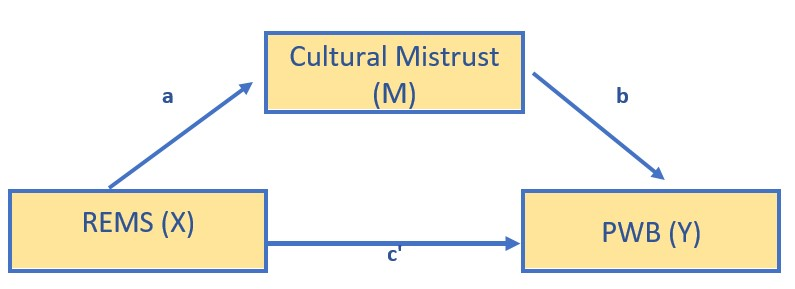
\includegraphics{images/SimpleMed/Kim_SimpMed.jpg}
\caption{Image of the simple mediation model from Kim et al.}
\end{figure}

\hypertarget{specify-the-model-in-lavaan}{%
\subsection{\texorpdfstring{Specify the Model in \emph{lavaan}}{Specify the Model in lavaan}}\label{specify-the-model-in-lavaan}}

I am a big fan of ``copying the model.'' In specifying my model I used our simple mediation template above

\begin{itemize}
\tightlist
\item
  replaced the Y, X, and M with variables names
\item
  replacing the name of the df
\item
  updated the object names (so I could use them in the same .rmd file)
\end{itemize}

\begin{Shaded}
\begin{Highlighting}[]
\FunctionTok{library}\NormalTok{(lavaan)}
\FunctionTok{set.seed}\NormalTok{(}\DecValTok{210410}\NormalTok{) }\CommentTok{\#reset in case you choose to separate these sections}
\NormalTok{Kim\_model }\OtherTok{\textless{}{-}} \StringTok{\textquotesingle{}}
\StringTok{          PWB \textasciitilde{} b*CMI + c\_p*REMS }
\StringTok{          CMI \textasciitilde{}a*REMS}
\StringTok{          }
\StringTok{          indirect :=  a*b}
\StringTok{          direct  := c\_p}
\StringTok{          total\_c  := c\_p + (a*b)}
\StringTok{          \textquotesingle{}}
\end{Highlighting}
\end{Shaded}

\begin{Shaded}
\begin{Highlighting}[]
\NormalTok{Kim\_fit }\OtherTok{\textless{}{-}} \FunctionTok{sem}\NormalTok{(Kim\_model, }\AttributeTok{data =}\NormalTok{ Kim\_df, }\AttributeTok{se=}\StringTok{"bootstrap"}\NormalTok{, }\AttributeTok{missing=} \StringTok{\textquotesingle{}fiml\textquotesingle{}}\NormalTok{)}
\end{Highlighting}
\end{Shaded}

\begin{Shaded}
\begin{Highlighting}[]
\NormalTok{Kim\_summary }\OtherTok{\textless{}{-}} \FunctionTok{summary}\NormalTok{(Kim\_fit, }\AttributeTok{standardized=}\NormalTok{T, }\AttributeTok{rsq=}\NormalTok{T, }\AttributeTok{fit=}\ConstantTok{TRUE}\NormalTok{, }\AttributeTok{ci=}\ConstantTok{TRUE}\NormalTok{)}
\NormalTok{Kim\_ParamEsts }\OtherTok{\textless{}{-}} \FunctionTok{parameterEstimates}\NormalTok{(Kim\_fit, }\AttributeTok{boot.ci.type =} \StringTok{"bca.simple"}\NormalTok{, }\AttributeTok{standardized=}\ConstantTok{TRUE}\NormalTok{)}
\NormalTok{Kim\_summary}
\end{Highlighting}
\end{Shaded}

\begin{verbatim}
## lavaan 0.6.16 ended normally after 1 iteration
## 
##   Estimator                                         ML
##   Optimization method                           NLMINB
##   Number of model parameters                         7
## 
##   Number of observations                           156
##   Number of missing patterns                         1
## 
## Model Test User Model:
##                                                       
##   Test statistic                                 0.000
##   Degrees of freedom                                 0
## 
## Model Test Baseline Model:
## 
##   Test statistic                                81.362
##   Degrees of freedom                                 3
##   P-value                                        0.000
## 
## User Model versus Baseline Model:
## 
##   Comparative Fit Index (CFI)                    1.000
##   Tucker-Lewis Index (TLI)                       1.000
##                                                       
##   Robust Comparative Fit Index (CFI)             1.000
##   Robust Tucker-Lewis Index (TLI)                1.000
## 
## Loglikelihood and Information Criteria:
## 
##   Loglikelihood user model (H0)               -355.521
##   Loglikelihood unrestricted model (H1)       -355.521
##                                                       
##   Akaike (AIC)                                 725.042
##   Bayesian (BIC)                               746.391
##   Sample-size adjusted Bayesian (SABIC)        724.234
## 
## Root Mean Square Error of Approximation:
## 
##   RMSEA                                          0.000
##   90 Percent confidence interval - lower         0.000
##   90 Percent confidence interval - upper         0.000
##   P-value H_0: RMSEA <= 0.050                       NA
##   P-value H_0: RMSEA >= 0.080                       NA
##                                                       
##   Robust RMSEA                                   0.000
##   90 Percent confidence interval - lower         0.000
##   90 Percent confidence interval - upper         0.000
##   P-value H_0: Robust RMSEA <= 0.050                NA
##   P-value H_0: Robust RMSEA >= 0.080                NA
## 
## Standardized Root Mean Square Residual:
## 
##   SRMR                                           0.000
## 
## Parameter Estimates:
## 
##   Standard errors                            Bootstrap
##   Number of requested bootstrap draws             1000
##   Number of successful bootstrap draws            1000
## 
## Regressions:
##                    Estimate  Std.Err  z-value  P(>|z|) ci.lower ci.upper
##   PWB ~                                                                 
##     CMI        (b)   -0.220    0.108   -2.046    0.041   -0.423   -0.006
##     REMS     (c_p)   -0.732    0.513   -1.427    0.154   -1.786    0.270
##   CMI ~                                                                 
##     REMS       (a)    3.061    0.300   10.188    0.000    2.475    3.655
##    Std.lv  Std.all
##                   
##    -0.220   -0.203
##    -0.732   -0.130
##                   
##     3.061    0.590
## 
## Intercepts:
##                    Estimate  Std.Err  z-value  P(>|z|) ci.lower ci.upper
##    .PWB               4.410    0.272   16.220    0.000    3.821    4.910
##    .CMI               1.959    0.118   16.598    0.000    1.717    2.187
##    Std.lv  Std.all
##     4.410    4.916
##     1.959    2.368
## 
## Variances:
##                    Estimate  Std.Err  z-value  P(>|z|) ci.lower ci.upper
##    .PWB               0.733    0.082    8.912    0.000    0.564    0.889
##    .CMI               0.446    0.050    8.979    0.000    0.349    0.549
##    Std.lv  Std.all
##     0.733    0.911
##     0.446    0.652
## 
## R-Square:
##                    Estimate
##     PWB               0.089
##     CMI               0.348
## 
## Defined Parameters:
##                    Estimate  Std.Err  z-value  P(>|z|) ci.lower ci.upper
##     indirect         -0.675    0.330   -2.043    0.041   -1.314   -0.018
##     direct           -0.732    0.513   -1.426    0.154   -1.786    0.270
##     total_c          -1.406    0.421   -3.339    0.001   -2.192   -0.545
##    Std.lv  Std.all
##    -0.675   -0.120
##    -0.732   -0.130
##    -1.406   -0.250
\end{verbatim}

\begin{Shaded}
\begin{Highlighting}[]
\NormalTok{Kim\_ParamEsts}
\end{Highlighting}
\end{Shaded}

\begin{verbatim}
##         lhs op       rhs    label    est    se      z pvalue ci.lower ci.upper
## 1       PWB  ~       CMI        b -0.220 0.108 -2.046  0.041   -0.435   -0.013
## 2       PWB  ~      REMS      c_p -0.732 0.513 -1.427  0.154   -1.852    0.202
## 3       CMI  ~      REMS        a  3.061 0.300 10.188  0.000    2.467    3.643
## 4       PWB ~~       PWB           0.733 0.082  8.912  0.000    0.595    0.935
## 5       CMI ~~       CMI           0.446 0.050  8.979  0.000    0.362    0.564
## 6      REMS ~~      REMS           0.025 0.000     NA     NA    0.025    0.025
## 7       PWB ~1                     4.410 0.272 16.220  0.000    3.880    4.934
## 8       CMI ~1                     1.959 0.118 16.598  0.000    1.703    2.185
## 9      REMS ~1                     0.340 0.000     NA     NA    0.340    0.340
## 10 indirect :=       a*b indirect -0.675 0.330 -2.043  0.041   -1.364   -0.077
## 11   direct :=       c_p   direct -0.732 0.513 -1.426  0.154   -1.852    0.202
## 12  total_c := c_p+(a*b)  total_c -1.406 0.421 -3.339  0.001   -2.263   -0.605
##    std.lv std.all std.nox
## 1  -0.220  -0.203  -0.203
## 2  -0.732  -0.130  -0.816
## 3   3.061   0.590   3.699
## 4   0.733   0.911   0.911
## 5   0.446   0.652   0.652
## 6   0.025   1.000   0.025
## 7   4.410   4.916   4.916
## 8   1.959   2.368   2.368
## 9   0.340   2.132   0.340
## 10 -0.675  -0.120  -0.752
## 11 -0.732  -0.130  -0.816
## 12 -1.406  -0.250  -1.568
\end{verbatim}

\hypertarget{interpret-the-output-1}{%
\subsection{Interpret the Output}\label{interpret-the-output-1}}

\begin{itemize}
\tightlist
\item
  Overall, our model accounted for of the variance in the IV and of the variance in the mediator.
\item
  a path = 3.061, \(p\) = 0.000
\item
  b path = -0.220, \(p\) = 0.041
\item
  the indirect effect is a product of the a and b paths (-0.675); while we don't hand calculate it's significance, we see that it is \(p\) = 0.041; the bias-corrected bootstrapped confidence intervals can sometimes be more lenient than \(p\) values; it is important they don't cross zero. They don't: CI95 -1.364 to -0.077\\
\item
  the direct effect (c', c prime, or c\_p) is the isolated effect of X on Y when including M. We hope this value is LOWER than the total effect because this means that including M shared some of the variance in predicting Y: c' = -0.732, \(p\) = 0.154, and it is no longer signifcant.
\item
  we also see the total effect; this value is
\item
  identical to the value of simply predicting Y on X (with no M it the model)
\item
  the value of a(b) + c\_p: 3.061(-0.220) + -0.732 = -1.406 (\(p\) = 0.001)
\end{itemize}

\hypertarget{a-figure-and-a-table}{%
\subsection{A Figure and a Table}\label{a-figure-and-a-table}}

I make it a practice to immediately plot what I did. Because the plotting packages use our models, this can be a helpful self-check of our work.

\begin{Shaded}
\begin{Highlighting}[]
\FunctionTok{library}\NormalTok{(semPlot)}
\FunctionTok{semPaths}\NormalTok{(Kim\_fit, }\CommentTok{\#must identiy the model you want to map}
         \AttributeTok{what =} \StringTok{"est"}\NormalTok{, }\CommentTok{\#"est" plots the estimates, but keeps it greyscale with no fading}
         \CommentTok{\#whatLabels = "stand", \#"stand" changes to standardized values}
         \AttributeTok{layout =} \StringTok{\textquotesingle{}tree\textquotesingle{}}\NormalTok{, }\AttributeTok{rotation =} \DecValTok{2}\NormalTok{, }\CommentTok{\#together, puts predictors on left, IVs on right }
         \AttributeTok{edge.label.cex =} \FloatTok{1.00}\NormalTok{, }\CommentTok{\#font size of parameter values}
         \CommentTok{\#edge.color = "black", \#overwrites the green/black coloring}
         \AttributeTok{sizeMan=}\DecValTok{10}\NormalTok{, }\CommentTok{\#size of squares/observed/"manifest" variables}
         \AttributeTok{fade=}\ConstantTok{FALSE}\NormalTok{, }\CommentTok{\#if TRUE, there lines are faded such that weaker lines correspond with lower values {-}{-} a cool effect, but tough for journals}
         \AttributeTok{esize=}\DecValTok{2}\NormalTok{, }
         \AttributeTok{asize=}\DecValTok{3}\NormalTok{,}
         \CommentTok{\#label.prop = .5,}
         \AttributeTok{label.font =} \FloatTok{2.5}\NormalTok{, }\CommentTok{\#controls size (I think) of font for labels}
         \AttributeTok{label.scale =} \ConstantTok{TRUE}\NormalTok{, }\CommentTok{\#if false, the labels will not scale to fit inside the nodes}
         \AttributeTok{nDigits =} \DecValTok{3}\NormalTok{, }\CommentTok{\#decimal places (default is 2)}
         \AttributeTok{residuals =} \ConstantTok{FALSE}\NormalTok{,}\CommentTok{\#excludes residuals (and variances) from the path diagram}
         \AttributeTok{nCharNodes =} \DecValTok{0}\NormalTok{, }\CommentTok{\#specifies how many characters to abbreviate variable lables; default is 3.  If 0, uses your entire variable label and adjusts fontsize (which could be a downside)}
         \AttributeTok{intercepts =} \ConstantTok{FALSE}\NormalTok{, }\CommentTok{\#gets rid of those annoying triangles (intercepts) in the path diagram)}
\NormalTok{)}
\FunctionTok{title}\NormalTok{(}\StringTok{"Depression by Racial Microaggressions via Cultural Mistrust"}\NormalTok{)}
\end{Highlighting}
\end{Shaded}

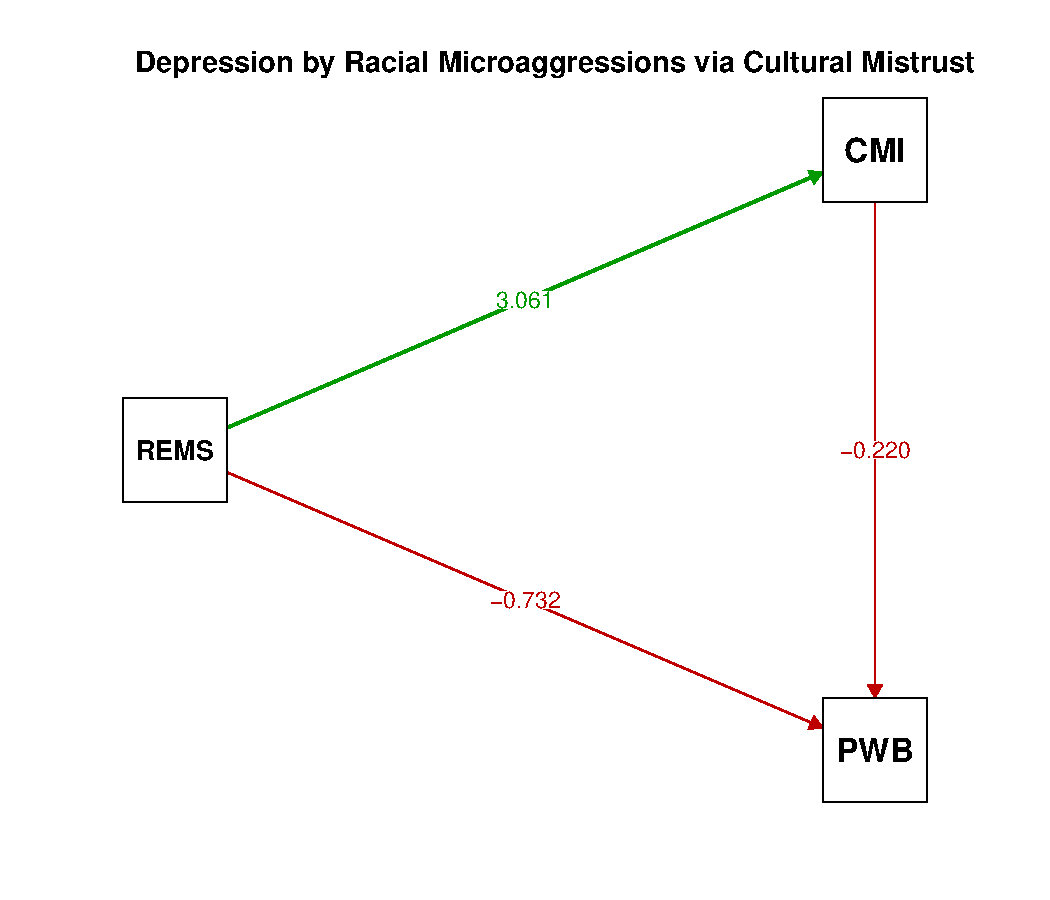
\includegraphics{05-SimpleMed_files/figure-latex/semPLOT of PMI-1.pdf}

The semTable package can be used to write results to an outfile.

\begin{Shaded}
\begin{Highlighting}[]
\FunctionTok{library}\NormalTok{(semTable)}
\NormalTok{fitTab1 }\OtherTok{\textless{}{-}} \FunctionTok{semTable}\NormalTok{(Kim\_fit, }\AttributeTok{columns =} \FunctionTok{c}\NormalTok{(}\StringTok{"est"}\NormalTok{, }\StringTok{"se"}\NormalTok{, }\StringTok{"p"}\NormalTok{, }\StringTok{"rsquare"}\NormalTok{),  }\AttributeTok{columnLabels =} \FunctionTok{c}\NormalTok{(}\AttributeTok{eststars =} \StringTok{"Estimate"}\NormalTok{), }\AttributeTok{paramSets =} \FunctionTok{c}\NormalTok{(}\StringTok{"composites"}\NormalTok{, }\StringTok{"loadings"}\NormalTok{, }\StringTok{"slopes"}\NormalTok{, }\StringTok{"intercepts"}\NormalTok{, }\StringTok{"residualvariances"}\NormalTok{), }\AttributeTok{file =} \StringTok{"pmi\_fitTABLE"}\NormalTok{, }\AttributeTok{type =} \StringTok{"csv"}\NormalTok{, }\AttributeTok{print.results =} \ConstantTok{TRUE}\NormalTok{)}
\end{Highlighting}
\end{Shaded}

For the purpose of the OER, and because it's good trainng, I also think it can be useful to make our own table. For me, it facilitates my conceptual understanding of (a) what the statistic is doing and (b) the results of our specific data.

Table 1

\begin{longtable}[]{@{}
  >{\raggedright\arraybackslash}p{(\columnwidth - 0\tabcolsep) * \real{1.0000}}@{}}
\toprule\noalign{}
\begin{minipage}[b]{\linewidth}\raggedright
Model Coefficients Assessing Cultural Mistrust as a Mediator Between Racial Microaggressions and Well-Being
\end{minipage} \\
\midrule\noalign{}
\endhead
\bottomrule\noalign{}
\endlastfoot
\end{longtable}

\begin{longtable}[]{@{}
  >{\raggedright\arraybackslash}p{(\columnwidth - 6\tabcolsep) * \real{0.2212}}
  >{\centering\arraybackslash}p{(\columnwidth - 6\tabcolsep) * \real{0.3628}}
  >{\centering\arraybackslash}p{(\columnwidth - 6\tabcolsep) * \real{0.0619}}
  >{\centering\arraybackslash}p{(\columnwidth - 6\tabcolsep) * \real{0.3540}}@{}}
\toprule\noalign{}
\endhead
\bottomrule\noalign{}
\endlastfoot
& Cultural Mistrust (M) & & Well-Being (Y) \\
\end{longtable}

\begin{longtable}[]{@{}
  >{\raggedright\arraybackslash}p{(\columnwidth - 16\tabcolsep) * \real{0.1574}}
  >{\centering\arraybackslash}p{(\columnwidth - 16\tabcolsep) * \real{0.0648}}
  >{\centering\arraybackslash}p{(\columnwidth - 16\tabcolsep) * \real{0.1111}}
  >{\centering\arraybackslash}p{(\columnwidth - 16\tabcolsep) * \real{0.1296}}
  >{\centering\arraybackslash}p{(\columnwidth - 16\tabcolsep) * \real{0.1204}}
  >{\centering\arraybackslash}p{(\columnwidth - 16\tabcolsep) * \real{0.0648}}
  >{\centering\arraybackslash}p{(\columnwidth - 16\tabcolsep) * \real{0.1019}}
  >{\centering\arraybackslash}p{(\columnwidth - 16\tabcolsep) * \real{0.1296}}
  >{\centering\arraybackslash}p{(\columnwidth - 16\tabcolsep) * \real{0.1204}}@{}}
\toprule\noalign{}
\endhead
\bottomrule\noalign{}
\endlastfoot
Antecedent & path & \(B\) & \(SE\) & \(p\) & path & \(B\) & \(SE\) & \(p\) \\
constant & \(i_{M}\) & 1.959 & 0.118 & 0.000 & \(i_{Y}\) & 4.410 & 0.272 & 0.000 \\
REMS (X) & \(a\) & 3.061 & 0.300 & 0.000 & \(c'\) & -0.732 & 0.513 & 0.154 \\
CMI (M) & & & & & \(b\) & -0.220 & 0.108 & 0.041 \\
\end{longtable}

\begin{longtable}[]{@{}
  >{\raggedright\arraybackslash}p{(\columnwidth - 6\tabcolsep) * \real{0.2212}}
  >{\centering\arraybackslash}p{(\columnwidth - 6\tabcolsep) * \real{0.3628}}
  >{\centering\arraybackslash}p{(\columnwidth - 6\tabcolsep) * \real{0.0619}}
  >{\centering\arraybackslash}p{(\columnwidth - 6\tabcolsep) * \real{0.3540}}@{}}
\toprule\noalign{}
\endhead
\bottomrule\noalign{}
\endlastfoot
& \(R^2\) = & & \(R^2\) = \\
\end{longtable}

\hypertarget{results-5}{%
\subsection{Results}\label{results-5}}

A simple mediation model examined the degree to which cultural mistrust mediated the relation of racial microaggressions on depressive symptoms Using the \emph{lavaan} package (v 0.6-7) in R, coefficients for each path, the indirect effect, and total effects were calculated. These values are presented in Table 1 and illustrated in Figure 1. Results suggested that of the variance in cultural mistrust and of the variance in depression were accounted for by the model. When the mediator was included in the model, bias-corrected confidence intervals surrounding the indirect effect (\(B\) = -0.675, \(p\) = 0.041, CI95 -1.364 to -0.077) were not quite statistically significant. Consistent with mediation, the value of the total effect was larger in magnitude and statistically significant (\(B\) = -1.406, \(p\) = 0.001, CI95 -2.263 to -0.605) than the smaller and non-significant direct effect (\(B\) = -0.732, \(p\) = 0.154, CI95 -1.852 to 0.202).

\hypertarget{considering-covariates}{%
\section{Considering Covariates}\label{considering-covariates}}

Hayes Chapter 4 \citeyearpar{hayes_introduction_2018} considers the role of covariates (e.g., other variables that could account for some of the variance in the model). When previous research (or commonsense, or detractors) suggest you should include them\ldots its worth a try. If they are non-significant and/or your variables continue to explain variance over-and-above their contribution, then you have gained ground in ruling out plausible rival hypotheses and are adding to causal evidence.

They are relatively easy to specify in \emph{lavaan}. Just look at to where the arrows point and then write the path!

Let's say we are concerned that anxiety covaries with cultural mistrust and PWB We'll add it as a covariate to both.

\begin{figure}
\centering
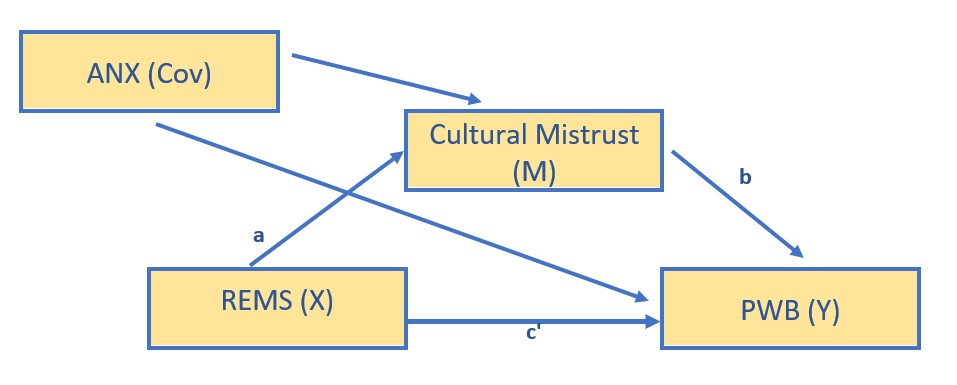
\includegraphics{images/SimpleMed/Kim_wCovs.jpg}
\caption{Image of the simple mediation model from Kim et al.}
\end{figure}

\begin{Shaded}
\begin{Highlighting}[]
\FunctionTok{set.seed}\NormalTok{(}\DecValTok{210410}\NormalTok{)}
\NormalTok{Kim\_fit\_covs }\OtherTok{\textless{}{-}} \StringTok{\textquotesingle{}}
\StringTok{          PWB \textasciitilde{} b*CMI + c\_p*REMS }
\StringTok{          CMI \textasciitilde{}a*REMS}
\StringTok{          CMI \textasciitilde{} covM*ANX}
\StringTok{          PWB \textasciitilde{} covY*ANX}

\StringTok{          indirect :=  a*b}
\StringTok{          direct  := c\_p}
\StringTok{          total\_c  := c\_p + (a*b)}
\StringTok{          \textquotesingle{}}
\NormalTok{Kim\_fit\_covs }\OtherTok{\textless{}{-}} \FunctionTok{sem}\NormalTok{(Kim\_fit\_covs, }\AttributeTok{data =}\NormalTok{ Kim\_df, }\AttributeTok{se=}\StringTok{"bootstrap"}\NormalTok{, }\AttributeTok{missing =} \StringTok{\textquotesingle{}fiml\textquotesingle{}}\NormalTok{)}
\NormalTok{Kcov\_sum }\OtherTok{\textless{}{-}} \FunctionTok{summary}\NormalTok{(Kim\_fit\_covs, }\AttributeTok{standardized=}\NormalTok{T, }\AttributeTok{rsq=}\NormalTok{T, }\AttributeTok{fit=}\ConstantTok{TRUE}\NormalTok{, }\AttributeTok{ci=}\ConstantTok{TRUE}\NormalTok{)}
\NormalTok{Kcov\_ParEsts}\OtherTok{\textless{}{-}} \FunctionTok{parameterEstimates}\NormalTok{(Kim\_fit\_covs, }\AttributeTok{boot.ci.type =} \StringTok{"bca.simple"}\NormalTok{, }\AttributeTok{standardized=}\ConstantTok{TRUE}\NormalTok{)}
\NormalTok{Kcov\_sum}
\end{Highlighting}
\end{Shaded}

\begin{verbatim}
## lavaan 0.6.16 ended normally after 1 iteration
## 
##   Estimator                                         ML
##   Optimization method                           NLMINB
##   Number of model parameters                         9
## 
##   Number of observations                           156
##   Number of missing patterns                         1
## 
## Model Test User Model:
##                                                       
##   Test statistic                                 0.000
##   Degrees of freedom                                 0
## 
## Model Test Baseline Model:
## 
##   Test statistic                               134.067
##   Degrees of freedom                                 5
##   P-value                                        0.000
## 
## User Model versus Baseline Model:
## 
##   Comparative Fit Index (CFI)                    1.000
##   Tucker-Lewis Index (TLI)                       1.000
##                                                       
##   Robust Comparative Fit Index (CFI)             1.000
##   Robust Tucker-Lewis Index (TLI)                1.000
## 
## Loglikelihood and Information Criteria:
## 
##   Loglikelihood user model (H0)               -329.168
##   Loglikelihood unrestricted model (H1)       -329.168
##                                                       
##   Akaike (AIC)                                 676.337
##   Bayesian (BIC)                               703.785
##   Sample-size adjusted Bayesian (SABIC)        675.297
## 
## Root Mean Square Error of Approximation:
## 
##   RMSEA                                          0.000
##   90 Percent confidence interval - lower         0.000
##   90 Percent confidence interval - upper         0.000
##   P-value H_0: RMSEA <= 0.050                       NA
##   P-value H_0: RMSEA >= 0.080                       NA
##                                                       
##   Robust RMSEA                                   0.000
##   90 Percent confidence interval - lower         0.000
##   90 Percent confidence interval - upper         0.000
##   P-value H_0: Robust RMSEA <= 0.050                NA
##   P-value H_0: Robust RMSEA >= 0.080                NA
## 
## Standardized Root Mean Square Residual:
## 
##   SRMR                                           0.000
## 
## Parameter Estimates:
## 
##   Standard errors                            Bootstrap
##   Number of requested bootstrap draws             1000
##   Number of successful bootstrap draws            1000
## 
## Regressions:
##                    Estimate  Std.Err  z-value  P(>|z|) ci.lower ci.upper
##   PWB ~                                                                 
##     CMI        (b)   -0.250    0.092   -2.702    0.007   -0.445   -0.078
##     REMS     (c_p)    0.131    0.479    0.273    0.785   -0.830    1.103
##   CMI ~                                                                 
##     REMS       (a)    3.109    0.318    9.762    0.000    2.483    3.732
##     ANX     (covM)   -0.030    0.058   -0.515    0.607   -0.144    0.083
##   PWB ~                                                                 
##     ANX     (covY)   -0.480    0.064   -7.502    0.000   -0.606   -0.355
##    Std.lv  Std.all
##                   
##    -0.250   -0.230
##     0.131    0.023
##                   
##     3.109    0.599
##    -0.030   -0.036
##                   
##    -0.480   -0.528
## 
## Intercepts:
##                    Estimate  Std.Err  z-value  P(>|z|) ci.lower ci.upper
##    .PWB               5.636    0.277   20.365    0.000    5.091    6.157
##    .CMI               2.032    0.185   10.992    0.000    1.647    2.376
##    Std.lv  Std.all
##     5.636    6.283
##     2.032    2.457
## 
## Variances:
##                    Estimate  Std.Err  z-value  P(>|z|) ci.lower ci.upper
##    .PWB               0.524    0.058    9.086    0.000    0.404    0.631
##    .CMI               0.445    0.050    8.926    0.000    0.345    0.548
##    Std.lv  Std.all
##     0.524    0.651
##     0.445    0.651
## 
## R-Square:
##                    Estimate
##     PWB               0.349
##     CMI               0.349
## 
## Defined Parameters:
##                    Estimate  Std.Err  z-value  P(>|z|) ci.lower ci.upper
##     indirect         -0.776    0.290   -2.680    0.007   -1.376   -0.223
##     direct            0.131    0.479    0.273    0.785   -0.830    1.103
##     total_c          -0.646    0.404   -1.600    0.110   -1.436    0.099
##    Std.lv  Std.all
##    -0.776   -0.138
##     0.131    0.023
##    -0.646   -0.115
\end{verbatim}

\begin{Shaded}
\begin{Highlighting}[]
\NormalTok{Kcov\_ParEsts}
\end{Highlighting}
\end{Shaded}

\begin{verbatim}
##         lhs op       rhs    label    est    se      z pvalue ci.lower ci.upper
## 1       PWB  ~       CMI        b -0.250 0.092 -2.702  0.007   -0.456   -0.085
## 2       PWB  ~      REMS      c_p  0.131 0.479  0.273  0.785   -0.863    1.070
## 3       CMI  ~      REMS        a  3.109 0.318  9.762  0.000    2.433    3.718
## 4       CMI  ~       ANX     covM -0.030 0.058 -0.515  0.607   -0.143    0.083
## 5       PWB  ~       ANX     covY -0.480 0.064 -7.502  0.000   -0.601   -0.353
## 6       PWB ~~       PWB           0.524 0.058  9.086  0.000    0.438    0.669
## 7       CMI ~~       CMI           0.445 0.050  8.926  0.000    0.365    0.568
## 8      REMS ~~      REMS           0.025 0.000     NA     NA    0.025    0.025
## 9      REMS ~~       ANX           0.041 0.000     NA     NA    0.041    0.041
## 10      ANX ~~       ANX           0.974 0.000     NA     NA    0.974    0.974
## 11      PWB ~1                     5.636 0.277 20.365  0.000    5.083    6.152
## 12      CMI ~1                     2.032 0.185 10.992  0.000    1.620    2.357
## 13     REMS ~1                     0.340 0.000     NA     NA    0.340    0.340
## 14      ANX ~1                     2.980 0.000     NA     NA    2.980    2.980
## 15 indirect :=       a*b indirect -0.776 0.290 -2.680  0.007   -1.380   -0.226
## 16   direct :=       c_p   direct  0.131 0.479  0.273  0.785   -0.863    1.070
## 17  total_c := c_p+(a*b)  total_c -0.646 0.404 -1.600  0.110   -1.512    0.035
##    std.lv std.all std.nox
## 1  -0.250  -0.230  -0.230
## 2   0.131   0.023   0.146
## 3   3.109   0.599   3.758
## 4  -0.030  -0.036  -0.036
## 5  -0.480  -0.528  -0.535
## 6   0.524   0.651   0.651
## 7   0.445   0.651   0.651
## 8   0.025   1.000   0.025
## 9   0.041   0.260   0.041
## 10  0.974   1.000   0.974
## 11  5.636   6.283   6.283
## 12  2.032   2.457   2.457
## 13  0.340   2.132   0.340
## 14  2.980   3.020   2.980
## 15 -0.776  -0.138  -0.866
## 16  0.131   0.023   0.146
## 17 -0.646  -0.115  -0.720
\end{verbatim}

\hypertarget{a-figure-and-a-table-1}{%
\subsection{A Figure and a Table}\label{a-figure-and-a-table-1}}

Let's look at a figure to see see if we did what we think we did. And to also get a graphic representation of our results. The semplot package does this easily, but the figure is more statistical than conceptual and would require more tinkering for a journal article.

\begin{Shaded}
\begin{Highlighting}[]
\FunctionTok{semPaths}\NormalTok{(Kim\_fit\_covs, }\CommentTok{\#must identiy the model you want to map}
         \AttributeTok{what =} \StringTok{"est"}\NormalTok{, }\CommentTok{\#"est" plots the estimates, but keeps it greyscale with no fading}
         \CommentTok{\#whatLabels = "stand", \#"stand" changes to standardized values}
         \AttributeTok{layout =} \StringTok{\textquotesingle{}tree\textquotesingle{}}\NormalTok{, }\AttributeTok{rotation =} \DecValTok{2}\NormalTok{, }\CommentTok{\#together, puts predictors on left, IVs on right }
         \AttributeTok{edge.label.cex =} \FloatTok{1.00}\NormalTok{, }\CommentTok{\#font size of parameter values}
         \CommentTok{\#edge.color = "black", \#overwrites the green/black coloring}
         \AttributeTok{sizeMan=}\DecValTok{10}\NormalTok{, }\CommentTok{\#size of squares/observed/"manifest" variables}
         \AttributeTok{fade=}\ConstantTok{FALSE}\NormalTok{, }\CommentTok{\#if TRUE, there lines are faded such that weaker lines correspond with lower values {-}{-} a cool effect, but tough for journals}
         \AttributeTok{esize=}\DecValTok{2}\NormalTok{, }
         \AttributeTok{asize=}\DecValTok{3}\NormalTok{,}
         \CommentTok{\#label.prop = .5,}
         \AttributeTok{label.font =} \FloatTok{2.5}\NormalTok{, }\CommentTok{\#controls size (I think) of font for labels}
         \AttributeTok{label.scale =} \ConstantTok{TRUE}\NormalTok{, }\CommentTok{\#if false, the labels will not scale to fit inside the nodes}
         \AttributeTok{nDigits =} \DecValTok{3}\NormalTok{, }\CommentTok{\#decimal places (default is 2)}
         \AttributeTok{residuals =} \ConstantTok{FALSE}\NormalTok{,}\CommentTok{\#excludes residuals (and variances) from the path diagram}
         \AttributeTok{nCharNodes =} \DecValTok{0}\NormalTok{, }\CommentTok{\#specifies how many characters to abbreviate variable lables; default is 3.  If 0, uses your entire variable label and adjusts fontsize (which could be a downside)}
         \AttributeTok{intercepts =} \ConstantTok{FALSE}\NormalTok{, }\CommentTok{\#gets rid of those annoying triangles (intercepts) in the path diagram)}
\NormalTok{)}
\FunctionTok{title}\NormalTok{(}\StringTok{"Entrepreneurial Withdrawal by eDistress via Negative Affect (\& some covariates("}\NormalTok{)}
\end{Highlighting}
\end{Shaded}

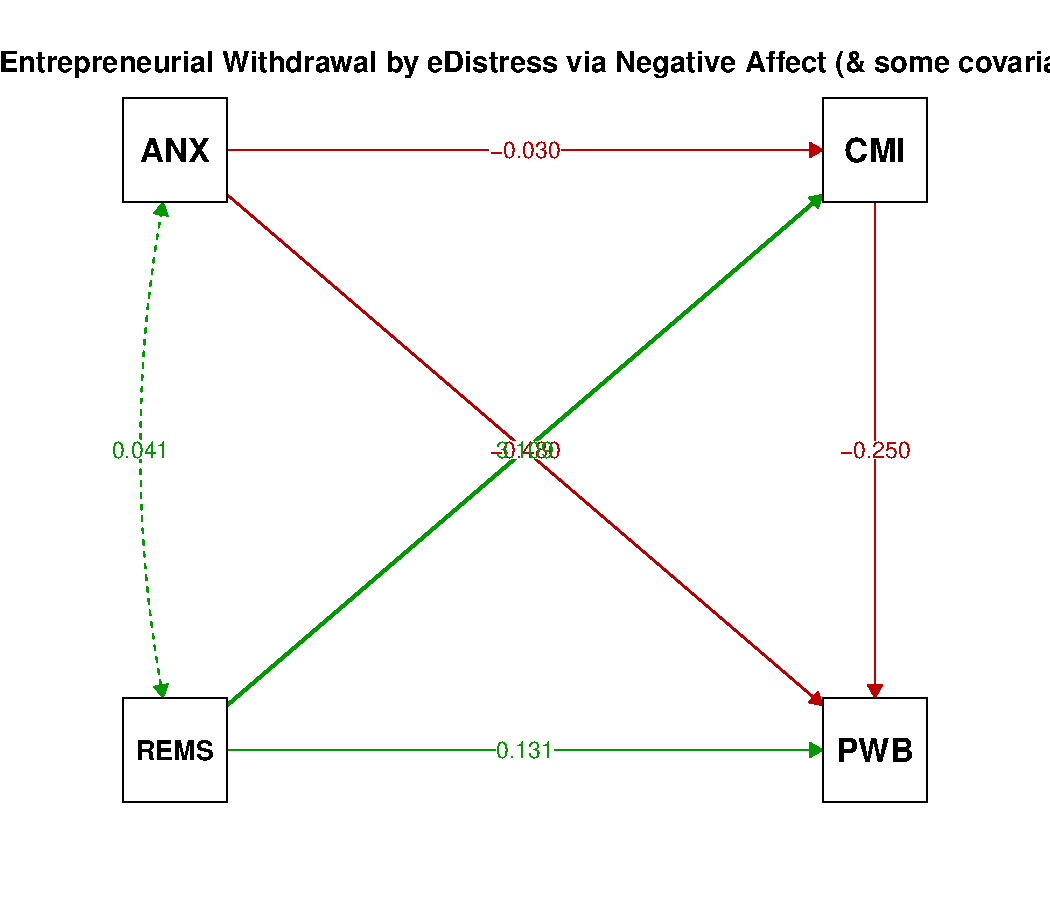
\includegraphics{05-SimpleMed_files/figure-latex/semPLOT for model w covs-1.pdf}

The path coefficients appear to be correct, but this is really a statistical map and doesn't relay the concept of mediation well.

Below is code to create an outfile that could help with creating a table in a word document or spreadsheet. There will be output that is produced with SEM models that won't be relevant for this project.

\begin{Shaded}
\begin{Highlighting}[]
\NormalTok{KimCOVTab }\OtherTok{\textless{}{-}} \FunctionTok{semTable}\NormalTok{(Kim\_fit\_covs, }\AttributeTok{columns =} \FunctionTok{c}\NormalTok{(}\StringTok{"est"}\NormalTok{, }\StringTok{"se"}\NormalTok{, }\StringTok{"p"}\NormalTok{, }\StringTok{"rsquare"}\NormalTok{),  }\AttributeTok{columnLabels =} \FunctionTok{c}\NormalTok{(}\AttributeTok{eststars =} \StringTok{"Estimate"}\NormalTok{), }\AttributeTok{paramSets =} \FunctionTok{c}\NormalTok{(}\StringTok{"composites"}\NormalTok{, }\StringTok{"loadings"}\NormalTok{, }\StringTok{"slopes"}\NormalTok{, }\StringTok{"intercepts"}\NormalTok{, }\StringTok{"residualvariances"}\NormalTok{), }\AttributeTok{file =} \StringTok{"ESTRESScov\_fitTABLE"}\NormalTok{, }\AttributeTok{type =} \StringTok{"csv"}\NormalTok{, }\AttributeTok{print.results =} \ConstantTok{TRUE}\NormalTok{)}
\end{Highlighting}
\end{Shaded}

Table 2

\begin{longtable}[]{@{}
  >{\raggedright\arraybackslash}p{(\columnwidth - 0\tabcolsep) * \real{1.0000}}@{}}
\toprule\noalign{}
\begin{minipage}[b]{\linewidth}\raggedright
Model Coefficients Assessing Cultural Mistrust as a Mediator Between Racial Microaggressions and Well-Being
\end{minipage} \\
\midrule\noalign{}
\endhead
\bottomrule\noalign{}
\endlastfoot
\end{longtable}

\begin{longtable}[]{@{}
  >{\raggedright\arraybackslash}p{(\columnwidth - 6\tabcolsep) * \real{0.1969}}
  >{\centering\arraybackslash}p{(\columnwidth - 6\tabcolsep) * \real{0.3228}}
  >{\centering\arraybackslash}p{(\columnwidth - 6\tabcolsep) * \real{0.0551}}
  >{\centering\arraybackslash}p{(\columnwidth - 6\tabcolsep) * \real{0.4252}}@{}}
\toprule\noalign{}
\endhead
\bottomrule\noalign{}
\endlastfoot
& Cultural Mistrust (M) & & Well-Being (Y) \\
\end{longtable}

\begin{longtable}[]{@{}
  >{\raggedright\arraybackslash}p{(\columnwidth - 16\tabcolsep) * \real{0.1393}}
  >{\centering\arraybackslash}p{(\columnwidth - 16\tabcolsep) * \real{0.0574}}
  >{\centering\arraybackslash}p{(\columnwidth - 16\tabcolsep) * \real{0.1148}}
  >{\centering\arraybackslash}p{(\columnwidth - 16\tabcolsep) * \real{0.1311}}
  >{\centering\arraybackslash}p{(\columnwidth - 16\tabcolsep) * \real{0.1393}}
  >{\centering\arraybackslash}p{(\columnwidth - 16\tabcolsep) * \real{0.0574}}
  >{\centering\arraybackslash}p{(\columnwidth - 16\tabcolsep) * \real{0.1066}}
  >{\centering\arraybackslash}p{(\columnwidth - 16\tabcolsep) * \real{0.1311}}
  >{\centering\arraybackslash}p{(\columnwidth - 16\tabcolsep) * \real{0.1230}}@{}}
\toprule\noalign{}
\endhead
\bottomrule\noalign{}
\endlastfoot
Antecedent & path & \(B\) & \(SE\) & \(p\) & path & \(B\) & \(SE\) & \(p\) \\
constant & \(i_{M}\) & 2.032 & 0.185 & 0.000 & \(i_{Y}\) & 5.636 & 0.277 & 0.000 \\
REMS (X) & \(a\) & 3.109 & 0.318 & 0.000 & \(c'\) & 0.131 & 0.479 & 0.785 \\
CMI (M) & & & & & \(b\) & -0.250 & 0.092 & 0.007 \\
ANX (Cov) & & -0.030 & 0.058 & 0.607 & & -0.480 & 0.064 & 0.000 \\
\end{longtable}

\begin{longtable}[]{@{}
  >{\raggedright\arraybackslash}p{(\columnwidth - 6\tabcolsep) * \real{0.1969}}
  >{\centering\arraybackslash}p{(\columnwidth - 6\tabcolsep) * \real{0.3858}}
  >{\centering\arraybackslash}p{(\columnwidth - 6\tabcolsep) * \real{0.0551}}
  >{\centering\arraybackslash}p{(\columnwidth - 6\tabcolsep) * \real{0.3622}}@{}}
\toprule\noalign{}
\endhead
\bottomrule\noalign{}
\endlastfoot
& \(R^2\) = & & \(R^2\) = \\
\end{longtable}

\hypertarget{apa-style-write-up}{%
\subsection{APA Style Write-up}\label{apa-style-write-up}}

There are varying models for reporting the results of mediation. The Kim et al. \citep{kim_racial_2017} writeup is a great example. Rather than copying it directly, I have modeled my table after the ones in Hayes \citeyearpar{hayes_introduction_2018} text. You'll notice that information in the table and text are minimally overlapping. APA style cautions us against redundancy in text and table.

\textbf{Results}

A simple mediation model examined the degree to which cultural mistrust mediated the effect of racial microaggressions on psychological well-being. Using the \emph{lavaan} package (v 0.6-7) in R, coefficients for the each path, the indirect effect, and total effects were calculated. The effect of covariate, anxiety, was mapped onto both the mediator and dependent variable. These values are presented in Table 3 and illustrated in Figure 3. Results suggested that of the variance in cultural mistrust and of the variance in well-being were accounted for by the model. Supporting the notion of a mediated model, there was a statistically significant indirect effect (\(B\) = -0.776, \(p\) = 0.007, CI95 -1.380 to -0.226) in combination with a non-significant direct effect (\(B\) = 0.131, \(p\) = 0.785, CI95 -0.863 to 1.070). Curiously, though, the total effect (\(B\) = -0.646, \(p\) = 0.110, CI95 -1.512 to 0.035) was also non-significant.

\hypertarget{residual-and-related-questions}{%
\section{Residual and Related Questions\ldots{}}\label{residual-and-related-questions}}

..that you might have; or at least I had, but if had answered them earlier it would have disrupt the flow.

\begin{enumerate}
\def\labelenumi{\arabic{enumi}.}
\tightlist
\item
  Are you sure you can claim a significant indirect effect in the presence of a non-significant total effect? Hayes \citeyearpar{hayes_introduction_2018} is.

  \begin{itemize}
  \tightlist
  \item
    In the section subtitled, ``What about Baron \& Kenny'' (chapter 4), Hayes argues from both logical/philosophical and statistical perspectives that the size of the total effect does not constrain or determine the size of the indirect effect. That is, an indirect effect can be different from zero even when the total effect is not (pp.~117-119).\\
  \end{itemize}
\item
  The output we get is different from the output in the journal article being used as the research vignette. Why? And should we worry about it?

  \begin{itemize}
  \tightlist
  \item
    We are simulating data. This gives us some advantages in that (unless we specify it), we never have missingness and our variables should be normally distributed. Because we are working from means, standard deviations, and correlations, our data will never be the same as the original researcher. That said, we can compare our results to the journal to \emph{check out work.} In fact, in this very chapter, I got turned around (e.g., first accidentally swapping the mediator and IV; then using the wrong DV) and was able to compare my work against the journal article to correct my errors.
  \end{itemize}
\item
  Some of the statistics you are reporting are different than the ones in Hayes and the ones that use the PROCESS macro (e.g., what happened to the \emph{F} test)?

  \begin{itemize}
  \tightlist
  \item
    The default estimator for \emph{lavaan} is maximum likelihood (ML) and Hayes uses ordinary least squares (OLS). This affects both the values of coefficients, standard errors, AND the type of statistics that are reported.
  \item
    You can ask for OLS regression by adding the statement ``estimator =''GLS''. Even with this option, I have not discovered a way to obtain the \emph{F} tests for the overall model. Researchers seem to be comfortable with this, even asking for less than we did (e.g., many do not request R square).
  \item
    Best I can tell, researchers who do want this might use a combination of packages, using GLS estimators in \emph{lavaan} (this easily gets them the bootstrapped CIs) and the move to a different regression package to get the intercepts and \emph{F} tests. If I did this I would triple check to make sure that all the output really lined up.
  \end{itemize}
\item
  Why did we ignore the traditional fit statistics associated with structural equation modeling (e.g., CFI, RMSEA).

  \begin{itemize}
  \tightlist
  \item
    I hesitate to do this with models that do not include latent variables. Therefore, we asked for an ``in-between'' amount of info that should be sufficient for publication submission (any editor may have their own preferences and ask for more).
  \end{itemize}
\item
  What if I have missing data?

  \begin{itemize}
  \tightlist
  \item
    When we enter the \emph{lavaan} world we do get options other than multiple imputation. In today's example we used the ``sem'' fitting function. Unless otherwise specified, listwise deletion (deleting the entire case when one of its variables is used to estimate the model) is the default in \emph{lavaan}. If data are MCAR or MAR, you can add the argument \emph{missing = ``ml''} (or its alias \emph{missing = ``fiml''}). More here \url{https://users.ugent.be/~yrosseel/lavaan/lavaan2.pdf} on the 1.7/Missing data in lavaan slide.
  \item
    That said, the type of estimator matters. If you estimate your data with GLS (generalized least squares) or WLS (weighted least squares), you are required to have complete data (however you got it). We used maximum likelihood and, even though we had non-missing data, I used the \emph{missing = ``fiml''} code.
  \end{itemize}
\end{enumerate}

\hypertarget{practice-problems-4}{%
\section{Practice Problems}\label{practice-problems-4}}

The three problems described below are designed to grow with the subsequent chapters on complex mediation and conditional process analysis (i.e,. moderated mediation). Therefore, I recommend that you select a dataset that includes at least four variables. If you are new to this topic, you may wish to select variables that are all continuously scaled. The IV and moderator (subsequent chapters) could be categorical (if they are dichotomous, please use 0/1 coding; if they have more than one category it is best if they are ordered). You will likely encounter challenges that were not covered in this chapter. Search for and try out solutions, knowing that there are multiple paths through the analysis.

The suggested practice problem for this chapter is to conduct a simple mediation.

\hypertarget{problem-1-rework-the-research-vignette-as-demonstrated-but-change-the-random-seed}{%
\subsection{Problem \#1: Rework the research vignette as demonstrated, but change the random seed}\label{problem-1-rework-the-research-vignette-as-demonstrated-but-change-the-random-seed}}

If this topic feels a bit overwhelming, simply change the random seed in the data simulation, then rework the problem. This should provide minor changes to the data (maybe in the second or third decimal point), but the results will likely be very similar.

\begin{longtable}[]{@{}
  >{\raggedright\arraybackslash}p{(\columnwidth - 4\tabcolsep) * \real{0.7642}}
  >{\centering\arraybackslash}p{(\columnwidth - 4\tabcolsep) * \real{0.1220}}
  >{\centering\arraybackslash}p{(\columnwidth - 4\tabcolsep) * \real{0.1138}}@{}}
\toprule\noalign{}
\begin{minipage}[b]{\linewidth}\raggedright
Assignment Component
\end{minipage} & \begin{minipage}[b]{\linewidth}\centering
\end{minipage} & \begin{minipage}[b]{\linewidth}\centering
\end{minipage} \\
\midrule\noalign{}
\endhead
\bottomrule\noalign{}
\endlastfoot
1. Assign each variable to the X, Y, or M roles (ok but not required to include a cov) & 5 & \_\_\_\_\_ \\
2. Specify and run the lavaan model & 5 & \_\_\_\_\_ \\
3. Use semPlot to create a figure & 5 & \_\_\_\_\_ \\
4. Create a table that includes regression output for the M and Y variables & 5 & \_\_\_\_\_ \\
5. Represent your work in an APA-style write-up & 5 & \_\_\_\_\_ \\
6. Explanation to grader & 5 & \_\_\_\_\_ \\
7. Be able to hand-calculate the indirect, direct, and total effects from the a, b, \& c' paths & 5 & \_\_\_\_\_ \\
\textbf{Totals} & 35 & \_\_\_\_\_ \\
\end{longtable}

\hypertarget{problem-2-rework-the-research-vignette-but-swap-one-or-more-variables}{%
\subsection{Problem \#2: Rework the research vignette, but swap one or more variables}\label{problem-2-rework-the-research-vignette-but-swap-one-or-more-variables}}

Use the simulated data, but select one of the other models that was evaluated in the Kim et al. \citeyearpar{kim_racial_2017} study. Compare your results to those reported in the mansucript.

\begin{longtable}[]{@{}
  >{\raggedright\arraybackslash}p{(\columnwidth - 4\tabcolsep) * \real{0.7642}}
  >{\centering\arraybackslash}p{(\columnwidth - 4\tabcolsep) * \real{0.1220}}
  >{\centering\arraybackslash}p{(\columnwidth - 4\tabcolsep) * \real{0.1138}}@{}}
\toprule\noalign{}
\begin{minipage}[b]{\linewidth}\raggedright
Assignment Component
\end{minipage} & \begin{minipage}[b]{\linewidth}\centering
\end{minipage} & \begin{minipage}[b]{\linewidth}\centering
\end{minipage} \\
\midrule\noalign{}
\endhead
\bottomrule\noalign{}
\endlastfoot
1. Assign each variable to the X, Y, or M roles (ok but not required to include a cov) & 5 & \_\_\_\_\_ \\
2. Specify and run the lavaan model & 5 & \_\_\_\_\_ \\
3. Use semPlot to create a figure & 5 & \_\_\_\_\_ \\
4. Create a table that includes regression output for the M and Y variables & 5 & \_\_\_\_\_ \\
5. Represent your work in an APA-style write-up & 5 & \_\_\_\_\_ \\
6. Explanation to grader & 5 & \_\_\_\_\_ \\
7. Be able to hand-calculate the indirect, direct, and total effects from the a, b, \& c' paths & 5 & \_\_\_\_\_ \\
\textbf{Totals} & 35 & \_\_\_\_\_ \\
\end{longtable}

\hypertarget{problem-3-use-other-data-that-is-available-to-you}{%
\subsection{Problem \#3: Use other data that is available to you}\label{problem-3-use-other-data-that-is-available-to-you}}

Using data for which you have permission and access (e.g., IRB approved data you have collected or from your lab; data you simulate from a published article; data from an open science repository; data from other chapters in this OER), complete a simple mediation.

\begin{longtable}[]{@{}
  >{\raggedright\arraybackslash}p{(\columnwidth - 4\tabcolsep) * \real{0.7642}}
  >{\centering\arraybackslash}p{(\columnwidth - 4\tabcolsep) * \real{0.1220}}
  >{\centering\arraybackslash}p{(\columnwidth - 4\tabcolsep) * \real{0.1138}}@{}}
\toprule\noalign{}
\begin{minipage}[b]{\linewidth}\raggedright
Assignment Component
\end{minipage} & \begin{minipage}[b]{\linewidth}\centering
\end{minipage} & \begin{minipage}[b]{\linewidth}\centering
\end{minipage} \\
\midrule\noalign{}
\endhead
\bottomrule\noalign{}
\endlastfoot
1. Assign each variable to the X, Y, or M roles (ok but not required to include a cov) & 5 & \_\_\_\_\_ \\
2. Specify and run the lavaan model & 5 & \_\_\_\_\_ \\
3. Use semPlot to create a figure & 5 & \_\_\_\_\_ \\
4. Create a table that includes regression output for the M and Y variables & 5 & \_\_\_\_\_ \\
5. Represent your work in an APA-style write-up & 5 & \_\_\_\_\_ \\
6. Explanation to grader & 5 & \_\_\_\_\_ \\
7. Be able to hand-calculate the indirect, direct, and total effects from the a, b, \& c' paths & 5 & \_\_\_\_\_ \\
\textbf{Totals} & 35 & \_\_\_\_\_ \\
\end{longtable}

\hypertarget{CompMed}{%
\chapter{Complex Mediation}\label{CompMed}}

\href{https://spu.hosted.panopto.com/Panopto/Pages/Viewer.aspx?pid=6991fd3d-22b6-44f5-ab5b-ad1000314b7f}{Screencasted Lecture Link}

The focus of this chapter is the extension of simple mediation to models with multiple mediatrs. In these models with greater complexity we look at both parallel and serial mediation. There is also more elaboration on some of the conceptual issues related to the estimation of indirect effects.

\hypertarget{navigating-this-lesson-5}{%
\section{Navigating this Lesson}\label{navigating-this-lesson-5}}

There is about 1 hour and 20 minutes of lecture. If you work through the materials with me it would be plan for an additional two hours.

While the majority of R objects and data you will need are created within the R script that sources the chapter, there are a few that cannot be created from within the R framework. Additionally, sometimes links fail. All original materials are provided at the \href{https://https://github.com/lhbikos/ReC_MultivModel}{Github site} that hosts the book. More detailed guidelines for ways to access all these materials are provided in the OER's \protect\hyperlink{ReCintro}{introduction}

\hypertarget{learning-objectives-5}{%
\subsection{Learning Objectives}\label{learning-objectives-5}}

Learning objectives from this lecture include the following:

\begin{itemize}
\tightlist
\item
  Define \emph{epiphenomality} and explain how it is related to (and supports the notion of) multiple mediation.
\item
  Distinguish between parallel and serial mediation models.
\item
  Locate and interpret \emph{lavaan} output from multiply mediated models including
\item
  identifying coefficients,
\item
  percentage of variance accounted for,\\
\item
  all the effects (total, direct, indirec. total indirect),
\item
  contrasts.
\item
  Explain the limitations of the classic approach \citep{baron_moderator-mediator_1986} to mediation.
\end{itemize}

\hypertarget{planning-for-practice-5}{%
\subsection{Planning for Practice}\label{planning-for-practice-5}}

The suggestions for practice in this chapter include conducting parallel, serial, and/or mediation models. Options of graded complexity could incude:

\begin{itemize}
\tightlist
\item
  Rework the problem in the chapter by changing the random seed in the code that simulates the data. This should provide minor changes to the data, but the results will likely be very similar.
\item
  There are a number of variables in the dataset that sourced the research vignettes for this and the prior chapter on \protect\hyperlink{SimpleMed}{simple mediation}. Swap out one or more variables in a parallel or serial (or both) model.
\item
  Conduct a parallel or serial (or both) mediation with data to which you have access. This could include data you simulate on your own or from a published article.
\end{itemize}

\hypertarget{readings-resources-5}{%
\subsection{Readings \& Resources}\label{readings-resources-5}}

In preparing this chapter, I drew heavily from the following resource(s). Other resources are cited (when possible, linked) in the text with complete citations in the reference list.

\begin{itemize}
\tightlist
\item
  Hayes, A. F. (2018). \emph{Introduction to mediation, moderation, and conditional process anlaysis: A regression-based approach}. New York, NY: Guilford Press. Available as an ebook from the SPU library: \url{https://ebookcentral-proquest-com.ezproxy.spu.edu/lib/spu/detail.action?docID=5109647}

  \begin{itemize}
  \tightlist
  \item
    \textbf{Chapter 5: More than One Mediator}: This chapter walks the reader through parallel and serial mediation models. We will do both!
  \item
    \textbf{Appendix A: Using Process}: An essential tool for PROCESS users because, even when we are in the R environment, this is the ``idea book.'' That is, the place where all the path models are presented in figures.
  \end{itemize}
\item
  Lewis, J. A., Williams, M. G., Peppers, E. J., \& Gadson, C. A. (2017). Applying intersectionality to explore the relations between gendered racism and health among Black women. \emph{Journal of Counseling Psychology}, \emph{64}(5), 475--486. \url{https://doi-org.ezproxy.spu.edu/10.1037/cou0000231}
\end{itemize}

\hypertarget{packages-5}{%
\subsection{Packages}\label{packages-5}}

The script below will (a) check to see if the following packages are installed on your computer and, if not (b) install them.

\begin{Shaded}
\begin{Highlighting}[]
\CommentTok{\#will install the package if not already installed}
\ControlFlowTok{if}\NormalTok{(}\SpecialCharTok{!}\FunctionTok{require}\NormalTok{(lavaan))\{}\FunctionTok{install.packages}\NormalTok{(}\StringTok{"lavaan"}\NormalTok{)\}}
\ControlFlowTok{if}\NormalTok{(}\SpecialCharTok{!}\FunctionTok{require}\NormalTok{(semPlot))\{}\FunctionTok{install.packages}\NormalTok{(}\StringTok{"semPlot"}\NormalTok{)\}}
\ControlFlowTok{if}\NormalTok{(}\SpecialCharTok{!}\FunctionTok{require}\NormalTok{(tidyverse))\{}\FunctionTok{install.packages}\NormalTok{(}\StringTok{"tidyverse"}\NormalTok{)\}}
\ControlFlowTok{if}\NormalTok{(}\SpecialCharTok{!}\FunctionTok{require}\NormalTok{(psych))\{}\FunctionTok{install.packages}\NormalTok{(}\StringTok{"psych"}\NormalTok{)\}}
\ControlFlowTok{if}\NormalTok{(}\SpecialCharTok{!}\FunctionTok{require}\NormalTok{(apaTables))\{}\FunctionTok{install.packages}\NormalTok{(}\StringTok{"apaTables"}\NormalTok{)\}}
\ControlFlowTok{if}\NormalTok{(}\SpecialCharTok{!}\FunctionTok{require}\NormalTok{(formattable))\{}\FunctionTok{install.packages}\NormalTok{(}\StringTok{"formattable"}\NormalTok{)\}}
\end{Highlighting}
\end{Shaded}

\hypertarget{complex-mediation}{%
\section{Complex Mediation}\label{complex-mediation}}

The simple mediation model is quite popular, but also limiting in that it:

\begin{itemize}
\tightlist
\item
  frequently oversimplifies the processes we want to study, and
\item
  is likely mis-specified, in that there are unmodeled mechanisms.
\end{itemize}

Hayes \citeyearpar{hayes_introduction_2018} identified four reasons to consider multiply mediated models:

\begin{itemize}
\tightlist
\item
  We are generally interested in MULTIPLE mechanisms
\item
  A mechanism (such as a mediator) in the model, might, itself be mediated (i.e., mediated mediation)
\item
  \emph{Epiphenomenality} (``unknown confounds''): a proposed mediator could be related to an outcome not because it causes the outcome, but because it is correlated with another variable that is causally influencing the outcome. This is a noncausal alternative explanation for an association.
\item
  Including multiple mediators allows formal comparison of the strength of the mediating mechanisms.
\end{itemize}

There are two multiple mediator models that we will consider: parallel, serial.

\hypertarget{parallel-mediation}{%
\section{Parallel Mediation}\label{parallel-mediation}}

\textbf{Parallel multiple mediation}: An antecedent variable X is modeled as influencing consequent Y directly as well as indirectly through two or more mediators, with the condition that no mediator causally influences another \citep[p.~149]{hayes_introduction_2018}

With multiple mediation we introduce additional effects:

\begin{itemize}
\tightlist
\item
  \emph{Direct effect}, \(c'\) (this is not new) quantifies how much two cases that differ by a unit on X are estimated to differ on Y -- independent of all mediators.
\item
  \emph{Specific indirect effect}, \(a_{i}b_{i}\), the individual mediated effects
\item
  \emph{Total indirect effects }, \(\sum_{i=1}^{k}a_{i}b_{i}\) the sum of the values of the specific indirect effects. The total indirect effect can also be calculated by subtracting the direct effects from the total effects: \(c - c'\)
\item
  \emph{Total effect of X on Y}, \(c = c' + \sum_{i=1}^{k}a_{i}b_{i}\) (also not new) the sum of the direct and indirect effects. The total effect can also be estimated by regressing Y on X alone.
\item
  \emph{Contrasts} allow us to directly compare separate mediating effects to see if one indirect effect is stronger than the other.
\end{itemize}

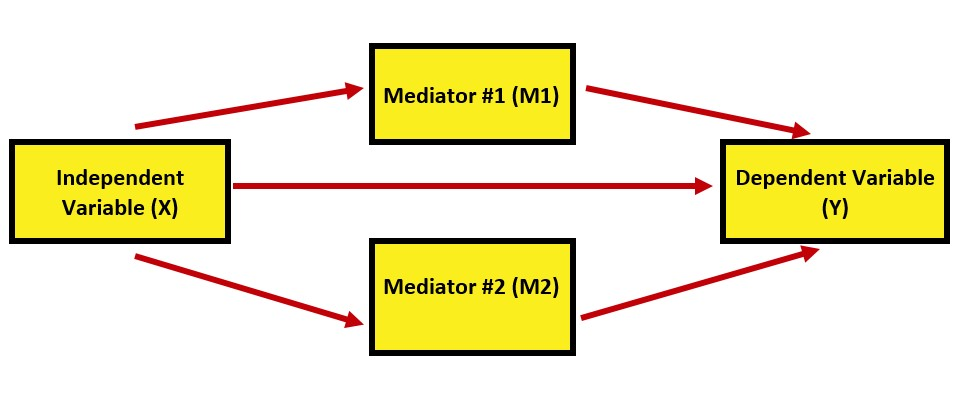
\includegraphics{images/CompMed/ParaMed.jpg} In this parallel model, we can describe these effects this way:

\begin{itemize}
\tightlist
\item
  \emph{Direct effect}: The effect of IV on the DV, accounting for two mediators (indirect effects) in the model.
\item
  \emph{Specific indirect effects}: There are indirect (or mediating) paths from the IV to the DV; through M1 and M2, respectively.
\item
  \emph{Total indirect effect of X on Y}: A sum of the value of indirect effects through the specific indirect effects (M1 and M2).
\item
  \emph{Total effect}: The sum of the direct and indirect effects. Also calculated by regressing Y (dependent variable) on X (independent variable) alone, without any other variables in the model.
\end{itemize}

Recall that for a complex mediation to be parallel, there can be no causal links between mediators. This is true in this example.

As before, let's work a mechanical example with simulated data that assures a statistically significant outcome. Credit to this example is from the PAULOTOFFANIN website \citep{toffanin_multiple-mediator_2017}.

\hypertarget{a-mechanical-example}{%
\subsection{A Mechanical Example}\label{a-mechanical-example}}

We can bake our own data by updating the script we used in simple mediation to add a second mediator.

\hypertarget{data-simulation}{%
\subsubsection{Data Simulation}\label{data-simulation}}

\begin{Shaded}
\begin{Highlighting}[]
\CommentTok{\# Concerned that identical variable names across book chapters may be problematic, I\textquotesingle{}m adding "p" in front the "Data" variable.}
\FunctionTok{set.seed}\NormalTok{(}\DecValTok{210417}\NormalTok{)}
\NormalTok{X }\OtherTok{\textless{}{-}} \FunctionTok{rnorm}\NormalTok{(}\DecValTok{100}\NormalTok{)}
\NormalTok{M1 }\OtherTok{\textless{}{-}} \FloatTok{0.5}\SpecialCharTok{*}\NormalTok{X }\SpecialCharTok{+} \FunctionTok{rnorm}\NormalTok{(}\DecValTok{100}\NormalTok{)}
\NormalTok{M2 }\OtherTok{\textless{}{-}} \SpecialCharTok{{-}}\FloatTok{0.35}\SpecialCharTok{*}\NormalTok{X }\SpecialCharTok{+} \FunctionTok{rnorm}\NormalTok{(}\DecValTok{100}\NormalTok{)}
\NormalTok{Y }\OtherTok{\textless{}{-}} \FloatTok{0.7}\SpecialCharTok{*}\NormalTok{M2 }\SpecialCharTok{+} \FloatTok{0.48}\SpecialCharTok{*}\NormalTok{M1 }\SpecialCharTok{+} \FunctionTok{rnorm}\NormalTok{(}\DecValTok{100}\NormalTok{)}
\NormalTok{pData }\OtherTok{\textless{}{-}} \FunctionTok{data.frame}\NormalTok{(}\AttributeTok{X =}\NormalTok{ X, }\AttributeTok{Y =}\NormalTok{ Y, }\AttributeTok{M1 =}\NormalTok{ M1, }\AttributeTok{M2 =}\NormalTok{ M2)}
\end{Highlighting}
\end{Shaded}

Using what we learned in conducting a simple mediation in \emph{lavaan}, we can look at the figure of our proposed model and \emph{backwardstrace} the paths to write the code.

Remember\ldots{}

\begin{itemize}
\item
  The model exists between 2 single quotation marks (the odd looking ' and ' at the beginning and end).
\item
  You can write the Y as I have done in the R chunk below, or you can write the Y separately from each arrow, such as

  \begin{itemize}
  \tightlist
  \item
    Y \textasciitilde{} b1*M1
  \item
    Y \textasciitilde{} b2*M2
  \item
    Y \textasciitilde{} c\_p*X
  \end{itemize}
\item
  Everything else transfers from our simple mediation, remember that

  \begin{itemize}
  \tightlist
  \item
    the asterisk (``*``) allows us to assign labels (a1, a2, b1, b2, etc.) to the paths; these are helpful for intuitive interpretation
  \item
    that eyes/nose notation (:=) is used when creating a new variable that is a function of variables in the model, but not in the dataset (i.e., the a and b path).
  \item
    in traditional mediation speak, the direct path from X to Y is c' (c prime) and the total effect of X to Y (with nothing else in the model) is just c.~Hence the c\_p label for c prime.
  \end{itemize}
\item
  Something new: the \emph{contrast} statement (only one in this example, but you could have more) allows us to compare the indirect effects to each other. We specify it in the lavaan model, but then need to test it in a subsequent set of script.
\item
  \emph{Note}: In the online example, the writer adds code to correlate M1 and M2. This didn't/doesn't seem right to me and then, later, when we amend it to be a serial model, it made even less sense to have them be correlated.
\end{itemize}

\hypertarget{specifying-lavaan-code}{%
\subsubsection{\texorpdfstring{Specifying \emph{lavaan} code}{Specifying lavaan code}}\label{specifying-lavaan-code}}

\begin{Shaded}
\begin{Highlighting}[]
\FunctionTok{library}\NormalTok{(lavaan)}
\end{Highlighting}
\end{Shaded}

\begin{verbatim}
## This is lavaan 0.6-16
## lavaan is FREE software! Please report any bugs.
\end{verbatim}

\begin{Shaded}
\begin{Highlighting}[]
\FunctionTok{set.seed}\NormalTok{(}\DecValTok{210418}\NormalTok{)}
\NormalTok{parallel\_med }\OtherTok{\textless{}{-}} \StringTok{\textquotesingle{}}
\StringTok{    Y \textasciitilde{} b1*M1 + b2*M2 + c\_p*X}
\StringTok{    M1 \textasciitilde{} a1*X}
\StringTok{    M2 \textasciitilde{} a2*X}
\StringTok{    indirect1 := a1 * b1}
\StringTok{    indirect2 := a2 * b2}
\StringTok{    contrast := indirect1 {-} indirect2}
\StringTok{    total\_indirects := indirect1 + indirect2}
\StringTok{    total\_c    := c\_p + (indirect1) + (indirect2)}
\StringTok{    direct := c\_p}
\StringTok{ \textquotesingle{}}
\NormalTok{parallel\_fit }\OtherTok{\textless{}{-}} \FunctionTok{sem}\NormalTok{(parallel\_med, }\AttributeTok{data =}\NormalTok{ pData, }\AttributeTok{se =} \StringTok{"bootstrap"}\NormalTok{, }\AttributeTok{missing =} \StringTok{\textquotesingle{}fiml\textquotesingle{}}\NormalTok{, }\AttributeTok{bootstrap =} \DecValTok{1000}\NormalTok{)}
\NormalTok{pfit\_sum }\OtherTok{\textless{}{-}} \FunctionTok{summary}\NormalTok{(parallel\_fit, }\AttributeTok{standardized =} \ConstantTok{TRUE}\NormalTok{, }\AttributeTok{rsq=}\NormalTok{T, }\AttributeTok{fit=}\ConstantTok{TRUE}\NormalTok{, }\AttributeTok{ci=}\ConstantTok{TRUE}\NormalTok{)    }
\NormalTok{pfit\_ParEsts }\OtherTok{\textless{}{-}} \FunctionTok{parameterEstimates}\NormalTok{(parallel\_fit, }\AttributeTok{boot.ci.type =} \StringTok{"bca.simple"}\NormalTok{, }\AttributeTok{standardized=}\ConstantTok{TRUE}\NormalTok{)}
\NormalTok{pfit\_sum}
\end{Highlighting}
\end{Shaded}

\begin{verbatim}
## lavaan 0.6.16 ended normally after 3 iterations
## 
##   Estimator                                         ML
##   Optimization method                           NLMINB
##   Number of model parameters                        11
## 
##   Number of observations                           100
##   Number of missing patterns                         1
## 
## Model Test User Model:
##                                                       
##   Test statistic                                 0.095
##   Degrees of freedom                                 1
##   P-value (Chi-square)                           0.757
## 
## Model Test Baseline Model:
## 
##   Test statistic                                91.109
##   Degrees of freedom                                 6
##   P-value                                        0.000
## 
## User Model versus Baseline Model:
## 
##   Comparative Fit Index (CFI)                    1.000
##   Tucker-Lewis Index (TLI)                       1.064
##                                                       
##   Robust Comparative Fit Index (CFI)             1.000
##   Robust Tucker-Lewis Index (TLI)                1.064
## 
## Loglikelihood and Information Criteria:
## 
##   Loglikelihood user model (H0)               -425.933
##   Loglikelihood unrestricted model (H1)       -425.885
##                                                       
##   Akaike (AIC)                                 873.866
##   Bayesian (BIC)                               902.522
##   Sample-size adjusted Bayesian (SABIC)        867.782
## 
## Root Mean Square Error of Approximation:
## 
##   RMSEA                                          0.000
##   90 Percent confidence interval - lower         0.000
##   90 Percent confidence interval - upper         0.181
##   P-value H_0: RMSEA <= 0.050                    0.785
##   P-value H_0: RMSEA >= 0.080                    0.178
##                                                       
##   Robust RMSEA                                   0.000
##   90 Percent confidence interval - lower         0.000
##   90 Percent confidence interval - upper         0.181
##   P-value H_0: Robust RMSEA <= 0.050             0.785
##   P-value H_0: Robust RMSEA >= 0.080             0.178
## 
## Standardized Root Mean Square Residual:
## 
##   SRMR                                           0.009
## 
## Parameter Estimates:
## 
##   Standard errors                            Bootstrap
##   Number of requested bootstrap draws             1000
##   Number of successful bootstrap draws            1000
## 
## Regressions:
##                    Estimate  Std.Err  z-value  P(>|z|) ci.lower ci.upper
##   Y ~                                                                   
##     M1        (b1)    0.540    0.111    4.851    0.000    0.312    0.752
##     M2        (b2)    0.690    0.119    5.805    0.000    0.430    0.923
##     X        (c_p)    0.105    0.130    0.812    0.417   -0.149    0.354
##   M1 ~                                                                  
##     X         (a1)    0.528    0.114    4.623    0.000    0.308    0.746
##   M2 ~                                                                  
##     X         (a2)   -0.324    0.107   -3.031    0.002   -0.548   -0.111
##    Std.lv  Std.all
##                   
##     0.540    0.478
##     0.690    0.529
##     0.105    0.074
##                   
##     0.528    0.419
##                   
##    -0.324   -0.297
## 
## Intercepts:
##                    Estimate  Std.Err  z-value  P(>|z|) ci.lower ci.upper
##    .Y                -0.187    0.105   -1.788    0.074   -0.398    0.009
##    .M1                0.010    0.106    0.096    0.924   -0.187    0.226
##    .M2               -0.043    0.097   -0.445    0.657   -0.236    0.147
##    Std.lv  Std.all
##    -0.187   -0.142
##     0.010    0.009
##    -0.043   -0.043
## 
## Variances:
##                    Estimate  Std.Err  z-value  P(>|z|) ci.lower ci.upper
##    .Y                 0.948    0.152    6.248    0.000    0.633    1.226
##    .M1                1.131    0.121    9.308    0.000    0.880    1.350
##    .M2                0.938    0.126    7.424    0.000    0.687    1.182
##    Std.lv  Std.all
##     0.948    0.542
##     1.131    0.825
##     0.938    0.912
## 
## R-Square:
##                    Estimate
##     Y                 0.458
##     M1                0.175
##     M2                0.088
## 
## Defined Parameters:
##                    Estimate  Std.Err  z-value  P(>|z|) ci.lower ci.upper
##     indirect1         0.285    0.086    3.331    0.001    0.129    0.472
##     indirect2        -0.224    0.085   -2.645    0.008   -0.408   -0.073
##     contrast          0.509    0.124    4.090    0.000    0.272    0.787
##     total_indircts    0.061    0.116    0.527    0.598   -0.171    0.287
##     total_c           0.167    0.160    1.043    0.297   -0.160    0.482
##     direct            0.105    0.130    0.812    0.417   -0.149    0.354
##    Std.lv  Std.all
##     0.285    0.200
##    -0.224   -0.157
##     0.509    0.357
##     0.061    0.043
##     0.167    0.117
##     0.105    0.074
\end{verbatim}

\begin{Shaded}
\begin{Highlighting}[]
\NormalTok{pfit\_ParEsts}
\end{Highlighting}
\end{Shaded}

\begin{verbatim}
##                lhs op                         rhs           label    est    se
## 1                Y  ~                          M1              b1  0.540 0.111
## 2                Y  ~                          M2              b2  0.690 0.119
## 3                Y  ~                           X             c_p  0.105 0.130
## 4               M1  ~                           X              a1  0.528 0.114
## 5               M2  ~                           X              a2 -0.324 0.107
## 6                Y ~~                           Y                  0.948 0.152
## 7               M1 ~~                          M1                  1.131 0.121
## 8               M2 ~~                          M2                  0.938 0.126
## 9                X ~~                           X                  0.862 0.000
## 10               Y ~1                                             -0.187 0.105
## 11              M1 ~1                                              0.010 0.106
## 12              M2 ~1                                             -0.043 0.097
## 13               X ~1                                              0.010 0.000
## 14       indirect1 :=                       a1*b1       indirect1  0.285 0.086
## 15       indirect2 :=                       a2*b2       indirect2 -0.224 0.085
## 16        contrast :=         indirect1-indirect2        contrast  0.509 0.124
## 17 total_indirects :=         indirect1+indirect2 total_indirects  0.061 0.116
## 18         total_c := c_p+(indirect1)+(indirect2)         total_c  0.167 0.160
## 19          direct :=                         c_p          direct  0.105 0.130
##         z pvalue ci.lower ci.upper std.lv std.all std.nox
## 1   4.851  0.000    0.306    0.747  0.540   0.478   0.478
## 2   5.805  0.000    0.432    0.923  0.690   0.529   0.529
## 3   0.812  0.417   -0.162    0.344  0.105   0.074   0.080
## 4   4.623  0.000    0.311    0.749  0.528   0.419   0.451
## 5  -3.031  0.002   -0.548   -0.110 -0.324  -0.297  -0.320
## 6   6.248  0.000    0.723    1.411  0.948   0.542   0.542
## 7   9.308  0.000    0.926    1.419  1.131   0.825   0.825
## 8   7.424  0.000    0.731    1.234  0.938   0.912   0.912
## 9      NA     NA    0.862    0.862  0.862   1.000   0.862
## 10 -1.788  0.074   -0.391    0.021 -0.187  -0.142  -0.142
## 11  0.096  0.924   -0.188    0.217  0.010   0.009   0.009
## 12 -0.445  0.657   -0.222    0.156 -0.043  -0.043  -0.043
## 13     NA     NA    0.010    0.010  0.010   0.011   0.010
## 14  3.331  0.001    0.135    0.479  0.285   0.200   0.216
## 15 -2.645  0.008   -0.447   -0.092 -0.224  -0.157  -0.169
## 16  4.090  0.000    0.293    0.801  0.509   0.357   0.385
## 17  0.527  0.598   -0.171    0.287  0.061   0.043   0.046
## 18  1.043  0.297   -0.193    0.460  0.167   0.117   0.126
## 19  0.812  0.417   -0.162    0.344  0.105   0.074   0.080
\end{verbatim}

\hypertarget{a-note-on-indirect-effects-and-confidence-intervals}{%
\subsubsection{A note on indirect effects and confidence intervals}\label{a-note-on-indirect-effects-and-confidence-intervals}}

Before we move onto interpretation, I want to stop and look at both \(p\) values and confidence intervals. Especially with Hayes \citeyearpar{hayes_introduction_2018} PROCESS macro, there is a great deal of emphasis on the use of bootstrapped confidence intervals to determine the statistical significance of the indirect effects. In fact, PROCESS output has (at least historically) not provided \(p\) values with the indirect effects. This is because, especially in the ordinary least squares context, bias-corrected bootstrapped confidence intervals are more powerful (i.e., they are more likely to support a statistically significant result) than \(p\) values.

An excellent demonstration of this phenomena was provided by Mallinckrodt et al. \citeyearpar{mallinckrodt_advances_2006} where they compared confidence intervals produced by the normal theory method to those that are bias corrected. The bias corrected intervals were more powerful to determining if there were statistically significant indirect effects.

The method we have specified in \emph{lavaan} produced bias-corrected confidence intervals. The \(p\) values and corresponding confidence intervals should be consistent with each other. That is, if \(p\) \textless{} .05, then the CI95s should not pass through zero. Of course we can always check to be certain this is true. For this reason, I will report \(p\) values in my results. There are reviewers, though, who may prefer that you report CI95s (or both).

\hypertarget{figures-and-tables}{%
\subsubsection{Figures and Tables}\label{figures-and-tables}}

\begin{Shaded}
\begin{Highlighting}[]
\FunctionTok{library}\NormalTok{(semTable)}
\NormalTok{Tb1FDataparallel }\OtherTok{\textless{}{-}} \FunctionTok{semTable}\NormalTok{(parallel\_fit, }\AttributeTok{columns =} \FunctionTok{c}\NormalTok{(}\StringTok{"est"}\NormalTok{, }\StringTok{"se"}\NormalTok{, }\StringTok{"p"}\NormalTok{, }\StringTok{"rsquare"}\NormalTok{),  }\AttributeTok{columnLabels =} \FunctionTok{c}\NormalTok{(}\AttributeTok{eststars =} \StringTok{"Estimate"}\NormalTok{), }\AttributeTok{paramSets =} \FunctionTok{c}\NormalTok{(}\StringTok{"composites"}\NormalTok{, }\StringTok{"loadings"}\NormalTok{, }\StringTok{"slopes"}\NormalTok{, }\StringTok{"intercepts"}\NormalTok{, }\StringTok{"residualvariances"}\NormalTok{), }\AttributeTok{file =} \StringTok{"Tb1FakyDataparallel"}\NormalTok{, }\AttributeTok{type =} \StringTok{"csv"}\NormalTok{, }\AttributeTok{print.results =} \ConstantTok{TRUE}\NormalTok{)}
\end{Highlighting}
\end{Shaded}

\begin{Shaded}
\begin{Highlighting}[]
\FunctionTok{library}\NormalTok{(semPlot)}
\CommentTok{\#note change in layout }
\FunctionTok{semPaths}\NormalTok{(parallel\_fit, }\CommentTok{\#must identiy the model you want to map}
         \AttributeTok{what =} \StringTok{"est"}\NormalTok{, }\CommentTok{\#"est" plots the estimates, but keeps it greyscale with no fading}
         \CommentTok{\#whatLabels = "stand", \#"stand" changes to standardized values}
         \CommentTok{\#layout = \textquotesingle{}tree\textquotesingle{}, rotation = 2, \#together, puts predictors on left, IVs on right }
         \AttributeTok{layout =} \StringTok{\textquotesingle{}spring\textquotesingle{}}\NormalTok{, }
         \AttributeTok{edge.label.cex =} \FloatTok{1.00}\NormalTok{, }\CommentTok{\#font size of parameter values}
         \CommentTok{\#edge.color = "black", \#overwrites the green/black coloring}
         \AttributeTok{sizeMan=}\DecValTok{10}\NormalTok{, }\CommentTok{\#size of squares/observed/"manifest" variables}
         \AttributeTok{fade=}\ConstantTok{FALSE}\NormalTok{, }\CommentTok{\#if TRUE, there lines are faded such that weaker lines correspond with lower values {-}{-} a cool effect, but tough for journals}
         \AttributeTok{esize=}\DecValTok{2}\NormalTok{, }
         \AttributeTok{asize=}\DecValTok{3}\NormalTok{,}
         \CommentTok{\#label.prop = .5,}
         \AttributeTok{label.font =} \FloatTok{2.5}\NormalTok{, }\CommentTok{\#controls size (I think) of font for labels}
         \AttributeTok{label.scale =} \ConstantTok{TRUE}\NormalTok{, }\CommentTok{\#if false, the labels will not scale to fit inside the nodes}
         \AttributeTok{nDigits =} \DecValTok{3}\NormalTok{, }\CommentTok{\#decimal places (default is 2)}
         \AttributeTok{residuals =} \ConstantTok{FALSE}\NormalTok{,}\CommentTok{\#excludes residuals (and variances) from the path diagram}
         \AttributeTok{nCharNodes =} \DecValTok{0}\NormalTok{, }\CommentTok{\#specifies how many characters to abbreviate variable lables; default is 3.  If 0, uses your entire variable label and adjusts fontsize (which could be a downside)}
         \AttributeTok{intercepts =} \ConstantTok{FALSE}\NormalTok{, }\CommentTok{\#gets rid of those annoying triangles (intercepts) in the path diagram)}
\NormalTok{)}
\FunctionTok{title}\NormalTok{(}\StringTok{"Baked Data:  Parallel Mediation"}\NormalTok{)}
\end{Highlighting}
\end{Shaded}

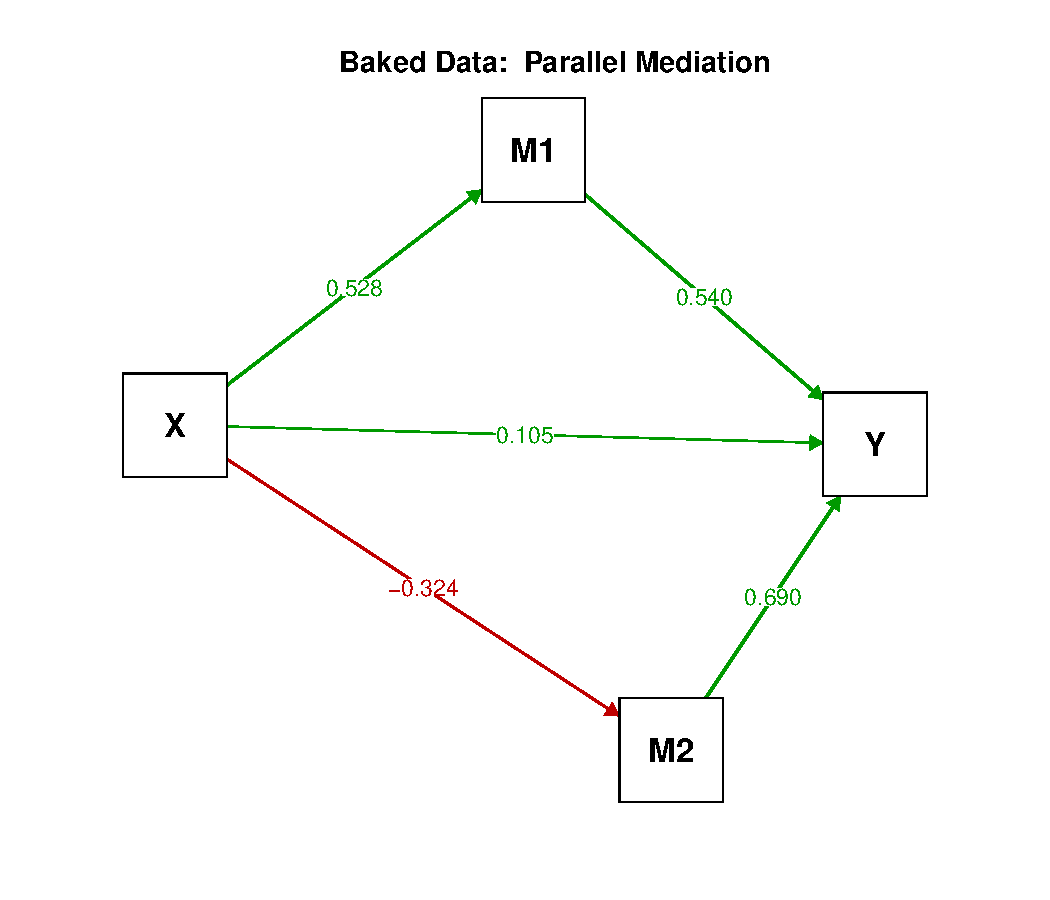
\includegraphics{06-ComplexMed_files/figure-latex/Fake Data Simple Plot-1.pdf}

There are a number of ways to tabalize the data. You might be surprised to learn that a number of articles that analyze mediating effects focus their presentation on those values and not the traditional intercepts and B weights. This is the approach I have taken in this chapter.

\textbf{Table 1 }

\begin{longtable}[]{@{}
  >{\raggedright\arraybackslash}p{(\columnwidth - 0\tabcolsep) * \real{1.0000}}@{}}
\toprule\noalign{}
\begin{minipage}[b]{\linewidth}\raggedright
Model Coefficients Assessing M1 and M2 as Parallel Mediators Between X and Y
\end{minipage} \\
\midrule\noalign{}
\endhead
\bottomrule\noalign{}
\endlastfoot
\end{longtable}

\begin{longtable}[]{@{}
  >{\centering\arraybackslash}p{(\columnwidth - 18\tabcolsep) * \real{0.0690}}
  >{\centering\arraybackslash}p{(\columnwidth - 18\tabcolsep) * \real{0.0345}}
  >{\centering\arraybackslash}p{(\columnwidth - 18\tabcolsep) * \real{0.0345}}
  >{\centering\arraybackslash}p{(\columnwidth - 18\tabcolsep) * \real{0.0345}}
  >{\centering\arraybackslash}p{(\columnwidth - 18\tabcolsep) * \real{0.0460}}
  >{\centering\arraybackslash}p{(\columnwidth - 18\tabcolsep) * \real{0.2989}}
  >{\centering\arraybackslash}p{(\columnwidth - 18\tabcolsep) * \real{0.0345}}
  >{\centering\arraybackslash}p{(\columnwidth - 18\tabcolsep) * \real{0.1379}}
  >{\centering\arraybackslash}p{(\columnwidth - 18\tabcolsep) * \real{0.1609}}
  >{\centering\arraybackslash}p{(\columnwidth - 18\tabcolsep) * \real{0.1494}}@{}}
\toprule\noalign{}
\endhead
\bottomrule\noalign{}
\endlastfoot
IV & & M & & DV & \(B\) for \emph{a} and \emph{b} paths & & \(B\) & \(SE\) & \(p\) \\
X & --\textgreater{} & M1 & --\textgreater{} & DV & (0.528) X (0.540) & = & 0.285 & 0.086 & 0.001 \\
X & --\textgreater{} & M2 & --\textgreater{} & DV & (-0.324) X (0.690) & = & -0.224 & 0.085 & 0.008 \\
\end{longtable}

\begin{longtable}[]{@{}
  >{\centering\arraybackslash}p{(\columnwidth - 6\tabcolsep) * \real{0.5806}}
  >{\centering\arraybackslash}p{(\columnwidth - 6\tabcolsep) * \real{0.1290}}
  >{\centering\arraybackslash}p{(\columnwidth - 6\tabcolsep) * \real{0.1505}}
  >{\centering\arraybackslash}p{(\columnwidth - 6\tabcolsep) * \real{0.1398}}@{}}
\toprule\noalign{}
\endhead
\bottomrule\noalign{}
\endlastfoot
& \(B\) & \(SE\) & \(p\) \\
Total indirect effect & 0.061 & 0.116 & 0.598 \\
Total effect of X on Y (c path) & 0.167 & 0.160 & 0.297 \\
Direct effect of X on Y (c') & 0.105 & 0.130 & 0.130 \\
\end{longtable}

\begin{longtable}[]{@{}
  >{\raggedright\arraybackslash}p{(\columnwidth - 0\tabcolsep) * \real{1.0000}}@{}}
\toprule\noalign{}
\endhead
\bottomrule\noalign{}
\endlastfoot
\end{longtable}

\emph{Note}. X =definition; M1 = definition; M2 = definition; Y = definition. The significance of the indirect effects was calculated with bias-corrected confidence intervals (.95) bootstrap analysis.

\hypertarget{apa-style-writeup}{%
\subsubsection{APA Style Writeup}\label{apa-style-writeup}}

A model of parallel multiple mediation was analyzed examining the degree to which importance of M1 and M2 mediated the relation of X on Y. Hayes \citeyearpar{hayes_introduction_2018} recommended this strategy over simple mediation models because it allows for all mediators to be examined, simultaneously. The resultant direct and indirect values for each path account for other mediation paths. Using the \emph{lavaan (v. 0.6-7)} package in R, coefficients for specific indirect, total indirect, direct, and total were computed. Path coefficients refer to regression weights, or slopes, of the expected changes in the dependent variable given a unit change in the independent variables.

Results (depicted in Figure 1 and presented in Table 2) suggest that of the variance in Y is accounted for by the model. While each of the specific indirect effects (X through M1 and M2, respectively) were statistically significant, the total indirect effect (i.e., the sum of the specific indirect effects was not. This is likely because the indirect effect passing through M1 was positive in valence and the indirect effect passing through M2 was negative; hence, they ``cancelled each other out.'' A pairwise comparison of the specific indirect effects indicated that the strength of the effects were statistically significantly different from each other (\(B\) = 0.509, \(p\) = 0.000). This means that the indirect effect passing through M1 was statistically stronger than the indirect effect passing through M2.

Let's turn now to the research vignette and work an example with simulated data from that example. Because the research vignette use an entirely new set of output I will either restart R or clear my environment so that there are a few less objects ``in the way.''

\hypertarget{research-vignette-5}{%
\subsection{Research Vignette}\label{research-vignette-5}}

The research vignette comes from the Lewis, Williams, Peppers, and Gadson's \citeyearpar{lewis_applying_2017} study titled, ``Applying Intersectionality to Explore the Relations Between Gendered Racism and Health Among Black Women.'' The study was published in the Journal of Counseling Psychology. Participants were 231 Black women who completed an online survey.

Variables used in the study included:

\begin{itemize}
\item
  \textbf{GRMS}: Gendered Racial Microaggressions Scale \citep{lewis_construction_2015} is a 26-item scale that assesses the frequency of nonverbal, verbal, and behavioral negative racial and gender slights experienced by Black women. Scaling is along six points ranging from 0 (never) to 5 (once a week or more). Higher scores indicate a greater frequency of gendered racial microaggressions. An example item is, ``Someone has made a sexually inappropriate comment about my butt, hips, or thighs.''
\item
  \textbf{MntlHlth} and \textbf{PhysHlth}: Short Form Health Survey - Version 2 \citep{ware_comparison_1995} is a 12-item scale used to report self-reported mental (six items) and physical health (six items). Higher scores indicate higher mental health (e.g., little or no psychological ldistress) and physical health (e.g., little or no reported symptoms in physical functioning). An example of an item assessing mental health was, ``How much of the time during the last 4 weeks have you felt calm and peaceful?''; an example of a physical health item was, ``During the past 4 weeks, how much did pain interfere with your normal work?''
\item
  \textbf{Sprtlty}, \textbf{SocSup}, \textbf{Engmgt}, and \textbf{DisEngmt} are four subscales from the Brief Coping with Problems Experienced Inventory \citep{carver_you_1997}. The 28 items on this scale are presented on a 4-point scale ranging from 1 (\emph{I usually do not do this at all}) to 4(\emph{I usually do this a lot}). Higher scores indicate a respondents' tendency to engage in a particular strategy. Instructions were modified to ask how the female participants responded to recent experiences of racism and sexism as Black women. The four subscales included spirituality (religion, acceptance, planning), interconnectedness/social support (vent emotions, emotional support,instrumental social support), problem-oriented/engagement coping (active coping, humor, positive reinterpretation/positive reframing), and disengagement coping (behavioral disengagement, substance abuse, denial, self-blame, self-distraction).
\item
  \textbf{GRIcntlty}: The Multidimensional Inventory of Black Identity Centrality subscale \citep{sellers_multidimensional_nodate} was modified to measure the intersection of racial and gender identity centrality. The scale included 10 items scaled from 1 (\emph{strongly disagree}) to 7 (\emph{strongly agree}). An example item was, ``Being a \emph{Black woman} is important to my self-image.'' Higher scores indicated higher levels of gendered racial identity centrality.
\end{itemize}

\hypertarget{data-simulation-1}{%
\subsubsection{Data Simulation}\label{data-simulation-1}}

Simulating the data:

\begin{Shaded}
\begin{Highlighting}[]
\CommentTok{\#Entering the intercorrelations, means, and standard deviations from the journal article}
\NormalTok{mu }\OtherTok{\textless{}{-}} \FunctionTok{c}\NormalTok{(}\FloatTok{1.99}\NormalTok{, }\FloatTok{2.82}\NormalTok{, }\FloatTok{2.48}\NormalTok{, }\FloatTok{2.32}\NormalTok{, }\FloatTok{1.75}\NormalTok{, }\FloatTok{5.71}\NormalTok{, }\FloatTok{21.37}\NormalTok{, }\FloatTok{21.07}\NormalTok{)}
\NormalTok{sd }\OtherTok{\textless{}{-}} \FunctionTok{c}\NormalTok{(.}\DecValTok{90}\NormalTok{, .}\DecValTok{70}\NormalTok{, .}\DecValTok{81}\NormalTok{, .}\DecValTok{61}\NormalTok{, .}\DecValTok{53}\NormalTok{, }\FloatTok{1.03}\NormalTok{, }\FloatTok{3.83}\NormalTok{, }\FloatTok{4.66}\NormalTok{)}
\NormalTok{r\_mat }\OtherTok{\textless{}{-}} \FunctionTok{matrix}\NormalTok{ (}\FunctionTok{c}\NormalTok{(}\DecValTok{1}\NormalTok{, .}\DecValTok{20}\NormalTok{, .}\DecValTok{28}\NormalTok{, .}\DecValTok{30}\NormalTok{, .}\DecValTok{41}\NormalTok{, .}\DecValTok{19}\NormalTok{, }\SpecialCharTok{{-}}\NormalTok{.}\DecValTok{32}\NormalTok{, }\SpecialCharTok{{-}}\NormalTok{.}\DecValTok{18}\NormalTok{,}
\NormalTok{        .}\DecValTok{20}\NormalTok{, }\DecValTok{1}\NormalTok{, .}\DecValTok{49}\NormalTok{, .}\DecValTok{57}\NormalTok{, .}\DecValTok{22}\NormalTok{, .}\DecValTok{13}\NormalTok{, }\SpecialCharTok{{-}}\NormalTok{.}\DecValTok{06}\NormalTok{, }\SpecialCharTok{{-}}\NormalTok{.}\DecValTok{13}\NormalTok{,}
\NormalTok{        .}\DecValTok{28}\NormalTok{, .}\DecValTok{49}\NormalTok{, }\DecValTok{1}\NormalTok{, .}\DecValTok{46}\NormalTok{, .}\DecValTok{26}\NormalTok{, .}\DecValTok{38}\NormalTok{, }\SpecialCharTok{{-}}\NormalTok{.}\DecValTok{18}\NormalTok{,}\SpecialCharTok{{-}}\NormalTok{.}\DecValTok{08}\NormalTok{, }
\NormalTok{        .}\DecValTok{30}\NormalTok{, .}\DecValTok{57}\NormalTok{, .}\DecValTok{46}\NormalTok{,  }\DecValTok{1}\NormalTok{, .}\DecValTok{37}\NormalTok{, .}\DecValTok{08}\NormalTok{, }\SpecialCharTok{{-}}\NormalTok{.}\DecValTok{14}\NormalTok{, }\SpecialCharTok{{-}}\NormalTok{.}\DecValTok{06}\NormalTok{,}
\NormalTok{        .}\DecValTok{41}\NormalTok{, .}\DecValTok{22}\NormalTok{, .}\DecValTok{26}\NormalTok{, .}\DecValTok{37}\NormalTok{, }\DecValTok{1}\NormalTok{, .}\DecValTok{05}\NormalTok{, }\SpecialCharTok{{-}}\NormalTok{.}\DecValTok{54}\NormalTok{, }\SpecialCharTok{{-}}\NormalTok{.}\DecValTok{28}\NormalTok{, }
\NormalTok{        .}\DecValTok{19}\NormalTok{, .}\DecValTok{13}\NormalTok{, .}\DecValTok{38}\NormalTok{, .}\DecValTok{08}\NormalTok{, .}\DecValTok{05}\NormalTok{, }\DecValTok{1}\NormalTok{, }\SpecialCharTok{{-}}\NormalTok{.}\DecValTok{10}\NormalTok{, .}\DecValTok{14}\NormalTok{, }
        \SpecialCharTok{{-}}\NormalTok{.}\DecValTok{32}\NormalTok{, }\SpecialCharTok{{-}}\NormalTok{.}\DecValTok{06}\NormalTok{, }\SpecialCharTok{{-}}\NormalTok{.}\DecValTok{18}\NormalTok{, }\SpecialCharTok{{-}}\NormalTok{.}\DecValTok{14}\NormalTok{, }\SpecialCharTok{{-}}\NormalTok{.}\DecValTok{54}\NormalTok{, }\SpecialCharTok{{-}}\NormalTok{.}\DecValTok{10}\NormalTok{, }\DecValTok{1}\NormalTok{, .}\DecValTok{47}\NormalTok{,}
        \SpecialCharTok{{-}}\NormalTok{.}\DecValTok{18}\NormalTok{, }\SpecialCharTok{{-}}\NormalTok{.}\DecValTok{13}\NormalTok{, }\SpecialCharTok{{-}}\NormalTok{.}\DecValTok{08}\NormalTok{, }\SpecialCharTok{{-}}\NormalTok{.}\DecValTok{06}\NormalTok{, }\SpecialCharTok{{-}}\NormalTok{.}\DecValTok{28}\NormalTok{, .}\DecValTok{14}\NormalTok{, .}\DecValTok{47}\NormalTok{, }\DecValTok{1}\NormalTok{), }\AttributeTok{ncol =} \DecValTok{8}\NormalTok{)}
\CommentTok{\#Creating a covariance matrix}

\NormalTok{cov\_mat }\OtherTok{\textless{}{-}}\NormalTok{ sd }\SpecialCharTok{\%*\%} \FunctionTok{t}\NormalTok{(sd) }\SpecialCharTok{*}\NormalTok{ r\_mat}
\NormalTok{cov\_mat}
\end{Highlighting}
\end{Shaded}

\begin{verbatim}
##          [,1]     [,2]      [,3]      [,4]      [,5]      [,6]      [,7]
## [1,]  0.81000  0.12600  0.204120  0.164700  0.195570  0.176130 -1.103040
## [2,]  0.12600  0.49000  0.277830  0.243390  0.081620  0.093730 -0.160860
## [3,]  0.20412  0.27783  0.656100  0.227286  0.111618  0.317034 -0.558414
## [4,]  0.16470  0.24339  0.227286  0.372100  0.119621  0.050264 -0.327082
## [5,]  0.19557  0.08162  0.111618  0.119621  0.280900  0.027295 -1.096146
## [6,]  0.17613  0.09373  0.317034  0.050264  0.027295  1.060900 -0.394490
## [7,] -1.10304 -0.16086 -0.558414 -0.327082 -1.096146 -0.394490 14.668900
## [8,] -0.75492 -0.42406 -0.301968 -0.170556 -0.691544  0.671972  8.388466
##           [,8]
## [1,] -0.754920
## [2,] -0.424060
## [3,] -0.301968
## [4,] -0.170556
## [5,] -0.691544
## [6,]  0.671972
## [7,]  8.388466
## [8,] 21.715600
\end{verbatim}

\begin{Shaded}
\begin{Highlighting}[]
\CommentTok{\#Set random seed so that the following matrix always gets the same results.}
\FunctionTok{set.seed}\NormalTok{(}\DecValTok{210403}\NormalTok{)}
\FunctionTok{library}\NormalTok{(MASS)}
\end{Highlighting}
\end{Shaded}

\begin{verbatim}
## 
## Attaching package: 'MASS'
\end{verbatim}

\begin{verbatim}
## The following object is masked from 'package:formattable':
## 
##     area
\end{verbatim}

\begin{Shaded}
\begin{Highlighting}[]
\NormalTok{Lewis\_df }\OtherTok{\textless{}{-}} \FunctionTok{mvrnorm}\NormalTok{(}\AttributeTok{n =} \DecValTok{212}\NormalTok{, }\AttributeTok{mu=}\NormalTok{mu, }\AttributeTok{Sigma =}\NormalTok{ cov\_mat, }\AttributeTok{empirical =} \ConstantTok{TRUE}\NormalTok{)}
\FunctionTok{colMeans}\NormalTok{(Lewis\_df)}
\end{Highlighting}
\end{Shaded}

\begin{verbatim}
## [1]  1.99  2.82  2.48  2.32  1.75  5.71 21.37 21.07
\end{verbatim}

\begin{Shaded}
\begin{Highlighting}[]
\CommentTok{\#Checking our work against the original correlation matrix}
\FunctionTok{cor}\NormalTok{(Lewis\_df)}
\end{Highlighting}
\end{Shaded}

\begin{verbatim}
##       [,1]  [,2]  [,3]  [,4]  [,5]  [,6]  [,7]  [,8]
## [1,]  1.00  0.20  0.28  0.30  0.41  0.19 -0.32 -0.18
## [2,]  0.20  1.00  0.49  0.57  0.22  0.13 -0.06 -0.13
## [3,]  0.28  0.49  1.00  0.46  0.26  0.38 -0.18 -0.08
## [4,]  0.30  0.57  0.46  1.00  0.37  0.08 -0.14 -0.06
## [5,]  0.41  0.22  0.26  0.37  1.00  0.05 -0.54 -0.28
## [6,]  0.19  0.13  0.38  0.08  0.05  1.00 -0.10  0.14
## [7,] -0.32 -0.06 -0.18 -0.14 -0.54 -0.10  1.00  0.47
## [8,] -0.18 -0.13 -0.08 -0.06 -0.28  0.14  0.47  1.00
\end{verbatim}

Rename the variables

\begin{Shaded}
\begin{Highlighting}[]
\FunctionTok{as.data.frame}\NormalTok{(Lewis\_df, }\AttributeTok{row.names =} \ConstantTok{NULL}\NormalTok{, }\AttributeTok{optional =} \ConstantTok{FALSE}\NormalTok{, }\AttributeTok{make.names =} \ConstantTok{TRUE}\NormalTok{)}
\FunctionTok{library}\NormalTok{(tidyverse)}
\NormalTok{Lewis\_df }\OtherTok{\textless{}{-}}\NormalTok{ Lewis\_df}\SpecialCharTok{\%\textgreater{}\%}
\NormalTok{  as.data.frame }\SpecialCharTok{\%\textgreater{}\%}
  \FunctionTok{rename}\NormalTok{(}\AttributeTok{GRMS =}\NormalTok{ V1, }\AttributeTok{Sprtlty =}\NormalTok{ V2, }\AttributeTok{SocSup =}\NormalTok{ V3, }\AttributeTok{Engmt =}\NormalTok{ V4, }\AttributeTok{DisEngmt =}\NormalTok{ V5, }\AttributeTok{GRIcntlty =}\NormalTok{ V6, }\AttributeTok{MtnlHlth =}\NormalTok{ V7, }\AttributeTok{PhysHlth =}\NormalTok{ V8)}
\end{Highlighting}
\end{Shaded}

\begin{Shaded}
\begin{Highlighting}[]
\FunctionTok{head}\NormalTok{(Lewis\_df)}
\end{Highlighting}
\end{Shaded}

\begin{verbatim}
##        GRMS  Sprtlty   SocSup    Engmt DisEngmt GRIcntlty MtnlHlth PhysHlth
## 1 0.7792361 2.628957 1.758948 1.691459 1.062341  5.533258 22.70042 19.42231
## 2 1.5729406 1.943789 1.101567 2.446707 1.885076  5.806530 22.67086 22.25516
## 3 1.9586843 3.039406 1.591625 2.428866 1.635518  5.166721 19.06958 23.23199
## 4 0.6532324 2.624590 1.039778 1.495290 1.506393  4.276244 23.90836 18.74549
## 5 2.8280150 3.242341 2.202956 1.553723 1.024422  5.730293 22.86224 18.80227
## 6 1.2809196 3.052410 4.097964 2.727955 1.565009  8.474002 19.13631 24.48153
\end{verbatim}

\hypertarget{quick-descriptives}{%
\subsubsection{Quick Descriptives}\label{quick-descriptives}}

Of course it is is a good idea to examine our data ahead of time. While we won't take time to do a thorough analysis, we can at least take a peek.

\begin{Shaded}
\begin{Highlighting}[]
\FunctionTok{library}\NormalTok{(psych)}
\end{Highlighting}
\end{Shaded}

\begin{verbatim}
## 
## Attaching package: 'psych'
\end{verbatim}

\begin{verbatim}
## The following objects are masked from 'package:ggplot2':
## 
##     %+%, alpha
\end{verbatim}

\begin{verbatim}
## The following object is masked from 'package:lavaan':
## 
##     cor2cov
\end{verbatim}

\begin{Shaded}
\begin{Highlighting}[]
\NormalTok{psych}\SpecialCharTok{::}\FunctionTok{describe}\NormalTok{(Lewis\_df)}
\end{Highlighting}
\end{Shaded}

\begin{verbatim}
##           vars   n  mean   sd median trimmed  mad   min   max range  skew
## GRMS         1 212  1.99 0.90   2.01    2.00 0.93 -0.75  4.24  4.99 -0.12
## Sprtlty      2 212  2.82 0.70   2.75    2.82 0.65  0.46  4.68  4.23 -0.06
## SocSup       3 212  2.48 0.81   2.47    2.46 0.77 -0.32  4.68  5.00  0.11
## Engmt        4 212  2.32 0.61   2.33    2.32 0.57  0.37  4.08  3.71 -0.02
## DisEngmt     5 212  1.75 0.53   1.75    1.75 0.55  0.58  3.00  2.42 -0.04
## GRIcntlty    6 212  5.71 1.03   5.67    5.68 1.00  3.08  9.40  6.32  0.32
## MtnlHlth     7 212 21.37 3.83  21.60   21.46 4.29 11.65 31.90 20.25 -0.15
## PhysHlth     8 212 21.07 4.66  20.79   21.03 4.68  8.43 33.71 25.28  0.07
##           kurtosis   se
## GRMS         -0.14 0.06
## Sprtlty       0.34 0.05
## SocSup        0.41 0.06
## Engmt         0.22 0.04
## DisEngmt     -0.64 0.04
## GRIcntlty     0.36 0.07
## MtnlHlth     -0.54 0.26
## PhysHlth     -0.18 0.32
\end{verbatim}

We note that our means and standard deviations map exactly onto those in the article. Because we asked for a normal distribution, we do not violate any of the assumptions related to univariate normality; our skew and kurtosis are well within the limits.

The pairs panel from the \emph{psych} package is an efficient way to see

\begin{itemize}
\tightlist
\item
  the distribution of each variable with a normal curve superimposed (on the diagonal)
\item
  the value of the bivariate correlation (upper diagonal)
\item
  a scatterplot with a regression line between each pair of variables (lower diagonal)
\end{itemize}

\begin{Shaded}
\begin{Highlighting}[]
\NormalTok{psych}\SpecialCharTok{::}\FunctionTok{pairs.panels}\NormalTok{(Lewis\_df)}
\end{Highlighting}
\end{Shaded}

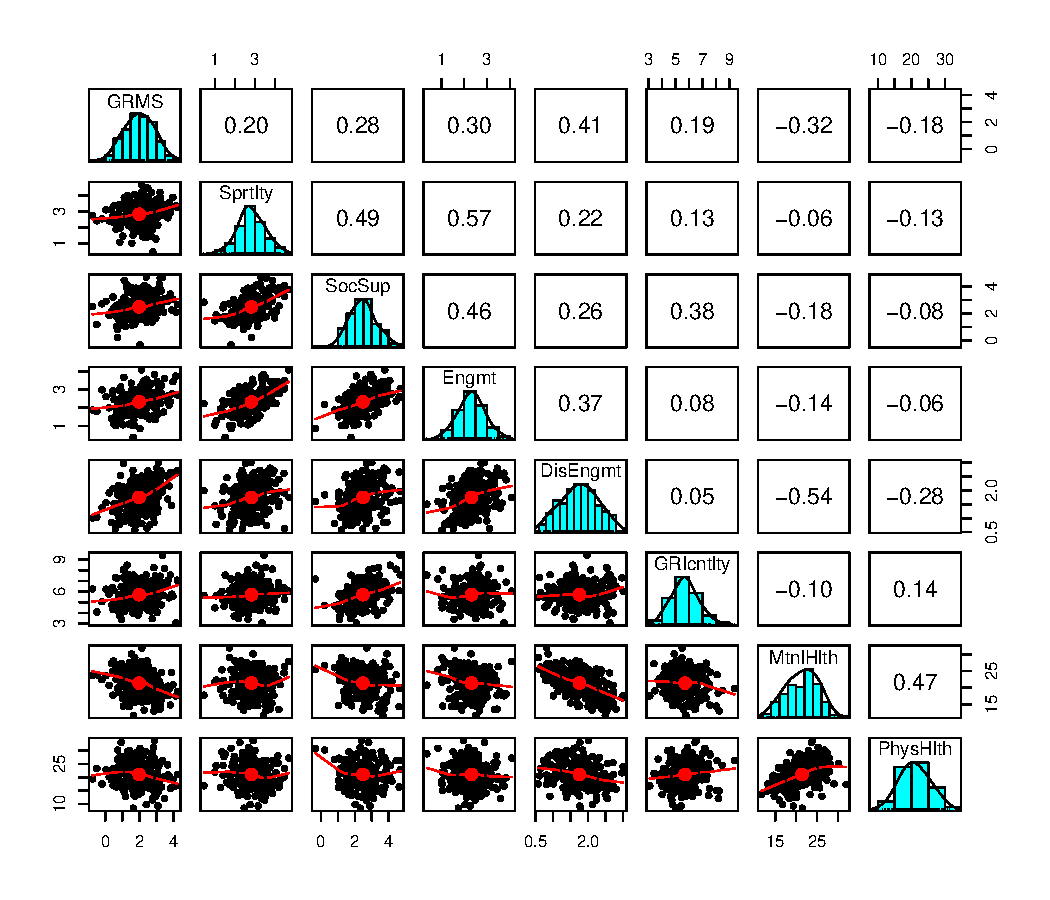
\includegraphics{06-ComplexMed_files/figure-latex/unnamed-chunk-4-1.pdf}

The Lewis et al.~article \citeyearpar{lewis_applying_2017} reports four mediation analyses, each repeated for mental and physical outcomes. Thus, their write-up reports eight simple mediation models. Graphically, this is efficiently represented in a figure that looks like parallel mediation. Note that the figure is reporting standardized estimates. In Hayes' \citeyearpar{hayes_introduction_2018} we have been using raw, \(B\) weights. However, the standardized weights are reported in the output.

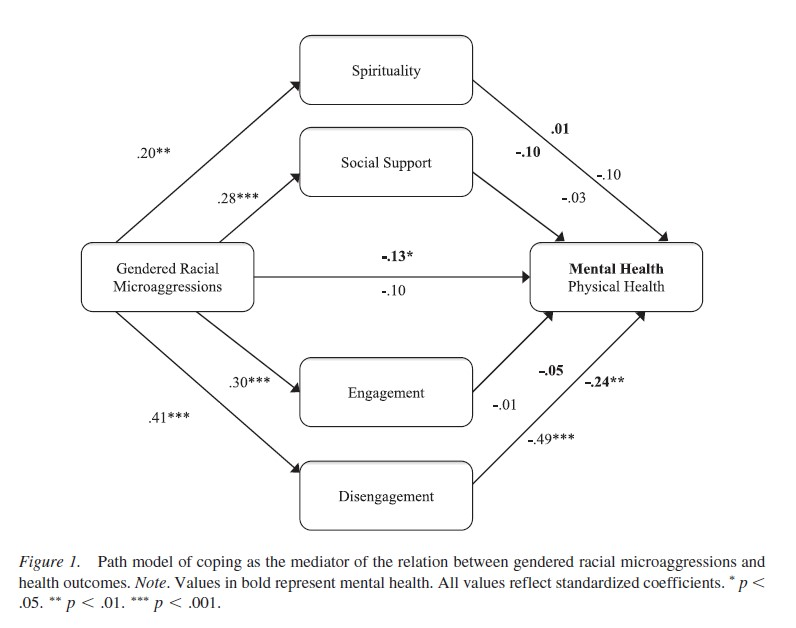
\includegraphics{images/CompMed/LewisMedFig.jpg} Because the figure looked like a parallel mediation, it made sense to me that we could try this in our research vignette. In the chapter on conditional process analysis, we will work the moderated mediation as they have done. Below is the model we will work. Specifically, we will evaluate whether gendered racial microaggressions impact mental health separately, thorough mediated paths of engagement and disengagement. We will also be able to see if the strength of those mediated paths are statistically, significantly, different from each other.

\begin{figure}
\centering
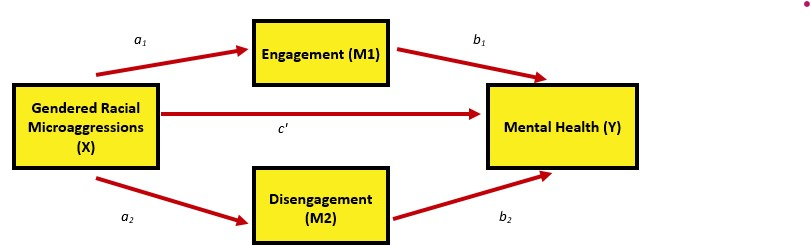
\includegraphics{images/CompMed/LewisParaMed.jpg}
\caption{An image of the parallel mediation we will work}
\end{figure}

\hypertarget{specifying-the-lavaan-model}{%
\subsubsection{\texorpdfstring{Specifying the \emph{lavaan} model}{Specifying the lavaan model}}\label{specifying-the-lavaan-model}}

We can use the guidelines above to specify our model and then request summaries of the fit indices and parameter estimates.

\begin{Shaded}
\begin{Highlighting}[]
\FunctionTok{set.seed}\NormalTok{(}\DecValTok{210403}\NormalTok{)}
\FunctionTok{library}\NormalTok{(lavaan)}

\NormalTok{parallel\_Lewis }\OtherTok{\textless{}{-}} \StringTok{\textquotesingle{}}
\StringTok{    MtnlHlth \textasciitilde{} b1*Engmt + b2*DisEngmt + c\_p*GRMS}
\StringTok{    Engmt \textasciitilde{} a1*GRMS    }
\StringTok{    DisEngmt \textasciitilde{} a2*GRMS}
\StringTok{    indirect1 := a1 * b1}
\StringTok{    indirect2 := a2 * b2}
\StringTok{    contrast := indirect1 {-} indirect2}
\StringTok{    total\_indirects := indirect1 + indirect2}
\StringTok{    total\_c := c\_p + (indirect1) + (indirect2)}
\StringTok{    direct := c\_p}
\StringTok{\textquotesingle{}}
\NormalTok{para\_Lewis\_fit }\OtherTok{\textless{}{-}} \FunctionTok{sem}\NormalTok{(parallel\_Lewis, }\AttributeTok{data =}\NormalTok{ Lewis\_df, }\AttributeTok{se =} \StringTok{"bootstrap"}\NormalTok{, }\AttributeTok{bootstrap =} \DecValTok{1000}\NormalTok{, }\AttributeTok{missing =} \StringTok{\textquotesingle{}fiml\textquotesingle{}}\NormalTok{) }\CommentTok{\#holds the "whole" result}
\NormalTok{pLewis\_sum }\OtherTok{\textless{}{-}} \FunctionTok{summary}\NormalTok{(para\_Lewis\_fit , }\AttributeTok{standardized =} \ConstantTok{TRUE}\NormalTok{, }\AttributeTok{rsq=}\NormalTok{T, }\AttributeTok{fit=}\ConstantTok{TRUE}\NormalTok{, }\AttributeTok{ci=}\ConstantTok{TRUE}\NormalTok{) }\CommentTok{\#today, we really only need the R{-}squared from here    }
\NormalTok{pLewis\_ParEsts }\OtherTok{\textless{}{-}} \FunctionTok{parameterEstimates}\NormalTok{(para\_Lewis\_fit, }\AttributeTok{boot.ci.type =} \StringTok{"bca.simple"}\NormalTok{, }\AttributeTok{standardized=}\ConstantTok{TRUE}\NormalTok{) }\CommentTok{\#provides our estimates, se, p values for all the elements we specified}
\end{Highlighting}
\end{Shaded}

\begin{Shaded}
\begin{Highlighting}[]
\NormalTok{pLewis\_sum}
\end{Highlighting}
\end{Shaded}

\begin{verbatim}
## lavaan 0.6.16 ended normally after 1 iteration
## 
##   Estimator                                         ML
##   Optimization method                           NLMINB
##   Number of model parameters                        11
## 
##   Number of observations                           212
##   Number of missing patterns                         1
## 
## Model Test User Model:
##                                                       
##   Test statistic                                17.813
##   Degrees of freedom                                 1
##   P-value (Chi-square)                           0.000
## 
## Model Test Baseline Model:
## 
##   Test statistic                               155.625
##   Degrees of freedom                                 6
##   P-value                                        0.000
## 
## User Model versus Baseline Model:
## 
##   Comparative Fit Index (CFI)                    0.888
##   Tucker-Lewis Index (TLI)                       0.326
##                                                       
##   Robust Comparative Fit Index (CFI)             0.888
##   Robust Tucker-Lewis Index (TLI)                0.326
## 
## Loglikelihood and Information Criteria:
## 
##   Loglikelihood user model (H0)               -877.337
##   Loglikelihood unrestricted model (H1)       -868.431
##                                                       
##   Akaike (AIC)                                1776.675
##   Bayesian (BIC)                              1813.597
##   Sample-size adjusted Bayesian (SABIC)       1778.742
## 
## Root Mean Square Error of Approximation:
## 
##   RMSEA                                          0.282
##   90 Percent confidence interval - lower         0.177
##   90 Percent confidence interval - upper         0.403
##   P-value H_0: RMSEA <= 0.050                    0.000
##   P-value H_0: RMSEA >= 0.080                    0.999
##                                                       
##   Robust RMSEA                                   0.282
##   90 Percent confidence interval - lower         0.177
##   90 Percent confidence interval - upper         0.403
##   P-value H_0: Robust RMSEA <= 0.050             0.000
##   P-value H_0: Robust RMSEA >= 0.080             0.999
## 
## Standardized Root Mean Square Residual:
## 
##   SRMR                                           0.075
## 
## Parameter Estimates:
## 
##   Standard errors                            Bootstrap
##   Number of requested bootstrap draws             1000
##   Number of successful bootstrap draws            1000
## 
## Regressions:
##                    Estimate  Std.Err  z-value  P(>|z|) ci.lower ci.upper
##   MtnlHlth ~                                                            
##     Engmt     (b1)    0.581    0.431    1.346    0.178   -0.287    1.447
##     DisEngmt  (b2)   -3.750    0.471   -7.954    0.000   -4.670   -2.851
##     GRMS     (c_p)   -0.575    0.243   -2.363    0.018   -1.071   -0.126
##   Engmt ~                                                               
##     GRMS      (a1)    0.203    0.044    4.584    0.000    0.116    0.292
##   DisEngmt ~                                                            
##     GRMS      (a2)    0.241    0.037    6.570    0.000    0.169    0.312
##    Std.lv  Std.all
##                   
##     0.581    0.091
##    -3.750   -0.513
##    -0.575   -0.133
##                   
##     0.203    0.300
##                   
##     0.241    0.410
## 
## Intercepts:
##                    Estimate  Std.Err  z-value  P(>|z|) ci.lower ci.upper
##    .MtnlHlth         27.728    1.027   27.004    0.000   25.525   29.753
##    .Engmt             1.915    0.100   19.140    0.000    1.720    2.110
##    .DisEngmt          1.270    0.080   15.877    0.000    1.106    1.423
##    Std.lv  Std.all
##    27.728    7.172
##     1.915    3.147
##     1.270    2.401
## 
## Variances:
##                    Estimate  Std.Err  z-value  P(>|z|) ci.lower ci.upper
##    .MtnlHlth         10.067    0.846   11.895    0.000    8.249   11.477
##    .Engmt             0.337    0.035    9.718    0.000    0.270    0.402
##    .DisEngmt          0.233    0.021   10.927    0.000    0.190    0.275
##    Std.lv  Std.all
##    10.067    0.674
##     0.337    0.910
##     0.233    0.832
## 
## R-Square:
##                    Estimate
##     MtnlHlth          0.326
##     Engmt             0.090
##     DisEngmt          0.168
## 
## Defined Parameters:
##                    Estimate  Std.Err  z-value  P(>|z|) ci.lower ci.upper
##     indirect1         0.118    0.095    1.249    0.212   -0.062    0.310
##     indirect2        -0.905    0.182   -4.974    0.000   -1.305   -0.574
##     contrast          1.023    0.224    4.578    0.000    0.618    1.491
##     total_indircts   -0.787    0.185   -4.259    0.000   -1.152   -0.440
##     total_c          -1.362    0.253   -5.392    0.000   -1.841   -0.864
##     direct           -0.575    0.243   -2.362    0.018   -1.071   -0.126
##    Std.lv  Std.all
##     0.118    0.027
##    -0.905   -0.210
##     1.023    0.238
##    -0.787   -0.183
##    -1.362   -0.316
##    -0.575   -0.133
\end{verbatim}

\begin{Shaded}
\begin{Highlighting}[]
\NormalTok{pLewis\_ParEsts}
\end{Highlighting}
\end{Shaded}

\begin{verbatim}
##                lhs op                         rhs           label    est    se
## 1         MtnlHlth  ~                       Engmt              b1  0.581 0.431
## 2         MtnlHlth  ~                    DisEngmt              b2 -3.750 0.471
## 3         MtnlHlth  ~                        GRMS             c_p -0.575 0.243
## 4            Engmt  ~                        GRMS              a1  0.203 0.044
## 5         DisEngmt  ~                        GRMS              a2  0.241 0.037
## 6         MtnlHlth ~~                    MtnlHlth                 10.067 0.846
## 7            Engmt ~~                       Engmt                  0.337 0.035
## 8         DisEngmt ~~                    DisEngmt                  0.233 0.021
## 9             GRMS ~~                        GRMS                  0.806 0.000
## 10        MtnlHlth ~1                                             27.728 1.027
## 11           Engmt ~1                                              1.915 0.100
## 12        DisEngmt ~1                                              1.270 0.080
## 13            GRMS ~1                                              1.990 0.000
## 14       indirect1 :=                       a1*b1       indirect1  0.118 0.095
## 15       indirect2 :=                       a2*b2       indirect2 -0.905 0.182
## 16        contrast :=         indirect1-indirect2        contrast  1.023 0.224
## 17 total_indirects :=         indirect1+indirect2 total_indirects -0.787 0.185
## 18         total_c := c_p+(indirect1)+(indirect2)         total_c -1.362 0.253
## 19          direct :=                         c_p          direct -0.575 0.243
##         z pvalue ci.lower ci.upper std.lv std.all std.nox
## 1   1.346  0.178   -0.339    1.354  0.581   0.091   0.091
## 2  -7.954  0.000   -4.703   -2.892 -3.750  -0.513  -0.513
## 3  -2.363  0.018   -1.047   -0.099 -0.575  -0.133  -0.149
## 4   4.584  0.000    0.116    0.292  0.203   0.300   0.334
## 5   6.570  0.000    0.170    0.313  0.241   0.410   0.457
## 6  11.895  0.000    8.599   11.773 10.067   0.674   0.674
## 7   9.718  0.000    0.279    0.414  0.337   0.910   0.910
## 8  10.927  0.000    0.199    0.286  0.233   0.832   0.832
## 9      NA     NA    0.806    0.806  0.806   1.000   0.806
## 10 27.004  0.000   25.599   29.794 27.728   7.172   7.172
## 11 19.140  0.000    1.719    2.109  1.915   3.147   3.147
## 12 15.877  0.000    1.094    1.416  1.270   2.401   2.401
## 13     NA     NA    1.990    1.990  1.990   2.216   1.990
## 14  1.249  0.212   -0.061    0.311  0.118   0.027   0.031
## 15 -4.974  0.000   -1.370   -0.602 -0.905  -0.210  -0.234
## 16  4.578  0.000    0.650    1.561  1.023   0.238   0.265
## 17 -4.259  0.000   -1.198   -0.471 -0.787  -0.183  -0.204
## 18 -5.392  0.000   -1.873   -0.891 -1.362  -0.316  -0.352
## 19 -2.362  0.018   -1.047   -0.099 -0.575  -0.133  -0.149
\end{verbatim}

\hypertarget{figures-and-tables-1}{%
\subsubsection{Figures and Tables}\label{figures-and-tables-1}}

When I interpret the data I first plot it and then create the table. Both processes force me to slow down and work conceptually through and deeply in the data.

\begin{Shaded}
\begin{Highlighting}[]
\FunctionTok{library}\NormalTok{(semPlot)}
\CommentTok{\#note change in layout }
\FunctionTok{semPaths}\NormalTok{(para\_Lewis\_fit, }\CommentTok{\#must identiy the model you want to map}
         \AttributeTok{what =} \StringTok{"est"}\NormalTok{, }\CommentTok{\#"est" plots the estimates, but keeps it greyscale with no fading}
         \CommentTok{\#whatLabels = "stand", \#"stand" changes to standardized values}
         \CommentTok{\#layout = \textquotesingle{}tree\textquotesingle{}, rotation = 2, \#together, puts predictors on left, IVs on right }
         \AttributeTok{layout =} \StringTok{\textquotesingle{}spring\textquotesingle{}}\NormalTok{, }
         \AttributeTok{edge.label.cex =} \FloatTok{1.00}\NormalTok{, }\CommentTok{\#font size of parameter values}
         \CommentTok{\#edge.color = "black", \#overwrites the green/black coloring}
         \AttributeTok{sizeMan=}\DecValTok{10}\NormalTok{, }\CommentTok{\#size of squares/observed/"manifest" variables}
         \AttributeTok{fade=}\ConstantTok{FALSE}\NormalTok{, }\CommentTok{\#if TRUE, there lines are faded such that weaker lines correspond with lower values {-}{-} a cool effect, but tough for journals}
         \AttributeTok{esize=}\DecValTok{2}\NormalTok{, }
         \AttributeTok{asize=}\DecValTok{3}\NormalTok{,}
         \CommentTok{\#label.prop = .5,}
         \AttributeTok{label.font =} \FloatTok{2.5}\NormalTok{, }\CommentTok{\#controls size (I think) of font for labels}
         \AttributeTok{label.scale =} \ConstantTok{TRUE}\NormalTok{, }\CommentTok{\#if false, the labels will not scale to fit inside the nodes}
         \AttributeTok{nDigits =} \DecValTok{3}\NormalTok{, }\CommentTok{\#decimal places (default is 2)}
         \AttributeTok{residuals =} \ConstantTok{FALSE}\NormalTok{,}\CommentTok{\#excludes residuals (and variances) from the path diagram}
         \AttributeTok{nCharNodes =} \DecValTok{0}\NormalTok{, }\CommentTok{\#specifies how many characters to abbreviate variable lables; default is 3.  If 0, uses your entire variable label and adjusts fontsize (which could be a downside)}
         \AttributeTok{intercepts =} \ConstantTok{FALSE}\NormalTok{, }\CommentTok{\#gets rid of those annoying triangles (intercepts) in the path diagram)}
\NormalTok{)}
\FunctionTok{title}\NormalTok{(}\StringTok{"Mental Health from Gendered Racial Microaggressions, Mediated by Engagement and Disengagement Coping"}\NormalTok{)}
\end{Highlighting}
\end{Shaded}

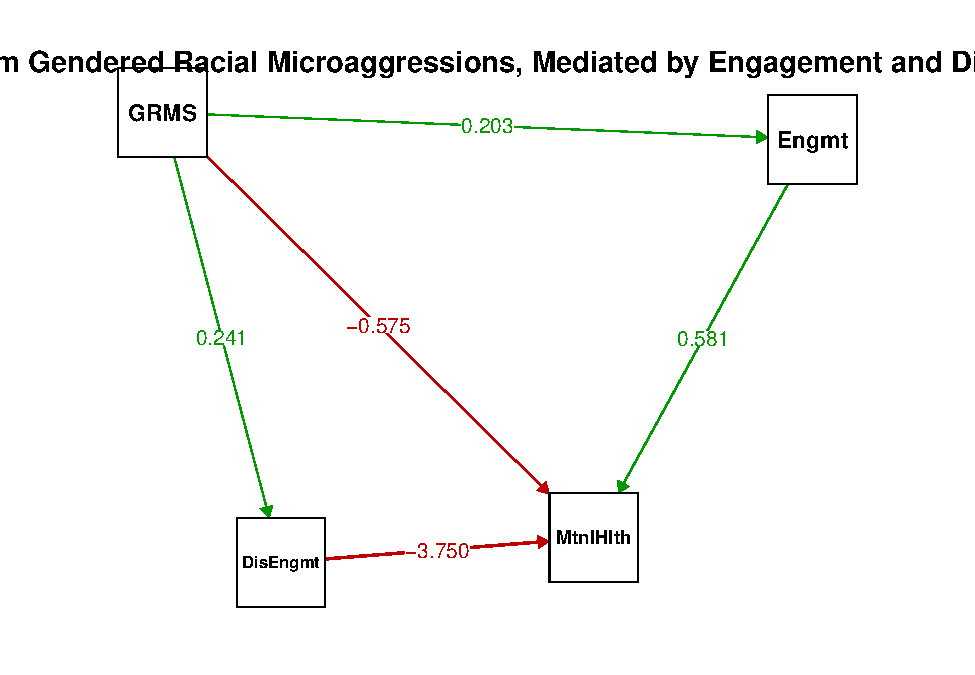
\includegraphics{06-ComplexMed_files/figure-latex/Lewis Parallel model plot-1.pdf}

Now let's make a table.

\textbf{Table 2 }

\begin{longtable}[]{@{}
  >{\raggedright\arraybackslash}p{(\columnwidth - 0\tabcolsep) * \real{1.0000}}@{}}
\toprule\noalign{}
\begin{minipage}[b]{\linewidth}\raggedright
Model Coefficients Assessing Engagement and Disengagement Coping as Parallel Mediators Between Predicting Mental Health from Gendered Racial Microaggressions
\end{minipage} \\
\midrule\noalign{}
\endhead
\bottomrule\noalign{}
\endlastfoot
\end{longtable}

\begin{longtable}[]{@{}
  >{\centering\arraybackslash}p{(\columnwidth - 18\tabcolsep) * \real{0.0600}}
  >{\centering\arraybackslash}p{(\columnwidth - 18\tabcolsep) * \real{0.0300}}
  >{\centering\arraybackslash}p{(\columnwidth - 18\tabcolsep) * \real{0.0900}}
  >{\centering\arraybackslash}p{(\columnwidth - 18\tabcolsep) * \real{0.0300}}
  >{\centering\arraybackslash}p{(\columnwidth - 18\tabcolsep) * \real{0.1000}}
  >{\centering\arraybackslash}p{(\columnwidth - 18\tabcolsep) * \real{0.2500}}
  >{\centering\arraybackslash}p{(\columnwidth - 18\tabcolsep) * \real{0.0300}}
  >{\centering\arraybackslash}p{(\columnwidth - 18\tabcolsep) * \real{0.1200}}
  >{\centering\arraybackslash}p{(\columnwidth - 18\tabcolsep) * \real{0.1500}}
  >{\centering\arraybackslash}p{(\columnwidth - 18\tabcolsep) * \real{0.1400}}@{}}
\toprule\noalign{}
\endhead
\bottomrule\noalign{}
\endlastfoot
IV & & M & & DV & \(B\) for \emph{a} and \emph{b} paths & & \(B\) & \(SE\) & \(p\) \\
GRMS & --\textgreater{} & Engmt & --\textgreater{} & MntlHlth & (0.203) X (0.581) & = & 0.118 & 0.095 & 0.212 \\
GRMS & --\textgreater{} & DisEngmt & --\textgreater{} & MntlHlth & (0.241) X (-3.750) & = & -0.905 & 0.182 & 0.000 \\
\end{longtable}

\begin{longtable}[]{@{}
  >{\centering\arraybackslash}p{(\columnwidth - 6\tabcolsep) * \real{0.6132}}
  >{\centering\arraybackslash}p{(\columnwidth - 6\tabcolsep) * \real{0.1132}}
  >{\centering\arraybackslash}p{(\columnwidth - 6\tabcolsep) * \real{0.1415}}
  >{\centering\arraybackslash}p{(\columnwidth - 6\tabcolsep) * \real{0.1321}}@{}}
\toprule\noalign{}
\endhead
\bottomrule\noalign{}
\endlastfoot
& \(B\) & \(SE\) & \(p\) \\
Total indirect effect & -0.787 & 0.185 & 0.000 \\
Total effect of X on Y (c path) & -1.362 & 0.253 & 0.000 \\
Direct effect of X on Y (c') & -0.575 & 0.243 & 0.243 \\
\end{longtable}

\begin{longtable}[]{@{}
  >{\raggedright\arraybackslash}p{(\columnwidth - 0\tabcolsep) * \real{1.0000}}@{}}
\toprule\noalign{}
\endhead
\bottomrule\noalign{}
\endlastfoot
\end{longtable}

\emph{Note}. IV = gendered racial microaggressions; M1 = engagement coping; M2 = disengagement coping; Y = mental health. The significance of the indirect effects was calculated with bias-corrected confidence intervals (.95) bootstrap analysis.

\begin{itemize}
\tightlist
\item
  The model accounts for of the variance in predicting mental health outcomes.
\item
  The total effect of GRMS on mental health is -1.362 (\(p\) = 0.000) is negative and statistically significant. That is, gendered racial microaggressions have a statistically significant negative effect on mental health.
\item
  The direct effect of GRMS on mental health is -0.575 (\emph{p} = 0.243) is still negative but not statistically significant.

  \begin{itemize}
  \tightlist
  \item
    Using Baron and Kenny's \citeyearpar{baron_moderator-mediator_1986} causal steps logic, the smaller and non-significant direct effect (compared to the total effect) provides helpful, logical support for mediation. According to Hayes \citeyearpar{hayes_introduction_2018} this difference is not necessary. However it is logically helpful.
  \end{itemize}
\item
  Indirect effect \#1 (a1 x b1 or GRMS through engagement coping) is 0.118 (\(p\) = 0.000) and not statistically significant. Looking at the paths we see that \emph{a1} is positive and statistically significant (GRMS leds to increased engagement coping), but the next link, \emph{b1} (engagement to mental health) is not statistically significant.
\item
  Indirect effect \#2 (a2 x b2, or GRMS through disengagement to coping) is -0.905(\(p\) = 0.000). Gendered racial microaggressions lead to greater disengagement (\emph{a1}). In turn, disengagement has negative effects on mental health (\emph{b2})
\item
  The total indirect effect (i.e., sum of M1 and M2) -0.787 (\(p\) = 0.000 ) The sum of all specific indirect effects; statistically significant.
\item
  We look at the contrast to see if the indirect effects statistically significantly different from each other? \(B\) = 1.023, \(p\) = 0.000. They are. This is not surprising since the path mediated by engagement was not statistically significant but the path mediated by disengagement was statistically significant.
\end{itemize}

\begin{Shaded}
\begin{Highlighting}[]
\NormalTok{LewisparaTable }\OtherTok{\textless{}{-}} \FunctionTok{semTable}\NormalTok{(para\_Lewis\_fit, }\AttributeTok{columns =} \FunctionTok{c}\NormalTok{(}\StringTok{"est"}\NormalTok{, }\StringTok{"se"}\NormalTok{, }\StringTok{"p"}\NormalTok{, }\StringTok{"rsquare"}\NormalTok{),  }\AttributeTok{columnLabels =} \FunctionTok{c}\NormalTok{(}\AttributeTok{eststars =} \StringTok{"Estimate"}\NormalTok{), }\AttributeTok{paramSets =} \FunctionTok{c}\NormalTok{(}\StringTok{"composites"}\NormalTok{, }\StringTok{"loadings"}\NormalTok{, }\StringTok{"slopes"}\NormalTok{, }\StringTok{"intercepts"}\NormalTok{, }\StringTok{"residualvariances"}\NormalTok{), }\AttributeTok{file =} \StringTok{"LewisParaTable"}\NormalTok{, }\AttributeTok{type =} \StringTok{"csv"}\NormalTok{, }\AttributeTok{print.results =} \ConstantTok{TRUE}\NormalTok{)}
\end{Highlighting}
\end{Shaded}

\begin{verbatim}
## ,Model,
##  
## ,Estimate,Std. Err.,p,R Square,
## 
## ,Regression Slopes,
##  MtnlHlth,
## 
## Engmt,0.58,0.43,.178,,
## 
## DisEngmt,-3.75,0.47,.000,,
## 
## GRMS,-0.57,0.24,.018,,
## 
##  Engmt,
## 
## GRMS,0.20,0.04,.000,,
## 
##  DisEngmt,
## 
## GRMS,0.24,0.04,.000,,
## 
## ,Intercepts,
## 
## MtnlHlth,27.73,1.03,.000,,
## 
## Engmt,1.92,0.10,.000,,
## 
## DisEngmt,1.27,0.08,.000,,
## 
## GRMS,1.99+,,,,
## 
## ,Residual Variances,
## 
## MtnlHlth,10.07,0.85,.000,,
## 
## Engmt,0.34,0.03,.000,,
## 
## DisEngmt,0.23,0.02,.000,,
## 
## GRMS,0.81+,,,,
## 
## ,Fit Indices,
## 
## chi^2,17.81(1),,.000,,
## 
## CFI,0.89,,,,
## 
## TLI,0.33,,,,
## 
## RMSEA,0.28,,,,
## 
## +Fixed parameter,
## 
## 
## 
## 
\end{verbatim}

\hypertarget{apa-style-writeup-1}{%
\subsubsection{APA Style Writeup}\label{apa-style-writeup-1}}

Hayes \citeyearpar{hayes_introduction_2018} provides helpful guidelines for presenting statistical results. Here is a summary of his recommendations.

\begin{itemize}
\tightlist
\item
  Pack as much statistical info as possible into a table(s) or figure (s).
\item
  Use statistics in the text as punctuation; avoid redundancy in text and table.
\item
  Avoid using abbreviations for variables in the text itself; rather focus on the construct names rather than their shorthand
\item
  Avoid focusing on what you hypothesized (e.g., avoid, ``Results supported/did not support hypothesis A1'') and instead focus on what you found. The reader is more interested in the results, not your forecasts.
\item
  Hayes uses unstandardized metrics. He prefers reporting unstandardized metrics because they map onto the measurement scales used in the study. He believes this is especially important when dichotomous variables are used.
\item
  There is ``no harm'' in reporting hypothesis tests and CIs for the a and b paths, but whether/not these paths are statistically significant does not determine the significance of the indirect effect.
\item
  Be precise with language:
\item
  OK: X exerts an effect on Y directly and/or indirectly through M.
\item
  Not OK: the indirect effect of M\\
\item
  Report direct and indirect effects and their corresponding inferential tests
\item
  Hayes argues that a statistically significant indirect effect is, in fact statistic. He dislikes narration of the Baron and Kenny \citeyearpar{baron_moderator-mediator_1986} process and steps.
\end{itemize}

Here's my attempt to write up the simulated data from the Lewis et al. \citeyearpar{lewis_applying_2017} article.

\textbf{Method}

Data Analysis

Parallel multiple mediation is appropriate when testing the influence of an independent variable (X) on the dependent variable (Y) directly, as well as indirectly through two or more mediators. A condition of parallel multiple mediation is that no mediator causally influences another \citep{hayes_introduction_2018}. Using data simulated from Lewis et al. \citeyearpar{lewis_applying_2017} we utilized parallel multiple mediation analysis to test the influence of gendered racial microaggressions (X, GRMS) on mental health outcomes (Y, MntlHlth) directly as well as indirectly through the mediators engagement coping (M1, Engmt) and disengaged coping (M2, DisEngmt). Using the \emph{lavaan} (v. 0.6-7) package in R we followed the procedures outlined in Hayes \citeyearpar{hayes_introduction_2018} by analyzing the strength and significance of four sets of effects: specific indirect, the total indirect, the direct, and total.

\textbf{Results}

\textbf{Preliminary Analyses} Descriptive statistics were computed, and all variables were assessed for skewness and kurtosis. \emph{More narration,here.} A summary of descriptive statistics and a correlation matrix for the study is provided in Table \#. These bivariate relations provide evidence to support the test of mediation analysis.

\textbf{Parallel Multiple Mediation Analysis} A model of parallel multiple mediation was analyzed examining the degree to which engagement and disengagement coping strategies mediated the relation of gendered racial microaggressions on mental health outcomes in Black women. Hayes \citeyearpar{hayes_introduction_2018} recommended this strategy over simple mediation models because it allows for all mediators to be examined, simultaneously. The resultant direct and indirect values for each path account for other mediation paths. Using the \emph{lavaan} (v. 0.6-7) package in R, coefficients for specific indirect, total indirect, direct, and total were computed. Path coefficients refer to regression weights, or slopes, of the expected changes in the dependent variable given a unit change in the independent variables.

Results (depicted in Figure \# and presented in Table \#) suggest that of the variance in mental health outcomes is accounted for by the three variables in the model. The indirect effect predicting mental health from gendered racial microaggressions via engagement coping was not statistically significant (\(B\) = 0.118, \(p\) = 0.000). Looking at the individual paths we see that \(a_{1}\) was positive and statistically significant (GRMS leds to increased engagement coping), but the subsequent link, \(b_{1}\) (engagement to mental health) was not. The indirect effect predicting mental health from gendered racial microaggressions through disengagement to coping was statistically significant (\(B\) = -0.905, \(p\) = 0.000). In this case, gendered racial microaggressions led to greater disengagement coping (\(a_{2}\)). In turn, disengagement coping had negative effects on mental health (\(b_{2}\)). Correspondingly, the total indirect effect (i.e., the sum of the specific indirect effects was statistically significant. A pairwise comparison of the specific indirect effects indicated that the strength of the effects were statistically significantly different from each other (\(B\) = 1.023, \(p\) = 0.000). Given that the path through engagement coping was not significant, but the path through disengagement coping was, this statistically signifciant difference is not surprising. Further support for understanding mediation as the mechanism of change is found in the drop in statistical significance from the total effect (\emph{c}) to the direct effect (\emph{c'}).

\textbf{Hints for Writing Method/Results Sections}

\begin{itemize}
\tightlist
\item
  When you find an article you like, make note of it and put it in a very special folder. In recent years, I have learned to rely on full-text versions stored in my Zotero app.
\item
  Once you know your method (measure, statistic, etc.) begin collecting others articles that are similar to it. To write results sections I will often reference multiple articles.\\
\item
  When it iss time to write have all these resources handy and use them as guides/models.
\item
  Put as much info as possible in the table. Become a table-pro. That is, learn how to merge/split cells, use borders/shading, the decimal tab, and so forth. Don't make the borders disappear until the last thing you do before submitting. This is because you ALWAYS have to update your tables and seeing the borders makes it easier.
\end{itemize}

\hypertarget{serial-multiple-mediator-model}{%
\section{Serial Multiple Mediator Model}\label{serial-multiple-mediator-model}}

Recall that one of the conditions of the \emph{parallel mediator model} was that ``no mediator causally influences another.''

Regarding these correlated mediators \citeyearpar{hayes_introduction_2018}:

\begin{itemize}
\tightlist
\item
  Typically, two or more mediators that are causally located between X and Y will be correlated - if for no other reason than that they share a common cause (X).
\item
  Estimating the partial correlation between two mediators after controlling for X is one way to examine whether all of their association is accounted for by this common cause.
\item
  \emph{Partial correlation} is the Pearson correlation between the residuals from a model estimating Y from a set of covariates, and the residuals from a model estimating X from the same set of covariates.
\item
  Partial correlations allow the assessment of their association, independent of what they have in common with the covariates that were regressed onto Y and X, separately.
\item
  If two (or more) mediators remain correlated after adjusting for X, then
\item
  the correlation is \emph{spurious,} they share another (unmodeled) common cause.
\item
  the remaining association is \emph{epiphenomenal}. That is, a proposed mediator could be related to an outcome not because it causes the outcome, but because it is correlated with another variable that is causally influencing the outcome. This is a noncausal alternative explanation for an association. Also, many things correlated with the cause of Y will also tend to be correlated with X, but it doesn't make all those things cause Y
\item
  \emph{or one mediator causally affects another}
\end{itemize}

The goal of a serial multiple mediator model is to investigate the direct and indirect effects of X on Y while modeling a process in which X causes M1, which in turn causes M2, and so forth, concluding with Y as the final consequent.

As before, we will calculate:

\begin{itemize}
\tightlist
\item
  \emph{Direct effect, c':} the estimated difference in Y between two cases that differ by one unit on X but who are equal on all mediators in the model.
\item
  \emph{Specific indirect effects, a1b1, a2b2, a3b3, etc.:} constructed by multiplying the regression weights corresponding to each step in an indirect pathway; interpreted as the estimated difference in Y between two cases that differ by one unit on X through the causal sequence from X to mediator(s) to Y.
\item
  \emph{Total indirect effect of X:} sum of all specific indirect effects
\item
  \emph{Total effect of X:} the total indirect effect of X plus the direct effect of X; can also be estimated by regressing Y from X only.
\item
  \emph{Pairwise comparisons (contrasts) between indirect effects} (i.e., is one indirect effect stronger than another)
\end{itemize}

\hypertarget{we-stick-with-the-lewis-et-al.--lewis_applying_2017-example-but-modify-it.}{%
\subsection{\texorpdfstring{We stick with the Lewis et al. \citeyearpar{lewis_applying_2017} example, but modify it.}{We stick with the Lewis et al. {[}-@lewis\_applying\_2017{]} example, but modify it.}}\label{we-stick-with-the-lewis-et-al.--lewis_applying_2017-example-but-modify-it.}}

\begin{figure}
\centering
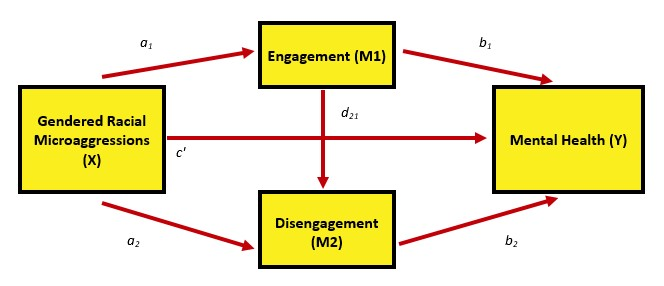
\includegraphics{images/CompMed/LewisSerialMed.jpg}
\caption{An image of the serial mediation we will work}
\end{figure}

Our parallel multiple mediator model of gendered racial microaggressions on mental health through engagement and disengagement coping strategies assumed no causal association between the mediators. Noting the statistically significant correlation between engagement and disengagement, what if engagement influenced disengagement, which, in turn influenced mental health.

If this is our goal (image), how many direct and indirect effects are contained in this model? Using the same processes as before, let's plan our model:

\begin{itemize}
\tightlist
\item
  We add a path predicting disengagement from engagement, and label it with a \(d_{21}\)

  \begin{itemize}
  \tightlist
  \item
    Regarding the notation, it makes sense that we use a \emph{d} to designate a new type of path; I don't know why we use a subscript of 21
  \end{itemize}
\item
  We specify a third indirect path that multiplies those 3 paths (a1, d21, b2) together
\item
  We add a third contrast so that we get all the combinations of indirect comparisons: 1-2, 1-3 2-3
\item
  We update our total\_indirects calculation to include indirect\#3
\item
  We update our total\_c calculation to include indirect\#3
\end{itemize}

\hypertarget{specify-the-lavaan-model}{%
\subsection{\texorpdfstring{Specify the \emph{lavaan} model}{Specify the lavaan model}}\label{specify-the-lavaan-model}}

\begin{Shaded}
\begin{Highlighting}[]
\FunctionTok{set.seed}\NormalTok{(}\DecValTok{210403}\NormalTok{)}
\FunctionTok{library}\NormalTok{(lavaan)}
\NormalTok{serial\_Lewis }\OtherTok{\textless{}{-}} \StringTok{\textquotesingle{}}
\StringTok{    MtnlHlth \textasciitilde{} b1*Engmt + b2*DisEngmt + c\_p*GRMS}
\StringTok{    Engmt \textasciitilde{} a1*GRMS    }
\StringTok{    DisEngmt \textasciitilde{} a2*GRMS}
\StringTok{    DisEngmt \textasciitilde{} d21*Engmt}
\StringTok{    indirect1 := a1 * b1}
\StringTok{    indirect2 := a2 * b2}
\StringTok{    indirect3 := a1 * d21 * b2}
\StringTok{    contrast1 := indirect1 {-} indirect2}
\StringTok{    contrast2 := indirect1 {-} indirect3}
\StringTok{    contrast3 := indirect2 {-} indirect3}
\StringTok{    total\_indirects := indirect1 + indirect2 + indirect3}
\StringTok{    total\_c := c\_p + indirect1 + indirect2 + indirect3}
\StringTok{    direct := c\_p}
\StringTok{\textquotesingle{}}
\NormalTok{serial\_Lewis\_fit }\OtherTok{\textless{}{-}} \FunctionTok{sem}\NormalTok{(serial\_Lewis, }\AttributeTok{data =}\NormalTok{ Lewis\_df, }\AttributeTok{se =} \StringTok{"bootstrap"}\NormalTok{, }\AttributeTok{missing =} \StringTok{\textquotesingle{}fiml\textquotesingle{}}\NormalTok{, }\AttributeTok{bootstrap =} \DecValTok{1000}\NormalTok{)}
\NormalTok{sLewis\_sum }\OtherTok{\textless{}{-}} \FunctionTok{summary}\NormalTok{(serial\_Lewis\_fit, }\AttributeTok{standardized =} \ConstantTok{TRUE}\NormalTok{, }\AttributeTok{rsq=}\NormalTok{T, }\AttributeTok{fit=}\ConstantTok{TRUE}\NormalTok{, }\AttributeTok{ci=}\ConstantTok{TRUE}\NormalTok{)    }
\NormalTok{sLewis\_ParEsts }\OtherTok{\textless{}{-}} \FunctionTok{parameterEstimates}\NormalTok{(serial\_Lewis\_fit, }\AttributeTok{boot.ci.type =} \StringTok{"bca.simple"}\NormalTok{, }\AttributeTok{standardized=}\ConstantTok{TRUE}\NormalTok{)}
\end{Highlighting}
\end{Shaded}

\begin{Shaded}
\begin{Highlighting}[]
\NormalTok{sLewis\_sum}
\end{Highlighting}
\end{Shaded}

\begin{verbatim}
## lavaan 0.6.16 ended normally after 1 iteration
## 
##   Estimator                                         ML
##   Optimization method                           NLMINB
##   Number of model parameters                        12
## 
##   Number of observations                           212
##   Number of missing patterns                         1
## 
## Model Test User Model:
##                                                       
##   Test statistic                                 0.000
##   Degrees of freedom                                 0
## 
## Model Test Baseline Model:
## 
##   Test statistic                               155.625
##   Degrees of freedom                                 6
##   P-value                                        0.000
## 
## User Model versus Baseline Model:
## 
##   Comparative Fit Index (CFI)                    1.000
##   Tucker-Lewis Index (TLI)                       1.000
##                                                       
##   Robust Comparative Fit Index (CFI)             1.000
##   Robust Tucker-Lewis Index (TLI)                1.000
## 
## Loglikelihood and Information Criteria:
## 
##   Loglikelihood user model (H0)               -868.431
##   Loglikelihood unrestricted model (H1)       -868.431
##                                                       
##   Akaike (AIC)                                1760.862
##   Bayesian (BIC)                              1801.141
##   Sample-size adjusted Bayesian (SABIC)       1763.117
## 
## Root Mean Square Error of Approximation:
## 
##   RMSEA                                          0.000
##   90 Percent confidence interval - lower         0.000
##   90 Percent confidence interval - upper         0.000
##   P-value H_0: RMSEA <= 0.050                       NA
##   P-value H_0: RMSEA >= 0.080                       NA
##                                                       
##   Robust RMSEA                                   0.000
##   90 Percent confidence interval - lower         0.000
##   90 Percent confidence interval - upper         0.000
##   P-value H_0: Robust RMSEA <= 0.050                NA
##   P-value H_0: Robust RMSEA >= 0.080                NA
## 
## Standardized Root Mean Square Residual:
## 
##   SRMR                                           0.000
## 
## Parameter Estimates:
## 
##   Standard errors                            Bootstrap
##   Number of requested bootstrap draws             1000
##   Number of successful bootstrap draws            1000
## 
## Regressions:
##                    Estimate  Std.Err  z-value  P(>|z|) ci.lower ci.upper
##   MtnlHlth ~                                                            
##     Engmt     (b1)    0.581    0.431    1.346    0.178   -0.287    1.447
##     DisEngmt  (b2)   -3.750    0.471   -7.954    0.000   -4.670   -2.851
##     GRMS     (c_p)   -0.575    0.243   -2.363    0.018   -1.071   -0.126
##   Engmt ~                                                               
##     GRMS      (a1)    0.203    0.044    4.584    0.000    0.116    0.292
##   DisEngmt ~                                                            
##     GRMS      (a2)    0.193    0.038    5.150    0.000    0.117    0.266
##     Engmt    (d21)    0.236    0.057    4.163    0.000    0.132    0.355
##    Std.lv  Std.all
##                   
##     0.581    0.092
##    -3.750   -0.519
##    -0.575   -0.135
##                   
##     0.203    0.300
##                   
##     0.193    0.329
##     0.236    0.271
## 
## Intercepts:
##                    Estimate  Std.Err  z-value  P(>|z|) ci.lower ci.upper
##    .MtnlHlth         27.728    1.027   27.004    0.000   25.525   29.753
##    .Engmt             1.915    0.100   19.140    0.000    1.720    2.110
##    .DisEngmt          0.818    0.128    6.400    0.000    0.564    1.073
##    Std.lv  Std.all
##    27.728    7.257
##     1.915    3.147
##     0.818    1.547
## 
## Variances:
##                    Estimate  Std.Err  z-value  P(>|z|) ci.lower ci.upper
##    .MtnlHlth         10.067    0.846   11.895    0.000    8.249   11.477
##    .Engmt             0.337    0.035    9.718    0.000    0.270    0.402
##    .DisEngmt          0.214    0.019   11.318    0.000    0.175    0.249
##    Std.lv  Std.all
##    10.067    0.690
##     0.337    0.910
##     0.214    0.765
## 
## R-Square:
##                    Estimate
##     MtnlHlth          0.310
##     Engmt             0.090
##     DisEngmt          0.235
## 
## Defined Parameters:
##                    Estimate  Std.Err  z-value  P(>|z|) ci.lower ci.upper
##     indirect1         0.118    0.095    1.249    0.212   -0.062    0.310
##     indirect2        -0.726    0.169   -4.295    0.000   -1.067   -0.417
##     indirect3        -0.180    0.065   -2.750    0.006   -0.337   -0.076
##     contrast1         0.844    0.207    4.069    0.000    0.471    1.252
##     contrast2         0.298    0.125    2.384    0.017    0.089    0.572
##     contrast3        -0.546    0.180   -3.028    0.002   -0.896   -0.206
##     total_indircts   -0.787    0.185   -4.259    0.000   -1.152   -0.440
##     total_c          -1.362    0.253   -5.392    0.000   -1.841   -0.864
##     direct           -0.575    0.243   -2.362    0.018   -1.071   -0.126
##    Std.lv  Std.all
##     0.118    0.028
##    -0.726   -0.170
##    -0.180   -0.042
##     0.844    0.198
##     0.298    0.070
##    -0.546   -0.128
##    -0.787   -0.185
##    -1.362   -0.320
##    -0.575   -0.135
\end{verbatim}

\begin{Shaded}
\begin{Highlighting}[]
\NormalTok{sLewis\_ParEsts}
\end{Highlighting}
\end{Shaded}

\begin{verbatim}
##                lhs op                               rhs           label    est
## 1         MtnlHlth  ~                             Engmt              b1  0.581
## 2         MtnlHlth  ~                          DisEngmt              b2 -3.750
## 3         MtnlHlth  ~                              GRMS             c_p -0.575
## 4            Engmt  ~                              GRMS              a1  0.203
## 5         DisEngmt  ~                              GRMS              a2  0.193
## 6         DisEngmt  ~                             Engmt             d21  0.236
## 7         MtnlHlth ~~                          MtnlHlth                 10.067
## 8            Engmt ~~                             Engmt                  0.337
## 9         DisEngmt ~~                          DisEngmt                  0.214
## 10            GRMS ~~                              GRMS                  0.806
## 11        MtnlHlth ~1                                                   27.728
## 12           Engmt ~1                                                    1.915
## 13        DisEngmt ~1                                                    0.818
## 14            GRMS ~1                                                    1.990
## 15       indirect1 :=                             a1*b1       indirect1  0.118
## 16       indirect2 :=                             a2*b2       indirect2 -0.726
## 17       indirect3 :=                         a1*d21*b2       indirect3 -0.180
## 18       contrast1 :=               indirect1-indirect2       contrast1  0.844
## 19       contrast2 :=               indirect1-indirect3       contrast2  0.298
## 20       contrast3 :=               indirect2-indirect3       contrast3 -0.546
## 21 total_indirects :=     indirect1+indirect2+indirect3 total_indirects -0.787
## 22         total_c := c_p+indirect1+indirect2+indirect3         total_c -1.362
## 23          direct :=                               c_p          direct -0.575
##       se      z pvalue ci.lower ci.upper std.lv std.all std.nox
## 1  0.431  1.346  0.178   -0.339    1.354  0.581   0.092   0.092
## 2  0.471 -7.954  0.000   -4.703   -2.892 -3.750  -0.519  -0.519
## 3  0.243 -2.363  0.018   -1.047   -0.099 -0.575  -0.135  -0.150
## 4  0.044  4.584  0.000    0.116    0.292  0.203   0.300   0.334
## 5  0.038  5.150  0.000    0.117    0.267  0.193   0.329   0.366
## 6  0.057  4.163  0.000    0.141    0.366  0.236   0.271   0.271
## 7  0.846 11.895  0.000    8.599   11.773 10.067   0.690   0.690
## 8  0.035  9.718  0.000    0.279    0.414  0.337   0.910   0.910
## 9  0.019 11.318  0.000    0.183    0.257  0.214   0.765   0.765
## 10 0.000     NA     NA    0.806    0.806  0.806   1.000   0.806
## 11 1.027 27.004  0.000   25.599   29.794 27.728   7.257   7.257
## 12 0.100 19.140  0.000    1.719    2.109  1.915   3.147   3.147
## 13 0.128  6.400  0.000    0.542    1.047  0.818   1.547   1.547
## 14 0.000     NA     NA    1.990    1.990  1.990   2.216   1.990
## 15 0.095  1.249  0.212   -0.061    0.311  0.118   0.028   0.031
## 16 0.169 -4.295  0.000   -1.130   -0.452 -0.726  -0.170  -0.190
## 17 0.065 -2.750  0.006   -0.359   -0.084 -0.180  -0.042  -0.047
## 18 0.207  4.069  0.000    0.493    1.325  0.844   0.198   0.221
## 19 0.125  2.384  0.017    0.108    0.605  0.298   0.070   0.078
## 20 0.180 -3.028  0.002   -0.965   -0.227 -0.546  -0.128  -0.143
## 21 0.185 -4.259  0.000   -1.198   -0.471 -0.787  -0.185  -0.206
## 22 0.253 -5.392  0.000   -1.873   -0.891 -1.362  -0.320  -0.356
## 23 0.243 -2.362  0.018   -1.047   -0.099 -0.575  -0.135  -0.150
\end{verbatim}

\hypertarget{figures-and-tables-2}{%
\subsection{Figures and Tables}\label{figures-and-tables-2}}

\textbf{Table 2 }

\begin{longtable}[]{@{}
  >{\raggedright\arraybackslash}p{(\columnwidth - 0\tabcolsep) * \real{1.0000}}@{}}
\toprule\noalign{}
\begin{minipage}[b]{\linewidth}\raggedright
Model Coefficients Assessing Engagement and Disengagement Coping as Serial Mediators Between Predicting Mental Health from Gendered Racial Microaggressions
\end{minipage} \\
\midrule\noalign{}
\endhead
\bottomrule\noalign{}
\endlastfoot
\end{longtable}

\begin{longtable}[]{@{}
  >{\centering\arraybackslash}p{(\columnwidth - 22\tabcolsep) * \real{0.0492}}
  >{\centering\arraybackslash}p{(\columnwidth - 22\tabcolsep) * \real{0.0246}}
  >{\centering\arraybackslash}p{(\columnwidth - 22\tabcolsep) * \real{0.0656}}
  >{\centering\arraybackslash}p{(\columnwidth - 22\tabcolsep) * \real{0.0246}}
  >{\centering\arraybackslash}p{(\columnwidth - 22\tabcolsep) * \real{0.0656}}
  >{\centering\arraybackslash}p{(\columnwidth - 22\tabcolsep) * \real{0.0246}}
  >{\centering\arraybackslash}p{(\columnwidth - 22\tabcolsep) * \real{0.0820}}
  >{\centering\arraybackslash}p{(\columnwidth - 22\tabcolsep) * \real{0.3033}}
  >{\centering\arraybackslash}p{(\columnwidth - 22\tabcolsep) * \real{0.0246}}
  >{\raggedleft\arraybackslash}p{(\columnwidth - 22\tabcolsep) * \real{0.0984}}
  >{\centering\arraybackslash}p{(\columnwidth - 22\tabcolsep) * \real{0.1230}}
  >{\centering\arraybackslash}p{(\columnwidth - 22\tabcolsep) * \real{0.1148}}@{}}
\toprule\noalign{}
\endhead
\bottomrule\noalign{}
\endlastfoot
IV & & M1 & & M2 & & DV & \(B\) for \emph{a}, \emph{b}, and \(d_{21}\) paths & & \(B\) & \(SE\) & \(p\) \\
GRMS & --\textgreater{} & Engmt & --\textgreater{} & & & MntlHlth & (0.203) X (0.581) & = & 0.118 & 0.095 & 0.212 \\
GRMS & --\textgreater{} & DisEngmt & --\textgreater{} & & & MntlHlth & (0.193) X (-3.750) & = & -0.726 & 0.169 & 0.000 \\
GRMS & --\textgreater{} & Engmt & --\textgreater{} & DisEngmt & --\textgreater{} & MntlHlth & (0.203) X (0.236) X (-3.750) & = & -0.180 & 0.065 & 0.000 \\
\end{longtable}

\begin{longtable}[]{@{}
  >{\centering\arraybackslash}p{(\columnwidth - 6\tabcolsep) * \real{0.6846}}
  >{\centering\arraybackslash}p{(\columnwidth - 6\tabcolsep) * \real{0.0923}}
  >{\centering\arraybackslash}p{(\columnwidth - 6\tabcolsep) * \real{0.1154}}
  >{\centering\arraybackslash}p{(\columnwidth - 6\tabcolsep) * \real{0.1077}}@{}}
\toprule\noalign{}
\endhead
\bottomrule\noalign{}
\endlastfoot
& \(B\) & \(SE\) & \(p\) \\
Total indirect effect & -0.787 & 0.185 & 0.000 \\
Total effect of GRMS (X) on mental health (Y; c path) & -1.362 & 0.253 & 0.000 \\
Direct effect of GRMS (X) on mental health (Y; c' path) & -0.575 & 0.243 & 0.018 \\
Contrast comparing indirects 1 (via engagement) and 2 (via disengagement) & 0.844 & 0.207 & 0.000 \\
Contrast comparing indirects 1 (via engagement) and 3 (serially via disengagement) & 0.298 & 0.125 & 0.017 \\
Contrast comparing indirects 2 (via disengagement) and 3 (serially via disengagement) & -0.546 & 0.180 & 0.002 \\
\end{longtable}

\begin{longtable}[]{@{}
  >{\raggedright\arraybackslash}p{(\columnwidth - 0\tabcolsep) * \real{1.0000}}@{}}
\toprule\noalign{}
\endhead
\bottomrule\noalign{}
\endlastfoot
\end{longtable}

\emph{Note}. IV = gendered racial microaggressions; M1 = engagement coping; M2 = disengagement coping; Y = mental health. The significance of the indirect effects was calculated with bias-corrected confidence intervals (.95) bootstrap analysis.

Working through the data, we should be able to find these items:

\begin{itemize}
\tightlist
\item
  The model accounts for of the variance in predicting mental health outcomes.
\item
  The total effect of GRMS (X) on mental health (Y) is -1.362 (\(p\) = 0.000) is negative and statistically significant.
\item
  The direct effect of GRMS (X) on mental health (Y) (-0.575, \(p\) = 0.018) is still negative, but weaker in magnitude (relative to the total effect). While the \(p\) value is statistically significant, it is closer to being not significant (than the total effect). This reduction in magnitude and strength of significance is consistent with the Baron and Kenny \citeyearpar{baron_moderator-mediator_1986} logic of mediation.
\item
  Indirect effect \#1 (\(a_{1}\) x \(b_{1}\) or GRMS through engagement coping to mental health) is 0.118 (\(p\) = 0.212). Again, \(p\) is \textgreater{} .05. Examining the individual paths, there is a statistically significant relationship from GRMS to engagement, but not from engagement to mental health.
\item
  Indirect effect \#2 (\(a_{2}\) x \(b_{2}\), or GRMS through disengagement coping to mental health, is -0.726 (\(p\) = 0.000). Each of the paths is statistically significant from zero and so is the indirect effect.
\item
  Indirect effect \#3 (\(a_{2}\) x \(d_{21}\) x \(b_{2}\); GRMS through engagement coping through disengagement coping to mental health) is -0.180 (\(p\) = 0.000). This indirect effect involves \(a_{1}\) (GRMS to engagement) which is not significant. However, the remaining paths were significant. That is engagement coping led to increased disengagement coping, which led to poorer mental health outcomes.
\item
  Total indirect: -0.787 (\(p\) = 0.000) is the sum of all specific indirect effects and is statistically significant.
\item
  With \textbf{contrasts} we ask: Are the indirect effects statistically significantly different from each other?

  \begin{itemize}
  \tightlist
  \item
    Contrast 1 (indirect 1 v 2) = 0.844 (\(p\) = 0.000), yes
  \item
    Contrast 2 (indirect 1 v 3) = 0.844 (\(p\) = 0.017), yes
  \item
    Contrast 3 (indirect 2 v 3) = 0.844 (\(p\) = -0.546), yes
  \item
    This formal test of contrasts is an important one. It is not ok to infer that effects are statistically significantly different than each other on the basis of their estimates or \(p\) values. The formal test allows us to claim (with justification) that the strongest indirect effect is \#2 -- GRMS through disengagement coping to mental health.
  \end{itemize}
\end{itemize}

\begin{Shaded}
\begin{Highlighting}[]
\FunctionTok{library}\NormalTok{(semTable)}
\NormalTok{LewisserialTbl }\OtherTok{\textless{}{-}} \FunctionTok{semTable}\NormalTok{(serial\_Lewis\_fit, }\AttributeTok{columns =} \FunctionTok{c}\NormalTok{(}\StringTok{"est"}\NormalTok{, }\StringTok{"se"}\NormalTok{, }\StringTok{"p"}\NormalTok{, }\StringTok{"rsquare"}\NormalTok{),  }\AttributeTok{columnLabels =} \FunctionTok{c}\NormalTok{(}\AttributeTok{eststars =} \StringTok{"Estimate"}\NormalTok{), }\AttributeTok{paramSets =} \FunctionTok{c}\NormalTok{(}\StringTok{"composites"}\NormalTok{, }\StringTok{"loadings"}\NormalTok{, }\StringTok{"slopes"}\NormalTok{, }\StringTok{"intercepts"}\NormalTok{, }\StringTok{"residualvariances"}\NormalTok{), }\AttributeTok{file =} \StringTok{"LewisSerialTbl"}\NormalTok{, }\AttributeTok{type =} \StringTok{"csv"}\NormalTok{, }\AttributeTok{print.results =} \ConstantTok{TRUE}\NormalTok{)}
\end{Highlighting}
\end{Shaded}

This is not the greatest figure. There is much to learn in \emph{semPlot}.

\begin{Shaded}
\begin{Highlighting}[]
\FunctionTok{semPaths}\NormalTok{(serial\_Lewis\_fit, }\CommentTok{\#must identiy the model you want to map}
         \AttributeTok{what =} \StringTok{"est"}\NormalTok{, }\CommentTok{\#"est" plots the estimates, but keeps it greyscale with no fading}
         \CommentTok{\#whatLabels = "stand", \#"stand" changes to standardized values}
         \CommentTok{\#layout = \textquotesingle{}tree\textquotesingle{}, rotation = 2, \#together, puts predictors on left, IVs on right }
         \AttributeTok{layout =} \StringTok{\textquotesingle{}circle\textquotesingle{}}\NormalTok{,}
         \AttributeTok{edge.label.cex =} \FloatTok{1.00}\NormalTok{, }\CommentTok{\#font size of parameter values}
         \CommentTok{\#edge.color = "black", \#overwrites the green/black coloring}
         \AttributeTok{sizeMan=}\DecValTok{10}\NormalTok{, }\CommentTok{\#size of squares/observed/"manifest" variables}
         \AttributeTok{fade=}\ConstantTok{FALSE}\NormalTok{, }\CommentTok{\#if TRUE, there lines are faded such that weaker lines correspond with lower values {-}{-} a cool effect, but tough for journals}
         \AttributeTok{esize=}\DecValTok{2}\NormalTok{, }
         \AttributeTok{asize=}\DecValTok{3}\NormalTok{,}
         \CommentTok{\#label.prop = .5,}
         \AttributeTok{label.font =} \FloatTok{2.5}\NormalTok{, }\CommentTok{\#controls size (I think) of font for labels}
         \AttributeTok{label.scale =} \ConstantTok{TRUE}\NormalTok{, }\CommentTok{\#if false, the labels will not scale to fit inside the nodes}
         \AttributeTok{nDigits =} \DecValTok{3}\NormalTok{, }\CommentTok{\#decimal places (default is 2)}
         \AttributeTok{residuals =} \ConstantTok{FALSE}\NormalTok{,}\CommentTok{\#excludes residuals (and variances) from the path diagram}
         \AttributeTok{nCharNodes =} \DecValTok{0}\NormalTok{, }\CommentTok{\#specifies how many characters to abbreviate variable lables; default is 3.  If 0, uses your entire variable label and adjusts fontsize (which could be a downside)}
         \AttributeTok{intercepts =} \ConstantTok{FALSE}\NormalTok{, }\CommentTok{\#gets rid of those annoying triangles (intercepts) in the path diagram)}
\NormalTok{)}
\FunctionTok{title}\NormalTok{(}\StringTok{"The Effect of Gendered Racial Microaggressions on Mental Health through Engaged and Disengaged Coping Styles"}\NormalTok{)}
\end{Highlighting}
\end{Shaded}

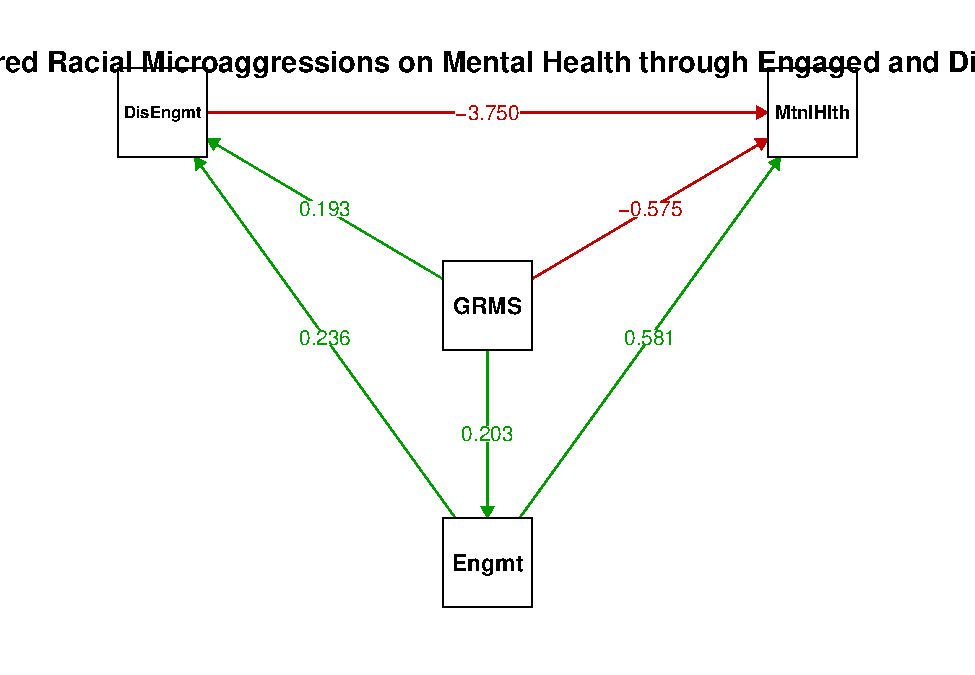
\includegraphics{06-ComplexMed_files/figure-latex/semPlot of serial PMI model-1.pdf}

\hypertarget{apa-style-writeup-2}{%
\subsection{APA Style Writeup}\label{apa-style-writeup-2}}

\textbf{Method} \textbf{Data Analysis} Serial multiple mediation is appropriate when testing the influence of an independent variable (X) on the dependent variable (Y) directly, as well as indirectly through two or more mediators (M) and there is reason to hypothesize that variables that are causally prior in the model affect all variables later in the causal sequence \citep{hayes_introduction_2018}. We utilized serial multiple mediation analysis to test the influence of gendered racial microaggressions (X, GRMS) on mental health (Y, MntlHlth) directly as well as indirectly through the mediators engagement coping (M1, Engmt) and disengagement coping (M2, DisEngmt). Moreover, we hypothesized a causal linkage between from the engagement coping mediator to the disengagement coping mediator such that a third specific indirect effect began with GRMS (X) through engagement coping (M1) through disengagement coping (M2) to mental health (Y). Using the \emph{lavaan} (v. 0.6-7) package in R we followed the procedures outlined in Hayes \citeyearpar{hayes_introduction_2018} by analyzing the strength and significance of four sets of effects: specific indirect, the total indirect, the direct, and total. Bootstrap analysis, a nonparametric sampling procedure, was used to test the significance of the indirect effects.

\emph{Hayes would likely recommend that we say this with fewer acronyms and more words/story.}

\textbf{Results} \textbf{Preliminary Analyses} Descriptive statistics were computed, and all variables were assessed univariate normality. \emph{You would give your results regarding skew, kurtosis, Shapiro Wilks', here. If relevant, you could also describe multivariate normality.} A summary of descriptive statistics and a correlation matrix for the study is provided in Table 1. These bivariate relations provide evidence to support the test of mediation analysis.

\textbf{Serial Multiple Mediation Analysis} A model of serial multiple mediation was analyzed examining the degree to which engagement and disengagement coping mediated the relationship between gendered racial microaggressions and mental health outcomes. Hayes \citeyearpar{hayes_introduction_2018} recommended this strategy over simple mediation models because it allows for all mediators to be examined, simultaneously and allows the testing of the seriated effect of prior mediators onto subsequent ones. Using the \emph{lavaan} (v. 0.6-7) package in R, coefficients for specific indirect, total indirect, direct, and total were computed. Path coefficients refer to regression weights, or slopes, of the expected changes in the dependent variable given a unit change in the independent variables.

Results (depicted in Figure \# and presented in Table \#) suggest that of the variance in behavioral intentions is accounted for by the three variables in the model. Two of the specific indirect effects were significant and were statistically significantly different from each other. Specifically, the effect of gendered racial microaggressions through disengagement coping to mental health (\(B\) = 0.118, \(p\) = 0.212) was stronger than the indirect effect from gendered racial microaggressions through engagement coping through disengagement coping to mental health (\(B\) = -0.180, \(p\) = 0.000). Interpreting the results suggests that, mental health outcomes are negatively impacted by gendered racial microaggressions direct and indirectly through disengagement coping. It is this latter path that has the greatest impact.

\emph{Note}: In a manner consistent with the Lewis et al. \citeyearpar{lewis_applying_2017} article, the APA Results section can be fairly short. This is especially true when a well-organized table presents the results. In fact, I oculd have left all the numbers out of this except for the \(R^2\) (because it was not reported in the table).

\hypertarget{troubleshooting-and-faqs}{%
\section{Troubleshooting and FAQs}\label{troubleshooting-and-faqs}}

An indirect effect that was (seemingly) significant in a simple (single) mediation disappears when additional mediators are added.

\begin{itemize}
\tightlist
\item
  Correlated mediators (e.g., multicollinearity) is a likely possibility.
\item
  Which is correct? Maybe both\ldots{}
\end{itemize}

A total effect was not significant, but there is one or more statistically significant specific indirect effect

\begin{itemize}
\tightlist
\item
  Recall that a total effect equals the sum of direct and indirect effects. If one specific indirect effect is positive and another is negative, this could account for the NS total effect.
\item
  If the direct effect is NS, but the indirect effects are significant, this might render the total effect NS.
\item
  The indirect effects might operate differently in subpopulations (males, females).
\end{itemize}

Your editor/peer reviewer/dissertation chair-or-committee member may insist that you do this the Baron \& Kenny way (aka ``the causal steps approach'').

\begin{itemize}
\tightlist
\item
  Hayes 4.1 \citeyearpar{hayes_introduction_2018} provides fabulous narration and justification for how to justify your (I believe correct) decision to just use the PROCESS (aka, bootstrapped, bias corrected, CIs )approach.
\item
  My favorite line in his text reads, '' (the B\&K way).is still being taught and recommended by researchers who don't follow the methodology literature.''
\end{itemize}

How can I extend a mediation (only) model to include multiple Xs, Ys, or COVs?

\begin{itemize}
\tightlist
\item
  There is fabulous, fabulous narration and syntax for doing all of this in Hayes text. Of course his mechanics are in PROCESS, but \emph{lavaan} is easy to use by just ``drawing more paths'' via the syntax. We'll get more practice as we go along.
\end{itemize}

What about effect sizes? Shouldn't we be including/reporting them?

\begin{itemize}
\tightlist
\item
  Yes! The closest thing we have reported to an effect size is \(R^2\), which assess proportion of variance accounted for in the M and Y variables.\\
\item
  In PROCESS and path analysis this is still emerging. Hayes chapter 4 presents a handful of options for effect sizes beyond \(R^2\).
\end{itemize}

\hypertarget{practice-problems-5}{%
\section{Practice Problems}\label{practice-problems-5}}

The three problems described below are designed to be grow in this series of chapters that begins with simple mediation and progresses through complex mediation, moderated moderation, and conditional process analysis. I recommend that you select a dataset that includes at least four variables. If you are new to this topic, you may wish to select variables that are all continuously scaled. The IV and moderator (in subsequent chapters) could be categorical (if they are dichotomous, please use 0/1 coding; if they have more than one category it is best if they are ordered). You will likely encounter challenges that were not covered in this chapter. Search for and try out solutions, knowing that there are multiple paths through the analysis.

The suggested practice problem for this chapter is to conduct a parallel or serial mediation (or both).

\hypertarget{problem-1-rework-the-research-vignette-as-demonstrated-but-change-the-random-seed-1}{%
\subsection{Problem \#1: Rework the research vignette as demonstrated, but change the random seed}\label{problem-1-rework-the-research-vignette-as-demonstrated-but-change-the-random-seed-1}}

If this topic feels a bit overwhelming, simply change the random seed in the data simulation, then rework the problem. This should provide minor changes to the data (maybe in the second or third decimal point), but the results will likely be very similar.

\begin{longtable}[]{@{}
  >{\raggedright\arraybackslash}p{(\columnwidth - 4\tabcolsep) * \real{0.7642}}
  >{\centering\arraybackslash}p{(\columnwidth - 4\tabcolsep) * \real{0.1220}}
  >{\centering\arraybackslash}p{(\columnwidth - 4\tabcolsep) * \real{0.1138}}@{}}
\toprule\noalign{}
\begin{minipage}[b]{\linewidth}\raggedright
Assignment Component
\end{minipage} & \begin{minipage}[b]{\linewidth}\centering
\end{minipage} & \begin{minipage}[b]{\linewidth}\centering
\end{minipage} \\
\midrule\noalign{}
\endhead
\bottomrule\noalign{}
\endlastfoot
1. Assign each variable to the X, Y, M1, and M2 roles (ok but not required to include a cov) & 5 & \_\_\_\_\_ \\
2. Specify and run the lavaan model & 5 & \_\_\_\_\_ \\
3. Use semPlot to create a figure & 5 & \_\_\_\_\_ \\
4. Create a table that includes a summary of the effects (indirect, direct, total, total indirect) as well as contrasts (if you chose a serially mediated model) & 5 & \_\_\_\_\_ \\
5. Represent your work in an APA-style write-up & 5 & \_\_\_\_\_ \\
6. Explanation to grader & 5 & \_\_\_\_\_ \\
7. Be able to hand-calculate the indirect, direct, and total effects from the a, b, \& c' paths & 5 & \_\_\_\_\_ \\
\textbf{Totals} & 35 & \_\_\_\_\_ \\
\end{longtable}

\hypertarget{problem-2-rework-the-research-vignette-but-swap-one-or-more-variables-1}{%
\subsection{Problem \#2: Rework the research vignette, but swap one or more variables}\label{problem-2-rework-the-research-vignette-but-swap-one-or-more-variables-1}}

Use the simulated data provided in this chapter, but swap out one or more of the variables. This could mean changing roles for the variables that were the focus of the chapter, or substituting one or more variables for those in the simulated data but not modeled in the chapter.

\begin{longtable}[]{@{}
  >{\raggedright\arraybackslash}p{(\columnwidth - 4\tabcolsep) * \real{0.7642}}
  >{\centering\arraybackslash}p{(\columnwidth - 4\tabcolsep) * \real{0.1220}}
  >{\centering\arraybackslash}p{(\columnwidth - 4\tabcolsep) * \real{0.1138}}@{}}
\toprule\noalign{}
\begin{minipage}[b]{\linewidth}\raggedright
Assignment Component
\end{minipage} & \begin{minipage}[b]{\linewidth}\centering
\end{minipage} & \begin{minipage}[b]{\linewidth}\centering
\end{minipage} \\
\midrule\noalign{}
\endhead
\bottomrule\noalign{}
\endlastfoot
1. Assign each variable to the X, Y, M1, and M2 roles (ok but not required to include a cov) & 5 & \_\_\_\_\_ \\
2. Specify and run the lavaan model & 5 & \_\_\_\_\_ \\
3. Use semPlot to create a figure & 5 & \_\_\_\_\_ \\
4. Create a table that includes a summary of the effects (indirect, direct, total, total indirect) as well as contrasts (if you chose a serially mediated model) & 5 & \_\_\_\_\_ \\
5. Represent your work in an APA-style write-up & 5 & \_\_\_\_\_ \\
6. Explanation to grader & 5 & \_\_\_\_\_ \\
7. Be able to hand-calculate the indirect, direct, and total effects from the a, b, \& c' paths & 5 & \_\_\_\_\_ \\
\textbf{Totals} & 35 & \_\_\_\_\_ \\
\end{longtable}

\hypertarget{problem-3-use-other-data-that-is-available-to-you-1}{%
\subsection{Problem \#3: Use other data that is available to you}\label{problem-3-use-other-data-that-is-available-to-you-1}}

Use data for which you have permission and access. This could be IRB approved data you have collected or from your lab; data you simulate from a published article; data from an open science repository; or data from other chapters in this OER.

\begin{longtable}[]{@{}
  >{\raggedright\arraybackslash}p{(\columnwidth - 4\tabcolsep) * \real{0.7642}}
  >{\centering\arraybackslash}p{(\columnwidth - 4\tabcolsep) * \real{0.1220}}
  >{\centering\arraybackslash}p{(\columnwidth - 4\tabcolsep) * \real{0.1138}}@{}}
\toprule\noalign{}
\begin{minipage}[b]{\linewidth}\raggedright
Assignment Component
\end{minipage} & \begin{minipage}[b]{\linewidth}\centering
\end{minipage} & \begin{minipage}[b]{\linewidth}\centering
\end{minipage} \\
\midrule\noalign{}
\endhead
\bottomrule\noalign{}
\endlastfoot
1. Assign each variable to the X, Y, M1, and M2 roles (ok but not required to include a cov) & 5 & \_\_\_\_\_ \\
2. Specify and run the lavaan model & 5 & \_\_\_\_\_ \\
3. Use semPlot to create a figure & 5 & \_\_\_\_\_ \\
4. Create a table that includes a summary of the effects (indirect, direct, total, total indirect) as well as contrasts (if you chose a serially mediated model) & 5 & \_\_\_\_\_ \\
5. Represent your work in an APA-style write-up & 5 & \_\_\_\_\_ \\
6. Explanation to grader & 5 & \_\_\_\_\_ \\
7. Be able to hand-calculate the indirect, direct, and total effects from the a, b, \& c' paths & 5 & \_\_\_\_\_ \\
\textbf{Totals} & 35 & \_\_\_\_\_ \\
\end{longtable}

  \bibliography{STATSnMETH.bib}

\end{document}
